\RequirePackage[l2tabu,orthodox]{nag}
\documentclass[a5paper,10pt,twoside,openany,article]{memoir}

%!TEX root = ../dissertation.tex
\usepackage{etoolbox}
\usepackage{pdflscape}
\usepackage{geometry}
\usepackage{xparse}

%% Various maths
\usepackage{amsthm,amsmath,amscd,amsfonts,amssymb,mathtools,amsthm,systeme}
\DeclareMathOperator\erf{erf}
%% Localization
\usepackage[main=russian,german,english]{babel}
\usepackage{fontspec}
\usepackage{iflang}

% for external links
\usepackage{xr}
% \makeatletter
% \newcommand*{\addFileDependency}[1]{% argument=file name and extension
%   \typeout{(#1)}
%   \@addtofilelist{#1}
%   \IfFileExists{#1}{}{\typeout{No file #1.}}
% }
% \makeatother
% \newcommand*{\myexternaldocument}[1]{%
%     \externaldocument{#1}%
%     \addFileDependency{#1.tex}%
%     \addFileDependency{#1.aux}%
% }


\providecommand{\noopsort}[1]{}
%% Fonts
\setmonofont{Courier New}
\defaultfontfeatures{Ligatures=TeX}
\setmainfont{Times New Roman}
\setsansfont{Arial}

%% Page geometry
\geometry{a5paper, top=14mm, bottom=14mm, inner=18mm, outer=10mm, footskip=5mm, nomarginpar}
\setlength{\topskip}{0pt}
\setlength{\footskip}{12.3pt}
\SingleSpacing

\makeevenhead{plain}{}{\thepage}{}
\makeoddhead{plain}{}{\thepage}{}
\makeevenfoot{plain}{}{}{}
\makeoddfoot{plain}{}{}{}
\pagestyle{plain}

%% Penalties
\tolerance=1414
\hbadness=1414
\emergencystretch=1.5em
\hfuzz=0.3pt
\vfuzz=\hfuzz
\clubpenalty=10000
\widowpenalty=10000
\brokenpenalty=4991

% \usepackage{totcount}
% \usepackage{lastpage}
% \regtotcounter[auxfile=totals.aux]{figure}
% \regtotcounter[auxfile=totals.aux]{table}
% \regtotcounter[auxfile=totals.aux]{page}
% \regtotcounter[auxfile=totals.aux]{algorithm}
% \newtotcounter[auxfile=totals.aux]{citnum}
% \newtotcounter[auxfile=totals.aux]{appendix}

%% Tuning of Table of Contents
\renewcommand{\cftchapterdotsep}{\cftdotsep}
\setrmarg{2.55em plus1fil}
\renewcommand{\cftchapterpagefont}{\normalfont}
\renewcommand{\cftchapterleader}{\cftdotfill{\cftchapterdotsep}}

% вот это чтобы были точки после номеров глав и подглав в содержании:
\renewcommand{\cftchapteraftersnum}{.\space}
\renewcommand{\cftsectionaftersnum}{.} 
\renewcommand{\cftsubsectionaftersnum}{.}

% чтобы были точки после номеров подразделов в тексте диссера
\AtBeginDocument{\setsecnumformat{\csname the#1\endcsname.~}}
\renewcommand*{\cftappendixname}{\appendixname\space}

%% Tuning of List of Figures/Tables
\makeatletter
\renewcommand{\@tocrmarg}{4em}
\renewcommand{\@pnumwidth}{3em}
\makeatother

%% Fonts and intervals of the basic things
%% Вот это задает отступы сверху и снизу от заголовкой и под-заголовков.
\newcommand{\basegostsectionfont}{\fontsize{10pt}{12pt}\selectfont\bfseries}
\newlength{\gostindent}
\setlength{\gostindent}{15pt}
% \setbeforesecskip{\gostindent}
% \setaftersecskip{\gostindent}
% \setbeforesubsecskip{\gostindent}
% \setaftersubsecskip{\gostindent}
% \setbeforesubsubsecskip{\gostindent}
% \setaftersubsubsecskip{\gostindent}

\makechapterstyle{thesisgost}{%
\chapterstyle{default}%
\setlength{\beforechapskip}{0pt}%
\setlength{\midchapskip}{0pt}%
\setlength{\afterchapskip}{\gostindent}%
\renewcommand*{\chapnamefont}{\basegostsectionfont}%
\renewcommand*{\chapnumfont}{\basegostsectionfont}%
\renewcommand*{\chaptitlefont}{\basegostsectionfont}%
\renewcommand*{\chapterheadstart}{}%
 \renewcommand*{\afterchapternum}{\quad}% <noscode> Ставит пробел между номером главы и названием в тексте, если закомментировать, то будет перенос строки
\renewcommand*{\printchapternum}{\centering\chapnumfont\thechapter}%
\renewcommand*{\printchaptername}{}%
\renewcommand*{\printchapternonum}{\centering}}

\makeatletter
\makechapterstyle{thesisgostchapname}{%
    \chapterstyle{thesisgost}
    \renewcommand*{\printchapternum}{\chapnumfont \thechapter .}   % точка после номера главы в тексте
    \renewcommand*{\printchaptername}{\centering\chapnamefont\@chapapp} %
}
\makeatother

\chapterstyle{thesisgost}
\setsecheadstyle{\basegostsectionfont\centering}
\setsecindent{0pt}
\setsubsecheadstyle{\basegostsectionfont\centering}
\setsubsecindent{0pt}
\setsubsubsecheadstyle{\basegostsectionfont\centering}
\setsubsubsecindent{0pt}
\sethangfrom{\noindent #1}

\chapterstyle{thesisgostchapname}
\renewcommand*{\cftchaptername}{\chaptername\space}

%% Making all the counters global
\counterwithout{equation}{chapter}
\counterwithout{equation}{section}
\counterwithout{equation}{subsection}
\counterwithout{figure}{chapter}
\counterwithout{figure}{section}
\counterwithout{figure}{subsection}
\counterwithout{table}{chapter}
\counterwithout{table}{section}
\counterwithout{table}{subsection}

\AtBeginDocument{%
\regtotcounter{totalcount@figure}%
\regtotcounter{totalcount@table}%
\regtotcounter{totalcount@algorithm}%
\regtotcounter{TotPages}%
}

%% Some not yet used magic to form Russian messages about sizes and counts
%% http://www.linux.org.ru/forum/general/6993203#comment-6994589 (используется totcount)
\makeatletter
\def\formbytotal#1#2#3#4#5{%
    \newcount\@c
    \@c\totvalue{#1}\relax
    \newcount\@last
    \newcount\@pnul
    \@last\@c\relax
    \divide\@last 10
    \@pnul\@last\relax
    \divide\@pnul 10
    \multiply\@pnul-10
    \advance\@pnul\@last
    \multiply\@last-10
    \advance\@last\@c
    \total{#1}~#2%
    \ifnum\@pnul=1#5\else%
    \ifcase\@last#5\or#3\or#4\or#4\or#4\else#5\fi
    \fi
}
\makeatother

%% A special environment for locale-dependent commands
%% Usage: \newlocalizedcommand{\YourCommandName}{expansion in English}{expansion in Russian}
%%        \renewlocalizedcommand{\YourCommandName}{expansion in English}{expansion in Russian}
\newcommand{\newlocalizedcommand}[3]{\newcommand{#1}{\IfLanguageName{russian}{#3}{#2}}}
\newcommand{\renewlocalizedcommand}[3]{\renewcommand{#1}{\IfLanguageName{russian}{#3}{#2}}}

%% Theorems (localized) %%
\newlocalizedcommand{\definitionname}{Definition}{Определение}
\newlocalizedcommand{\corollaryname}{Corollary}{Следствие}
\newlocalizedcommand{\theoremname}{Theorem}{Утверждение}
\newlocalizedcommand{\lemmaname}{Lemma}{Лемма}

\theoremstyle{definition}
\newtheorem{definition}{\definitionname}
\newtheorem{theorem}{\theoremname}
\newtheorem{lemma}{\lemmaname}
\newtheorem{corollary}{\corollaryname}

%% Paragraph formatting %%
\usepackage{indentfirst}
\AtBeginDocument{\setlength{\parindent}{2.5em}}

%% Enumerations (partially localized) %%
\usepackage{enumitem}
\setlist{nosep,labelindent=\parindent,leftmargin=*}

\makeatletter
\def\asbukx#1{\expandafter\@asbukx\csname c@#1\endcsname}
\def\@asbukx#1{\ifcase#1\or a\or б\or в\or г\or д\or е\or ж\or и\or к\or л\or м\or н\or п\or р\or с\or т\or у\or ф\or х\or ц\or ш\or щ\or э\or ю\or я\fi}
\def\Asbukx#1{\expandafter\@Asbukx\csname c@#1\endcsname}
\def\@Asbukx#1{\ifcase#1\or А\or Б\or В\or Г\or Д\or Е\or Ж\or И\or К\or Л\or М\or Н\or П\or Р\or С\or Т\or У\or Ф\or Х\or Ц\or Ш\or Щ\or Э\or Ю\or Я\fi}
\AddEnumerateCounter{\Asbukx}{\@Asbukx}{М}
\AddEnumerateCounter{\asbukx}{\@asbukx}{м}
\makeatother

\renewcommand{\labelitemi}{\normalfont\bfseries{--}}
\renewcommand\labelenumii{\arabic{enumii})}
\renewcommand\theenumii{\arabic{enumii}}
\renewlocalizedcommand{\labelenumi}{\alph{enumi})}{\asbukx{enumi})}
\renewlocalizedcommand{\theenumi}{\alph{enumi}}{\asbukx{enumi}}


%% Tuning of how floats look like
% We use floatrow/caption instead of memoir's poorly-working built-ins
\let\newfloat\undefined
\usepackage{caption}
\usepackage{floatrow}
\usepackage{subcaption}


%% Babel uses its own way to control captions, adhere to it
\addto{\captionsenglish}{%
\renewcommand{\figurename}{Figure}%
\renewcommand{\contentsname}{Contents}%
%\renewcommand{\ALG@name}{Algorithm}
}
\addto{\captionsrussian}{%
\renewcommand{\figurename}{Рисунок}%
\renewcommand{\contentsname}{Содержание}%
%\makeatletter
%\renewcommand{\ALG@name}{Листинг}%
%\makeatother
\renewcommand{\algorithmname}{Листинг}%
}

\floatsetup[figure]{style=plain, capposition=bottom}
\captionsetup[figure]{
    labelsep=endash,
    singlelinecheck=false,
    labelfont={normalsize,md},
    justification=centering,
    position=bottom
}
\floatsetup[table]{style=plain, capposition=top}
\captionsetup[table]{
    labelsep=endash,
    singlelinecheck=false,
    labelfont={normalsize,md},
    justification=justified,
    position=top
}
\floatsetup[algorithm]{style=plain, capposition=top}
\captionsetup[algorithm]{
    labelsep=endash,
    singlelinecheck=false,
    labelfont={normalsize,md},
    justification=justified,
    position=top
}

%\floatsetup[lstlisting]{style=plain, capposition=top}
%\captionsetup[lstlisting]{
%    labelsep=endash,
%    singlelinecheck=false,
%    labelfont={normalsize,md},
%    justification=justified,
%    position=top
%}

%% Tuning of table-of-contents

\settocdepth{subsection}            % до какого уровня подразделов выносить в оглавление
\setsecnumdepth{subsection}         % до какого уровня нумеровать подразделы

%% Custom math fonts

\usepackage{mathrsfs}

%% Graphics

\usepackage[dvipsnames, table, hyperref, cmyk]{xcolor}
\usepackage{graphicx}
\usepackage{pgfplots}
\pgfplotsset{compat=newest} 

% Include articles
\usepackage[final]{pdfpages}

%% Tables %%
\usepackage{tabularx}
\usepackage{longtable}
\usepackage{multirow,makecell}
\usepackage{hhline}
\usepackage{adjustbox}

\newcommand{\specialcell}[2][c]{%
  \begin{tabular}[#1]{@{}c@{}}#2\end{tabular}}

%% Hyperref %%
\usepackage{hyperref}
\definecolor{linkcolor}{rgb}{0,0,0}
\definecolor{citecolor}{rgb}{0,0,0}
\definecolor{urlcolor}{rgb}{0,0,0}

% No hypersetup here, as it needs some information not available here

%% Algorithmic environments %%
%\usepackage[linesnumbered,lined,boxed,commentsnumbered]{algorithm2e}
\usepackage{algorithm}
%\usepackage{algorithmic}
\usepackage[noend]{algpseudocode}
%\usepackage{amsmath}, amsthm,amsfonts,amssymb,amscd}

\algrenewcommand\algorithmicrequire{\textbf{Input:}}
\algrenewcommand\algorithmicensure{\textbf{Output:}}
\algnewcommand\algorithmicto{\textbf{to}}
\algrenewtext{For}[3] {\algorithmicfor\ $#1 \gets #2$ \algorithmicto\ $#3$ \algorithmicdo}
\algnewcommand\Continue{\textbf{continue}}
\algnewcommand\AndL{\textbf{and} }
\algnewcommand\OrL{\textbf{or} }
\algnewcommand\True{\textbf{True}}
\algnewcommand\False{\textbf{False}}

%% Counters
\usepackage[figure,table,algorithm]{totalcount}
\usepackage{totcount}
\usepackage{totpages}

%% Misc localization commands %%
\let\origle\le   \renewlocalizedcommand{\le}{\origle}{\leqslant}
\let\origleq\leq \renewlocalizedcommand{\leq}{\origleq}{\leqslant}
\let\origge\ge   \renewlocalizedcommand{\ge}{\origge}{\geqslant}
\let\origgeq\geq \renewlocalizedcommand{\geq}{\origgeq}{\geqslant}
\let\origtan\tan \renewlocalizedcommand{\tan}{\origtan}{\operatorname{tg}}
\let\origcot\cot \renewlocalizedcommand{\cot}{\origcot}{\operatorname{ctg}}
\let\origcsc\csc \renewlocalizedcommand{\csc}{\origcsc}{\operatorname{cosec}}
\let\origempty\emptyset \renewlocalizedcommand{\emptyset}{\origempty}{\varnothing}

%% Misc technical things %%
\newcommand{\resetfloatcounters}{%
\setcounter{figure}{0}%
\setcounter{table}{0}%
\setcounter{theorem}{0}%
\setcounter{lemma}{0}%
\setcounter{definition}{0}%
\setcounter{corollary}{0}%
\setcounter{footnote}{0}%
}

%% Bibliography packages and configuration

\usepackage{csquotes} % biblatex рекомендует его подключать. Пакет для оформления сложных блоков цитирования.

%%% Загрузка пакета с основными настройками %%%
\makeatletter
\usepackage[backend=biber,% движок
bibencoding=utf8,% кодировка bib файла
sorting=none,%nyt,% настройка сортировки списка литературы
style=gost-numeric,% стиль цитирования и библиографии (по ГОСТ)
language=autobib,% получение языка из babel/polyglossia, default: autobib % если ставить autocite или auto, то цитаты в тексте с указанием страницы, получат указание страницы на языке оригинала
autolang=other,% многоязычная библиография
clearlang=true,% внутренний сброс поля language, если он совпадает с языком из babel/polyglossia
defernumbers=true,% нумерация проставляется после двух компиляций, зато позволяет выцеплять библиографию по ключевым словам и нумеровать не из большего списка
sortcites=true,% сортировать номера затекстовых ссылок при цитировании (если в квадратных скобках несколько ссылок, то отображаться будут отсортированно, а не абы как)
movenames=false,% имена всегда в начале
maxbibnames=10,% показывать максимум 10 имен
]{biblatex}
\ltx@iffilelater{biblatex-gost.def}{2017/05/03}%
{%\toggletrue{bbx:gostbibliography}%
%\renewcommand*{\revsdnamepunct}{\addcomma}}{}
% <noscode> убрала addcomma чтобы не было запятых чежду last name и first name
\renewcommand*{\revsdnamepunct}{}}{}
\makeatother

% <noscode> замена точки с запятой на запятую при цитировании нескольких источников
\renewcommand*{\multicitedelim}{\addcomma\space}

\renewcommand*{\newblockpunct}{\addperiod\addnbspace---\space\bibsentence}

\DefineBibliographyStrings{english}{pages = {pp\adddot}}

\DefineBibliographyExtras{russian}{%
  \protected\def\bibrangedash{--\penalty\value{abbrvpenalty}}% almost unbreakable dash
  \protected\def\bibdaterangesep{\bibrangedash}%тире для дат
}
\DefineBibliographyExtras{english}{%
  \protected\def\bibrangedash{--\penalty\value{abbrvpenalty}}% almost unbreakable dash
  \protected\def\bibdaterangesep{\bibrangedash}%тире для дат
}

%Set higher penalty for breaking in number, dates and pages ranges
\setcounter{abbrvpenalty}{10000} % default is \hyphenpenalty which is 12
%Set higher penalty for breaking in names
\setcounter{highnamepenalty}{10000} % If you prefer the traditional BibTeX behavior (no linebreaks at highnamepenalty breakpoints), set it to ‘infinite’ (10 000 or higher).
\setcounter{lownamepenalty}{10000}

%% An environment which rewrites \cite to be \footfullcite for citations not in the author's list
\makeatletter
\newtoggle{footnotized@value}\togglefalse{footnotized@value}

\DeclareDocumentCommand{\trickycite}{oom}{%
\filteredcite{#3}%
\IfNoValueTF{#2}{%
\IfNoValueTF{#1}{%
% no #1 no #2
\iftoggle{footnotized@value}{\unspace\footfullcite{#3}}{\oldcite{#3}}%
}{%
% yes #1 no #2
\iftoggle{footnotized@value}{\unspace\footfullcite[#1]{#3}}{\oldcite[#1]{#3}}%
}}{
% yes #1 yes #2
\iftoggle{footnotized@value}{\unspace\footfullcite[#1][#2]{#3}}{\oldcite[#1][#2]{#3}}%
}}%
\newenvironment{footnotizeexcept}[1]{\begingroup%
\DeclareCiteCommand{\filteredcite}{}{\ifkeyword{#1}{\global\togglefalse{footnotized@value}}{\global\toggletrue{footnotized@value}}}{}{}%
\let\oldcite\cite\let\cite\trickycite}{\let\cite\oldcite\endgroup}
\makeatother

% make subfigure caption in russian
\renewcommand\thesubfigure{\asbuk{subfigure}}

%something for code listings
\usepackage{listings}

\usepackage{algorithm}
\usepackage{algpseudocode}

\algnewcommand\algorithmicforeach{\textbf{for}}
\algdef{S}[FOR]{For}[1]{\algorithmicforeach\ #1\ \algorithmicdo}

%\usepackage{fixltx2e}
\MakeRobust{\Call}

\usepackage{graphics}

\usepackage{mathrsfs}
%\usepackage{eufrak}
% USe other times new roman to have small caps
%\usepackage{fontspec}
%\setmainfont{TeX Gyre Termes}

\setlength {\marginparwidth }{2cm} 

%!TEX root = ../dissertation.tex

\usepackage{xpatch}% or use http://tex.stackexchange.com/a/40705
\def\makenamesetup{%
  \def\bibnamedelima{~}%
  \def\bibnamedelimb{ }%
  \def\bibnamedelimc{ }%
  \def\bibnamedelimd{ }%
  \def\bibnamedelimi{ }%
  \def\bibinitperiod{.}%
  \def\bibinitdelim{~}%
  \def\bibinithyphendelim{.-}}    
\newcommand*{\makename}[3]{\begingroup\makenamesetup\xdef#1{#2, #3}\endgroup}

\newbibmacro*{name:bold}[2]{%
  \makename{\currname}{#1}{#2}%
  \makename{\findname}{\lastname}{\firstname}%
  \makename{\findinit}{\lastname}{\firstinit}%
  \ifboolexpr{ test {\ifdefequal{\currname}{\findname}}
            or test {\ifdefequal{\currname}{\findinit}} }{\bfseries}{}}

\newcommand*{\boldname}[3]{%
  \def\lastname{#1}%
  \def\firstname{#2}%
  \def\firstinit{#3}}
\boldname{}{}{}

\xpretobibmacro{name:family}{\begingroup\usebibmacro{name:bold}{#1}{#2}}{}{}
\xpretobibmacro{name:given-family}{\begingroup\usebibmacro{name:bold}{#1}{#2}}{}{}
\xpretobibmacro{name:family-given}{\begingroup\usebibmacro{name:bold}{#1}{#2}}{}{}
\xpretobibmacro{name:delim}{\begingroup\normalfont}{}{}

\xapptobibmacro{name:family}{\endgroup}{}{}
\xapptobibmacro{name:given-family}{\endgroup}{}{}
\xapptobibmacro{name:family-given}{\endgroup}{}{}
\xapptobibmacro{name:delim}{\endgroup}{}{}

%%% This is a place to put all definitions needed for this particular thesis to work

% Various definitions depending on how the bibliography is done

\addbibresource{dissertation.bib}
\DeclareSourcemap{		
    \maps{
        \map{
            \step[fieldsource=medium, match=\regexp{Электронный\s+ресурс}, final]
            \step[fieldset=media, fieldvalue=eresource]
        }
    }
}

% Definitions and includes related for the text

% \DeclareRobustCommand{\todo}{\textcolor{black}}
\newcommand{\revise}[1]{\textcolor{red}{#1}}
\graphicspath{{images/}}

\newcommand{\hamm}[1]{\mathcal{H}(#1)}
\newcommand{\tobinary}[1]{\mathcal{B}(#1)}
\newcommand{\theop}{\mathcal{X}}

\DeclareMathOperator*{\argmin}{arg\,min}
\DeclareMathOperator*{\argmax}{arg\,max}

\pgfplotscreateplotcyclelist{myplotcycle}{%
black\\%1
red!80!black\\%2
violet!80!black\\%3
gray!80!black\\%4
orange\\%5
brown!80!black\\%6
cyan!80!black\\%
green!70!black\\%7
green\\%8
blue!60!black\\%9
teal\\%10
magenta!70!black\\%11
yellow!90!black\\%12
}


\DeclarePairedDelimiter\abs{\lvert}{\rvert}
\DeclarePairedDelimiter\ceil{\lceil}{\rceil}
\DeclarePairedDelimiter\floor{\lfloor}{\rfloor}
\definecolor{darkred}{rgb}{0.7,0.1,0.1}
\definecolor{middarkgrey}{rgb}{0.35,0.35,0.35}
\definecolor{darkblue}{rgb}{0.1,0.1,0.5}

\usepackage[colorinlistoftodos,prependcaption,textsize=tiny]{todonotes}
\usepackage[normalem]{ulem}
\usepackage{url}

\usepackage{tikz}
\usetikzlibrary{shapes,arrows, automata, positioning, arrows}
\usepackage{pstricks}
% \tikzset{
%   ->, % makes the edges directed
%   >=stealth', % makes the arrow heads bold
%   node distance=1.9cm, % specifies the minimum distance between two nodes. Change if necessary.
%   every state/.style={thick, fill=gray!10, minimum size = 0pt}, % sets the properties for each ’state’ node
%   initial text=$ $, % sets the text that appears on the start arrow
% }

% \newcommand{\inote}[1]{\medskip\noindent$[$\textcolor{darkred}{Илья}: \emph{\textcolor{middarkgrey}{#1}}$]$\medskip}
% \newcommand{\inote}[1]{\todo[linecolor=Plum,backgroundcolor=Plum!25,bordercolor=Plum,inline]{#1}}
\newcommand{\needtodo}[1]{\todo[linecolor=Red,backgroundcolor=Red!25,bordercolor=Red,inline]{#1}}

\newcommand{\inote}[1]{}
% \newcommand{\needtodo}[1]{}

\newcommand{\pto}{\mathrel{\ooalign{\hfil$\mapstochar$\hfil\cr$\to$\cr}}}
\newcommand{\chresults}[1]{\section*{Выводы по главе~#1}
\addcontentsline{toc}{section}{Выводы по главе~#1}
}
% \newcommand{\chresults}[1]{}
\newcommand{\insection}[1]{В \textbf{разделе~#1}}
\newcommand{\insectionen}[1]{In the \textbf{section~#1}}


% my definitions
% local definitions
\usepackage{xspace} % prevents eating spaces
\newcommand{\dadi}[0]{$\partial$a$\partial$i\xspace}
\newcommand{\moments}[0]{\textit{moments}\xspace}
\newcommand{\momentsLD}[0]{\textit{momentsLD}\xspace}
\newcommand{\momi}[0]{\textit{momi2}\xspace}
\newcommand{\fastsimcoal}[0]{\textit{fastsimcoal2}\xspace}
\newcommand{\stdpopsim}[0]{\textit{stdpopsim}\xspace}
\newcommand{\demes}[0]{\textit{demes}\xspace}
\newcommand{\gadma}[0]{GADMA\xspace}

\renewcommand{\v}{\relax\ifmmode\expandafter\boldsymbol\else\expandafter\textv\fi} % vector
\newcommand{\m}{\expandafter\mathbf} % matrix


% scale math mode
\newcommand\scalemath[2]{\scalebox{#1}{\mbox{\ensuremath{\displaystyle #2}}}}

% tablenotes
\usepackage[flushleft]{threeparttable}

% start section after all figures and tables of previous section
\usepackage{placeins}  % \FloatBarrier

% P is centered column in table with sizes
\newcolumntype{P}[1]{>{\centering\arraybackslash}p{#1}}

% define new chi that is located inline
\DeclareRobustCommand{\rchi}{{\mathpalette\irchi\relax}}
\newcommand{\irchi}[2]{\raisebox{\depth}{$#1\chi$}} % inner command, used by \rchi
%!TEX root = ../dissertation.tex

\newcommand{\thesisSpecialtyNumber}{1.2.2}
\newlocalizedcommand{\thesisSpecialtyName}{Mathematical modeling, numerical methods and software packages (Engineering)}{«Математическое моделирование, численные методы
и комплексы программ (технические науки)»}
%\newcommand{\thesisSpecialtyNumberOld}{05.13.18}
%\newlocalizedcommand{\thesisSpecialtyNameOld}{?}{«Математическое моделирование, численные методы и комплексы программ»}
\newlocalizedcommand{\thesisAuthorFull}{Noskova Ekaterina Eduardovna}{Носкова Екатерина Эдуардовна}
\newlocalizedcommand{\thesisAuthorShort}{Noskova~E.~E.}{Носкова~Е.~Э.}
\newlocalizedcommand{\thesisDegreeGenitive}{PhD in Engineering}{кандидата технических наук}
\newlocalizedcommand{\thesisTitle}
{Methods for inferring demographic history models}
{Методы построения моделей демографических историй}

\newcommand{\thesisOrganizationEng}{ITMO University}
\newlocalizedcommand{\thesisOrganizationNominative}{\thesisOrganizationEng}{Национальный исследовательский университет ИТМО\\(Университет ИТМО)}
\newlocalizedcommand{\thesisOrganizationLocative}  {\thesisOrganizationEng}{Университете ИТМО}
\newlocalizedcommand{\thesisOrganizationGenitive}  {\thesisOrganizationEng}{Университета ИТМО}
\newlocalizedcommand{\thesisOrganizationShortGenitive}{ITMO University}{Университета~ИТМО}
\newlocalizedcommand{\thesisOrganizationLogo}{
\includegraphics[width=0.28\linewidth]{logo_en}}{
\includegraphics[width=0.35\linewidth]{logo_ru}}

\newlocalizedcommand{\thesisInTheLibrary}{in the library of \thesisOrganizationGenitive}{в библиотеке \thesisOrganizationGenitive}
\newlocalizedcommand{\thesisLibraryAddress}{49 Kronversky pr., Saint Petersburg, Russia}{197101, Санкт-Петербург, Кронверкский пр., д.49}
\newcommand{\thesisURLAddress}{\url{***}}

\newcommand{\thesisYear}{2023}
\newlocalizedcommand{\thesisCity}{Saint Petersburg}{Санкт-Петербург}
\newlocalizedcommand{\defenceDateTime}{\revise{on DD.MM.YYYY at HH:MM}}{\revise{DD.MM.YYYY в HH:MM}}
\newlocalizedcommand{\defenceAddress}{\revise{address, room number}}{\revise{адрес, аудитория}}

\newcommand{\defenceCouncilNumber}{02.18.00}
\newlocalizedcommand{\defenceCouncilAddress}{49 Kronversky pr., Saint Petersburg, Russia, room \revise{XXX}}{197101, Санкт-Петербург, Кронверкский пр., д.49, аудитория \revise{XXX}}
\newlocalizedcommand{\defenceCouncilSecretaryFull}{Mouromtsev Dmitry Ilich}{Муромцев Дмитрий Ильич}
\newlocalizedcommand{\defenceCouncilSecretaryDegree}{Doctor of Philosophy}{канд. техн. наук}
\newcommand{\defenceCouncilSecretarySignature}{\includegraphics[width=2cm]{secretary-signature.png}}

\newlocalizedcommand{\supervisorFull}{Ulyantsev Vladimir Igorevich}{Ульянцев Владимир Игоревич}
\newlocalizedcommand{\supervisorShort}{Ulyantsev~V.~I.}{Ульянцев~В.~И.}
\newlocalizedcommand{\supervisorDegree}{Doctor of Philosophy}{канд. техн. наук}

% \newlocalizedcommand{\opponents}
% {\textbf{Tulupyev Alexander L'vovich},\par
%  \revise{Doctor of Physical and Mathematical Sciences},\par
%  Professor of Informatics Department\par
%  Federal State Budgetary Educational Institution of\par 
%  Higher Professional Education \par 
%  "Saint-Petersburg State University"\par
%  \vspace{1ex}\par
%  \textbf{Pavel Bernard Brazdil},\par
%  Doctor of Philosophy,
%  Professor of Engineer Faculty, 
%  Senior Researcher of INESC TEC’s 
%  Laboratory of Artificial Intelligence and Decision Support,
%  University of Porto, Porto, Portugal
% }{\textbf{Тулупьев Александр Львович},\par
%  доктор физико-математических наук, \par
%  профессор кафедры информатики\par
%  федерального государственного бюджетного\par
%  образовательного учреждения высшего \par
%  профессионального образования\par
%  "Санкт-Петербургский государственный университет"\par
%  \vspace{1ex}\par
%  \textbf{Pavel Bernard Brazdil},\par
%  Doctor of Philosophy,
%  Professor of Engineer Faculty, 
%  Senior Researcher of INESC TEC’s 
%  Laboratory of Artificial Intelligence and Decision Support,
%  University of Porto, Porto, Portugal
% }

\newcommand{\nociteallauthorpublications}{\nocite{
noskova2020gadma,
noskova2023gadma2,
noskova2023bayesian,
zhernakova2020genome,
nikolic2022stepping,
adrion2020community,
lauterbur2023expanding,
gower2022demes}}

% noscode
% Some of my papers had very long lists of authors so I had to short them for synopsis, however, I do not want to use those papers in the main document
\newcommand{\nociteallauthorpublicationsmaindocument}{\nocite{
noskova2020gadma,
noskova2023gadma2,
noskova2023bayesian,
zhernakova2020genome,
nikolic2022stepping,
adrion2020community,
lauterbur2023expanding,
gower2022demes}}

% Bibliography filters. As of now, they somewhat depend on which publications the author has.


\defbibfilter{thesisIndexed}{\keyword{labauthor:noskova}\and\keyword{phd:noskova}\and\not\keyword{index:vak}\and\(\keyword{index:wos}\or\keyword{index:scopus}\)}

\newlocalizedcommand{\textDissPubs}{Author's publications on the topic of the thesis}{Публикации автора по теме диссертации}
\newlocalizedcommand{\textOtherPubs}{Author's publications on other topics}{Публикации автора по другим темам}
\newlocalizedcommand{\textRangeIndexed}{Publications indexed in Web of Science or Scopus}{Публикации в зарубежных изданиях, индексируемых в базах цитирования Web of Science или Scopus}
\newlocalizedcommand{\textRangeVak}{Publications indexed in Russian journal included in the List of the Higher Attestation Commission}{Публикации в журналах из перечня ВАК}
\newlocalizedcommand{\textRangeEtc}{Other publications (in Russian)}{Прочие публикации}
\newlocalizedcommand{\textProgram}{Registered computer programs}{Свидетельства о государственной регистрации программ для ЭВМ}

\defbibheading{headingDissIndexed}{\clearpage\chapter*{\textDissPubs}\section*{\textRangeIndexed}}

\newcommand{\printauthorpublications}{%
\printbibliography[filter=thesisIndexed,heading=headingDissIndexed]%
}

%\newcommand{\printauthorpublicationsappendix}{\printbibliography[filter=thesisAppendix,heading=headingAppendix]}
%% Common misc %%

\newlocalizedcommand{\textAsManuscript}{As a manuscript}{На правах рукописи}
\newlocalizedcommand{\textSpecialty}{Specialty}{Специальность}
\newlocalizedcommand{\textThesisFulfilsRequirementsOf}{A thesis submitted in fulfillment of the requirements for the degree of}{Диссертация на соискание учёной степени}
\newlocalizedcommand{\textSupervisorIs}{Scientific advisor:}{Научный руководитель:}
\newlocalizedcommand{\textSynopsis}{Synopsis}{Реферат}
\newlocalizedcommand{\textWorkDoneIn}{The research was carried out at}{Работа выполнена в}
\newlocalizedcommand{\textOpponentsAre}{Official opponents:}{Официальные оппоненты:}

%% Title page %%

\newcommand{\thetitlepage}{
\setcounter{page}{1}
\thispagestyle{empty}
% organization name
{\centering\thesisOrganizationNominative\par}
\vspace{0pt plus2fill}
% organization logo + permissions
\noindent\begin{tabularx}{\linewidth}{lXr}
\vspace{0pt}\thesisOrganizationLogo & & \textAsManuscript \\
\end{tabularx}\par
\vspace{0pt plus6fill}
% author
{\centering\large\thesisAuthorFull\par}
\vspace{0pt plus1fill}
% title + specialty
{\centering\textbf{\large\thesisTitle}\par
\vspace{0pt plus2fill}
%\textSpecialty\ \thesisSpecialtyNumberOld~---\par
%\thesisSpecialtyNameOld\par
\textSpecialty\ \thesisSpecialtyNumber~---\par
\thesisSpecialtyName\par
\vspace{0pt plus2fill}
\textThesisFulfilsRequirementsOf\par
\thesisDegreeGenitive\par}
\vspace{0pt plus4fill}
% supervisor
\begin{flushright}
\textSupervisorIs\par\supervisorDegree\par\supervisorFull
\end{flushright}
% place + date
\vspace{0pt plus4fill}
{\centering\thesisCity~--- \thesisYear\par}
\newpage
}

%% Synopsis heading misc %%

\newlocalizedcommand{\markupDissertationCouncilSignature}
{Scientific Secretary of the\par\thesisOrganizationShortGenitive\par Dissertation Council \defenceCouncilNumber,\par\defenceCouncilSecretaryDegree}
{Ученый секретарь\par диссертационного совета\par\thesisOrganizationShortGenitive\par\defenceCouncilNumber,\par\defenceCouncilSecretaryDegree}
\newlocalizedcommand{\markupDefenceWillBeAt}
{The defence will be held on \defenceDateTime~at the meeting of the \thesisOrganizationShortGenitive\ Dissertation Council \defenceCouncilNumber~at \defenceCouncilAddress.}
{Защита состоится \defenceDateTime~на~заседании диссертационного совета \thesisOrganizationShortGenitive\ \defenceCouncilNumber~по адресу: \defenceCouncilAddress.}
\newlocalizedcommand{\markupThesisAvailableAt}
{The thesis is available \thesisInTheLibrary, \thesisLibraryAddress, and on the Web at \thesisURLAddress.}
{С диссертацией можно ознакомиться \thesisInTheLibrary\ по адресу: \thesisLibraryAddress, а также на сайте \thesisURLAddress.}

%% Synopsis %%
\newcommand{\labelsyn}[1]{\label{#1}}
\newcommand{\thesynopsis}[4]{
\begin{otherlanguage}{#1}
%\setcounter{page}{1}
\begingroup
\let\extref\ref%
%\renewcommand*{\thepage}{#2.\arabic{page}}
\renewcommand*{\thefigure}{#2.\arabic{figure}}
\renewcommand*{\thetable}{#2.\arabic{table}}
\renewcommand*{\ref}[1]{\extref{syn:#2:##1}}%
\renewcommand*{\labelsyn}[1]{\label{syn:#2:##1}}%

% Если убрать footnotizeexcept и переставить refcextion (и закомментить тот что в preamble-pre.tex переписывает cite на footnotecite), то в рефератах ссылки будут идти на список литературы после диссертации, а не в сноски
% \begin{footnotizeexcept}{#3}
% \begin{refsection}    <----- было
\resetfloatcounters     % <---- стало
{\centering\Large\textbf{\textSynopsis}\addcontentsline{toc}{chapter}{\textSynopsis}\par}
\input{#4}
\begin{refsection}
\nociteallauthorpublications
\urlstyle{rm}\printauthorpublications\urlstyle{tt}
\newpage
\end{refsection} 
% \end{footnotizeexcept}

\endgroup
\end{otherlanguage}}

%% Some constants for hypersetup were not known until user data is defined

\hypersetup{
    unicode,
    linktocpage=true,
    plainpages=false,
    colorlinks,
    linkcolor={linkcolor},
    citecolor={citecolor},
    urlcolor={urlcolor},
    pdftitle={\thesisTitle},
    pdfauthor={\thesisAuthorShort},
    pdfsubject={\thesisSpecialtyNumber\ \thesisSpecialtyName},
    pdfkeywords={},
    pdflang={en}
}



\begin{document}

% Обрезка титульников
\begin{otherlanguage}{russian}\thetitlepage\end{otherlanguage}
\begin{otherlanguage}{english}\thetitlepage\end{otherlanguage}

%Оглавление
\setcounter{page}{4}
\ifoddpage\null\else\newpage\thispagestyle{empty}\null\newpage\fi
\clearpage\tableofcontents*\newpage
\newcounter{savedpage}
\addtocounter{savedpage}{\value{page}}

% Рефераты на русском и английском языках
% \renewcommand{\thetable}{Р.\arabic{table}}
% \renewcommand{\thefigure}{Р.\arabic{figure}}
% \resetfloatcounters
\thesynopsis{russian}{Р}{labauthor:noskova}{Synopsis/content-ru}
% \renewcommand{\thetable}{S.\arabic{table}}
% \renewcommand{\thefigure}{S.\arabic{figure}}
% \resetfloatcounters
% \thesynopsis{english}{S}{labauthor:noskova}{Synopsis/content-en}

% Основной текст диссертации
%\setcounter{page}{\value{savedpage}}
%\renewcommand{\thetable}{\arabic{table}}
%\renewcommand{\thefigure}{\arabic{figure}}
\resetfloatcounters

%!TEX root = ../dissertation.tex

\chapter*{Введение}                         % Заголовок
\addcontentsline{toc}{chapter}{Введение}    % Добавляем его в оглавление

% Характеристика работы по структуре во введении и в автореферате не отличается (ГОСТ Р 7.0.11, пункты 5.3.1 и 9.2.1), потому её загружаем из одного и того же внешнего файла, предварительно задав форму выделения некоторым параметрам
%!TEX root = ../dissertation.tex

\nociteallauthorpublicationsmaindocument

\textbf{Актуальность темы исследования.}  
В задачах прикладной математики и информатики часто требуется формальное описание и количественная оценка различий между сложными дискретными структурами --- перестановками, графами и деревьями, а также анализ процесса эволюции во времени этих структур~\cite{Penny2004,Bunke1997}.  
Подобные задачи возникают в разных областях: от изучения аудиовизуальной и текстовой информации до моделирования социальных сетей и сопоставления топологий~\cite{baret2004phylogenetic,McCollum2023,Piar2020,Newman2003}.  
Классическим примером является вычисление ``расстояния'' между двумя перестановками (минимального числа операций, переводящих одну конфигурацию в другую), что лежит в основе алгоритмов сортировки перестановок, анализа редактирования графов (англ. \textit{graph edit distance}), а также ряда других задач структурного сравнения~\cite{Pevzner03}.  

Однако, когда речь заходит о процессе изменений, ситуацию усложняет тот факт, что операции над структурой (добавление рёбер в графы, перестановки элементов, модификации вершин дерева) могут происходить случайным образом с неоднородными вероятностями.  
В одних случаях вероятность операции считается одинаковой для всех элементов, как в классической модели \mbox{Эрдёша--Реньи} (равновероятное появление рёбер)~\cite{Erdos1959}, в других же требуется учесть разные ``аффинности'' отдельных элементов.  
Такое неравномерное распределение вероятностей оказывается востребованным при моделировании социальных сетей, процессов обработки и передачи информации, соавторства текстов, взаимодействия порядка генов и т.~п.  

Кроме того, ещё одной важной проблемой является обнаружение параллельных (независимых) изменений в процессах на древовидном пространстве состояний.  
Если в вершинах дерева находятся разные версии исходного объекта (программного кода, текстовой традиции, биологической структуры и т.~д.), то нередко интересуют изменения, которые возникли неоднократно и независимо друг от друга на разных ветвях дерева.  
Подобные конвергентные события важно выявлять в лингвистике (одинаковые языковые новации в независимых группах), в программной инженерии (одинаковые ``патчи'', реализованные параллельно), а также в биологии (повторные мутации в разных популяциях)~\cite{Rokas2008}.  
Ранняя (парсимонийная) техника анализа обычно фиксирует минимальное число изменений, не давая количественной меры, отражающей степень параллельности.  
Проблема усложняется, если число различных ветвей велико, и требуется формализованная методика с ранжированием по ``важности''. 

Биологические приложения занимают особое место в перечисленных задачах.  
Эволюционные изменения геномов можно рассматривать как особый вид информационных процессов, в ходе которых происходят сложные преобразования структурной организации генетической информации. 
Количество таких операций изменения между двумя видами часто служит мерой эволюционной дистанции между ними. 
При сравнении и эволюции геномов блоки (гены) можно рассматривать как перестановки, и расстояние между ними (количество инверсий или транспозиций) даёт оценку эволюционной близости~\cite{yancopoulos2005,braga2010}.  
При описании взаимодействий генов или клеточных состояний удобно использовать случайные графы, причём требуются модели, учитывающие различную ``интенсивность'' связей~\cite{Barabsi2004}. 
Такие обобщённые модели (с аффинностями) могут предсказывать появление ``гигантской компоненты'' при иных порогах, чем классическая модель Эрдёша--Реньи. 
Это существенно влияет на интерпретацию биологических данных, когда слишком упрощённая модель недооценивает или переоценивает вероятность ``слияния'' крупных фрагментов в эволюционном процессе~\cite{tannier2016}.  

Таким образом, актуальными и востребованными \textbf{задачами} являются:  
\begin{enumerate}
    \item разработка и анализ процессов случайных операций над дискретными структурами с неоднородными вероятностями;  
    \item оценка расстояния между конфигурациями с возможностью достоверно учитывать крупные масштабы изменений;  
    \item автоматизации анализа параллельных изменений на деревьях и введении количественных метрик степени их независимого возникновения. 
\end{enumerate}

\textbf{Степень разработки проблемы.}  
Разнообразные аспекты сравнения и эволюции дискретных структур были изучены в ряде фундаментальных и прикладных исследований.  

Случайные графы и их обобщения. 
Классическая модель Эрдёша--Реньи, в процессе измениния которой каждое ребро добаляется с одинаковой вероятностью, нашла широкое применение, описаное, в частности, в работах А.М.~Райгородского~\cite{райгородский2010модели,райгородский2022модели}.  
Позднее было показано, что во многих реальных сетях (социальных, биологических) важно учитывать неоднородность ``аффинностей'' вершин~\cite{tannier2016}.
Данные обобщения позволяют точнее описывать системы с дифференцированным вкладом узлов.
Однако итоговые формулы (например, для порога появления гигантской компоненты) сложны в вычеслении и применении и требуют новых комбинаторных и аналитических результатов~\cite{tannier2016}.  

Сравнение перестановок и вычисление расстояний.
Для описания процесса изменения последовательностей (в том числе геномных) широко применяются метрики на перестановках.
Уже в 1990-х были сформулированы методы вычисления расстояния перестановок (например, через минимальное число операций инверсии/транспозиции)~\cite{yancopoulos2005,braga2010}, а также предложены статистические модели случайных перестроек (DCJ-модель, модель ``хрупких'' регионов)~\cite{Pevzner03,tannier2016}.
Тем не менее, существующие подходы нередко опираются на бесконечные рядовые разложения и трудоёмкие итерационные алгоритмы, которые становятся неустойчивыми при большом количестве изменений~\cite{tannier2016}.
Это затрудняет оценку истинной дистанции и требует поиска новых аналитических решений.  

Обнаружение параллельных изменений на деревьях.
В филогенетическом анализе, а также при изучении версий ПО, культурных традиций и других ``древовидных'' процессах, давно известно, что один и тот же признак (исправление фрагмента кода, мутация, вставка текста и т.~п.) может возникать неоднократно и независимо.  
Методы парсимонии (например, алгоритм Фитча) выявляют минимальное число таких изменений, но не дают количественной меры параллельности~\cite{Avdeyev2016}.
Ранние решения были фрагментарными и использовались, в основном, вручную, когда исследователь сам отмечает ``зоны повторного возникновения''. 
Строгое формальное описание и автоматизация подобного анализа остаются открытой проблемой, особенно при больших масштабах данных.  

Таким образом, к настоящему моменту накоплен значимый теоретический и прикладной инструментарий для исследования случайных дискретных структур, оценки расстояний и анализа эволюционных деревьев.  
Однако существенные ограничения всё ещё сохраняются:

\begin{itemize}
    \item Неоднородность вероятностей далеко не всегда учитывается в традиционных моделях (например, классической модели Эрдёша--Реньи). При этом реальные системы (биологические, социальные) часто требуют более гибких параметров;  
    \item Вычислительная сложность и расходимость рядов в существующих вероятностных моделях для перестановок и графов затрудняют получение точных оценок расстояния при больших масштабах изменений;  
    \item Отсутствие формализованных алгоритмов выявления и количественной оценки параллельных изменений на деревьях: минимальное объяснение парсимонии не отражает ``степень'' и распределённость независимых появлений признака.  
\end{itemize}

Всё это указывает на необходимость разработки новых алгоритмов обработки данных, позволяющих (1) строить обобщённые случайные модели с учётом неоднородных вероятностей, (2) выводить аналитические формулы для расчёта расстояний, преодолевающие проблемы бесконечных рядов, и (3) автоматизировать обнаружение параллельных изменений с количественной оценкой их ``независимости''.  
Результаты таких исследований востребованы как в теоретической математике (расширение классических моделей и методов комбинаторного анализа), так и в прикладных исследованиях, особенно в задачах эволюционной биологии, но и за её пределами --- в лингвистике, анализе версий ПО, культурно-исторических исследованиях и других сферах.  

\textbf{Научная новизна} состоит в том, что: 
(1) впервые получены аналитические выражения для оценки числа компонент в рамках случайных графов с индивидуальными вероятностями (обобщение модели Эрдёша--Реньи), устраняющие необходимость численного суммирования расходящихся рядов.
(2) найден порог появления гигантской компоненты в модели случайных графов с неравномерными аффинностями, что вдвое меньше порога в классической модели Эрдёша–Реньи.
(3) разработан метод оценки истинного расстояния между двумя конфигурациями с учётом неоднородностей, позволяющий устойчиво вычислять метрику при высоком уровне перестроек. 
(4) предложен алгоритм автоматического выявления параллельных изменений на деревьях. 
Введена новая комбинаторная метрика параллельности, позволяющая ранжировать независимые события по степени их распределённости на разных ветвях.


\textbf{Теоретическая значимость} определяется расширением классических вероятностных постановок путём введения неоднородных вероятностей, а также количественной формализацией параллельных изменений на деревьях.  
В частности: (1) получены новые комбинаторные и асимптотические результаты, описывающие ожидаемое количество компонент заданного размера и появление гигантской компоненты для графов с индивидуальными аффинностями вершин; 
(2) предложены метод оценки расстояний между перестановками при больших масштабах изменений;
(3) систематизирован подход к ранжированию случаев независимых изменений в древовидной топологии.

\textbf{Практическая значимость работы} определяется:

\begin{enumerate}
    \item Повышение точности оценки расстояний при больших больших масштабах изменений, что важно для сравнительного анализа геномов, крупных текстовых данных.
    \item Автоматизированная идентификация и ранжирование параллельных (независимых) изменений, востребованная в биоинформатике (выявление конвергентных мутаций), лингвистике (одинаковые инновации в родственных языках) и др.
    \item Программная реализация (пакет \emph{TruEst} для вычисления расстояний и \emph{PaReBrick} для обнаружения параллельных событий), открытая для интеграции в другие исследовательские инструменты.
\end{enumerate}

\textbf{На защиту выносятся положения, обладающие научной новизной:}
\begin{enumerate}[label={\arabic*.}]
    \item Комбинаторный метод описания процесса изменения случайных графов с неравномерными аффинностями (обобщающий классическую модель Эрдеша-Реньи), отличающийся тем, что, с целью корректного учёта неоднородных вероятностей рёбер, предложены аналитические формулы для оценки числа компонент связности заданного размера и доказан новый порог появления гигантской компоненты, что расширяет применимость модели.
    \item Алгоритм оценки расстояния между объектами, представленными перестановками на основе случайных графов с неоднородными вероятностями состояний, отличающийся тем, что, с целью повышения точности вычислений на больших расстояниях, вместо численного суммирования потенциально расходящихся рядов используются аналитические выражения для ключевых характеристик циклограммы перестановки, что позволило реализовать устойчивое вычисление расстояния даже при высоком уровне эволюционных изменений.
    \item Алгоритм выявления и ранжирования независимых изменений в процессах эволюции наборов перестановок на древовидных информационных структурах, отличающийся тем, что, с целью автоматического и объективного обнаружения повторяющихся (конвергентных) событий в информационных процессах, вводится новая комбинаторная метрика — «показатель параллельности», количественно отражающая как частоту и количество независимых изменений, так и их распределённость по вершинам дерева, что повышает достоверность и наглядность анализа параллельных эволюционных изменений.
\end{enumerate}

\textbf{Методы исследования.} 
В работе использованы методы теории вероятностей и математической статистики, комбинаторные методы и алгоритмы на деревьях, методы численной оптимизации и анализа сходимости, экспериментальные тесты на синтетических и реальных данных (в первую очередь, геномных), оценивающие точность и скорость разработанных алгоритмов.

\textbf{Достоверность} научных результатов обеспечена: строгими математическими доказательствами корректности полученных формул, валидацией на симулированных данных, где истинные параметры известны заранее, сравнением с опубликованными результатами и моделями (включая классические алгоритмы оценки расстояния по перестановкам), открытым доступом к программному коду (\texttt{GitHub}-репозитории \emph{TruEst} и \emph{PaReBrick}), позволяющим независимо воспроизвести эксперименты.

\textbf{Соответствие паспорту специальности.}
Полученные научные результаты соответствуют следующим пунктам паспорта специальности 2.3.8~--- ``Информатика и информационные процессы (технические науки)'':

\textbf{Пункт 1}~--— ``Разработка компьютерных методов и моделей описания, оценки и оптимизации информационных процессов и ресурсов, а также средств анализа и выявления закономерностей на основе обмена информациейпользователями и возможностей используемого программно-аппаратного обеспечения''.
Разработаны компьютерные методы описания и оптимизации информационных процессов изменения дискретных структур (перестановок и графов) с учётом неоднородных вероятностей.;

\textbf{Пункт 4}~--— ``Разработка методов и технологий цифровой обработки аудиовизуальной информации с целью обнаружения закономерностей в данных, включая обработку текстовых и иных изображений, видео контента. Разработка методов и моделей распознавания, понимания и синтеза речи, принципов и методов извлечения требуемой информации из текстов.''.
Разработаны методы и алгоритмы обработки и анализа информации, включая автоматизированный анализ параллельных изменений.

% \textbf{Пункт 7}~--— ``Разработка методов обработки, группировки и аннотирования информации, в том числе, извлеченной из сети интернет, для систем поддержки принятия решений, интеллектуального поиска, анализа''.
% Предложены алгоритмы автоматизированной обработки и группировки информации, полученной из различных источников.

\textbf{Апробация результатов работы}

Основные результаты работы были представлены на следующих  конференциях:

\begin{itemize}
    \item RECOMB Comparative Genomics, 2022, онлайн;
    \item XI Конгресс молодых ученых, 2022, Университет ИТМО, Санкт-Петербург, Россия;
    \item Moscow Conference on Computational Molecular Biology, 2021, Москва, Россия;
    \item Пятидесятая научная и учебно-методическая конференция, 2021, Университет ИТМО, Санкт-Петербург, Россия;
    \item BiATA 2020 (Bioinformatics: From Algorithms to Applications), 2020, онлайн;
    \item RECOMB Comparative Genomics (постерный доклад), 2019, Монтпелье, Франция;
    \item Вероятностные методы в дискретной математике, 2019, Петрозаводск, Россия;
    \item Moscow Conference on Computational Molecular Biology, 2019, Москва, Россия;
    \item RECOMB Comparative Genomics, 2018, Шербрук, Канада;
\end{itemize}

\textbf{Финансирование}

Автор признателен компании JetBrains Research за финансовую поддержку работы в 2017--2022 годах.
Работа выполнена также благодаря финансированию от проекта 5-100.    % Введение
% \chapter{Обзор предметной области}
\label{chap:overview}

\section{Модели случайных графов}
\label{sec:random_graph_models}

\subsection{Классическая модель Эрдеша–Реньи}
\label{subsec:erdos_renyi}

Классическая модель случайного графа Эрдеша–Реньи представляет собой вероятностную модель неориентированного графа на $n$ вершинах~\cite{Erdos1959}. 
Существуют две эквивалентные версии модели. 
В модели $G(n, M)$ выбирается равновероятно один из всех графов с фиксированным числом вершин $n$ и ровно $M$ рёбрами.
В более распространённой \textit{биномиальной} модели $G(n, p)$ предполагается, что каждый из $\binom{n}{2}$ возможных ребёр присутствует независимо с вероятностью $p$.

Модели Эрдеша–Реньи заложили основу теории случайных графов и вероятностного метода в комбинаторике.
При больших $n$ такие графы демонстрируют резкие \textit{пороговые явления}: многие свойства графа возникают почти наверняка, как только параметр $p$ превышает некоторый критический порог (зависящий от $n$).
Например, для достаточно малых $p$ граф почти наверняка несвязен и разбит на множество мелких компонент, но при увеличении $p$ происходит фазовый переход к связному графу.
Ниже рассмотрен классический пример такого перехода – появление гигантской компоненты.

\subsection{Порог появления гигантской компоненты}
\label{subsec:giant_component_threshold}

Одним из самых известных результатов Эрдеша–Реньи является порог появления гигантской связной компоненты в случайном графе.
Под гигантской компонентой понимают связную компоненту размера порядка $n$ (то есть содержащую положительную долю всех вершин графа).
Для модели $G(n,p)$ при $n \to \infty$ существует критическое значение $p_c \sim \frac{1}{n}$, при превышении которого в графе почти наверняка присутствует единственная гигантская компонента. 
Точнее, если $p = \frac{c}{n}$, то наблюдается фазовый переход при $c=1$.
Когда $c < 1$ (то есть $p < \frac{1}{n}$), случайный граф со стремящейся к 1 вероятностью состоит лишь из множества малых компонент (размер каждой не более $O(\ln n)$).
При $c > 1$ ($p > \frac{1}{n}$) почти наверняка возникает единственная большая компонента, содержащая $\Theta(n)$ вершин, тогда как все остальные компоненты остаются малыми.
В точке $p \approx \frac{1}{n}$ происходит переходный режим: максимальная компонента имеет размер порядка $n^{2/3}$.
Это явление аналогично перколяционному переходу в статистической физике; порог $p_c = 1/n$ часто называют критической точкой перколяции на полном графе.

Данный результат был впервые доказан Эрдешем и Реньи~\cite{Erdos1959}.
Он иллюстрирует свойственный случайным графам эффект: небольшое стохастическое изменение параметров (от $p = \frac{1-\varepsilon}{n}$ к $p = \frac{1+\varepsilon}{n}$) приводит к резкому структурному изменению графа (появлению «гиганта»).
В дальнейшем мы увидим аналогичные идеи при рассмотрении разбиения генома на фрагменты под действием случайных перестроек: там также наблюдается переход от сохранения большой цельной части структуры к её фрагментации на множество небольших блоков.

\subsection{Аффинные модификации модели случайных графов}
\label{subsec:affine_modifications}

Классическая модель Эрдеша–Реньи предполагает однородность: все вершины и потенциальные рёбра статистически эквивалентны, вероятность появления любого ребра одинакова ($p$) и независима от других.
Однако во многих реальных сетях (и тем более в структурных моделях геномов) такая простая случайность не соблюдается — некоторые связи возникают чаще других, степень вершин может подчиняться неоднородному распределению, наблюдается кластеризация и пр. Поэтому были предложены многочисленные обобщения модели случайного графа, вводящие \textit{неоднородности} в вероятность ребер. Условно такие обобщения можно назвать «аффинными» модификациями модели, поскольку они сохраняют линейный характер зависимости вероятностей от некоторых параметров (например, от свойств вершин или уже существующих степеней), но отходят от строгой равновероятности всех связей.

Одним из направлений обобщения являются модели с заданной степенной последовательностью.
В работе Ньюмана, Строгaтза и Уоттса~\cite{Newman2001} предложена генеративная модель случайного графа с произвольным заданным распределением степеней вершнин.
В ней каждой вершине заранее приписывается случайная степень (например, согласно некоторому распределению), а затем вершины случайно спариваются по полурёбрам (англ. \textit{half-edges}) до достижения требуемых степеней.
Эта модель эквивалентна так называемой конфигурационной модели и позволяет получать случайные графы с заданными свойствами (например, с тяжёлыми хвостами распределения степеней), что является аффинной модификацией по отношению к модели Эрдеша–Реньи (где распределение степеней, напротив, близко к пуассоновскому и быстро убывает).

Другая известная модификация — модель предпочтительного присоединения (модель Барабаши — Альберт)~\cite{Barabasi1999}. 
В ней граф строится динамически: вершины добавляются последовательно, и каждая новая вершина соединяется с некоторым числом ранее добавленных вершин с вероятностями, пропорциональными степеням этих существующих вершин. 
Таким образом, вероятность образования нового ребра линейно (``аффинно'') зависит от текущей степени вершины: $\Pr(\text{новое ребро соединится с вершиной } i) \propto k_i + c$, где $k_i$ — степень вершины $i$, а $c$ — некоторая константа предпочтения.
Данная модель генерирует ``безмасштабные'' сети с степенным распределением степеней вершин, что значительно отличает её от модели Эрдеша–Реньи. 

Существуют и геометрические (пространственные) случайные графы, в которых вершины имеют случайные координаты, и рёбра возникают с вероятностью, зависящей от расстояния между вершинами (например, модель единичного диска).
Это также вводит ``аффинность'' через функцию расстояния: близкие вершины имеют повышенный шанс связаться. 

Обобщения модели случайного графа важны тем, что позволяют более адекватно моделировать сложные системы.
В частности, при моделировании эволюции геномов нам потребуется учитывать неоднородности в вероятностях «сопряжённости» элементов генома (некоторые элементы чаще участвуют в эволюционных событиях, чем другие).
Это является прямым аналогом отхода от простейшей равномерной случайности, подобно переходу от $G(n,p)$ к моделям с ``горячими точками'' (hot spots) или с индивидуальными вероятностями для различных потенциальных связей.
Далее мы увидим, как такое введение ``весов'' и неоднородностей применяется к специальному графу, моделирующему структуры генома.

\subsection{Граф точек разрыва и его модификации}
\label{subsec:breakpoint_graph}

При сравнении двух геномов, подвергшихся перестройкам, удобным формализмом является граф точек разрыва (англ. \textit{breakpoint graph}).
Этот граф строится следующим образом.
Сначала геномы представляют в виде последовательностей идентифицируемых фрагментов (блоков синтении) с учётом ориентации.
Вершинами графа служат концы этих блоков (точки разрыва между блоками).
Далее для каждого генома проводится соединение концов блоков, следующих друг за другом в данном геноме, при помощи рёбер (то есть каждое \textit{соседство} двух блоков в геноме даёт ребро в графе).
Таким образом, если сравниваются два генома $P$ и $Q$, то в граф добавляются рёбра двух типов: рёбра типа $P$ (отражающие соседства в первом геноме) и рёбра типа $Q$ (соседства во втором геноме).
В итоге получается 2-расцветочный мультиграф с $2n$ вершинами (если в обоих геномах $n$ блоков) и, в общем случае, $2n$ рёбрами (по $n$ рёбер каждого типа, если считать, что каждый геном однокрохромосомный без разрывов).
Каждый узел этого графа имеет степень 2 (по одному ребру от каждого генома), поэтому компоненты графа образуют циклы различной длины. 

Количество циклов в графе точек разрыва тесно связано с расстоянием между геномами в перестройках.
В частности, для моделей без дупликаций справедливо, что чем больше циклов, тем ближе геномы.
Например, в случае одной хромосомы без разрывов (то есть геномы представимы как перестановки), расстояние в операциях DCJ можно вычислить как $d_{\text{DCJ}} = n - c$, где $n$ — число блоков, а $c$ — количество циклов в объединённом графе.
Интуитивно это означает: каждый цикл свидетельствует о том, что соответствующие элементы уже находятся на «правильных местах» друг относительно друга, и не требуют дополнительных операций для преобразования одного генома в другой; оставшиеся несовпадения требуют операций перестройки.
Таким образом, граф точек разрыва служит ключевым инструментом для вычисления минимального числа необходимых операций, т.е. расстояния перестройки между двумя геномами.

Модель случайных перестроек генома часто предполагает, что разрывы в геноме происходят случайно.
Если предположить, что каждый возможный разрыв (точка между геномными элементами) с равной вероятностью участвует в каждой операции перестройки, то граф точек разрыва между геномами после $k$ случайных операций будет обладать статистическими свойствами, близкими к свойствам случайного графа.
Например, при достаточном числе перестроек можно ожидать, что большинство циклов будут короткими (2 или 4 вершины), и лишь немногие компоненты свяжут значительную часть вершин графа (аналогия с гигантской компонентой) — иначе говоря, исходный порядок блоков будет почти полностью ``перемешан''.
Однако реальные эволюционные процессы могут отличаться от простого равномерного случайного разрыва: существуют области генома, более устойчивые к перестройкам, и наоборот, участки, ломкие и перестраивающиеся неоднократно.
Это приводит к модификациям классического графа разрывов, в которые включаются \textit{веса} или дополнительные параметры, отражающие неоднородность генома.

Однако стандартный граф точек разрыва не учитывает неоднородность генома: все разрывы считаются равновероятными.
В реальных биологических данных некоторые области генома склонны к частым перестройкам (т.\,н. хрупкие регионы), тогда как другие остаются стабильными.
Чтобы учесть эту особенность, вводится модифицированный граф точек разрыва с весами.
В таком графе каждому ребру (точке разрыва) приписывается вес, отражающий вероятность или частоту взаимодействия именно в этом месте~\cite{tannier2016}.
Весовая схема может быть основана на эмпирических данных или результатах предварительного статистического анализа геномных перестроек.

Другой модификацией является построение мульти-графа разрывов (англ. \textit{breakpoint multigraph}) для множества геномов.
Если имеется коллекция близкородственных геномов (например, виды или штаммы бактерий), можно обобщить граф разрывов на несколько геномов: вершины по-прежнему соответствуют концам блоков, а рёбра добавляются для \emph{каждого} генома из коллекции, отражая соседства блоков в этом геноме.
При этом каждое ребро помечается меткой, указывающей, какому геному (или листу филогенетического дерева) оно принадлежит.
В результате между двумя вершинами может быть несколько рёбер (по одному от некоторых геномов) — так формируются консенсусные мульти-рёбра (англ. \textit{consensus multi-edge}), отражающие тот факт, что несколько геномов имеют одинаковое соседство блоков.
Такой мультиграф позволяет одновременно анализировать сходства и различия в упорядочении блоков у всех рассматриваемых видов
Более того, он служит основой для выявления эволюционных событий: разрывы (отсутствие определённого соседства у части видов) и перестройки (например, наличие 4-цикла, свидетельствующего об инверсии в некоторых геномах).
В следующем разделе будет показано, как на базе мультиграфа разрывов можно формализовать признаки (англ. \textit{characters}) и идентифицировать параллельные изменения, сравнивая распределение этих признаков на филогенетическом дереве.

\section{Постановка задачи оценки расстояний между структурами}
\label{sec:distance_estimation}

\subsection{Опеределение шага процесса}
\label{subsec:dcj_operation}

Операция двойной разрез и слияние (англ. \textit{DCJ, Double Cut and Join}) является ключевым понятием в моделировании эволюционных перестроек геномов.
Данная операция формализует различные типы реальных перестроек, таких как инверсии, транслокации, слияния и разрывы хромосом, посредством единой математической операции~\cite{yancopoulos2005}.
В терминах графа точек разрыва, каждая операция двойной разрез и слияние соответствует изменению структуры рёбер графа, которые отражают взаимное расположение геномных фрагментов.

Формально, операция двойной разрез и слияние выполняется следующим образом:
\begin{enumerate}
    \item Выбираются два ребра (или теломерные вершины) графа.
    \item Оба выбранных ребра разрезаются, образуя четыре свободных конца.
    \item Затем эти концы соединяются заново одним из возможных способов, который отличается от исходного состояния.
\end{enumerate}

В зависимости от выбора исходных рёбер, операция двойной разрез и слияние может иметь несколько исходов:
\begin{itemize}
    \item Если выбираются два ребра из одного и того же цикла или пути, то двойной разрез и слияние может разделить его на два меньших цикла или пути.
    \item Если выбираются рёбра из разных циклов или путей, то двойной разрез и слияние может привести к их слиянию.
    \item Если выбирается теломерная вершина, операция может привести к преобразованию линейной хромосомы в циклическую или наоборот.
\end{itemize}

В случае модифицированного графа точек разрыва, в котором рёбра имеют веса, операция двойной разрез и слияние применяется аналогичным образом, однако вероятность выбора тех или иных рёбер теперь определяется их весами. 
Конкретно, пары рёбер выбираются с вероятностью, пропорциональной произведению их весов.
После выполнения операции DCJ, веса вновь образованных рёбер пересчитываются согласно заданным правилам модели, таким образом отражая изменение состояния генома и перераспределение вероятностей будущих перестроек.

Использование весового подхода в операции двойной разрез и слияние позволяет более точно отражать реальные биологические процессы, в частности учитывая неоднородность геномов по склонности к перестройкам, что существенно повышает точность оценки эволюционного расстояния между структурами.

\subsection{Метрика минимального числа операций}
\label{sec:minimal_operations}

Для количественной оценки эволюционных различий между двумя геномными структурами обычно вводится понятие расстояния, основанного на числе эволюционных событий.
Парсимониальное расстояние определяется как минимальное число определённых операций перестройки, необходимое для превращения одной геномной последовательности в другую.
Таким образом, расстояние в метрике двойной разрез и склеивание даёт наименьшее число разрезов/слияний, требуемых для преобразования одного генома в другой.

Расстояние, определённое как минимум операций (иногда его называют парсимониальное расстояние), широко используется благодаря вычислительной простоте во многих случаях.
Для бездупликатных геномов парсимониальное расстояние вычисляется напрямую из графа разрывов, как отмечалось выше.
В более простых случаях монохромосомных геномов без инверсий расстояние сводится к подсчёту количества циклов в графе.
Во всех этих случаях такое расстояние действительно является метрикой на множестве геномных последовательностей.

Однако метрика минимальных операций адекватна эволюционному расстоянию лишь при условии небольшого числа различий.
Для близкородственных геномов, которые эволюционировали от общего предка посредством относительно малого числа перестроек, минимальное число операций практически совпадает с истинным числом событий (поскольку маловероятны сложные случаи, когда несколько перестроек ``компенсируют'' друг друга).
Но в случае отдалённых геномов (существенно расходившихся длительное время) парсимонианское расстояние становится ненадёжным: оно, как правило, занижает реальное число произошедших перестроек.
Это связано с тем, что при значительном эволюционном расстоянии многие перестройки могут накладываться, повторно ломать уже однажды разорванные места или независимо затрагивать одни и те же области.
В результате две сильно перестроенные геномные последовательности могут казаться ближе (в терминах минимальных операций), чем это было бы по факту эволюции.
Например, если какой-то участок хромосомы переворачивался несколько, финальное сравнение покажет либо одно изменение, либо вообще отсутствие отличий (если вернулся исходный порядок), тогда как реально событий было больше одного.

\subsection{Вероятностная модель поломки случайных регионов}
\label{subsec:random_breakage}

Одним из основных вероятностных подходов к моделированию эволюции генома является модель случайных разрывов (англ \textit{Random Breakage Model, RBM})~\cite{Lin2008}.
В рамках этой модели предполагается, что у генома нет предпочтительных мест для перестроек: каждое возможное место разрыва равновероятно может участвовать в перестройке, и события разрыва происходят независимо друг от друга.
Иными словами, не существует \textit{горячих точек} хромосомных перестроек, и распределение точек разрыва по геному однородно.
Данная гипотеза восходит к работе Nadeau and Taylor (1984), в которой анализировалась длина сохранившихся сегментов между видами.
Выводы указали, что распределение размеров синтенных блоков соответствует случайному (показательному) распределению разрывов, что подтвердило модель случайных поломок на том этапе исследований.

Модель случайных разрывов можно переформулировать на языке случайных графов: если представить каждый потенциальный разрыв (между двумя соседними основаниями генома или между блоками) как ``ребро'' между сегментами, то каждая перестройка соответствует случайному выбору такого ребра.
За длительное эволюционное время множество перестроек приведёт к тому, что геном дробится на сегменты, и процесс можно уподобить случайному разбиению отрезка на части.
Предсказания данной модели включают, например, экспоненциальное распределение размеров оставшихся цельных сегментов генома и линейную зависимость количества разрывов от эволюционного времени.

Однако последующие исследования поставили под сомнение универсальность модели случайных разрывов.
В начале 2000-х с накоплением сравнительных данных по полным геномам было обнаружено, что разрывы далеко не всегда распределены равномерно: напротив, некоторые области генома разных видов совпадают по расположению точек разрыва гораздо чаще, чем ожидалось случайно.
Так, Певзнер и Теслер~\cite{Pevzner03} при сравнении геномов человека и мыши выявили кластеры повторно используемых точек разрыва, противоречащие модели случайных разрывов.
Они предположили существование хрупких (англ. \textit{fragile}) в геноме, более склонных к перестройкам, и сформулировали альтернативную гипотезу эволюции хромосом, получившую название модель хрупких разрывов (англ. \textit{fragile breakage model}).

Тем не менее, модель случайных разрывов остаётся важной нулевой моделью: она проста и позволяет выводить явные формулы.
Например, если геномы эволюционируют по этой модели, можно попытаться оценивать число перестроек на основе наблюдаемого числа разрывов и некоторых статистических гипотез.
Однако, как было отмечено выше, такая оценка будет систематически заниженной при наличии повторных разрывов в одних и тех же местах.
Для учета этого феномена нужны более сложные модели.

\subsection{Вероятностная модель поломки хрупких регионов}
\label{subsec:fragile_breakage}

Модель хрупких регионов (англ. \textit{Fragile Breakage Model, FBM}) была предложена для объяснения отклонений от случайного распределения разрывов.
В рамках FBM предполагается, что геном состоит из участков с различной хрупкостью: одни регионы могут многократно участвовать в перестройках (``хрупкие''), тогда как другие относительно устойчивы и разрываются редко (``устойчивые'').
Таким образом, перестройки происходят не в случайных местах, а преимущественно в определённых горячих точках (англ. \textit{hotspots}).
Модель хрупких регионов более сложна, чем модель случайных регионов, но она позволяет получать оценки числа перестроек с учётом наблюдаемого повторного использования разрывов.
Например, если в сравнении геномов выявлено меньше разрывов, чем ожидалось для данного числа операций, модель хрупких регионов объясняет это тем, что некоторые операции приходились на одни и те же места (``накладывались'').
Для количественной оценки эволюционной дистанции в таких условиях разрабатываются статистические методы, основанные на вероятностных характеристиках графа разрывов.
В частности, учитывается распределение циклов в графе разрывов: наличие необычно большого количества циклов определённых длин может свидетельствовать о неоднократных перестройках в одних и тех же местах.


Поставленная гипотеза получила развитие в количественных моделях: в частности, Танье и др.~\cite{tannier2016} предложили формализованную стохастическую модель эволюции, называемую INFER (англ. \textit{Inversion History with Fragile Regions}).
Хотя изначально INFER формулировалась для инверсий, она обобщается на любые операции эмулируемые с помощью двойного разреза и склеивания.

В модели INFER каждому потенциальному месту разрыва (каждому хрупкому региону и теломерам) приписывается вероятность $p_i$ быть задействованным в перестройке (причём $\sum_i p_i = 1$).
Эволюция генома моделируется как марковский процесс: на каждом шаге выбираются два места разрыва (скажем, $i$ и $j$) с вероятностями $p_i$ и $p_j$ соответственно, после чего выполняется операция DCJ, затрагивающая эти два места.
В результате образуются новые точки разрыва (например, если разрыв произошёл внутри региона, он разделяется на два новых региона), и вероятности ломкости обновляются для новых регионов по некоторому правилу.
В версии~\cite{tannier2016} используется правило равномерного ``разделения'' вероятностей: грубо говоря, вероятность $p_i$ разорванного региона распределяется между вновь образованными частями пропорционально случайным коэффициентам, чтобы их сумма равнялась $p_i$.
Это означает, что регион, однажды разорвавшийся, может частично сохранить высокую ломкость в одной из своих частей.
Несмотря на то, что в данной статье были предложена вероятностная модель более точно описывающая эволюцию генома, предложенные оценки являются лимитированными и выражены в виде бесконечных рядов.

Таким образом, использование вероятностных моделей и соответствующих статистических оценивателей позволяет более надёжно измерять расстояния между геномными структурами, что важно для построения корректных филогенетических гипотез и понимания механизмов эволюции.

\section{Методы анализа параллельных изменений в древовидных структурах}
\label{sec:dirichlet_model}

\subsection{Параллельные изменения как выпуклые признаки на деревьях}
\label{subsec:modified_dcj}

В филогенетике признак (англ. \textit{character}) называют выпуклым (англ. \textit{convex}) на данном эволюционном дереве, если множество видов (листьев), обладающих этим признаком, образует связное поддерево.
Эквивалентно, признак выпуклый (свободный от гомоплазии), если его можно объяснить одним появлением (или одним исчезновением) на некоторой ветви дерева~\ref{fig:convex-example-convex}.
В противном случае признак является невыпуслым (с гомоплазией), то есть его возникновение или утрата требуются в нескольких независимых точках дерева для согласования с наблюдаемым распределением~\ref{fig:convex-example-unconvex}.
В контексте геномных перестроек признаком может служить, например, наличие определённого геномного соседства или, напротив, факт разрыва между двумя геномными элементами.
Если такой признак выпуклый, это означает, что соответствующая перестройка произошла единожды у общего предка группы организмов.
Если же признак невыпуклый, значит похожие перестройки имели место неоднократно в разных филогенетических линиях (то есть налицо параллелизм).

\begin{figure}[h!]
    \centering
    \begin{subfigure}[b]{0.49\textwidth}
         \centering
         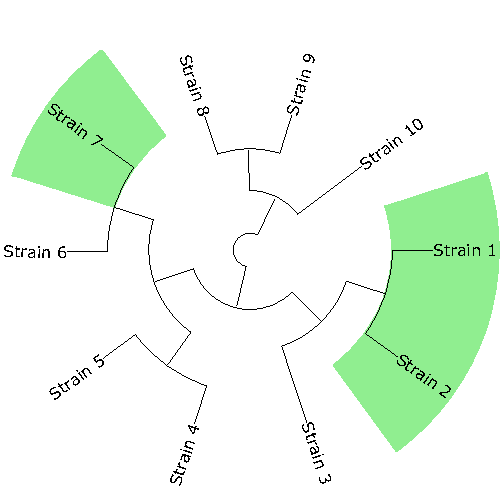
\includegraphics[width=0.9\textwidth]{images/part1/tree_example_1.pdf}
         \caption{Признак с гомоплазией \\(невыпуклый)}
         \label{fig:convex-example-unconvex}
     \end{subfigure}
     \vspace{0.5cm}
     \begin{subfigure}[b]{0.49\textwidth}
         \centering
         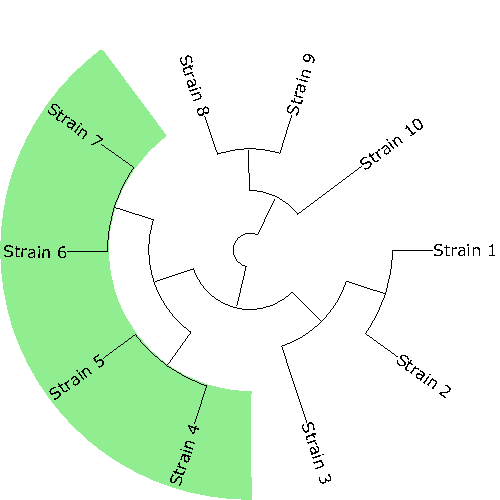
\includegraphics[width=0.9\textwidth]{images/part1/tree_example_2.pdf}
         \caption{Признак, свободный от гомоплазии (выпуклый)}
         \label{fig:convex-example-convex}
     \end{subfigure}
     \caption{Примеры состояния признака на дереве}
     \label{fig:convex-example}
\end{figure}

Более формально: пусть дано множество таксонов $X$ и филогенетическое $X$-дерево $(T, \phi)$, где $T = (V,E)$ — граф, а $\phi: X \rightarrow V$ — отображение, связывающее множество видов с листьями графа.
Признак на множестве таксонов $X$ определяется как функция $\chi$, отображающая некоторое непустое подмножество $X' \subseteq X$ в конечное множество состояний признака $C$:
\[
\chi: X' \rightarrow C.
\]

Признак $\chi$ называется выпуклым на дереве $(T,\phi)$, если существует такая функция расширения признака $\bar{\chi}: V \rightarrow C$, удовлетворяющая следующим условиям:

\begin{enumerate}
    \item $\bar{\chi}(\phi(x)) = \chi(x)$ для всех $x \in X'$, то есть расширение согласовано с исходным распределением признака по листьям;
    \item для каждого состояния признака $\alpha \in C$ индуцированный подграф дерева $T$, образованный вершинами множества $\{ v \in V \mid \bar{\chi}(v) = \alpha \}$, является связным.
\end{enumerate}

Алгоритмически выпуклость признака может быть проверена алгоритмом Фитча.
Этот алгоритм для каждого признака на данном дереве вычисляет минимальное число изменений состояния (0 $\leftrightarrow$ 1, где 1 — признак присутствует) вдоль ветвей, необходимое для воспроизведения наблюдаемого распределения 0/1 на листьях. 
Если минимальное число изменений больше 1, признак не может быть объяснён одним появлением — следовательно, он параллельный.

Важно отметить, что невыпуклость признака может быть следствием как реальных параллельных процессов, так и артефактов (например, неточного построения дерева).
Признак, требующий два изменения, иногда можно сделать выпуклым, чуть изменив топологию дерева.
По этой причине, анализируя параллельные перестройки, следует убедиться в надёжности филогенетической основы и при возможности использовать дополнительные данные (например, информацию о функциях разрываемых регионов), чтобы исключить ложные совпадения.

\subsection{Литературные примеры параллельных изменений}
\label{subsec:parallel_changes_examples}

\begin{figure}[h!]
    \centering
    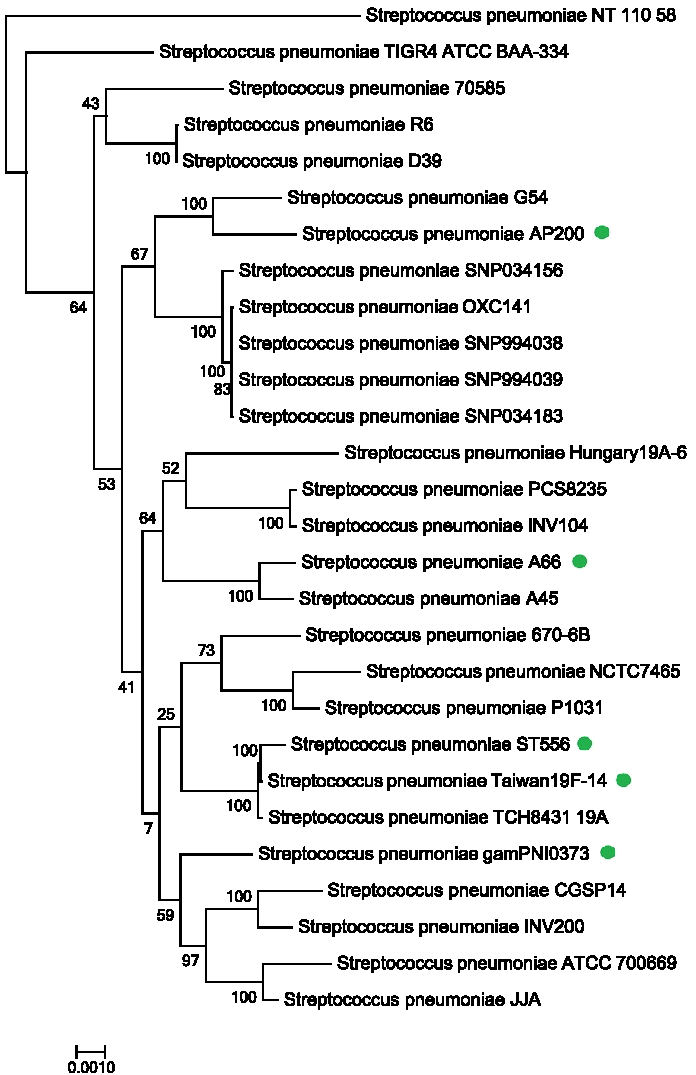
\includegraphics[width=0.55\textwidth]{images/part1/strept-ola-pneu.pdf}
    \caption{Генетическое дерево демонстрирует распределение инверсий по генам PhtD и PhtB, штаммы с такими инверсиями выделены зелёным~\cite{Shelyakin2019}}
    \label{fig:tree-strept}
\end{figure}

Параллельные перестройки геномов наиболее ярко задокументированы у микроорганизмов, где сравнительно небольшие геномы и обилие штаммовых данных позволяют точно отследить независимые события.
Например, в популяциях бактерий \textit{Pseudomonas aeruginosa} наблюдалась инверсия крупного фрагмента хромосомы, фланкированного рибосомными оперонами, которая возникала независимо в разных изолятах~\cite{Irvine2019}.
Показано, что эта перестройка (переворот сегмента между двумя копиями rRNA-гена) приводит к изменениям фенотипа – влиянию на устойчивость к окислительному стрессу, метаболизм и вирулентность; то есть, вероятно, она подвергалась отбору в сходных условиях, возникнув параллельно у разных потомков без недавнего общего предка. 

В работе, посвящённой изучению эволюции стрептококков, выявлены независимые инверсии, связанные с паралогичными генами PhtD и PhtB~\cite{Shelyakin2019}.
Эти перестройки обнаружены у различных штаммов, филогенетически разделённых и не образующих общую кладу по данным генам.
Несмотря на то, что механизм таких инверсий, вероятно, связан с гомологичной рекомбинацией, филогенетический анализ показал, что деревья, построенные на последовательностях генов, задействованных в инверсии, согласуются с общими филогениями этих штаммов, подтверждая независимый характер возникновения событий.
Аналогичные результаты были получены и для других видов рода \textit{Streptococcus}, где параллельные инверсии по указанным паралогам также были выявлены.

Другой пример касается патогенного стрептококка \textit{Streptococcus pyogenes}.
У этого вида обнаружены параллельные изменения числа копий определённых блоков, связанные с фаговыми инсерциями~\cite{Shelyakin2019}.
В частности, блок, содержащий рРНК-оперон, в большинстве геномов представлен несколькими (шестью) копиями, но в некоторых эволюционно удалённых линиях независимо наблюдались либо утраты одной копии, либо, наоборот, приобретение дополнительных копий (до четырёх сверх нормы).
Анализ геномного окружения показал, что эти изменения копийности связаны с независимыми интеграциями и потерями фаговых последовательностей в разных кладах \textit{S.~pyogenes}.
Таким образом, хотя у общего предка всех штаммов было шесть копий оперона, последующие перестройки в различных ветвях привели к разным вариантам — классический случай параллельной эволюции геномной структуры.

Высокие скорости и параллельность перестроек отмечены и в ряде других патогенов.


Хотя большинство исследований параллельных перестроек сосредоточены на прокариотах, аналогичные явления наблюдаются и в эукариотических геномах.
Особенно интересны случаи, в которых крупномасштабные хромосомные инверсии и слияния возникают независимо в различных филогенетических линиях.

Так, в работе~\cite{Porubsky2022} были описаны участки генома человека, демонстрирующие повторяющееся переключение ориентации (англ. \textit{inversion toggling}).
Такие инверсии, возникающие независимо у разных особей, охватывают сотни килобаз и часто обогащены генами.
Интересно, что значительная часть этих регионов совпадает с участками, ранее инвертировавшимися в ходе эволюции приматов, что говорит о древнем и устойчивом характере таких перестроек.

Особый интерес вызывает обнаруженная автором предвзятость по отношению к половым хромосомам: 45\% всех повторяющихся инверсий были локализованы на хромосомах X или Y, что может объясняться особенностями репарации ДНК в непарных участках этих хромосом.
Эти наблюдения подтверждают, что половые хромосомы представляют собой ``горячие точки'' структурной нестабильности, где независимо могут происходить сходные перестройки, включая разрывы и инверсии~\cite{Porubsky2022}.

Стоит отдельно упомянуть гипотезу cети аберрантных филогений, основанная на отборе (англ. \textit{SNAP, Selection-driven Network of Aberrant Phylogenies}), предложенную для объяснения параллельных перестроек~\cite{Brandis2020}.
Согласно этой гипотезе, перестройки могут возникать параллельно под действием сходных селекционных давлений при адаптации к новой нише, особенно если в геноме имеются места, ломкость которых обеспечивает быстрый адаптивный ответ.
Иными словами, сходная среда может ``направлять'' эволюцию разных популяций по похожим структурным путям, вызывая независимые перестройки в аналогичных локусах.
Примеры с инверсиями около rRNA-генов и фаговыми инсерциями в патогенах согласуются с этой идеей, так как соответствующие перестройки дают преимущество в определённых условиях (иммунное уклонение, регуляция вирулентности) и потому появляются в разных линиях независимо.

\subsection{Задача оценки степени параллельности}
\label{subsec:parallelism_estimation}

После выявления параллельных геномных перестроек естественным следующим шагом является количественная оценка степени такого параллелизма.
Понимание, насколько широко распространены независимые повторения структурных изменений, важно для интерпретации их биологического значения и выявления возможных адаптивных механизмов, формирующих эволюцию вида.

В простейшем случае такая оценка может сводиться к подсчёту числа признаков, возникших независимо на разных ветвях филогенетического дерева.
Однако подобный подход не учитывает того, что отдельные события могут повторяться неодинаковое количество раз, и поэтому не всегда отражает истинный масштаб параллельности. 

В связи с этим возникает потребность в более информативных агрегированных показателях, способных учитывать как частоту, так и «силу» повторения перестроек.
Например, таким агрегированным показателем может служить доля параллельных событий от общего числа всех зафиксированных геномных перестроек в данной группе организмов.
Другим примером является индекс гомоплазии, отражающий степень повторности появления одинаковых структурных изменений на эволюционном дереве.
Подобные метрики позволяют дать более глубокое представление о характере и частоте параллельных эволюционных событий и, как следствие, помочь понять их потенциальную адаптивную роль или выявить механизмы структурной нестабильности, присущие определённым геномным регионам.

% \chapter{Расширенный класс моделей демографической истории популяций и методы настройки параметров моделей по генетическим данным}
\label{ch:part2}

В данной главе приведено описание разработанного расширенного класса моделей демографической истории, а также методов настройки параметров моделей по генетическим данным.

Раздел~\ref{sec:part2:new_models} содержит описание моделей расширенного класса, которые могут включать не только непрерывные, но и дискретные параметры динамики изменения численности популяций.

Метод, основанный на комбинации генетического алгоритма и локального поиска, для настройки параметров модели демографической истории по генетическим данным описан в разделе~\ref{sec:part2:genenic_algorithm}.
Гиперпараметры метода были настроены автоматически для эффективного решения поставленной задачи.

В разделе~\ref{sec:part2:bayesian_optimization} представлен метод настройки параметров в условиях сложновычислимой функции, основанный на комбинации ансамблевой байесовской оптимизации и локального поиска.
Разработанный метод имеет настроенные гиперпараметры и эффективен для вывода демографической истории четырех и пяти популяций.

%В разделе~\ref{sec:part2:implementation} приведена информация о реализации разработанных методов.
Разделы~\ref{sec:part2:experiments:genetic_algorithm}~и~\ref{sec:part2:experiments:bayesian_optimization} содержат описание и результаты экспериментальных исследований разработанных методов, основанных на генетическом алгоритме и байесовской оптимизации, для настройки параметров моделей, включая модели расширенного класса.

\section{Расширенный класс моделей демографической истории популяций}
\label{sec:part2:new_models}

Для упрощения работы пользователя-биоинформатика был разработан расширенный класс моделей. 

Эти модели включают новый тип параметров для вывода --- динамики изменения численности.
При этом закон изменения численности в модели теперь может быть не фиксирован, а задан дискретным параметром, и его значение можно найти методом оптимизации.

Приведем пример модели с параметром нового типа. Пусть модель на рисунке~\ref{fig:dadi:model_1} имеет дополнительный параметр \texttt{Dyn} --- динамика изменения второй популяции после разделения.
При разных значениях этого параметра численность второй популяции будет либо константная, либо будет иметь линейный или экспоненциальный закон изменения.
Изображение предложенной модели, а также демографические истории при разных значениях параметра \texttt{Dyn} показаны на рисунке~\ref{fig:new_model:model}.
\begin{figure}[ht]
    \centering
    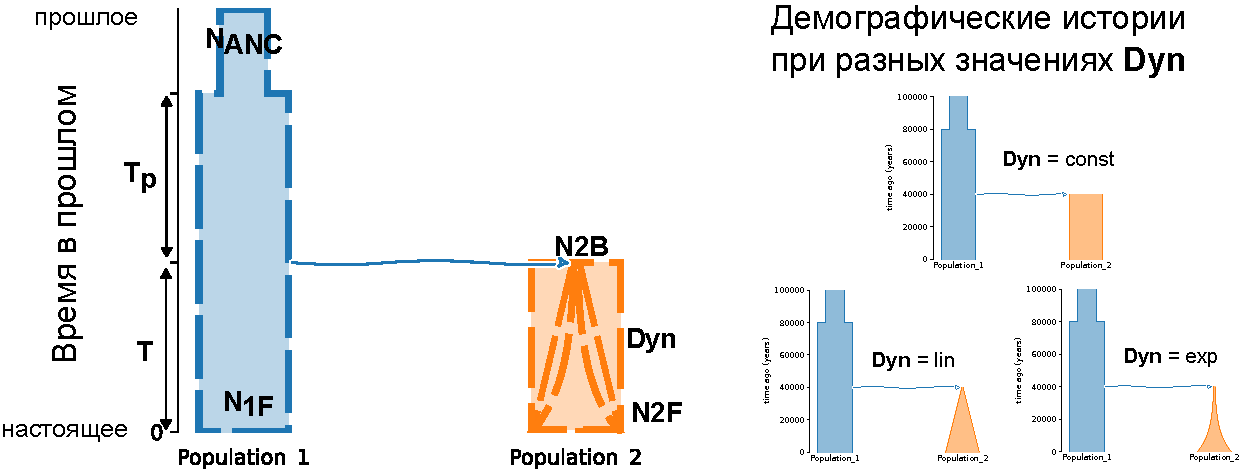
\includegraphics[width=\linewidth]{images_2/picture_2pops_model_3.pdf}
    \caption{Пример разработанной расширенной модели демографической истории с параметрами и соответствующие ей демографические истории при разных значениях параметра \texttt{Dyn}}
    \label{fig:new_model:model}
\end{figure}

В качестве прототипа расширенного класса моделей был выбран первый класс, в котором модели описываются временными интервалами и разделениями популяций.
Этот класс имеет больше преимуществ по сравнению со вторым классом, так как модели в нем могут описывать линейное изменение численности.

\vspace{-0.3cm}
\definition Динамическими характеристиками $\chi_{dyn}(\mathcal{I})$ временного интервала $\mathcal{I} = \langle p, T, \mathfrak{N}^{start}, \mathfrak{N}^{end}, \mathfrak{d} \rangle$ называется множество
$\{d_1, \ldots, d_p\}$, которое соответствует набору динамик временного интервала.

\vspace{-0.3cm}
\definition \textbf{Модель расширенного класса} для демографической истории $P$ популяций --- параметрическая модель для демографической истории $P$ популяций, которая представляется в виде шестерки ${\langle \Theta, \Theta_d, \mathcal{E}, \mathfrak{F}, \mathfrak{F}_{d}\rangle}$, где ${\Theta \subset \mathbb{R}_+^{k_1}}$~---~множество значений непрерывных параметров модели, ${\Theta_d \subset \{0, 1, 2\}^{k_2}}$~---~множество значений дискретных параметров динамики, ${\mathcal{E} = \{E_i\}_{i=1}^K,\ E_i \in \mathcal{I} \cup \mathcal{A} \cup \mathcal{S}}$~---~последовательность элементов временных интервалов, единичных миграций и разделений, ${\mathfrak{F}: \Theta \to  \bigcup \chi(E_i)}$~---~отображение непрерывных параметров модели в характеристики элементов, ${\mathfrak{F}_d: \Theta_d \to  \bigcup \chi_{dyn}(I_i),\ I_i \in \mathcal{E} \cap I}$~---~отображение дискретных параметров динамики в динамические характеристики элементов временных интервалов.

Рисунок~\ref{fig:model_3_type} изображает представление разработанной модели расширенного класса в виде шестерки  $M = \langle\Theta, \Theta_d, \mathcal{E}, \mathfrak{F}, \mathfrak{F}_{d}\rangle$.

\begin{figure}[ht]
    \centering
    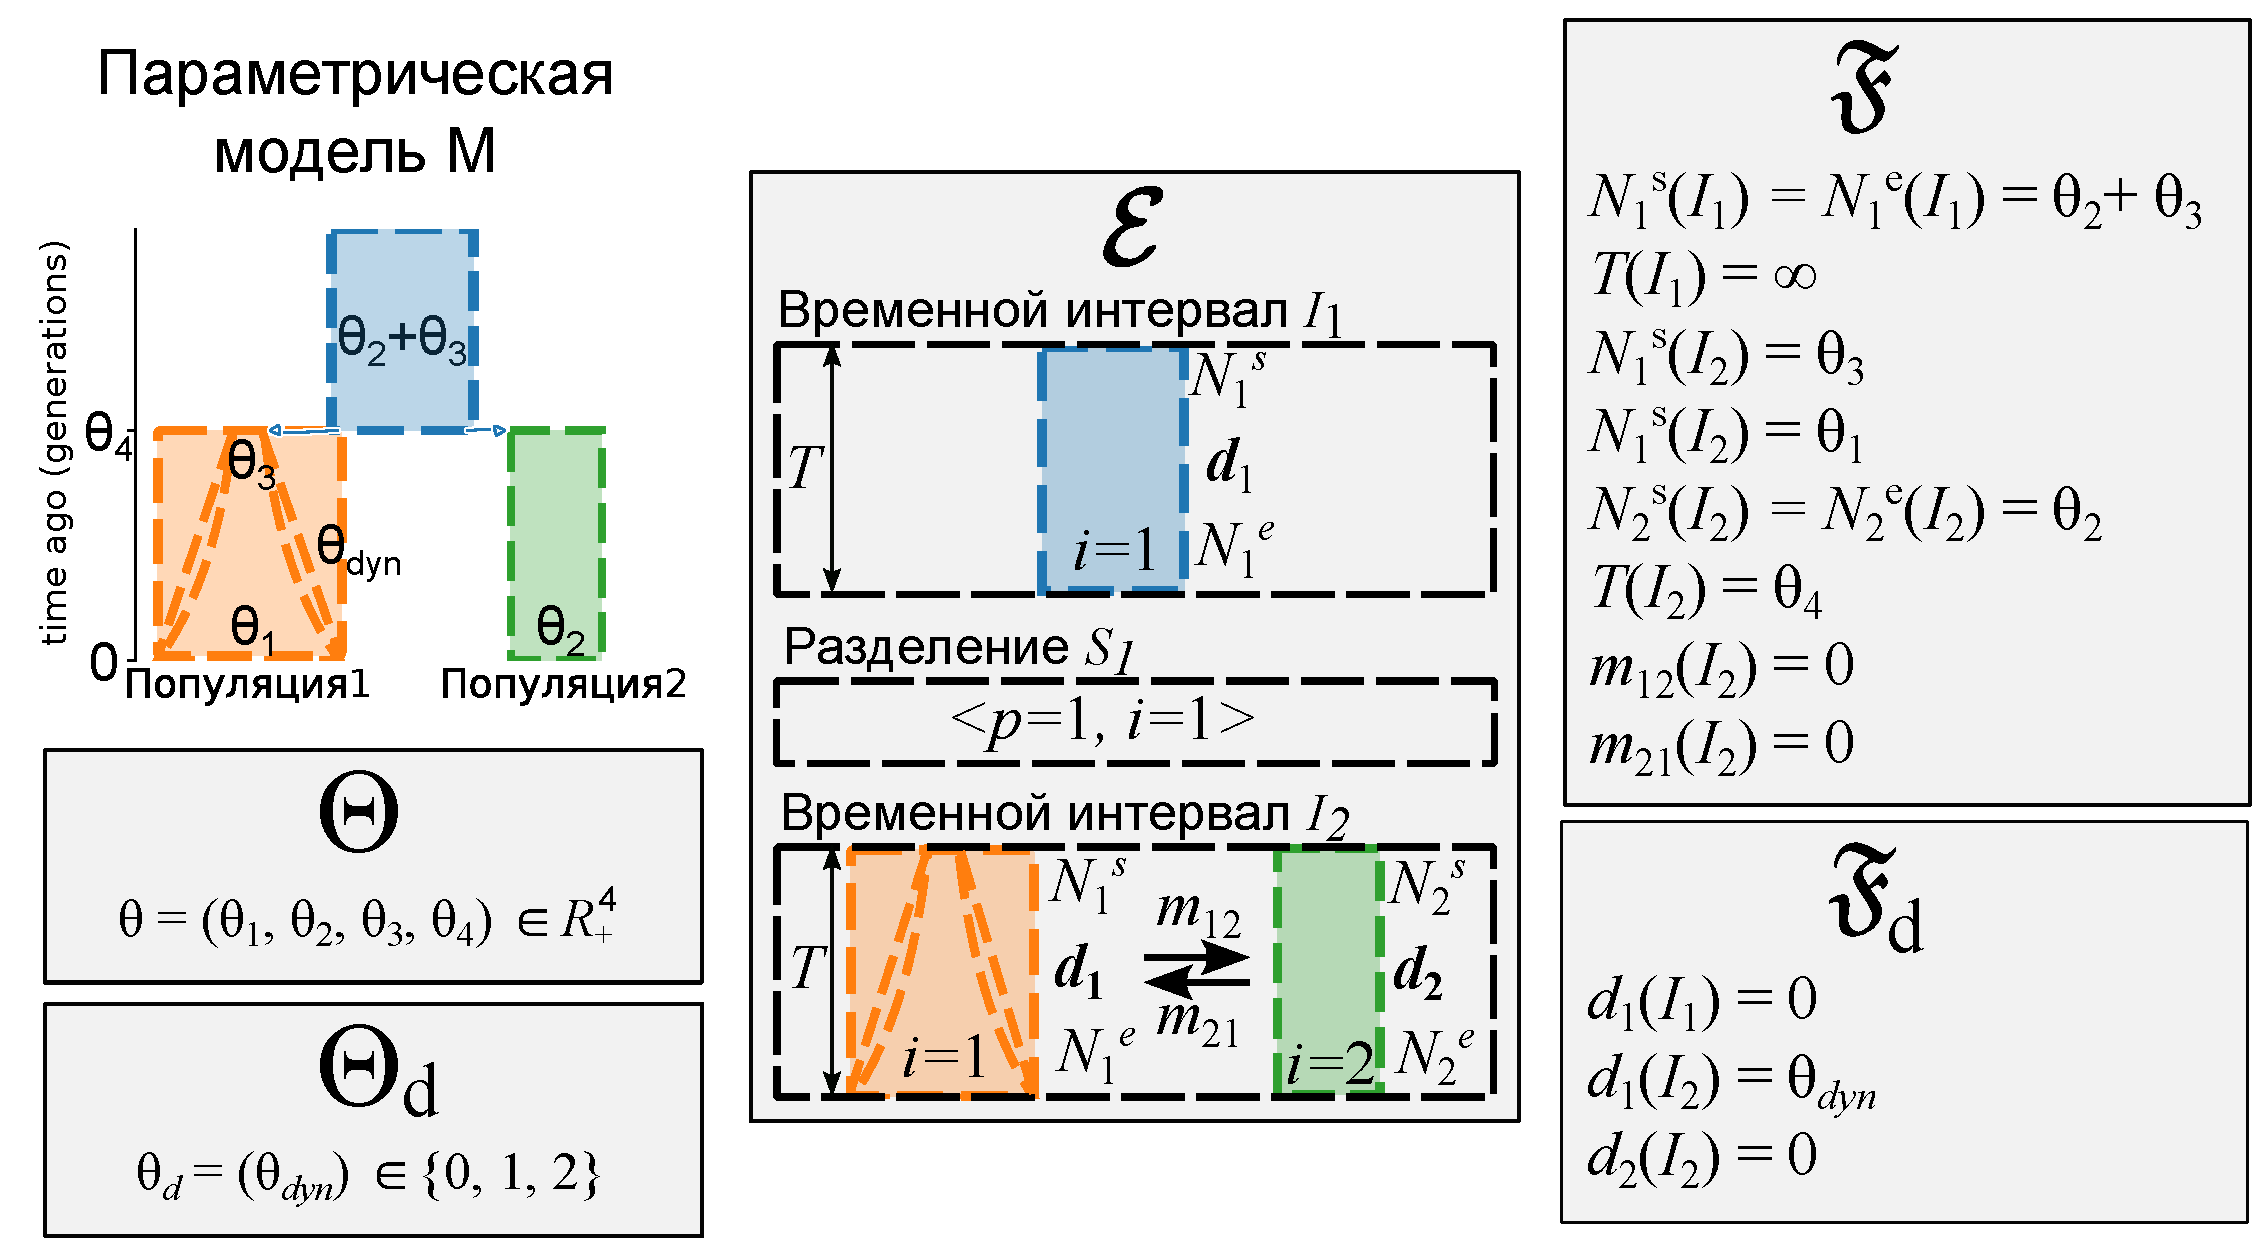
\includegraphics[width=\linewidth]{images_2/model_3_type.pdf}
    \caption{Пример модели $M = \langle\Theta, \Theta_d, \mathcal{E}, \mathfrak{F}, \mathfrak{F}_{d}\rangle$ расширенного класса}
    \label{fig:model_3_type}
\end{figure}

Таким образом, при использовании предлагаемой модели появляется возможность запуска метода оптимизации для определения оптимальных законов изменения численности для любого временного интервала (в нашем примере только для второй популяции). Это позволяет пользователю не перебирать разные модели с разными динамиками вручную, как это требуется для \dadi, \moments, \momentsLD и \momi, а сделать это автоматически.


\textbf{Реализация} моделей расширенного класса была проведена в два этапа.
На первом этапе были спроектированы и реализованы классы для параметров-переменных моделей.
Затем были спроектированы и реализованы классы моделей.
В результате были реализованы два модуля на языке программирования Python: \texttt{variables} и \texttt{models}.

Модуль \texttt{variables} содержит классы параметров моделей.
Структура этих классов представлена на рисунке~\ref{fig:part5:variables_classes}.
Абстрактный класс \texttt{Variable} представляет произвольный параметр с областью определения \texttt{domain} и процедурой \texttt{resample()} генерации случайного значения.
У каждого параметра обязательно присутствует имя \texttt{name}.
От \texttt{Variable} наследуются три абстрактных класса: 1) абстрактный класс \texttt{ContnuousVariable} непрерывных параметров, 2) абстрактный класс \texttt{DiscreteVariable} дискретных параметров, 3) абстрактный класс \texttt{DemographicVariable} параметров моделей демографической истории.
Модуль содержит шесть не абстрактных классов, которые соответствуют следующим параметрам моделей демографической истории:
\begin{itemize}
    \item класс \texttt{PopulationSizeVariable} --- параметры численности популяции;
    \item класс \texttt{TimeVariable} --- параметры времени;
    \item класс \texttt{FractionVariable} --- параметры доли, например, параметр доли особей, совершивших единичную миграцию или параметр доли численности, которая формирует новую популяцию при разделении;
    \item класс \texttt{GrowthRateVariable} --- параметры степени экспоненциального изменения, которые обычно используются в моделях второго класса;
    \item класс \texttt{MigrationVariable} --- параметры темпа непрерывной миграции;
    \item класс \texttt{DynamicVariable} --- параметры динамики изменения численности популяций.
\end{itemize}
Каждый из этих классов является наследником абстрактного класса \texttt{DemographicVariable} и одного из классов \texttt{ContnuousVariable} или \texttt{DiscreteVariable}.


\begin{figure}[ht]
    \centering
    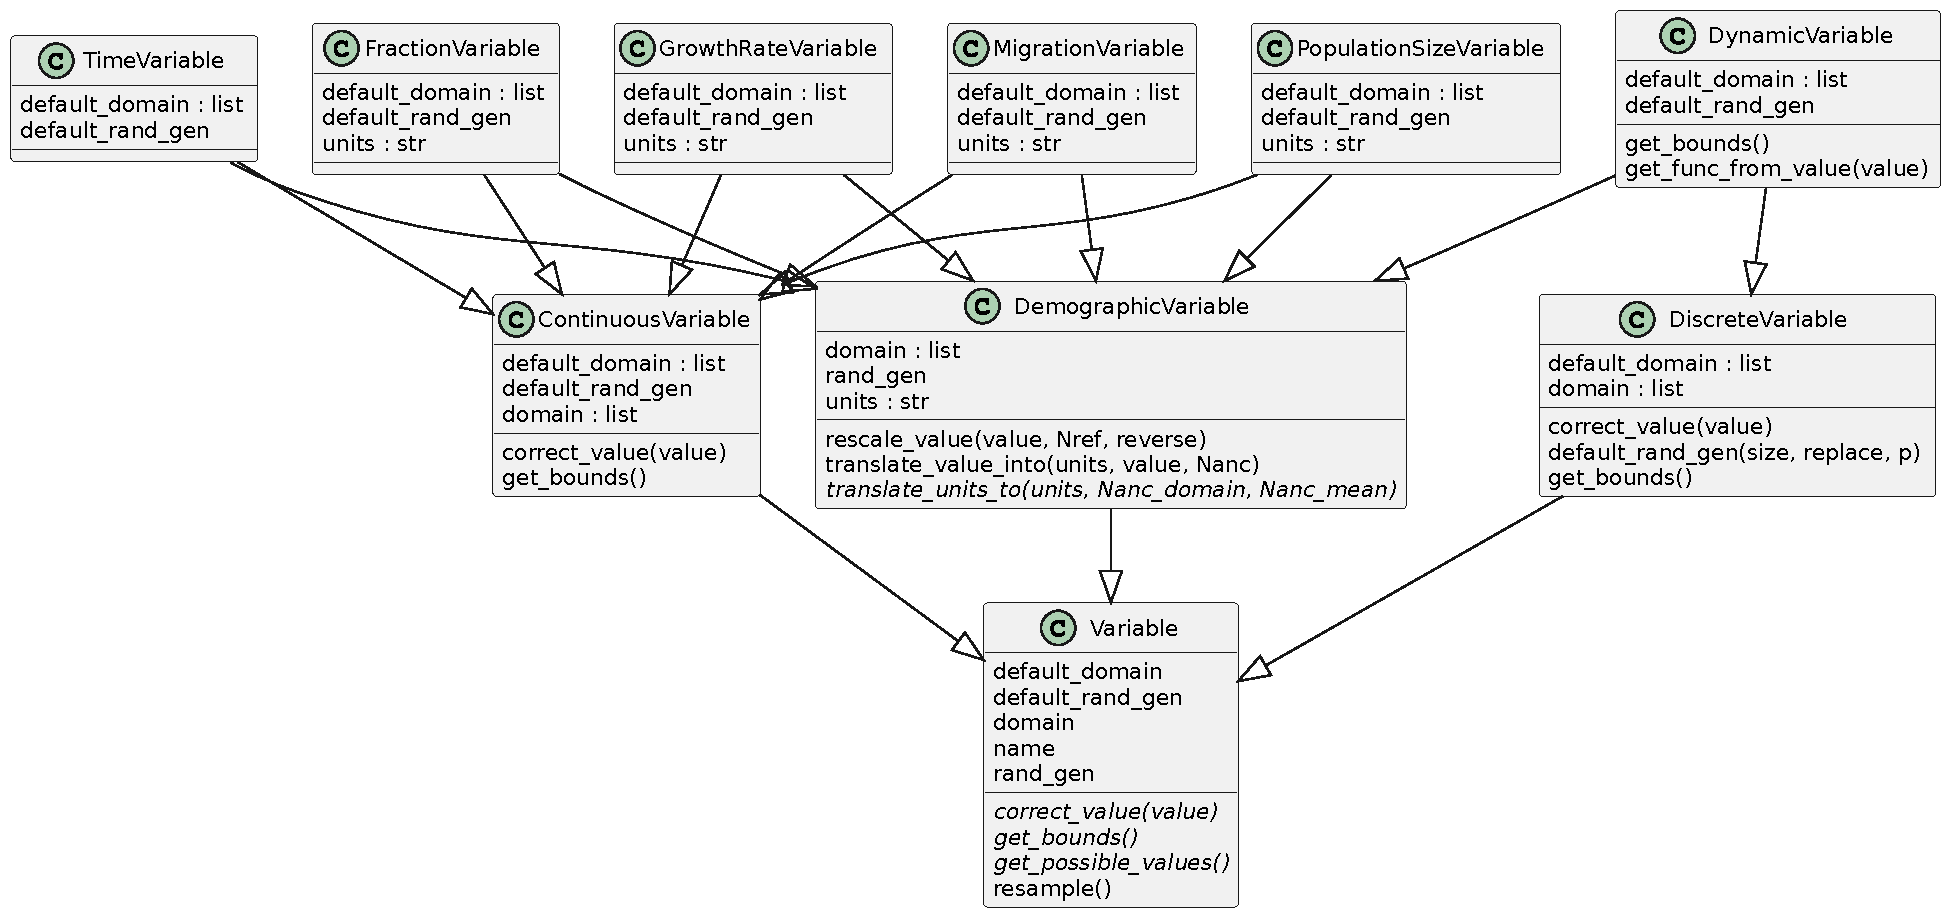
\includegraphics[width=\linewidth]{images/part5/variables_classes.pdf}
    \caption{Структура классов разработанного модуля \texttt{variables}}
    \label{fig:part5:variables_classes}
\end{figure}

Модуль \texttt{models} содержит множество классов для разных моделей.
Структура этих классов представлена на рисунке~\ref{fig:part2:model_classes}.
Основным классом является абстрактный класс \texttt{Model}, который описывает произвольный объект модели с параметрами.
Основными процедурами класса являются процедура \texttt{add\_variable} добавления параметров класса \texttt{Variable} и процедура \texttt{fix\_variable} фиксирования значения указанного параметра.
Можно выделить три группы классов, которые наследуются от \texttt{Model}.

\begin{figure}[ht]
    \centering
    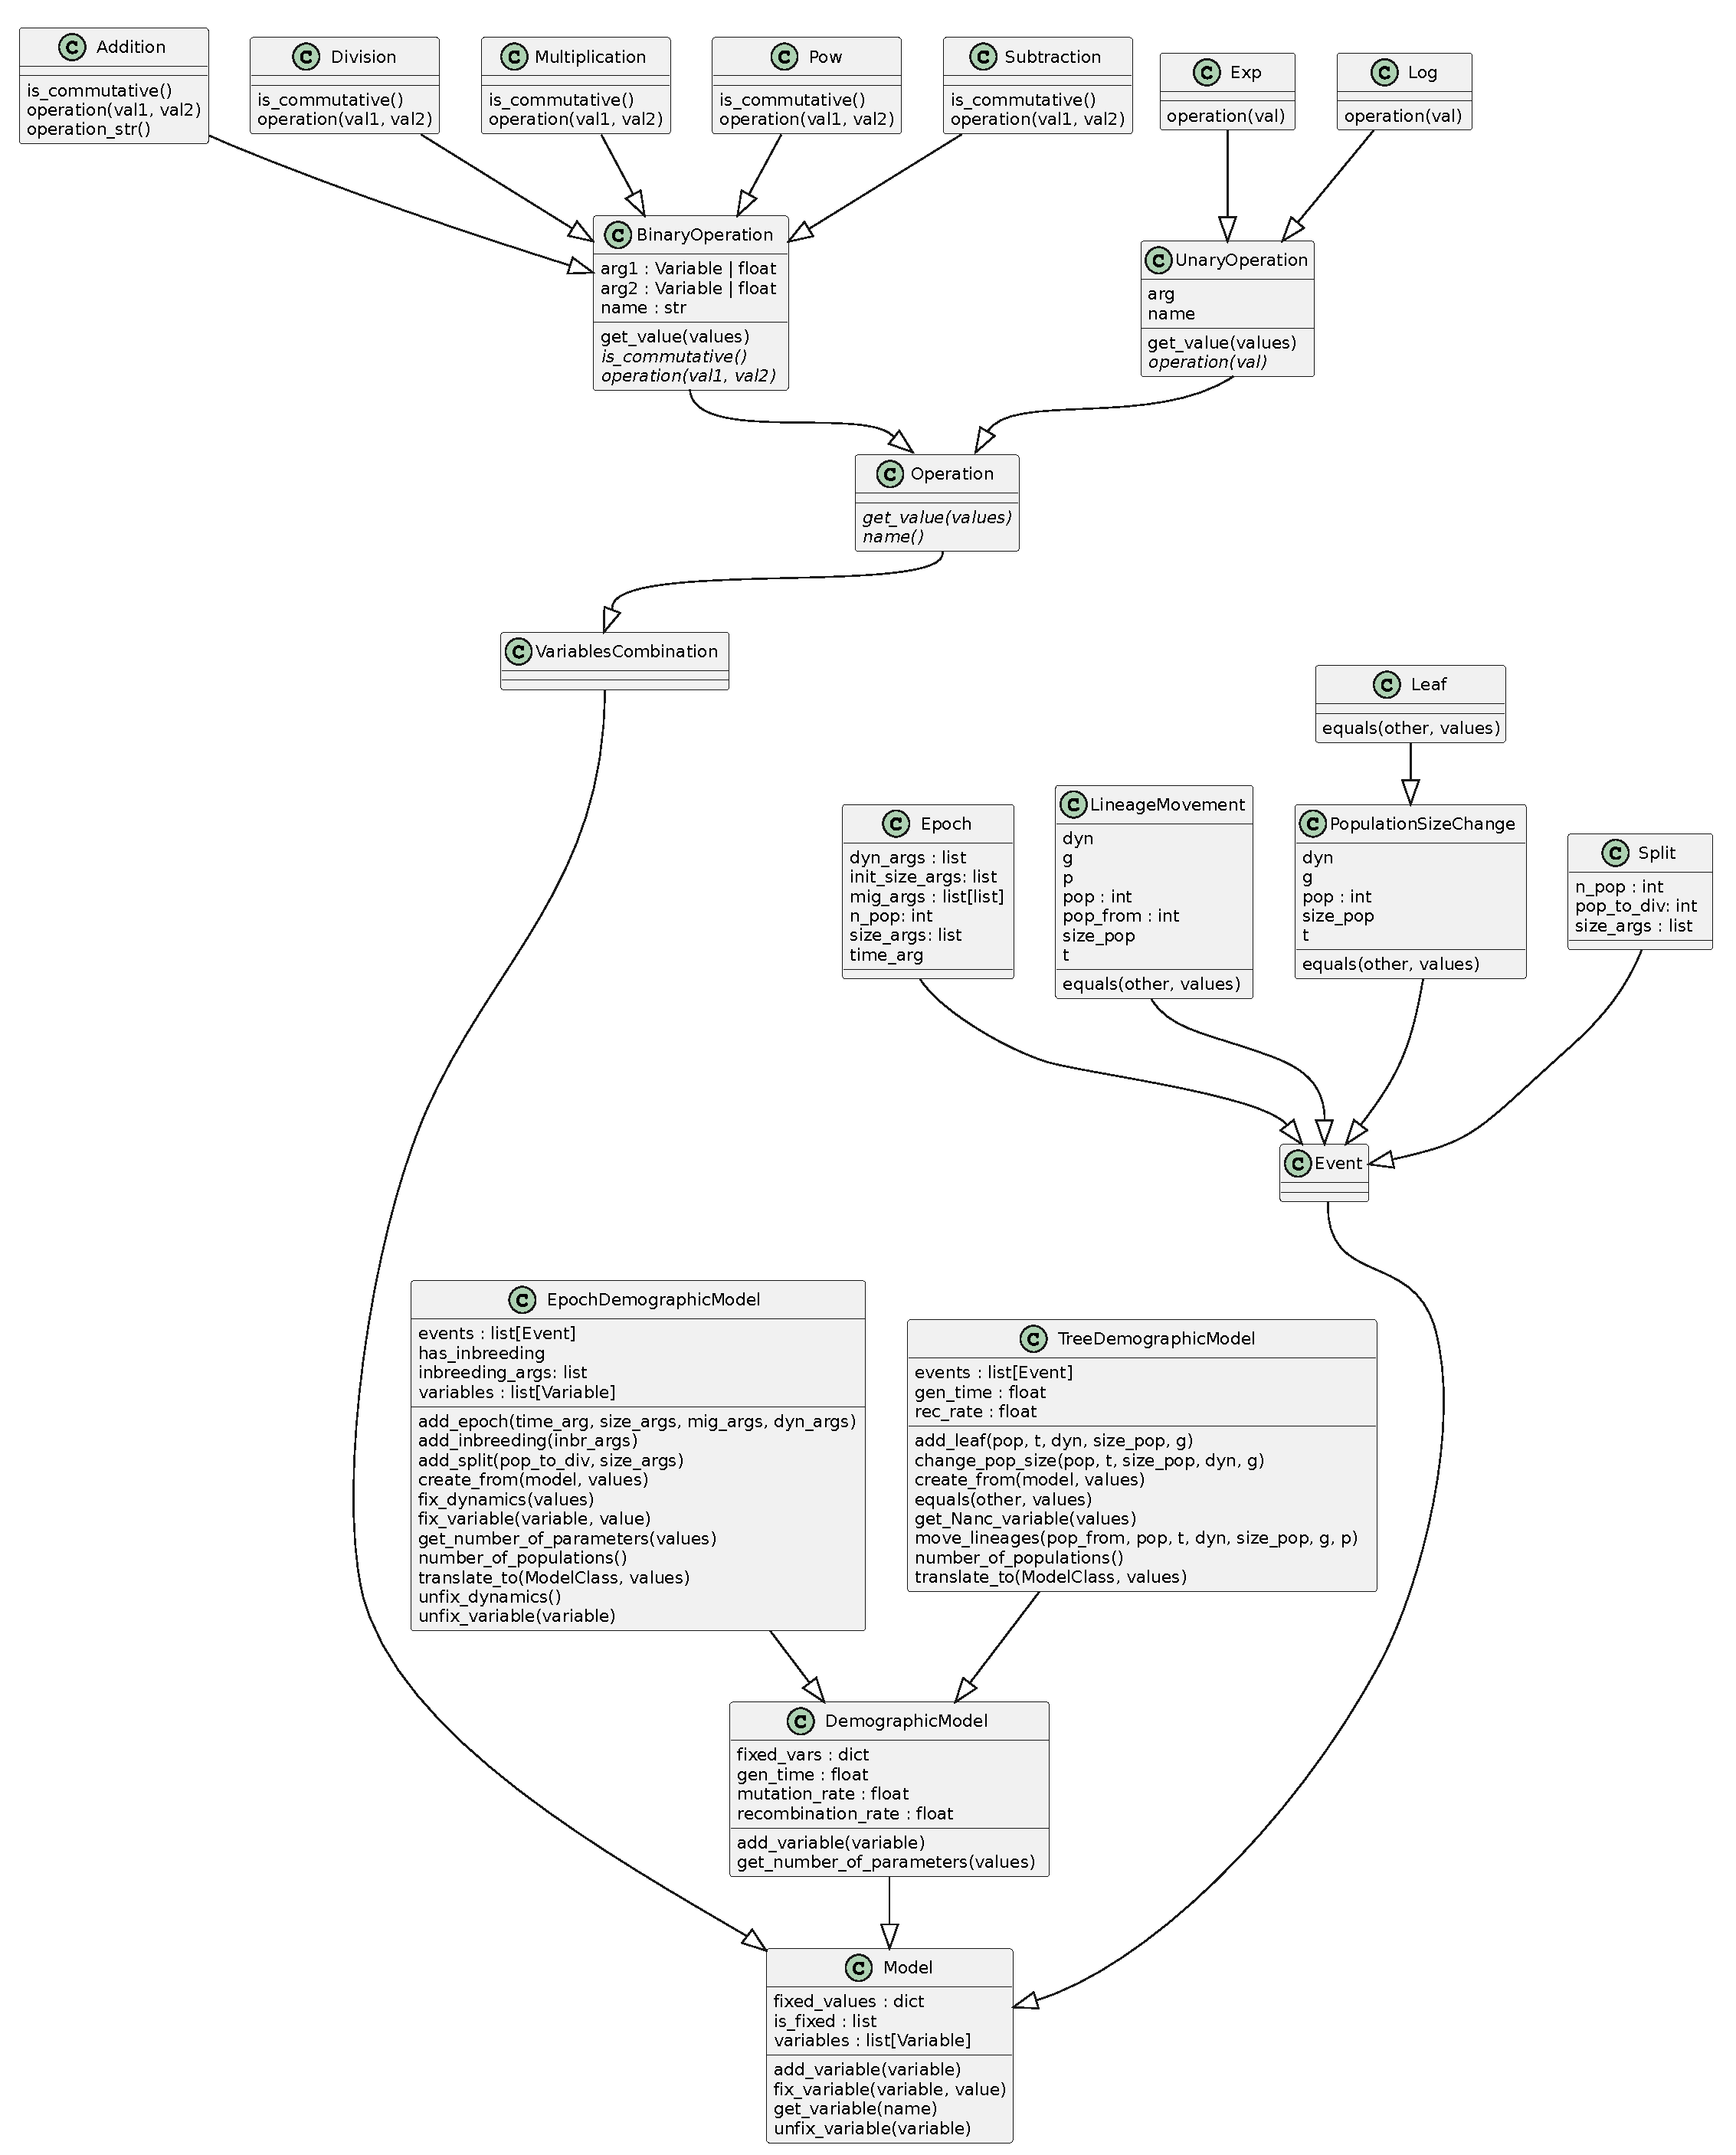
\includegraphics[width=0.97\linewidth]{images/part5/models_part_classes.pdf}
    \caption{Структура классов разработанного модуля \texttt{models}}
    \label{fig:part2:model_classes}
\end{figure}

Первая группа содержит реализацию классов для комбинаций переменных (общий абстрактный класс \texttt{VariablesCombination}).
Он включает в себя бинарные (абстрактный класс \texttt{BinaryOperation}) и унарные (абстрактный класс \texttt{UnaryOperation}) операции для параметров класса \texttt{Variable}.
Среди бинарных операций реализованы операции сложения, деления, умножения, возведения в степень и вычитания параметров.
Были реализованы две унарные операции: логарифмирование параметра и возведение экспоненты в степень параметра.

Вторая группа классов в модуле \texttt{models} --- элементы событий (общий абстрактный класс \texttt{Event}) в моделях демографической истории.
Она включает:
\begin{itemize}
    \item класс \texttt{Epoch}, соответствующий элементам временных интервалов в моделях расширенного класса.
    Он содержит характеристики продолжительности (\texttt{time\_arg}, начальной и конечной численности популяций (\texttt{init\_size\_args} и \texttt{size\_args}), темпов непрерывных миграций (\texttt{mig\_args});
    \item класс \texttt{Split}, соответствующий элементам разделения в моделях расширенного класса;
    \item класс \texttt{PopulationSizeChange}, соответствующий событиям изменения численности в моделях второго класса;
    \item класс \texttt{LineageMovement}, соответствующий событиям единичной миграции в моделях второго класса;
\end{itemize}
Каждая характеристика описанных классов может быть:
\begin{enumerate}
    \item параметром --- объектом класса \texttt{Variable};
    \item комбинацией параметров --- объектом класса \texttt{VariableCombination};
    \item константой --- объектом типа \texttt{str} для характеристик динамики или объектом типа \texttt{float} в случае других характеристик.
\end{enumerate}

Третья группа классов модуля \texttt{models} --- классы моделей демографической истории.
Объекты абстрактного класса \texttt{DemographicModel} содержат основные характеристики рассматриваемых популяций: среднее время одного поколения (\texttt{gen\_time}), вероятность мутации одной позиции генома на одно поколение (\texttt{mutation\_rate}), вероятность рекомбинации позиций генома, находящихся на расстоянии в один миллион пар оснований (\texttt{recombination\_rate}).
У этого класса реализованы два наследника: класс \texttt{EpochDemographicModel} и класс \texttt{TreeDemographicModel}.

Класс \texttt{EpochDemographicModel} \textbf{реализует разработанные модели расширенного класса}.
Заметим, что он также реализует модели первого класса, так как первый класс вложен в расширенный класс моделей.
Объект класса \texttt{EpochDemographicModel} имеет список \texttt{events} элементов временных интервалов --- объекты класса \texttt{Epoch}, и разделений --- объекты класса \texttt{Split}.
Были реализованы четыре основные процедуры: 1) процедура \texttt{add\_epoch} добавления элемента временного интервала, 2) процедура \texttt{add\_split} добавления элемента разделения, 3) процедура \texttt{add\_pulse\_migration} добавления элемента единичной миграции, 4) процедура \texttt{add\_inbreeding} добавления характеристик инбридинга популяций.
Пример задания модели расширенного класса, представленной на рисунке~\ref{fig:new_model:model}, показан на рисунке~\ref{fig:new_model:model_spec}.

\begin{figure}[ht]
    \centering
    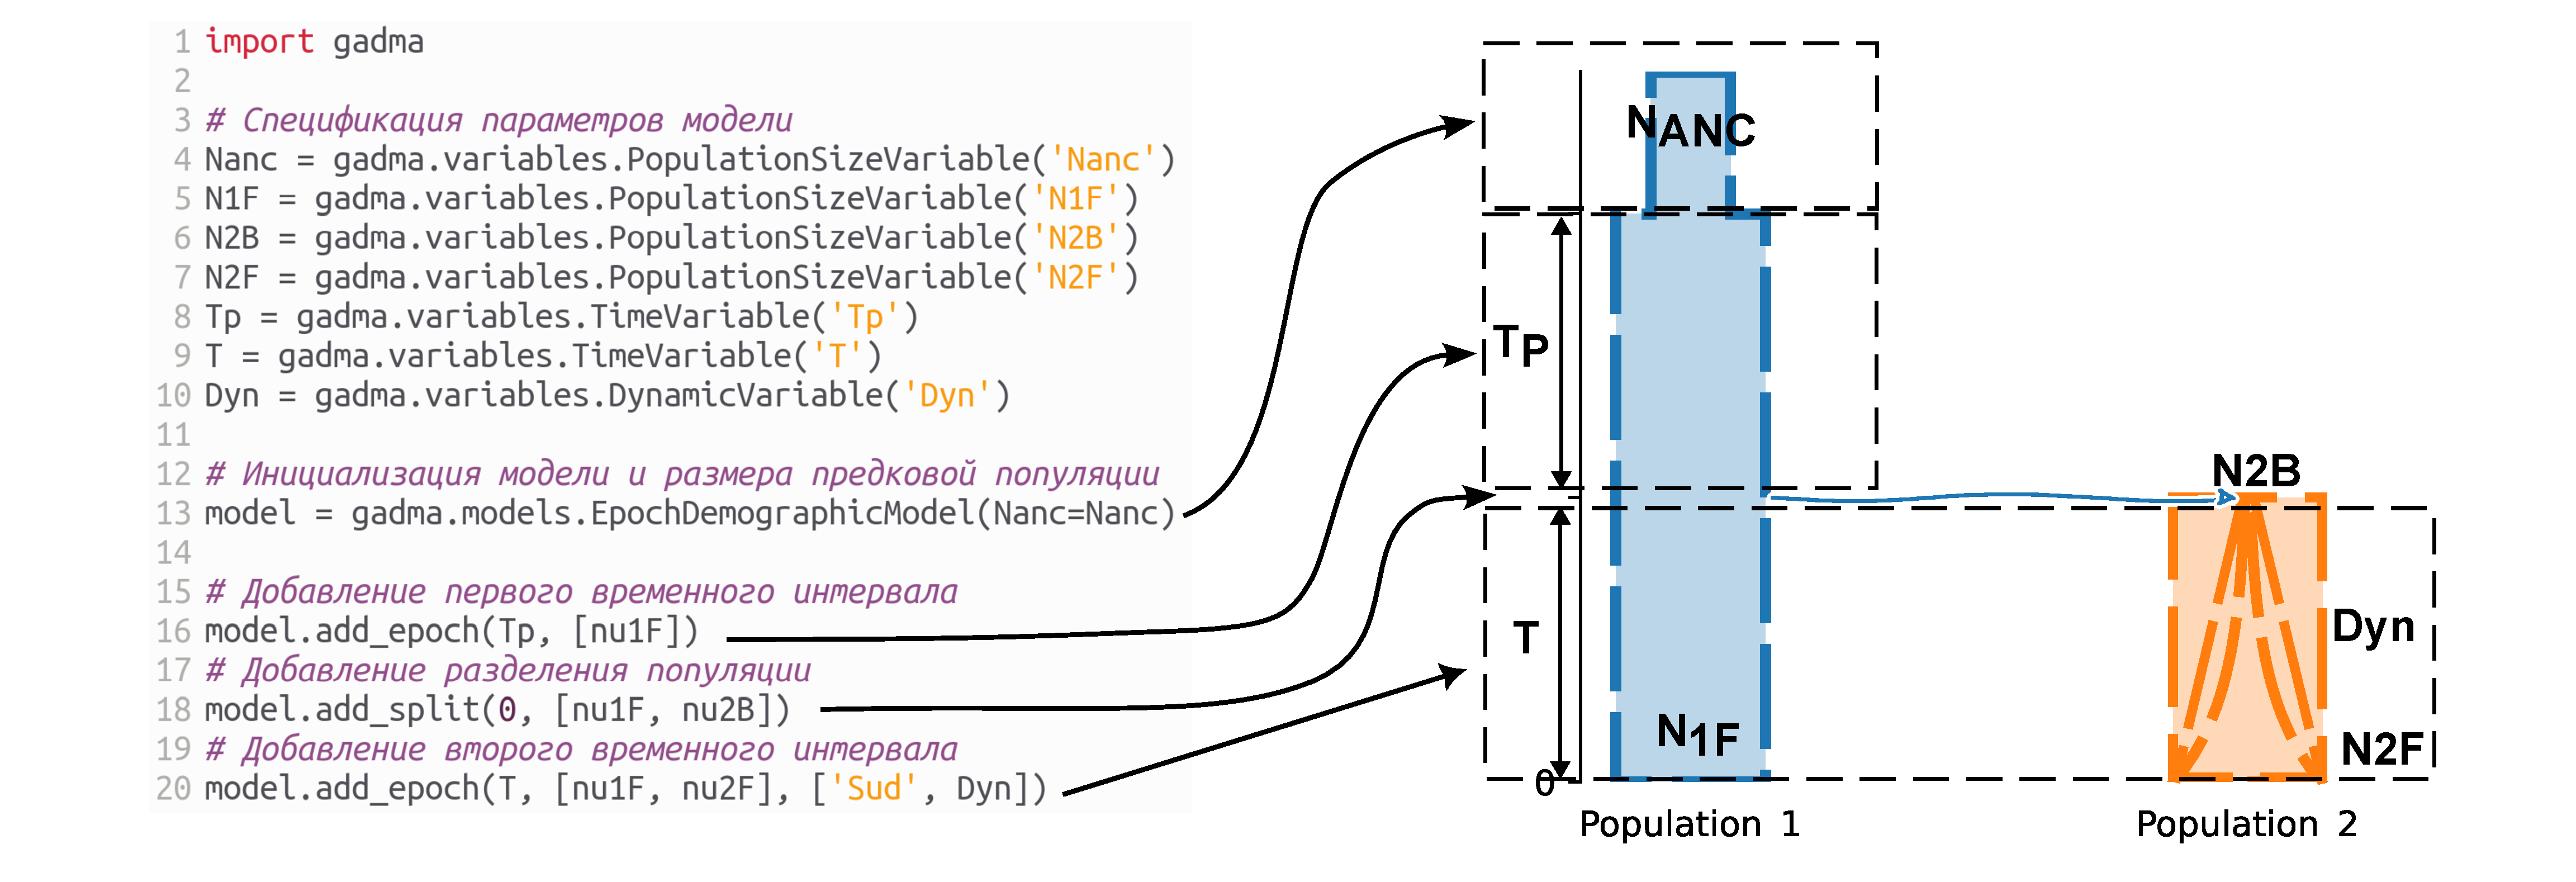
\includegraphics[width=\textwidth]{images_2/gadma_model.pdf}
    \caption{Пример задания расширенной модели}
    \label{fig:new_model:model_spec}
\end{figure}

Класс \texttt{TreeDemographicModel} реализует модели второго класса.
Он содержит список \texttt{events} событий изменения численности --- объектов класса \texttt{PopulationSplit}, и событий единичной миграции --- объектов класса \texttt{LineageMovement}.

Классы \texttt{EpochDemographicModel} и \texttt{TreeDemographicModel} были реализованы вместе с процедурой \texttt{translate\_to}, которая переводит модель из одного класса в другой при заданных значениях параметров.
Таким образом, реализованную модель расширенного класса при фиксированных значениях параметров можно перевести в модель второго класса для использования в библиотеке \momi.



\FloatBarrier
\section{Метод на основе комбинации генетического алгоритма и локального поиска для настройки параметров моделей демографической истории популяций по генетическим данным}
\label{sec:part2:genenic_algorithm}

\emph{Эволюционные алгоритмы} --- это класс алгоритмов оптимизации, основанных на биологической эволюции и ее принципах.
Они используют процессы, которые происходят в природе, такие как мутация, скрещивание и естественный отбор, для решения задач оптимизации.

Один из наиболее известных и широко используемых эволюционных алгоритмов --- \emph{генетический алгоритм}~\cite{holland1975adaptation}. 
Он моделирует процесс естественного отбора в биологии и применяется для поиска наилучшего решения в пространстве поиска.
Генетический алгоритм начинается с определения первого \emph{поколения} $X^{\text{init}}$ размера $N_\text{gen}$, которое состоит из $N_\text{gen}$ \emph{особей}, представляющих потенциальные решения задачи.
Каждая особь в генетическом алгоритме представляет собой вектор $x_i = (x_{i, 1}, \cdots, x_{i, N})$ параметров целевой функции $f$, и этот вектор $x_i$ называется геномом.
Каждый параметр $x_{i, j}$ этого вектора --- ген, и он соответствует определенной характеристике решения, которую нужно оптимизировать.
Первое поколение $X^{\text{init}} = \{x^0_i\}_{i=1}^K$ особей в генетическом алгоритме может быть сгенерировано случайным образом.
Затем происходит итерационный процесс, в котором каждое новое поколение $X_t$ создается на основе предыдущего $X_{t-1}$, используя операторы генетических операций таких как мутация, скрещивание и отбор.

Оператор \emph{мутации} в генетическом алгоритме --- это случайное изменение генов особи (решения) с некоторой вероятностью.
Мутация может произойти в любом месте генома особи, и это может привести к изменению соответствующей характеристики решения.
Существует несколько способов реализации мутации в генетическом алгоритме, но наиболее распространенный --- это замена значения случайно выбранного гена $x_{i, j}$ на другое случайно выбранное значение из допустимого диапазона.
Оператор \emph{скрещивания} в генетическом алгоритме представляет собой процесс создания новых особей путем комбинирования генетического материала двух родительских особей.
Самый простой и широко используемый вид скрещивания --- это одноточечное скрещивание (single-point crossover), когда случайно выбирается точка раздела между генами в родительских геномах, и гены до этой точки копируются из первого родителя, а после этой точки --- из второго.
Другой вид скрещивания --- равномерное (uniform), обозначает выбор каждого гена равновероятно между соответствующими генами родителей.
Процесс \emph{отбора} в генетическом алгоритме заключается в выборе наиболее приспособленных особей для создания следующего поколения.
Особи оцениваются по значению \emph{функции приспособленности} (fitness), которая отражает качество решения, представленного данным геномом.
Часто значение приспособленности определяется целевой функцией $f$.
В результате каждой итерации, находится новое поколение решений, которое более близко к оптимальному решению.

Генетический алгоритм применяется для решения различных задач биоинформатики, например, для поиска генов и аннотации генома~\cite{chowdhury2017optimized}, выравнивания нескольких последовательностей~\cite{chowdhury2017review}, моделирования структуры белков~\cite{unger2004genetic}, поиска новых молекул лекарств~\cite{spiegel2020autogrow4} и многого другого. 

Также существуют методы, которые сочетают в себе несколько различных подходов, они называются \emph{комбинированными методами оптимизации}.
Например, генетический алгоритм может быть применен в сочетании с методом локального поиска для улучшения точности оптимизации.
В работе~\cite{yang2016genetic} такой комбинированный метод был разработан для поиска связей между мутациями в генах и болезнями.

\subsection{Разработка метода на основе комбинации генетического алгоритма и локального поиска}

В этом разделе описан разработанный метод для настройки параметров модели демографической истории популяций по генетическим данным.

Это комбинированный метод, основанный на совместном использовании генетического алгоритма и метода локальной оптимизации, для решения задачи настройки параметров $\theta$ модели $\mathcal{M}$ демографической истории популяций по генетическим данным.
Метод представляет последовательный запуск генетического алгоритма и метода локальной оптимизации. 
Генетический алгоритм был модифицирован для оптимизации как непрерывных параметров целевой функции, так и дискретных, что позволяет применять его для настройки параметров разработанных моделей расширенного класса.
В качестве методов локальной оптимизации в разработанном комбинированном методе предлагается применять методы BFGS, L-BFGS-B, Пауэлла или Нелдера-Мида, которые используются в существующих методах настройки параметров моделей первого и второго класса~\cite{gutenkunst2009inferring, }.
Эти методы позволяют настраивать только непрерывные параметры, поэтому при их применении значения дискретных параметров моделей расширенного класса фиксируются.
Таким образом, разработанный комбинированный метод, основанный на генетическом алгоритме, сначала производит настройку всех параметров заданной модели с использованием генетического алгоритма, а затем проводит дополнительную настройку непрерывных параметров с помощью выбранного метода локальной оптимизации.

Приведем подробное описание примененного генетического алгоритма.
Описание рассматриваемых методов локальной оптимизации было дано ранее в разделе~\ref{sec:part1:dem_inf:opt_methods}.

Геномом особи в генетическом алгоритме является вектор значений параметров $\theta$ заданной модели $\mathcal{M}$, а функция приспособленности равна целевой функцией $f_\mathcal{M}(\theta)$, которая является логарифмом правдоподобия $\log (\mathcal {L} (\theta | \mathfrak{D}))$.
%Используется отрицательное значение, так как решается задача минимизации.

На первом этапе генетический алгоритм генерирует поколение особей, случайным образом, если оно не было задано заранее.
Для формирования нового поколения отбираются наиболее приспособленные особи --- с наибольшими значениями функции приспособленности, среди набора мутировавших, скрещенных и случайных особей.
Выбор особей для применения операторов мутации или кроссовера является случайным, но вероятность выбора прямо пропорциональна значению приспособленности: чем лучше приспособленность вектора параметров, тем больше вероятность того, что он будет выбран.
Генетический алгоритм останавливается, когда он больше не может получить лучшее решение по значению функции приспособленности за несколько итераций.

Схема алгоритма метода, основанного на комбинации генетического алгоритма и локального поиска, представлена на рисунке~\ref{fig:part2:genetic_algorithm}.

\begin{figure}[ht]
  \centering
   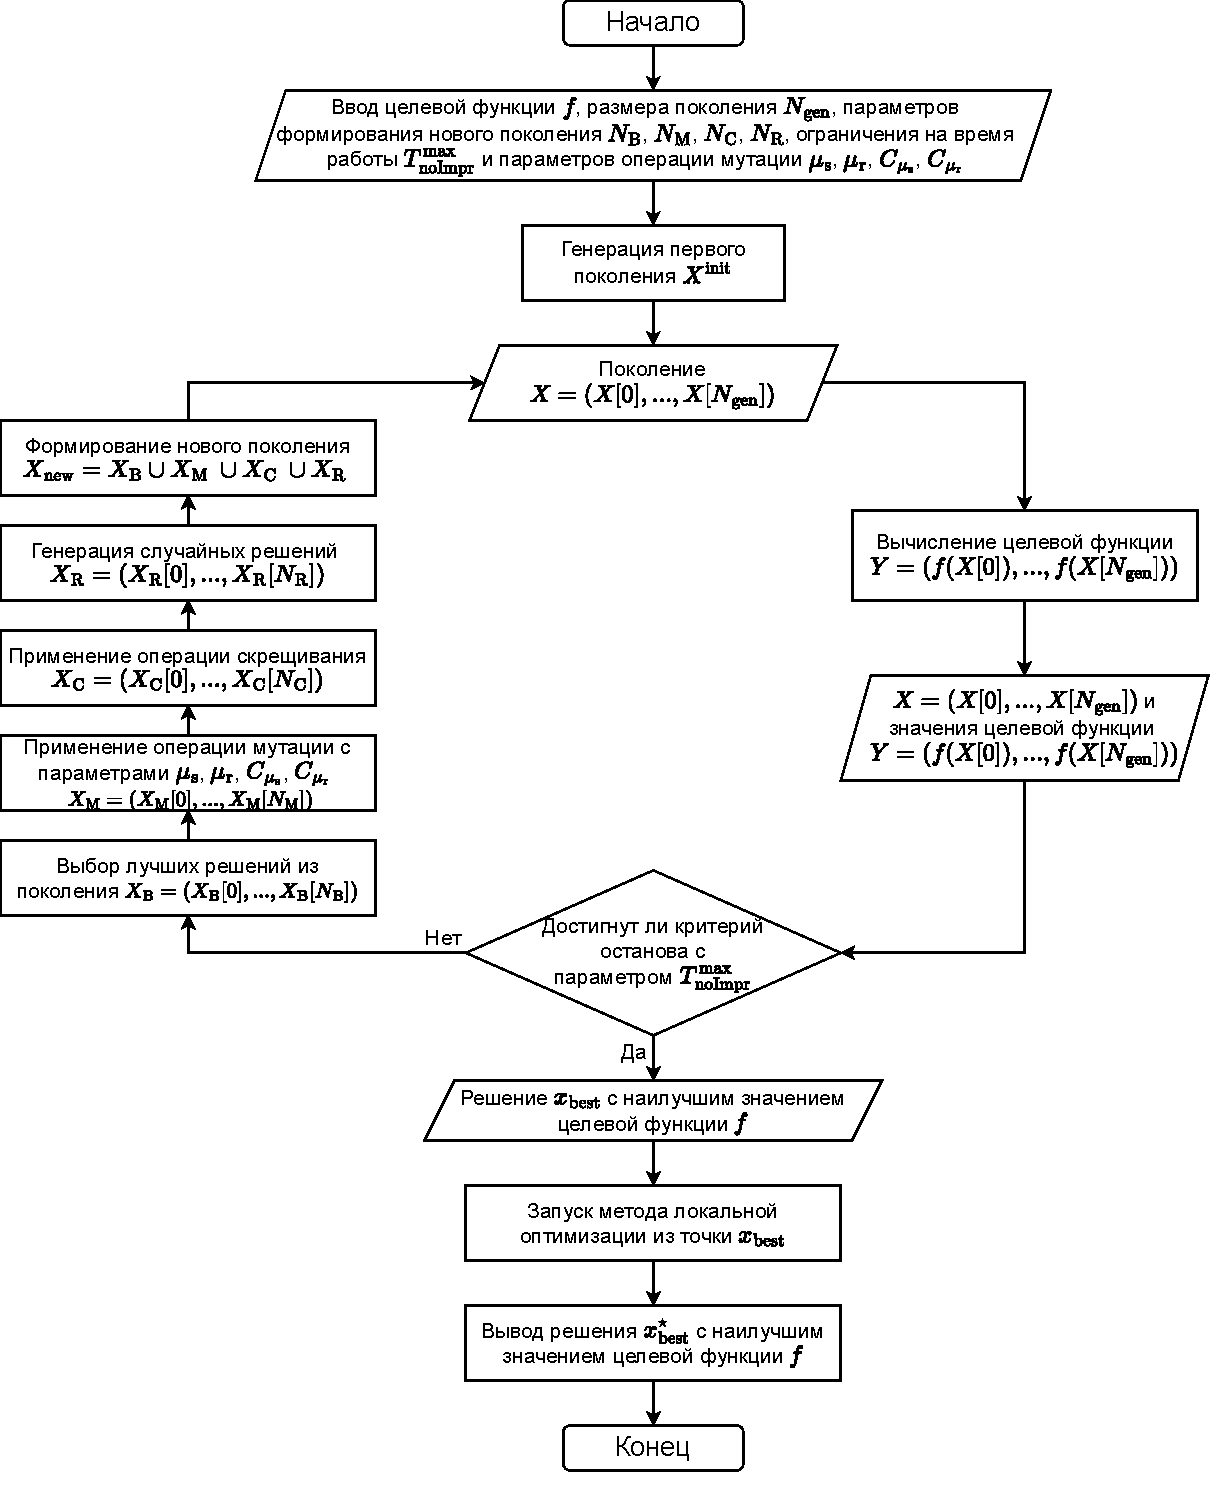
\includegraphics[width=\linewidth]{images/part2/genetics_algorithm/genetic_algorithm_scheme.drawio.pdf}
   \caption{Схема алгоритма метода, основанного на комбинации генетического алгоритма и локального поиска}
  \label{fig:part2:genetic_algorithm}
\end{figure}



Псевдокод разработанного генетического алгоритма представлен в листинге~\ref{alg:part2:genetic_algorithm}.
На вход алгоритм принимает следующие параметры: целевая функция $f$, начальный набор решений $X^{\text{init}}$, число лучших решений $N_{\text{E}}$ предыдущего поколения в новом, число мутировавших решений $N_{\text{M}}$, число потомков скрещенных решений $N_\text{C}$, число случайно-сгенерированных решений $N_\text{R}$ в новом поколении, максимальное число итераций без улучшения $T_{\text{noImpr}}^{\max}$, сила миграции $\mu_\text{s}$, степень миграции $\mu_\text{r}$ и константы $C_{\mu_\text{s}}, C_{\mu_\text{r}}$, определяющие их изменения.

\begin{algorithm}[ht]
\caption{Псевдокод разработанного генетического алгоритма}
\label{alg:part2:genetic_algorithm}
\begin{algorithmic}[1]
\Function{GeneticAlgorithm}{$f, X^{\text{init}}, N_{\text{E}}, N_{\text{M}}, N_{\text{C}}, N_{\text{R}},  T_{\text{noImpr}}^{\max}, \mu_\text{s}, \mu_\text{r}, C_{\mu_\text{s}}, C_{\mu_\text{r}}$}
\State $N_{\text{gen}}  \leftarrow (N_\text{B} + N_\text{M} + N_\text{C} + N_\text{R})$ \Comment{Размер поколения}
\State {$Y^{\text{init}} \leftarrow \{f(\theta), \theta \in X^{\text{init}}\}$}
\State $X, Y \leftarrow$ \Call{Selection}{$X^{\text{init}}, Y^{\text{init}}, N_{\text{gen}}$} \Comment{$\text{Первое поколение решений}$}
\State $T_{\text{noImpr}} \leftarrow 0$ \Comment{$\text{Счетчик числа итераций без улучшения}$}
\While {$T_{\text{noImpr}} \leq T_{\text{noImpr}}^{\max}$}
    \State $X_{\text{new}}  \leftarrow  [\ ]$ \Comment{$\text{Строим новое поколение решений}$}
    \State $\omega \leftarrow \left\{\frac{Y[i]}{\sum_j Y[j]}\right\}_{i=1}^{N_{\text{gen}}}$ \Comment{$\text{Вероятности выбора решений}$}
    \For{$l \leftarrow 1..N_\text{B}$} \Comment{$\text{Добавляем лучшие модели}$}
        \State $X_{\text{new}}.$\Call{Add}{$X[l]$}
    \EndFor
    \For{$l \leftarrow 1..N_\text{M}$} \Comment{$\text{Добавляем мутированные решения}$}
        \State $j \leftarrow$ \Call{DiscreteRandom}{$\{i\}_{i=1}^N, \omega$}
        \State $X_{\text{new}}.$\Call{Add}{\Call{Mutate}{$X[j], \mu_\text{s}, \mu_\text{r}$}}
    \EndFor
    \For{$l \leftarrow 1..N_\text{C}$} \Comment{$\text{Добавляем скрещенные решения}$}
        \State $j_1 \leftarrow$ \Call{DiscreteRandom}{$\{i\}_{i=1}^N, \omega$}
        \State $j_2 \leftarrow$ \Call{DiscreteRandom}{$\{i\}_{i=1}^N, \omega$}
        \State $X_{\text{new}}.$\Call{Add}{\Call{CrossOver}{$X[j_1], X[j_2]$}}
    \EndFor
    \For{$k \leftarrow 1..N_\text{R}$}  \Comment{$\text{Добавляем случайные решения}$}
        \State{$X_{\text{new}}.$\Call{Add}{\Call{GenerateRandomParameters}{$\,$}}}
    \EndFor
    \State {$Y^{\text{new}} \leftarrow \{f(x), x \in X^{\text{new}}\}$}
    \State $X_{\text{new}} \leftarrow $\Call{Selection}{$X_{\text{new}}, Y_{\text{new}}, N_{\text{gen}}$}
    \If {$f(X_{\text{new}}[0]) > f(X[0])$}  \Comment{$\text{Обновление счетчика}$}
        \State $T_{\text{noImpr}}  \leftarrow 0$
        \State $b_{\text{improved}} \leftarrow \text{True}$
        \State $b_{\text{improvedByMutation}} \leftarrow (X_{\text{new}}[0].\text{lastOperation} == \text{\texttt{"Mutation"}})$

    \Else
        \State $T_{\text{noImpr}} \leftarrow T_{\text{noImpr}} + 1$
        \State $b_{\text{improved}} \leftarrow \text{False}$ 
        \State $b_{\text{improvedByMutation}} \leftarrow \text{False}$
    \EndIf
    \State $X \leftarrow X_{\text{new}},\ Y \leftarrow Y_{\text{new}}$
    \State \Comment{Обновление адаптивной силы и степени мутации\hfill}
    \State $\mu_\text{s} \leftarrow \Call{UpdateValue}{b_{\text{improvedByMutation}}, \mu_\text{s}, C_{\mu_\text{s}}}$ 
    \State $\mu_\text{r} \leftarrow \Call{UpdateValue}{b_{\text{improved}}, \mu_\text{r}, C_{\mu_\text{r}}}$ %\Comment{Адаптивная степень мутации}
\EndWhile
\State \Return $X[0]$
\EndFunction
\end{algorithmic}
\end{algorithm}

\FloatBarrier

\textbf{Мутация} особи в генетическом алгоритме равнозначна процессу изменения значений отдельных генов.
На рисунке~\ref{fig:part2:mutation} показано применение операции мутации для изменения одного гена --- параметра заданной модели демографической истории.
Разработанный оператор определяется двумя константами: \textit{силой} $\mu_{s}$ и \textit{степенью} $\mu_{r}$ мутации.
Число изменяемых генов-параметров выбирается из биномиального распределения $\sim B(n, \mu_{s})$ со средним значением, равным силе мутации.
Гены, которые мутируют, выбираются с вероятностью, прямо пропорциональной их весам $\omega$, которые вначале равны --- выбор равновероятен, а затем каждый вес может быть увеличен, если произошла мутация соответствующего гена, которая привела к улучшению модели.

Разработанный генетический алгоритм позволяет работать как с непрерывными параметрами, так и с дискретными.
При мутации гена, который соответствует непрерывному параметру, мера того насколько его значение изменится определяется знаком: $-1$ или +1 равновероятно, и абсолютной мерой $\lambda$, которая случайным образом генерируется из усеченного на отрезке $[0, 1]$ нормального распределения $\lambda \sim \hat{N}(\mu_r, \sigma^2, 0, 1)$ со средним значением, равным силе мутаций и дисперсией $\sigma^2$.
Дисперсия $\sigma^2$ определяется специальной процедурой $\text{SigmaBasedOnThreeSigmaRule}$, описание которой приведено далее.% в разделе~\ref{sec:part2:genetic_algorithm:3_sigma_rule}.
Если происходит мутация гена, который соответствует дискретному параметру, то его значение изменяется равновероятно на любое другое возможное.
Псевдокод для процедуры мутации разработанного генетического алгоритма в случае, когда параметры модели непрерывны, представлен в листинге~\ref{alg:part2:mutation}.

\begin{figure}[ht]
  \centering
  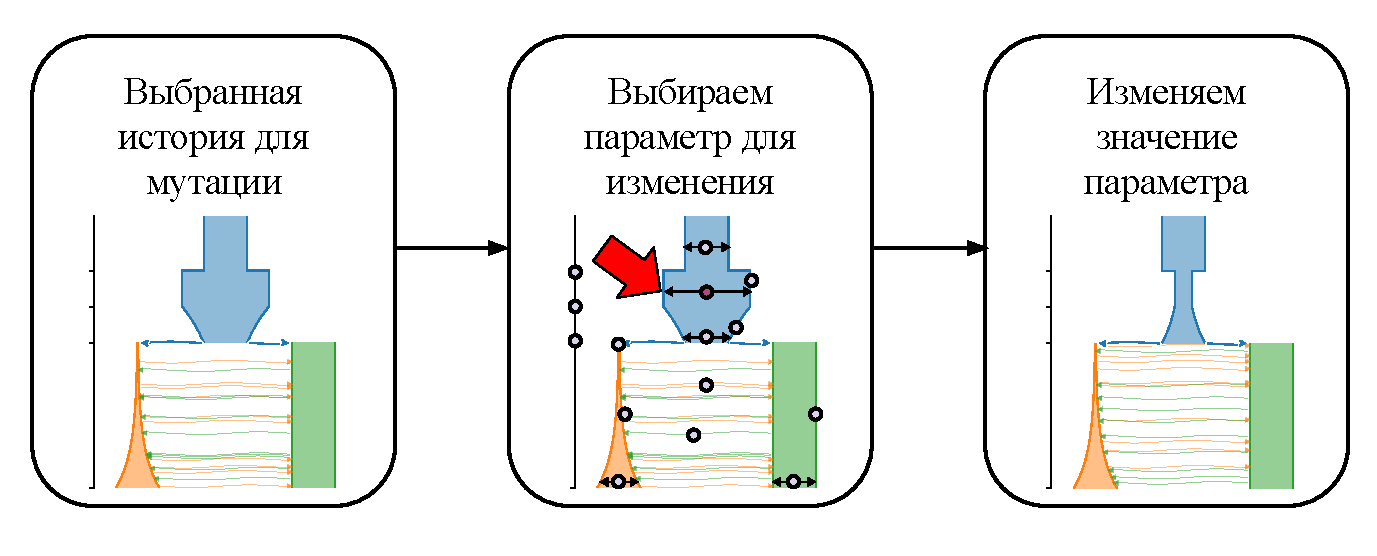
\includegraphics[width=\linewidth]{images/part2/genetics_algorithm/Mutation_rus.pdf}
  \caption{Пример применения оператора мутации разработанного генетического алгоритма}
  \label{fig:part2:mutation}
\end{figure}

\begin{algorithm}
\caption{Псевдокод оператора мутации разработанного генетического алгоритма. На вход подается целевая функция $f$, особь $x$ с геномом $x.\text{params}$ в виде вектора значений параметров длины $n$, сила мутации $\mu_\text{s}$ и степень мутации $\mu_\text{r}$}
\label{alg:part2:mutation}
\begin{algorithmic}[1]
\Function{Mutate}{$f, x, \mu_s, \mu_r$}
\If{$x.\text{weights} == \text{None}$} 
    \State {$x.\text{weights} \leftarrow \{1\}^n$} \Comment{Задаем веса, если они не были заданы раньше}
\EndIf
\State $k \leftarrow$ \Call{BinomialRandom}{$\mu_{\text{s}}, n$} \Comment{Число параметров для изменения}
\State $\omega \leftarrow \left\{\frac{x.\text{weights}[i]}{\sum_{j=1}^n x.\text{weights}[j]}\right\}_{i=1}^n$  \Comment{Вероятность изменения параметра прямо пропорциональна его весу}
\State $\text{inds} \leftarrow$ \Call{DiscreteRandom}{$\{i\}_{i=1}^n, p=\omega, \text{size}=k$} \Comment{Индексы параметров}
\State {$x_{\text{mut}} \leftarrow x$}
\For {$i \in \text{inds}$} \Comment{Изменяем каждый параметр}
    \State $s  \leftarrow$ \Call{UniformRandom}{$\{-1, +1\}$}
    \State $\sigma  \leftarrow$ \Call{SigmaBasedOnThreeSigmaRule}{$\mu_\text{r}, 0.0, 1.0$}
    \State $\lambda  \leftarrow$ \Call{TruncNormRandom}{$\mu_\text{r}, \sigma, 0.0, 1.0$}
    \State $x_{\text{mut}}.\text{params}[i] \leftarrow (1 + s \cdot \lambda) \cdot x_{\text{mut}}.\text{params}[i]$
\EndFor
\If {$f(x_{\text{mut}}) < f(x)$} \Comment{Если произошло улучшение $f$}
    \For {$i \in \text{inds}$} \Comment{Обновляем веса}
        \State {$x_{\text{mut}}.\text{weights}[i] \leftarrow x_{\text{mut}}.\text{weights}[i] + 1$}
    \EndFor
\EndIf
\State $x_{\text{mut}}.\text{lastOperation} \leftarrow \text{\texttt{"Mutation"}}$
\State \Return $x_{\text{mut}}$
\EndFunction
\end{algorithmic}
\end{algorithm}

\FloatBarrier
%\subsection{Адаптивные сила и степень мутации}

На начальных итерациях генетического алгоритма сильные мутации большого числа генов гораздо эффективнее слабых мутаций небольшого числа генов, тогда как при приближении к оптимальному решению все наоборот.
Поэтому были разработаны \textbf{адаптивные степень и сила мутации}, которые могут изменяться в процессе работы алгоритма.
Есть несколько способов сделать параметр алгоритма адаптивным, одним из самых популярных является алгоритм одной пятой~\cite{schumer1968adaptive}.
Рассмотрим его применение к степени мутации $\mu_\text{r}$: на каждой итерации, если у нас произошло событие «успеха» --- улучшение целевой функции, то умножаем степень мутации $\mu_\text{r}$ на константу $C_{\mu_\text{r}}\in[1,2]$.
Если лучшее решение осталось прежним, то значение $\mu_\text{r}$ делится на корень четвертой степени из $C_{\mu_\text{r}}$, уменьшая меру изменения генов при применении мутации.
В случае силы мутации $\mu_\text{s}$ был предложен аналогичный подход, отличающийся тем, что для «успеха» дополнительно требуется проверить условие того, что новое лучшее решение было получено с помощью мутации.

Таким образом, частые обновления текущей наилучшей особи с помощью оператора мутации приводят к увеличению числа изменяющихся генов, а также к увеличению меры их изменения.
При приближении к оптимальному решению и сходимости алгоритма происходит уменьшение частоты обновлений, числа генов и меры их изменения уменьшаются, что приводит к более точному поиску.
Псевдокод обновления адаптивных силы и степени мутации по алгоритму «одной пятой» представлен в листинге~\ref{alg:part2:adaptive_change}.

\begin{algorithm}
\caption{Процедура обновления силы и степени мутации по алгоритму «одной пятой». На вход алгоритм принимает значение $\mu$, которое может быть $\mu_\text{s}$ или $\mu_\text{r}$, и соответствующую ему константу $C_\mu$ --- $C_{\mu_\text{s}}$ и $C_{\mu_\text{r}}$ соответственно}
\label{alg:part2:adaptive_change}
\begin{algorithmic}[1]
\Function{UpdateValue}{$success, \mu, C_{\mu}$}
\If {$success == True$} \Comment{Правило «одной пятой»}
    \State $\mu \leftarrow c \cdot \mu$
\Else
    \State $\mu \leftarrow \frac{1}{c^{0.25}} \cdot \mu$
\EndIf
\Return $\mu$
\EndFunction
\end{algorithmic}
\end{algorithm}

\FloatBarrier
%\subsection{Кроссовер двух демографических историй}

Следующим оператором разработанного генетического алгоритма является \textbf{оператор скрещивания}.
При его применении выбираются две особи из текущего поколения, которые называются \textit{родителями}, и на основе их геномов строится геном их \textit{потомка}.
В разработанном методе родители выбираются случайным образом по тому же правилу, что и особи для применения оператора мутации --- вероятность выбора прямо пропорциональна значению функции приспособленности.
Каждый ген в геноме потомка выбирается случайным образом с равной вероятностью от одного или второго родителя --- был применен равномерный вид скрещивания.
На рисунке~\ref{fig:part2:crossover} показано применение операции скрещивания для выбранных родителей.
Псевдокод процедуры кроссовера представлен в листинге~\ref{alg:part2:crossover}.

\begin{figure}[ht]
  \centering
   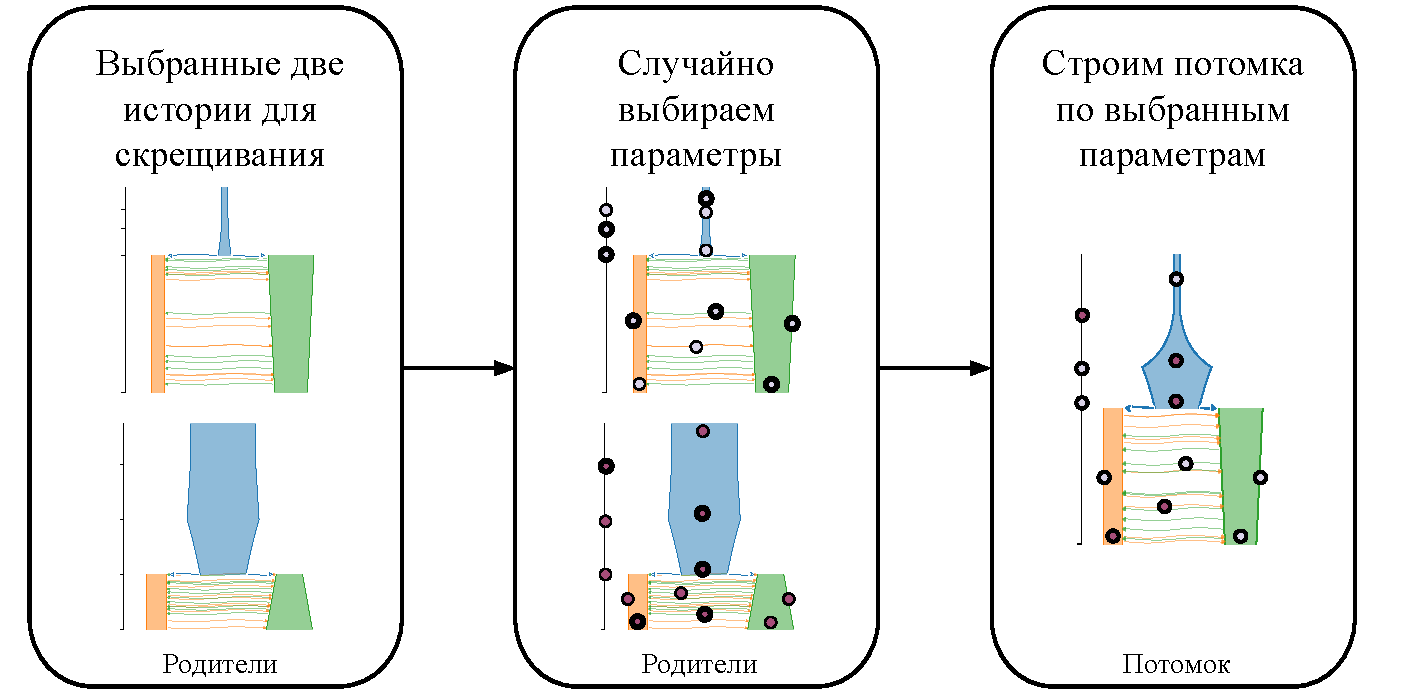
\includegraphics[width=\linewidth]{images/part2/genetics_algorithm/Cross_rus.pdf}
  \caption{Пример применения оператора кроссовера разработанного генетического алгоритма}
  \label{fig:part2:crossover}
\end{figure}

\begin{algorithm}
\caption{Псевдокод оператора скрещивания разработанного генетического алгоритма. На вход подаются две выбранные особи-родителя $x_1$ и $x_2$, геном каждой из которых представлен в виде вектора значений параметров длины $n$}
\label{alg:part2:crossover}
\begin{algorithmic}[1]
\Function{CrossOver}{$x_1, x_2$}
\State $x \leftarrow $ \Call{CreateNewSolution}{\ }
\State $x.\text{params} \leftarrow [\ ]$ 
\For {$i \leftarrow 1..n$} \Comment{Берем нужные параметры от родителей}
    \State $p \leftarrow$ \Call{UniformRandom}{$\{1, 2\}$}
    \If {$p == 1$}
        \State $x.\text{params}$.Add($x_1.\text{params}[i]$)
    \Else \Comment{Если $p == 2$}
        \State $x.\text{params}$.Add($x_2.\text{params}[i]$)
    \EndIf
\EndFor
\State $x.\text{lastOperation} \leftarrow$ \texttt{"CrossOver"}
\State \Return $x$
\EndFunction
\end{algorithmic}
\end{algorithm}

\FloatBarrier
\textbf{Правило трех сигм и алгоритм выбора дисперсии усеченного нормального распределения.}
%\label{sec:part2:genetic_algorithm:3_sigma_rule}
При применении оператора мутации для изменения генома особи используется усеченное нормальное распределение $\hat{N}(\mu, \sigma^2, a, b)$.
Оно определяется четырьмя параметрами: математическим ожиданием $\mu$, дисперсией $\sigma^2$, границами области значений $[a, b]$.
Математическое ожидание этого распределения равно параметру силы мутации $\mu_\text{r}$, а выбор дисперсии $\sigma^2$ выполняется согласно специально разработанной процедуре.
Опишем разработанную процедуру выбора среднеквадратичного отклонения $\sigma$, а, следовательно, и дисперсии $\sigma^2$, при заданном математическом ожидании $\mu$.
Идея основана на \textit{правиле трех сигм}~\cite{pukelsheim1994three}.

В соответствии с этим правилом вероятность того, что абсолютное отклонение нормальной случайной величины от математического ожидания будет меньше трех среднеквадратичных отклонений, равна $\sim{0{,}997}$:
$$P(|\xi - \mu| < 3\sigma) 	\approx 0{,}997,\quad \xi \sim N(\mu, \sigma^2).$$

Данное правило можно переформулировать следующим образом: при сэмплировании случайной величины из распределения $N(\mu, \sigma^2)$ с вероятностью $99{,}7$\% значение будет лежать в интервале $[\mu - 3\sigma, \mu + 3 \sigma]$.
Рисунок~\ref{fig:part2:3sigma_rule} иллюстрирует правило трех сигм.
На рисунке представлен график плотности нормального распределения $N(0, 1)$, на котором наглядно продемонстрированы несколько интервалов области значений и вероятности того, что выборка случайной величины будет принадлежать этим интервалам.
Синие области соответствуют интервалам, которые имеют ширину, равную среднеквадратичному отклонению $\sigma$.
%Проценты, указанные для каждой области, соответствуют доле значений лежащих в пределах области по оси абсцисс.
Правило трех сигм утверждает, что около $99{.}7$\% значений случайной величины лежат в пределе трех среднеквадратичных отклонений $\sigma$ от математического ожидания $\mu$.

\begin{figure}[ht]
    \centering
    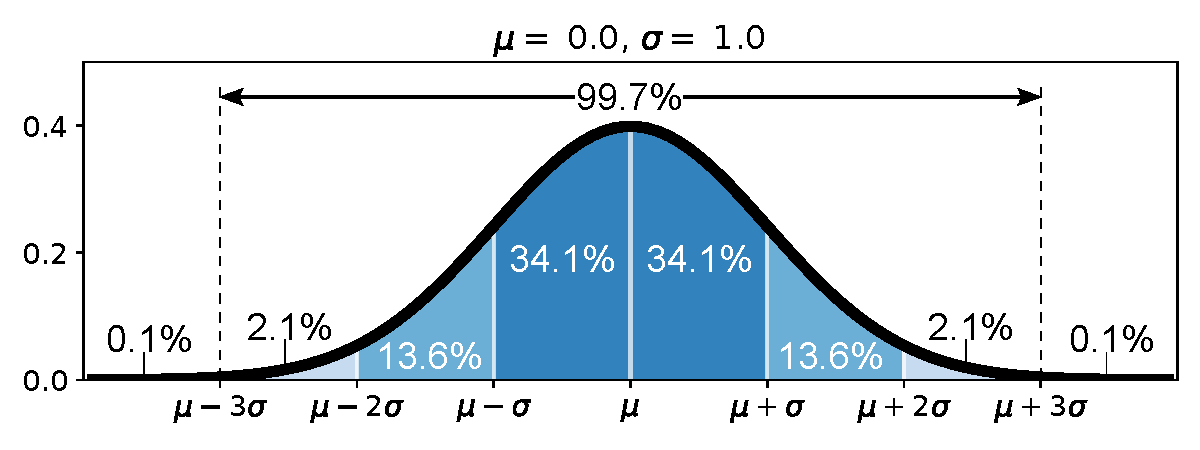
\includegraphics[width=0.8\linewidth]{images/part2/genetics_algorithm/3sigma_rule_fixed.pdf}
    \caption{Плотность нормального распределения $N(\mu, \sigma^2)$ и иллюстрация правила трех сигм}
    \label{fig:part2:3sigma_rule}
\end{figure}

На основе правила трех сигм был разработан метод выбора среднеквадратичного отклонения $\sigma$ по заданным значениям среднего $\mu$, нижней и верхней границ допустимых значений случайной величины.
Пусть требуется построить распределение случайной величины, которое имеет математическое ожидание $\mu$ и область определения, равную отрезку $[a, b]$.
Рассмотрим нормальное распределение $\hat{N}(\mu, \sigma^2, a, b)$, усеченное на отрезок $[a, b]$.
Оно определяется плотностью нормального распределения $N(\mu, \sigma^2)$, значения которой равны нулю за пределами указанного интервала, и которая умножена на константу таким образом, чтобы ее интеграл был равен единице.
Выберем среднеквадратичное отклонение $\sigma$, как треть расстояния от среднего $\mu$ до границ отрезка $[a, b]$.
Тогда согласно правилу трех сигм значения случайной величины будут лежать на отрезке с вероятностью 99.7\%.
В случае если отрезок не симметричен относительно среднего $\mu$, среднеквадратичное отклонение выбирается как треть наибольшего расстояния от среднего до границ отрезка.

Псевдокод процедуры $\text{SigmaBasedOnThreeSigmaRule}$ выбора среднеквадратичного отклонения для усеченного нормального распределения на отрезке $[a, b]$ при известном математическом ожидании $\mu \in [a, b]$ представлен в листинге~\ref{alg:part2:3sigma_alg}.
Примеры плотностей усеченного нормального распределения на отрезке $[0, 1]$, построенных для разных значений среднего $\mu_r$ и среднеквадратичного отклонения $\sigma$, выбранного с помощью разработанного метода, основанного на правиле трех сигм, приведены на рисунке~\ref{fig:part2:3sigma_example}.

\begin{algorithm}
\caption{Процедура выбора среднеквадратичного отклонения для усеченного нормального распределения на отрезке $[a, b]$ при известном математическом ожидании $\mu \in [a, b]$ по правилу трех сигм}
\label{alg:part2:3sigma_alg}
\begin{algorithmic}[1]
\Function{SigmaBasedOnThreeSigmaRule}{$\mu, a, b$}
    \State {$\sigma \leftarrow \frac{\max\{(\mu - a), (b - \mu)\}}{3}$}
\State \Return $\sigma$
\EndFunction
\end{algorithmic}
\end{algorithm}

\begin{figure}[ht]
    \centering
    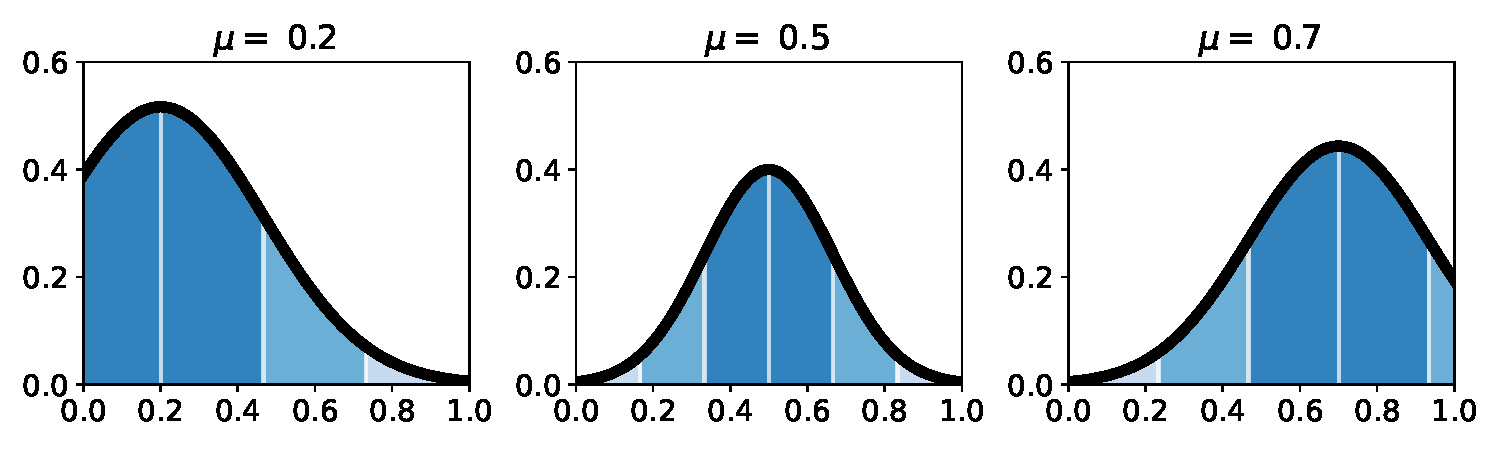
\includegraphics[width=\linewidth]{images/part2/genetics_algorithm/3sigma_examples.pdf}
    \caption{Примеры плотности усеченного нормального распределения~$\hat{N}(\mu, \sigma^2, 0, 1)$ на отрезке $[0,1]$, у которого среднеквадратичное отклонение $\sigma$ выбрано в соответствии с разработанным методом}
    \label{fig:part2:3sigma_example}
\end{figure}


\FloatBarrier
\subsection{Реализация разработанного метода, основанного на комбинации генетического алгоритма и локального поиска}
\label{sec:part2:genetic_algorithm:implementation}

Для реализации разработанного метода, основанного на комбинации генетического алгоритма и локального поиска, был реализован модуль \texttt{optimizers} на языке программирования Python.
Этот модуль содержит различные методы оптимизации, которые применимы для решения задачи оптимизации произвольной функции $f$.
Задача настройки параметров моделей демографической истории рассматривается, как задача оптимизации функции $f_\mathcal{M}(\theta) = \log(\mathcal{L}(\theta | \mathfrak{D}))$, которую можно решать с использованием методов рассматриваемого модуля.
Структура классов реализованного модуля \texttt{optimizers} представлена на рисунке~\ref{fig:part2:optimizers_classes}.

\begin{figure}[ht]
    \centering
    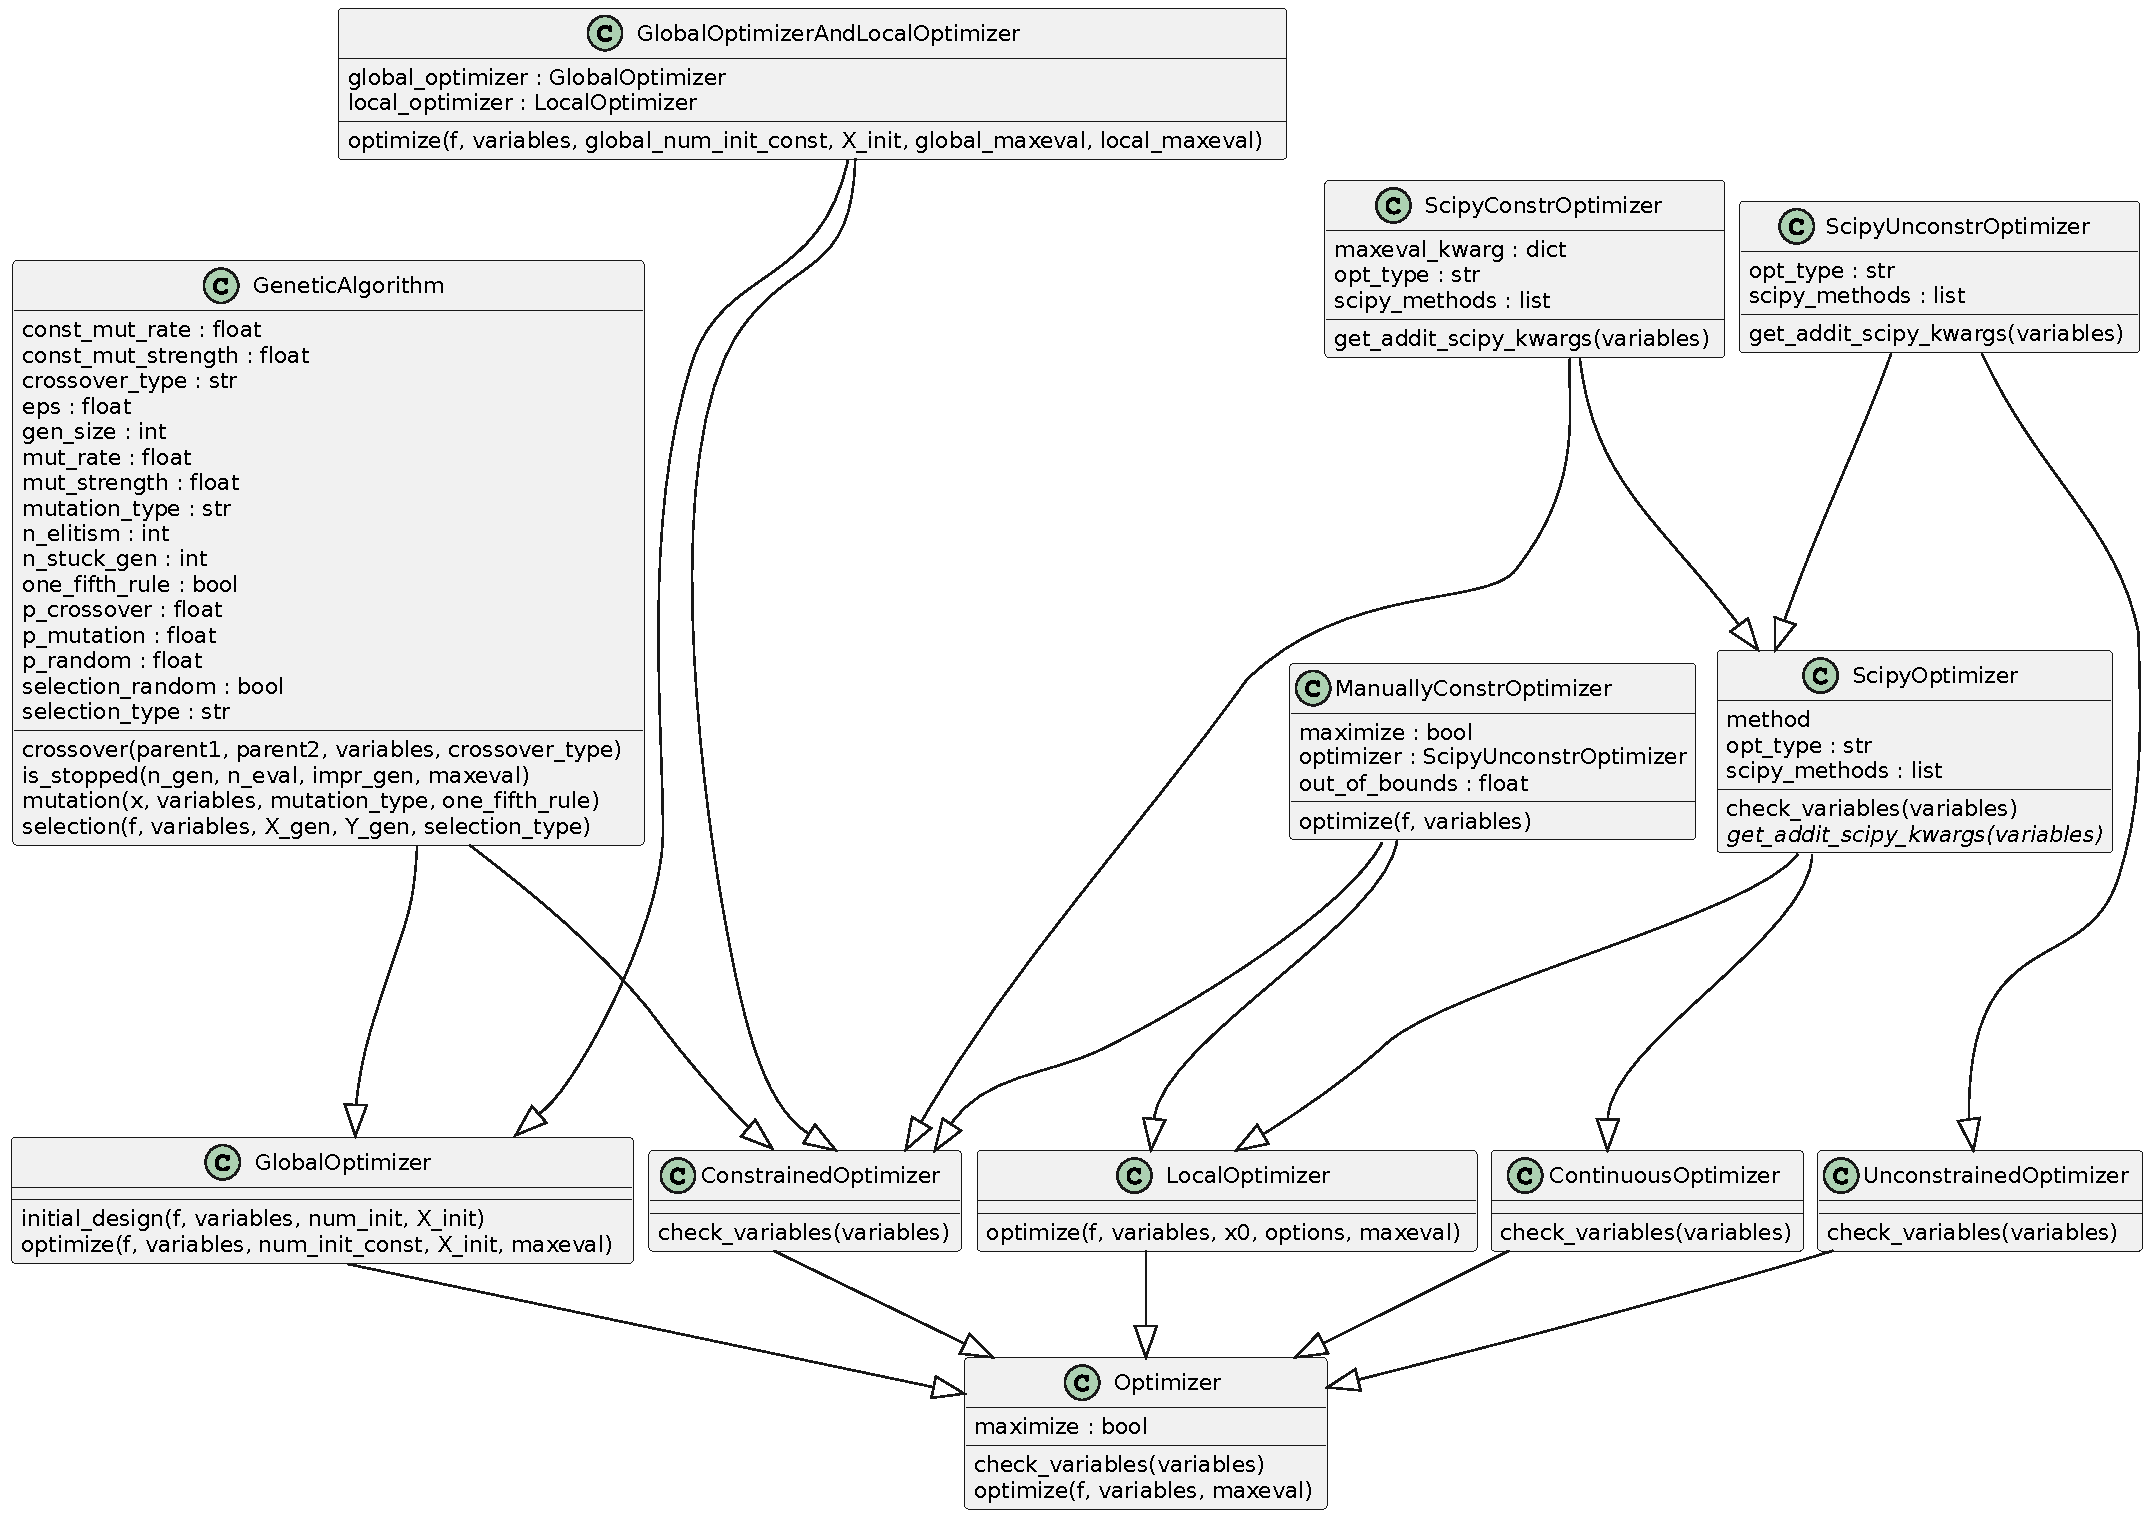
\includegraphics[width=\linewidth]{images/part5/optimizer_classes_short_wo_bo.pdf}
    \caption{Структура классов разработанного модуля \texttt{optimizers}}
    \label{fig:part2:optimizers_classes}
\end{figure}

Основной абстрактный класс \texttt{Optimizer} соответствует произвольному методу оптимизации.
У объекта этого класса задан атрибут \texttt{maximize}, который определяет какая задача решается: минимизации или максимизации целевой функции.
Абстрактная процедура \texttt{optimize} запускает процесс поиска оптимальных значений параметров \texttt{variables} целевой функции \texttt{f}, который может быть ограничен \texttt{maxeval} --- максимальным числом вычислений.
От этого абстрактного класса наследуются:
\begin{itemize}
    \item абстрактный класс \texttt{ContinuousOptimizer} методов решения задач оптимизации непрерывных параметров;
    \item абстрактный класс \texttt{UnconstrainedOptimizer} методов решения задач безусловной оптимизации --- без ограничений на область значений параметров;
    \item абстрактный класс \texttt{ConstrainedOptimizer} методов решения задач условной оптимизации --- с ограничениями на область значений параметров;
    \item абстрактный класс \texttt{GlobalOptimizer} методов глобальной оптимизации;
    \item абстрактный класс \texttt{LocalOptimizer} методов локальной оптимизации.
\end{itemize}

Рассмотрим реализацию методов локальной оптимизации.
Для этого была использована библиотека SciPy~\cite{virtanen2020scipy}, которая предоставляет множество методов, используемых в существующих программных решениях вывода демографической истории.
Для сохранения предложенного интерфейса с процедурой \texttt{optimize} были реализованы классы-обертки \texttt{ScipyOptimizer}, \texttt{ScipyConstrOptimizer} и \texttt{ScipyUnconstrOptimizer}, которые соответствуют абстрактному классу произвольного метода, классу методов безусловной и условной оптимизации, представленных в библиотеке SciPy, соответственно.
Дополнительный класс \texttt{ManuallyConstrOptimizer} позволяет использовать методы безусловной оптимизации из библиотеки SciPy для решения задач условной оптимизации.
Например, метод BFGS, который является методом безусловной оптимизации,  был реализован, как объект класса \texttt{ManuallyConstrOptimizer} для применения его для решения условной задачи вывода демографической истории.
Были реализованы следующие методы, доступные в библиотеке SciPy:
\begin{itemize}
    \item метод BFGS --- объект класса \texttt{ManuallyConstrOptimizer};
    \item метод L-BFGS-B --- объект класса \texttt{ScipyConstrOptimizer};
    \item метод Пауэлла --- объект класса \texttt{ManuallyConstrOptimizer};
    \item метод Нелдера-Мида --- объект класса \texttt{ManuallyConstrOptimizer}.
\end{itemize}

Реализация методов глобальной оптимизации включает два метода: генетический алгоритм (класс \texttt{GeneticAlgorithm}) и разработанный комбинированный метод (класс \texttt{GlobalOptimizerAndLocalOptimizer}).
Генетический алгоритм был реализован без использования сторонних библиотек.
Он имеет процедуру \texttt{crossover} операции скрещивания, процедуру \texttt{mutation} операции мутации и процедуру \texttt{selection} отбора --- вычисление целевой функции на множестве особей и выбор наиболее приспособленных.
Дополнительная процедура \texttt{is\_stopped} соответствует критерию останова.

\textbf{Разработанный комбинированный метод} реализован, как объект класса \texttt{GlobalOptimizerAndLocalOptimizer}.
Этот класс позволяет комбинировать любой реализованный метод глобальной оптимизации с методом локальной оптимизации для последовательного запуска.
Реализация разработанного метода на основе комбинации генетического алгоритма и метода BFGS локальной оптимизации с помощью модуля \texttt{optimizers} показана на рисунке~\ref{fig:part2:optimizer_implementation}.

\begin{figure}[ht]
    \centering
    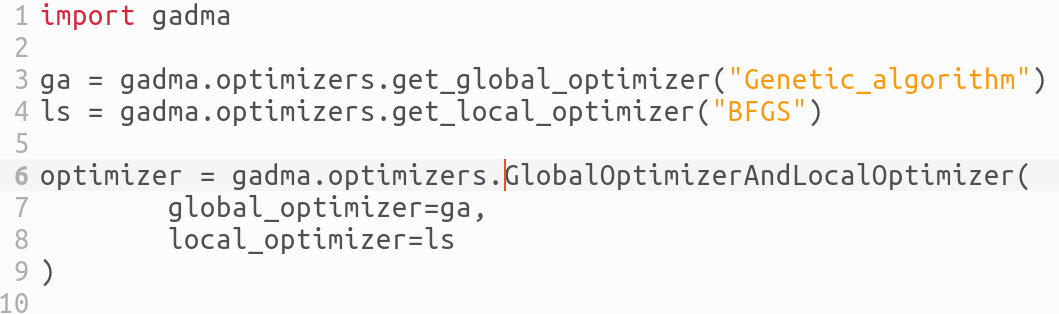
\includegraphics[width=\linewidth]{images/part2/genetics_algorithm/optimizer_implementation.png}
    \caption{Реализация разработанного комбинированного метода с помощью модуля \texttt{optimizers}}
    \label{fig:part2:optimizer_implementation}
\end{figure}

Модуль \texttt{optimizers} можно использовать для решения произвольной задачи оптимизации.
Пример решения задачи поиска минимума функции Розенброка~\cite{rosenbrock1960automatic} (рисунок~\ref{fig:part1:opt:rosenbrock}) представлен на рисунке~\ref{fig:part2:ga_implementation:rosenbrock_ex}.
Заметим, что программный код использует модуль \texttt{variables}, который был предложен для реализации моделей демографической истории и описан в разделе~\ref{sec:part2:new_models}.
Вывод, полученный путем запуска программного кода поиска минимума функции Розенброка, представлен на рисунке~\ref{fig:part2:ga_implementation:rosenbrock_out}.

\begin{figure}[ht]
    \centering
    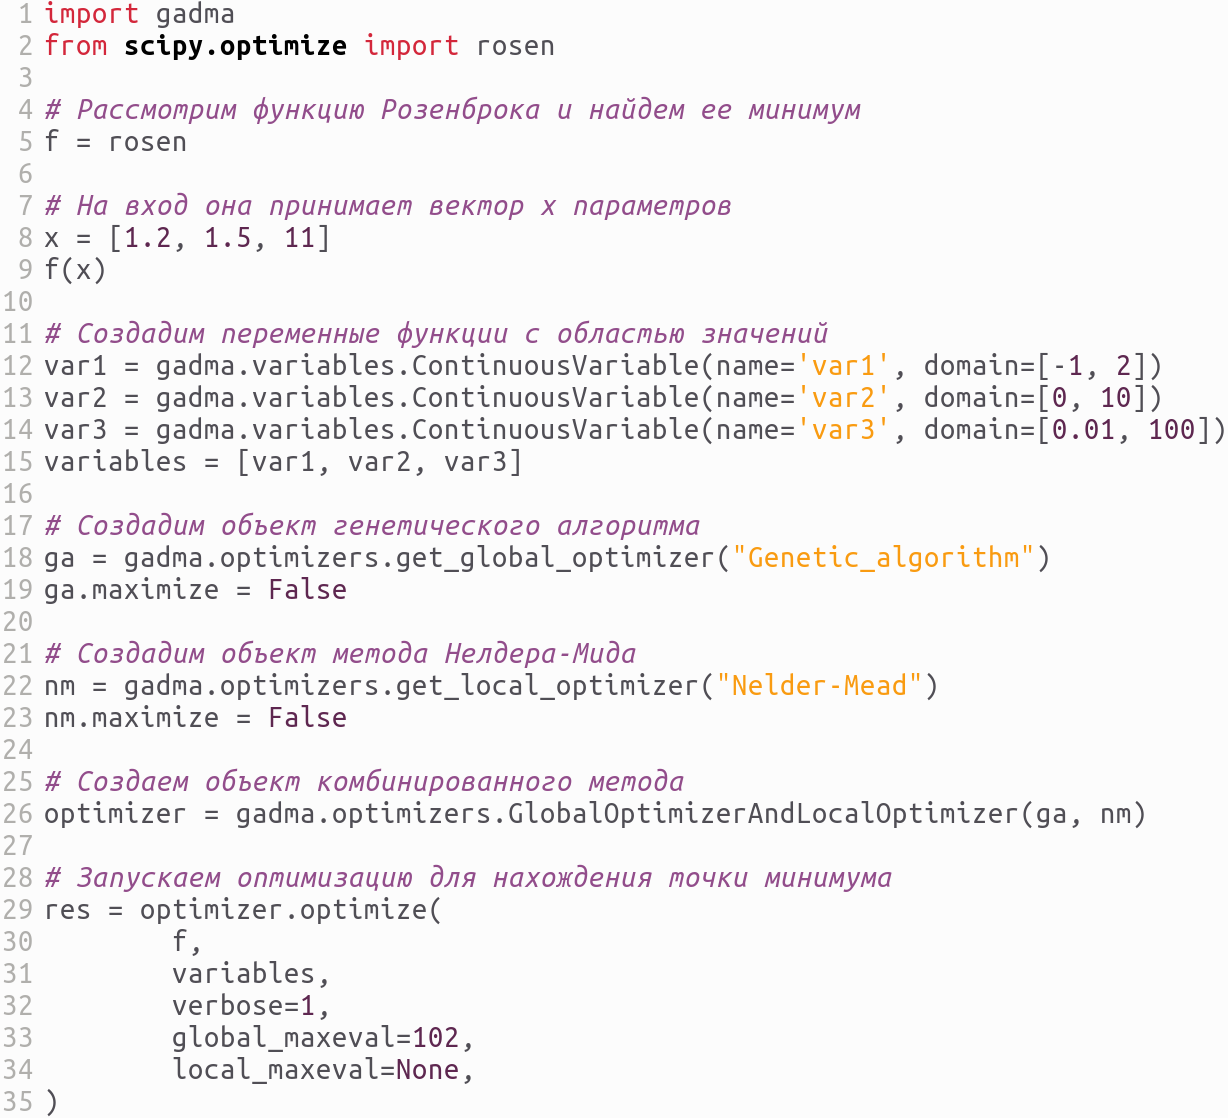
\includegraphics[width=\linewidth]{images/part2/genetics_algorithm/example_run.png}
    \caption{Применение разработанного комбинированного метода на основе генетического алгоритма, реализованного с помощью модуля \texttt{optimizers}, для поиска точки минимума функции Розенброка}
    \label{fig:part2:ga_implementation:rosenbrock_ex}
\end{figure}

\begin{figure}[ht]
    \centering
    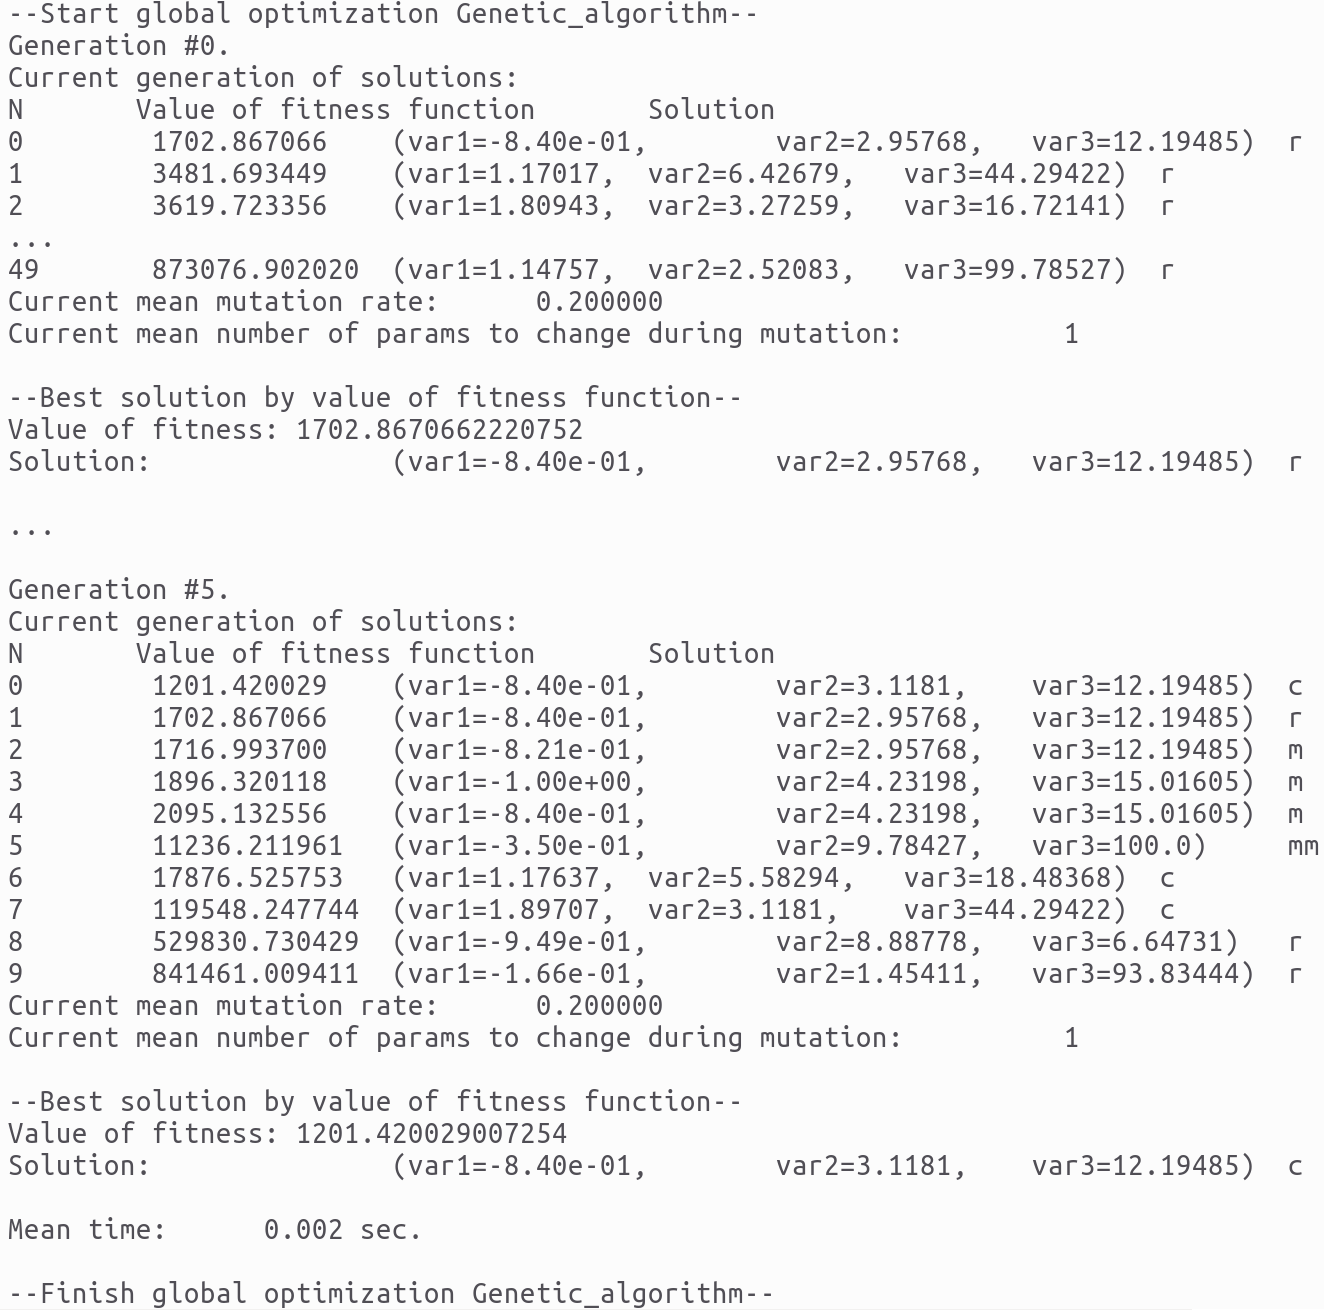
\includegraphics[width=\linewidth]{images/part2/genetics_algorithm/ga_output.png}
    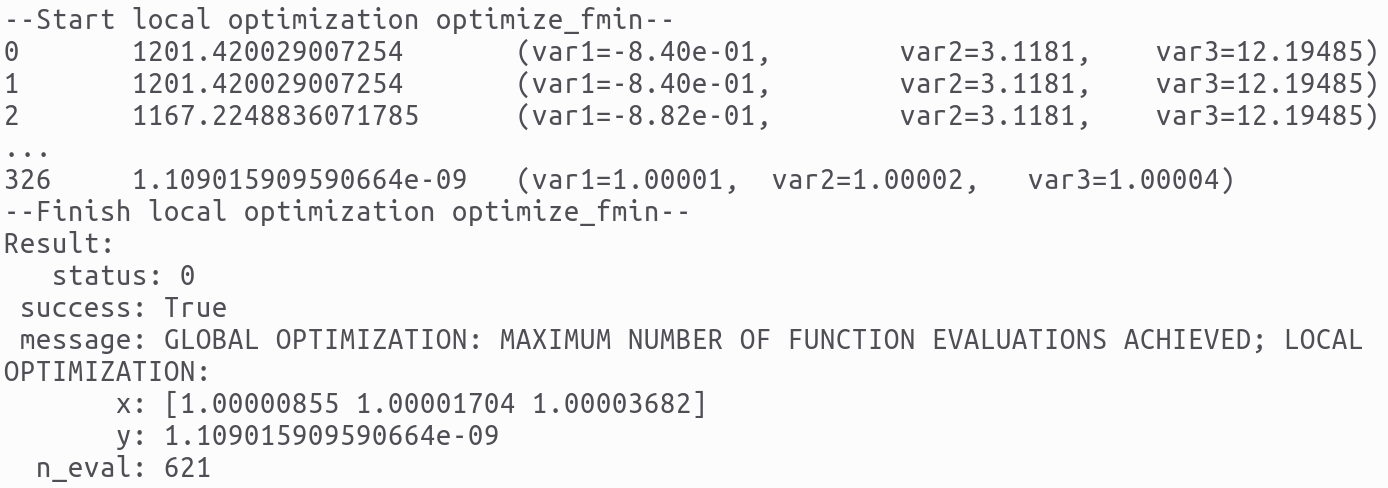
\includegraphics[width=\linewidth]{images/part2/genetics_algorithm/ls_output.png}
    \caption{Пример вывода программы, представленной на рисунке~\ref{fig:part2:ga_implementation:rosenbrock_ex}}
    \label{fig:part2:ga_implementation:rosenbrock_out}
\end{figure}

\FloatBarrier
\subsection{Настройка гиперпараметров разработанного генетического алгоритма}
\label{sec:part2:genetic_algorithm:hpo}

\textit{Гиперпараметр} --- это параметр алгоритма.
Производительность любого алгоритма зависит от значений его гиперпараметров --- от его \emph{конфигурации}.
Одним из классических примеров является темп (learning rate) обучения нейронной сети.
Проблема нахождения гиперпараметров, обеспечивающих наилучшую сходимость алгоритма на нескольких экземплярах задачи, называется \textit{задачей конфигурации алгоритма}.
Экземплярами задачи могут быть различные постановки этой задачи для разных данных.
\emph{Задачу конфигурации алгоритма} можно сформулировать следующим образом: для  алгоритма $A$, набора экземпляров задачи $I$ и \textit{функции стоимости}  $c$ найти набор гиперпараметров для $A$, который является наилучшим относительно $c$ на всем множестве $I$.
Обычно функция стоимости $c$ основана либо на времени, необходимом для решения проблемы, либо на оценке качества решения, достигнутом в рамках фиксированного бюджета.
SMAC~\cite{hutter2011sequential, lindauer2021smac3} --- это программное обеспечение, реализующее метод, основанный на байесовской оптимизации, для решения задачи конфигурации алгоритма.

Метод байесовской оптимизации основан на использовании \textit{суррогатной модели} для аппроксимации целевой функции $f$ и \textit{функции выбора} $\alpha$ для поиска многообещающих точек на каждой итерации.
На каждой итерации происходит аппроксимация суррогатной моделью по имеющемуся набору точек $\theta_1, y_1, \theta_2, y_2, \dots, \theta_n, y_n$, где $y_i = f(\theta_i)$.
Затем по аппроксимации строится функция выбора $\alpha$ и происходит поиск точки ее максимума, которая затем выбирается как новая точка для вычисления целевой функции.
Подробное описание метода байесовской оптимизации приведено в разделе~\ref{sec:part2:bayesian_optimization}.

В качестве суррогатной модели байесовская оптимизация в SMAC использует случайный лес, а в качестве функции выбора функцию ожидаемого улучшения (Expected Improvement, EI):
$$\alpha_{\mathrm{EI}}(\theta) = \mathbb{E}_\theta \bigl[\max(0, \hat{f}(\theta)) - \max_{1 \leq i \leq n}(y_i)\bigr],$$
где $\hat{f}$ --- построенная аппроксимация целевой функции $f$.
В отличие от классической байесовской оптимизации, SMAC реализует многокритериальную оптимизацию, так как рассматривает несколько экземпляров задачи.
Таким образом, цель состоит в поиске решения, которое будет наилучшим для всех экземпляров задачи в соответствии с заданной функцией стоимости $c$.
Данная многокритериальность может быть решена различными способами.
SMAC сводит эту задачу к задаче обычной однокритериальной оптимизации, используя в качестве целевой функции среднее значение функций стоимости на экземплярах задач.
Еще одним расширением метода является «интенсификация» --- процедура сравнения конфигураций гиперпараметров и выбора наилучшей.
Метод «интенсификации», реализованный в SMAC, рассматривает конфигурацию как новую лучшую, если она лучше, чем текущая лучшая на наборе пар из экземпляров задачи и генераторов случайных чисел (random seed).
Учитывание генераторов случайных чисел позволяет проводить честные сравнения двух конфигураций на одном экземпляре задачи в случае, если рассматриваемый алгоритм не детерминированный.
Используемый набор пар расширяется каждый раз, когда тестируемая конфигурация оказывается хуже текущей лучшей, с которой и происходит сравнение. 
Таким образом, этот набор всегда растет и требуется все больше и больше сравнений, чтобы превзойти текущую лучшую конфигурацию.

Из изложенного следует, что SMAC --- это итеративный метод, который на каждой итерации поддерживает наилучшую конфигурацию гиперпараметров оптимизируемого алгоритма.
Новая многообещающая конфигурация выбирается и сравнивается с текущей лучшей в рамках процедуры «интенсификации» на каждой итерации.
В результате в качестве ответа SMAC предоставляет конфигурацию гиперпараметров для алгоритма, которая имеет наилучшее по среднему значение функции стоимости.
SMAC был использован для поиска оптимальных значений гиперпараметров разработанного генетического алгоритма для поиска демографической истории популяций.

Метод оптимизации, такой как генетический алгоритм, имеет несколько гиперпараметров, и их число изменяется в зависимости от конкретной реализации.
Генетический алгоритм, представленный в разделе~\ref{sec:part2:genenic_algorithm}, имеет десять гиперпараметров. 
Каждая особь в поколении представляется в виде массива значений параметров $\theta$ модели $\mathcal{M}$ демографической истории.
Начальное множество решений, называемое поколением, формируется процедурой \textit{начального дизайна}, которая генерирует множество случайных параметров.
Размер этого набора определяется значением гиперпараметра \texttt{n\_init\_const}: число решений в начальном поколении равно числу параметров модели, умноженному на \texttt{n\_init\_const}. 
Размер каждого поколения в генетическом алгоритме равен значению гиперпараметра \texttt{gen\_size}.
Новое поколение строится итеративно с помощью мутации, скрещивания и отбора лучших по значению вероятностных моделей.
Доли наиболее адаптированных, мутировавших, скрещенных и случайных моделей, формирующих новое поколение, определяются \texttt{p\_elitism}, \texttt{p\_mutation}, \texttt{p\_crossover}, \texttt{p\_random } гиперпараметрами соответственно.
Особым случаем является процесс адаптивной мутации: дополнительно содержащий параметры \texttt{mutation\_strength} и \texttt{mutation\_rate}, которые определяют, сколько параметров модели и насколько сильно будут изменяться их значения
Каждый из этих двух гиперпараметров изменяется в процессе работы генетического алгоритма по правилу одной пятой: чем ближе к оптимуму, тем меньше изменений в процессе мутации.
Константы правила одной пятой (\texttt{const\_mutation\_strength}, \texttt{const\_mutation\_rate}) также являются гиперпараметрами генетического алгоритма.
Всего было выделено десять гиперпараметров генетического алгоритма: два имеют целочисленные дискретные значения, а восемь --- численные непрерывные.
Краткое описание каждого гиперпараметра представлено в таблице~\ref{tab:hyper_descr}.

\begin{table}[ht]
    \caption{Краткое описание и обозначения гиперпараметров разработанного генетического алгоритма.}
    \centering
    \resizebox{\linewidth}{!}{%
    \begin{tabular}{|p{4.8cm}|p{1.9cm}|p{5.5cm}|}
        \hline
        \multirow{2}{*}{ID гиперпараметра}  & Обозначение & \multirow{2}{*}{Описание гиперпараметра} \\
         & в псевдокоде & \\
        \hline
        \texttt{gen\_size} & $N_{GEN}$ & Число решений в одном поколении генетического алгоритма \\
        \hline
        \texttt{n\_init\_const} & --- & Константа, определяющая число случайных решений в
        случайно сгенерированном поколении \\
        \hline
        \texttt{p\_elitism} & $N_\text{B} / N_{\text{gen}}$ & Доля лучших решений, перенесенных в новое поколение \\
        \hline
        \texttt{p\_mutation} & $N_\text{M} / N_{\text{gen}}$ & Доля мутировавших решений в новом поколении \\
        \hline
        \texttt{p\_crossover} & $N_\text{C} / N_{\text{gen}}$ & Доля решений, образованных кросинговером, в новом поколении \\
        \hline
        \texttt{p\_random} & $N_\text{R} / N_{\text{gen}}$ & Доля случайно сгенерированных решений в новом поколении \\
        \hline
        \texttt{mutation\_strength} & $\mu_\text{s}$ & Начальная сила мутации\\
        \hline
        \texttt{const\_mutation\_strength} & $C_{\mu_\text{s}}$ & Константа для изменения \texttt{mutation\_strength} во время генетического алгоритма согласно правилу одной пятой \\
        \hline
        \texttt{mutation\_rate} & $\mu_\text{r}$ & Начальная степень мутации \\
        \hline
        \texttt{const\_mutation\_rate} & $C_{\mu_\text{r}}$ & Константа для изменения \texttt{mutation\_rate} во время генетического алгоритма согласно правилу одной пятой \\
        \hline
    \end{tabular}%
    }
    \label{tab:hyper_descr}
\end{table}

\begin{table}[ht]
    \caption{Начальные значения и область значений, используемые для оптимизации гиперпараметров разработанного генетического алгоритма. Первые два гиперпараметра \texttt{gen\_size} и \texttt{n\_init\_const} являются целыми числами и имеют дискретную область значений. Остальные восемь гиперпараметров являются непрерывными.}
    \centering
    \begin{tabular}{lcc}
        \toprule
        ID гиперпараметра & Начальное значение & Область значений \\
        \midrule
        \texttt{gen\_size} & 10 & $\{10, 50, 100\}$ \\
        \texttt{n\_init\_const} & 10 & $\{5, 10, 20\}$ \\
        \texttt{p\_elitism} & 0.2 & $[0, 1]$ \\
        \texttt{p\_mutation} & 0.3 & $[0, 1]$ \\
        \texttt{p\_crossover} & 0.3 & $[0, 1]$ \\
        \texttt{p\_random} & 0.2 & $[0, 1]$ \\
        \texttt{mutation\_strength} & 0.2 & $[0, 1]$ \\
        \texttt{const\_mutation\_strength} & 1.01 & $[1, 2]$ \\
        \texttt{mutation\_rate} & 0.2 & $[0, 1]$ \\
        \texttt{const\_mutation\_rate} & 1.02 & $[1, 2]$ \\
        \bottomrule
    \end{tabular}
    \label{tab:hyper_domain}
\end{table}

Начальные значения гиперпараметров в первой версии разработанного генетического алгоритма были настроены вручную в ходе вывода демографической истории двух популяций современных людей для модели и данных из \cite{gutenkunst2009inferring} (набор данных \texttt{2\_YRI\_CEU\_6\_Gut}).
Их значения представлены в таблице~\ref{tab:hyper_domain}.

\begin{figure}[ht]
    \centering
    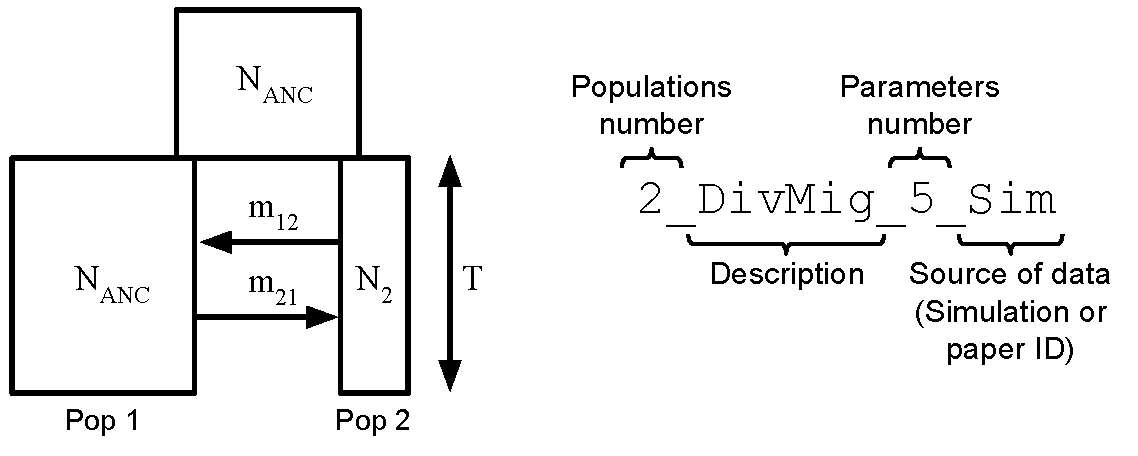
\includegraphics[width=0.6\linewidth]{images/part2/genetics_algorithm/deminf_data_example.pdf}
    \caption{Пример описание структурированного формата имени набора данных из пакета \texttt{deminf\_data v1.0.0}}
    \label{fig:part2:genetic_algorithm:HPO:datasets}
\end{figure}

Все используемые наборы данных были взяты из пакета Python \texttt{deminf\_data v1.0.0}, который доступен на платформе GitHub по ссылке: \url{https://github.com/noscode/demographic_inference_data}.
Каждый набор данных имеет структурированное имя (рисунок~\ref{fig:part2:genetic_algorithm:HPO:datasets}), которое представляет собой последовательность: а)~номер популяции, б) краткое описание демографической модели, в) число параметров и г) информация об источнике данных.

Метод SMAC был использован для настройки гиперпараметров разработанного генетического алгоритма.
Наборы данных были разделены на две группы: обучающие и тестовые.
Оптимизация выполнялась с использованием метода \moments для вычисления правдоподобия на четырех обучающих наборах данных, которые представляли экземпляры задачи.
Тестовые наборы данных были использованы для проверки производительности новых конфигураций после оптимизации с помощью SMAC.

Четыре набора данных были выбраны в качестве обучающих: три набора имели симулированные данные (\texttt{2\_BotDivMig\_8\_Sim}, \texttt{2\_DivMig\_5\_Sim}, \texttt{2\_ExpDivNoMig\_5\_Sim}) и один (\texttt{2\_YRI\_CEU\_6\_Gut}) содержал реальные генетические данные для современных человеческих популяций из работы~\cite{gutenkunst2009inferring}.
Обучающие набора данных имели одинаковое число популяций и размер генетических данных.

Тестовые набора данных являются более разнообразными: два набора данных (\texttt{1\_Bot\_4\_Sim}, \texttt{1\_AraTha\_4\_Hub}) для одной популяции с симулированными и реальными данными из \cite{huber2018gene},  два набора (\texttt{2\_ButAll\_3\_McC}, \texttt{2\_ButSynB2\_5\_McC}) для двух популяций бабочек из \cite{mccoy2014genomic}; один набор с симулированными генетическими данными для трех популяций (\texttt{3\_DivMig\_8\_Sim}); и один набор данных (\texttt{2\_YRI\_CEU\_struct\_11\_Nos}) с генетическими данными для двух популяций современного человека из \cite{gutenkunst2009inferring} и моделью расширенного класса.

Функция стоимости $c$ была определена как лучшее значение логарифма правдоподобия, достигнутое генетическим алгоритмом за фиксированное число вычислений.
Для остановки было использовано число вычислений, которое в 200 раз превышает число параметров модели в наборе данных.
Полный запуск генетического алгоритма может требовать как меньше, так и больше вычислений целевой функции в зависимости от набора данных, так как он имеет критерий остановки, основанный на сходимости оптимизации.

Во время первого запуска SMAC, все десять гиперпараметров (Таблица~\ref{tab:smac_results}) были оптимизированы. 
Затем два дискретных гиперпараметра (\texttt{gen\_size} и \texttt{n\_init\_const}) были зафиксированы в конфигурации, и запущены дополнительные пять попыток оптимизации гиперпараметров.
Во время второй попытки оптимизации с помощью SMAC значения дискретных гиперпараметров \texttt{gen\_size} и \texttt{n\_init\_const} были установлены на значения по умолчанию (10 и 10 соответственно).
Для третьей и четвертой попыток были протестированы альтернативные значения гиперпараметра \texttt{n\_init\_const} --- 5 и 20.
Затем размер поколения в генетическом алгоритме (\texttt{gen\_size}) был увеличен до 50, а гиперпараметр начального дизайна (\texttt{n\_init\_const}) был протестирован на значениях 10 и 20.
Значение \texttt{n\_init\_const} равное пяти было исключено, так как оно приводит к небольшому числу решений для первого поколения, которое имеет размер 50.

Было выполнено шесть попыток оптимизации гиперпараметров при помощи SMAC.
При первой попытке SMAC не смог найти конфигурацию гиперпараметров, превосходящую исходную.
В результате было получено пять новых конфигураций, которые были сравнены между собой для выбора наилучшей.
Полученные конфигурации представлены в таблице~\ref{tab:smac_results}.
Для оценки эффективности новых конфигураций и выбора наилучшей были проведены полные запуски генетического алгоритма.
Для каждой конфигурации и набора данных генетический алгоритм был запущен 128 раз с использованием двух методов вычисления правдоподобия: \moments и \momi.
Для остановки полных запусков генетического алгоритма использовался тот же или эквивалентный критерии, что и в исходной версии метода.
Например, генетический алгоритм с конфигурацией, где размер поколения (\texttt{gen\_size}) равен 10, был остановлен после 100 поколений без улучшения значения правдоподобия.
Для конфигураций с \texttt{gen\_size} равным 50 использовался эквивалентный критерий остановки --- отсутствие улучшений в течение 20 поколений.

\begin{table}[ht]
    \caption{Значения гиперпараметров генетического алгоритма после каждой попытки оптимизации с помощью SMAC}
    \centering
    \resizebox{\columnwidth}{!}{%
    \begin{tabular}{lcccccc}
    \toprule
    \multirow{2}{*}{ID Гиперпараметра} & \multicolumn{6}{c}{Номер попытки} \\
    & 1 (по умолчанию) & 2 & 3 & 4 & 5 & 6 \\
    \midrule
    \texttt{gen\_size} & 10 & 10$^\star$ & 10$^\star$ & 10$^\star$ & 50$^\star$ & 50$^\star$ \\
    \texttt{n\_init\_const} & 10 & 10$^\star$ & 5$^\star$ & 20$^\star$ & 10$^\star$ & 20$^\star$ \\
    \texttt{p\_elitism} & 0.20 & 0.30 & 0.30 & 0.40 & 0.40 & 0.40 \\
    \texttt{p\_mutation} & 0.30 & 0.20 & 0.20 & 0.10 & 0.08 & 0.10 \\
    \texttt{p\_crossover} & 0.30 & 0.30 & 0.30 & 0.30 & 0.42 & 0.46 \\
    \texttt{p\_random} & 0.20 & 0.20 & 0.20 & 0.20 & 0.10 & 0.04 \\
    \texttt{mutation\_strength} & 0.200 & 0.776 & 0.370 & 0.534 & 0.833 & 0.528 \\
    \texttt{const\_mutation\_strength} & 1.010 & 1.302 & 1.290 & 1.648 & 1.199 & 1.492 \\
    \texttt{mutation\_rate} & 0.200 & 0.273 & 0.886 & 0.882 & 0.595 & 0.345 \\
    \texttt{const\_mutation\_rate} & 1.020 & 1.475 & 1.942 & 1.417 & 1.645 & 1.472 \\
    \bottomrule
    \end{tabular}%
    }
    \begin{tablenotes}
      \footnotesize
      \item $^\star$Значения были зафиксированы во время оптимизации гиперпараметров с помощью SMAC.
    \end{tablenotes}
    \label{tab:smac_results}
\end{table}

Сравнение новых конфигураций было выполнено следующим образом.
Сначала были измерены темпы ускорения, которые представляют собой долю вычислений целевой функции, которая экономится при использовании новой конфигурации вместо исходной.
Например, если конфигурация по умолчанию в среднем выполняла $X$ вычислений целевой функции для набора данных, а новая конфигурация в среднем занимает $Y$ вычислений, то темп ускорения будет равен $\frac{X-Y}{X}$.
Затем, каждая новая конфигурация была сравнена с исходной с помощью сравнения финальных значений правдоподобия.
Для каждого набора данных новая конфигурация считается лучше, чем исходная, если медиана и оба квартиля из 128 значений правдоподобия выше, чем для конфигурации по умолчанию.
Если медиана и оба квартиля ниже, то производительность новой конфигурации на наборе данных считается хуже.
Во всех остальных случаях, конфигурации считаются несравнимыми.
Целью исследования является выбор такой конфигурации, которая работает быстрее и лучше, чем конфигурация по умолчанию на максимально возможном числе наборов данных, и работает хуже на минимальном числе наборов данных.

Темпы ускорения, вычисленные для новых конфигураций, представлены в таблице~\ref{tab:part2:genetic_algorithm:HPO:speedup}.
В среднем все новые конфигурации требуют меньшего числа вычислений, чем исходный генетический алгоритм.
Конфигурации, полученные в ходе попыток три, пять и шесть, являются самыми быстрыми.
Однако их финальные правдоподобия хуже, чем у конфигурации по умолчанию на большинстве наборов данных (рисунок~\ref{fig:part2:genetic_algorithm:HPO:ll_comp}).
Генетический алгоритм с конфигурациями, полученными в ходе попыток два и четыре, демонстрирует лучшую эффективность с точки зрения финального правдоподобия среди новых конфигураций.
Более того, генетический алгоритм с гиперпараметрами из попытки два имеет лучшие значения правдоподобия для \moments, в то время как конфигурация из попытки четыре имеет лучшие результаты для \momi.
Поскольку при оптимизации гиперпараметров использовался \moments движок, конфигурация номер два была выбрана как новые гиперпараметры для генетического алгоритма.
Рисунок~\ref{fig:part2:genetic_algorithm:HPO:final_comp} суммирует улучшение генетического алгоритма с новыми гиперпараметрами по сравнению с исходной версией.
Новая конфигурация экономит около 10\% вычислений и обеспечивает лучшие результаты в среднем по сравнению с исходным генетическим алгоритмом.


\begin{table}[ht]
    \centering
    \begin{tabular}{|l|c|c|c|c|c|}
        \hline
        \multirow{2}{*}{}& \multicolumn{5}{c|}{Номер попытки} \\
        \hline
        & 2 & 3 & 4 & 5 & 6\\
        \hline 
        \moments & 6\% & 30\% & 11\% & 28\% & 51\% \\
        \hline
        \momi & 16\% & 35\% & 15\% & 37\% & 55\% \\
        \hline
        Среднее & 10\% & 32\% & 13\% & 32\% & 53\% \\
        \hline
    \end{tabular}
    \caption{Темпы ускорения генетического алгоритма при использовании новых конфигураций по сравнению с исходной версией}
    \label{tab:part2:genetic_algorithm:HPO:speedup}
\end{table}

\begin{figure}[ht]
    \centering
    %\begin{subfigure}[b]{.8\textwidth}
    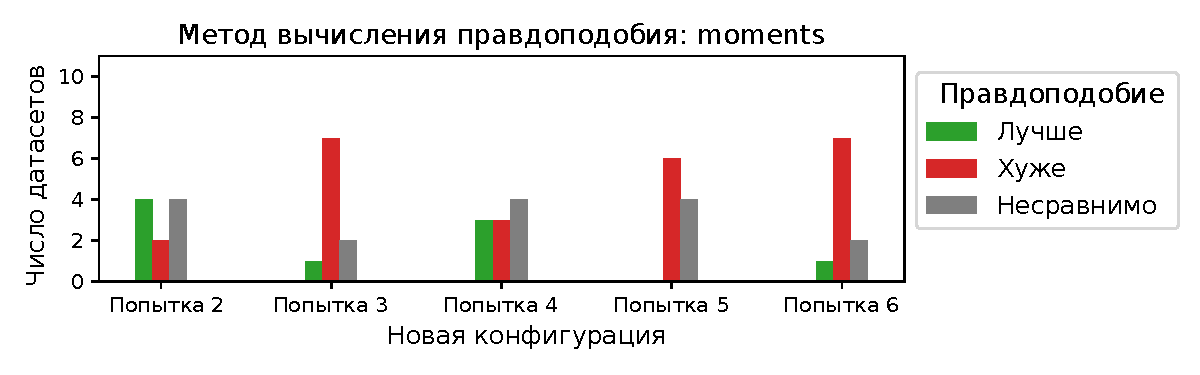
\includegraphics[width=.8\textwidth]{images/part2/genetics_algorithm/conf_comp_moments_rus.pdf}
    %\caption{}
    %\label{fig:part2:genetic_algorithm:HPO:ll_comp_moments}
    %\end{subfigure}
    %\begin{subfigure}[b]{.8\textwidth}
    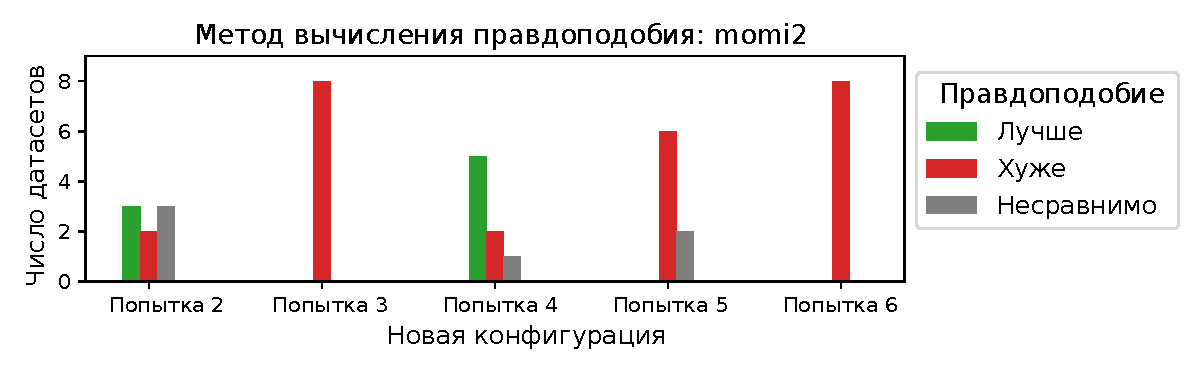
\includegraphics[width=.8\textwidth]{images/part2/genetics_algorithm/conf_comp_momi2_rus.pdf}
    %\caption{}
    %\label{fig:part2:genetic_algorithm:HPO:ll_comp_momi}
    %\end{subfigure}
    \caption{Сравнение значений правдоподобия, полученных с помощью новых конфигураций и исходной конфигурации генетического алгоритма}
    \label{fig:part2:genetic_algorithm:HPO:ll_comp}
\end{figure}

\begin{figure}[ht]
    \centering
    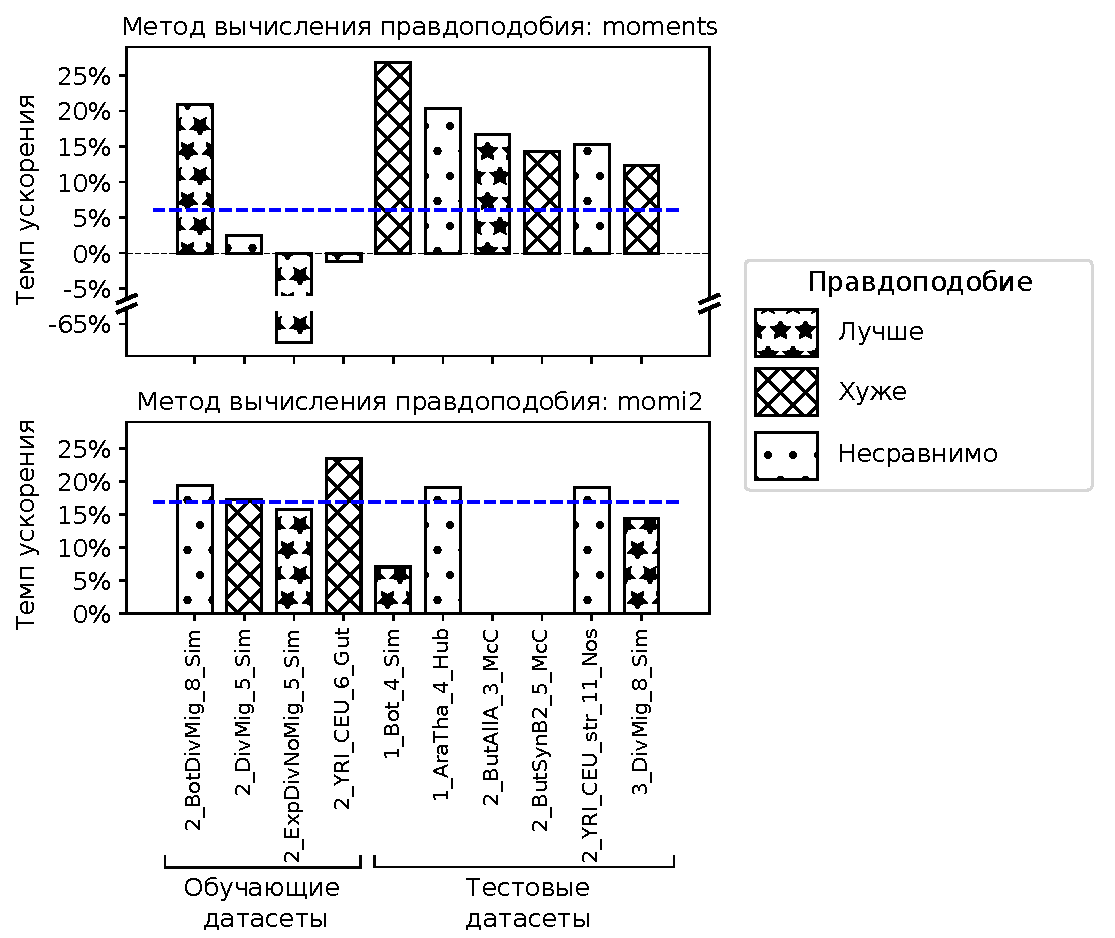
\includegraphics[width=0.8\textwidth]{images/part2/genetics_algorithm/GADMA2_comp_rus.pdf}
    \caption{Сравнение генетического алгоритма с настроенными гиперпараметрами с исходной версией на различных наборах данных}
    \label{fig:part2:genetic_algorithm:HPO:final_comp}
\end{figure}



\FloatBarrier
\section{Метод на основе комбинации байесовской оптимизации и локального поиска для настройки параметров модели демографической истории популяций по генетическим данным}
\label{sec:part2:bayesian_optimization}

%\subsection{Метод байесовской оптимизации}
%\label{sec:part2:bayesian_optimization:method}

\emph{Байесовская оптимизация} является одним из наиболее популярных методов для оптимизации сложных функций, которые не имеют заданной структуры, например, градиента, и требуют значительных вычислительных затрат~\cite{kushner1964new, movckus1975bayesian, mockus1989bayesian}.
Она направлена на минимизацию целевой функции ${f: \Theta \to \mathbb{R}}$, где для любого ${\theta \in \Theta}$ можно получить зашумленное наблюдение $y(\theta)$ для значения $f(\theta)$.
Целью оптимизации является быстрая и точная сходимость к глобальному оптимуму в рамках заданного временного бюджета.

Процедура байесовской оптимизации включает две основные компоненты: аппроксимацию целевой функции с использованием \textit{суррогатной модели} и выбор следующей точки для вычисления целевой функции с помощью \textit{функции выбора}.
Для суррогатной модели часто применяется регрессия на основе гауссовского процесса (подробнее об этом будет рассказано далее). %в разделе~\ref{sec:part2:bayesian_optimization:gp_regression}).
Гауссовские процессы имеют ряд преимуществ, включая способность работать с небольшим объемом данных и возможность количественной оценки неопределенности, связанной с аппроксимацией функции.
Кроме гауссовских процессов, в байесовской оптимизации иногда используются также случайные леса~\cite{hutter2011sequential}.
Например, они были применены в методе оптимизации гиперпараметров SMAC.
Тем не менее гауссовский процесс является наиболее распространенным выбором, и именно он был выбран в качестве суррогатной модели для байесовской оптимизации в данной работе.
Поэтому в данном разделе описание метода сразу предполагает использование гауссовского процесса.


\subsection{Разработка метода на основе комбинации байесовской оптимизации и локального поиска} 
\label{sec:part2:bayesian_optimization:development}

Процедура байесовской оптимизации начинается с построения начального множества решений и вычисления целевой функции на них.
Эта процедура называется \textit{начальным дизайном}.
После этого выбирается априорный гауссовский процесс.% (подробнее в разделе \ref{sec:part2:bayesian_optimization:gp_regression}).
Выбор априорного процесса может быть сделан на основе известных свойств целевой функции или с помощью процедуры кросс-валидации, которая подробно описана далее.% в разделе \ref{sec:part2:bayesian_optimization:cross-validation}.

На каждой итерации байесовской оптимизации строится регрессия на основе Гауссовского процесса на текущих точках $(\theta_1, y_1),\dots(\theta_n, y_n)$.
Затем на основе регрессии строится функция выбора, выбирается новая точка $\theta_*$, как точка ее максимума:
\[
\theta_* = \argmax_{\theta} \alpha(\theta),
\]
и происходит вычисление целевой функции в ней: $y_{n+1} = f(\theta^*)$.
Затем начинается новая итерация байесовской оптимизации.
Функция выбора в общем случае может быть произвольной, однако для обеспечения эффективности метода ее вычисление и оптимизация должны требовать меньше вычислительных ресурсов, чем вычисление целевой функции.

Наиболее часто используемые функции выбора~\cite{rasmussen2006}:
\begin{align}
    \label{eqn:acq_EI}
    \alpha_{\mathrm{EI}}(\theta) &= \mathbb{E}\bigl[\max\bigl(0, \min_{1 \leq i \leq n}(y_i) - \hat{f}(\theta)\bigr)\bigr],
    \\
    \label{eqn:acqPI}
    \alpha_{\mathrm{PI}}(\theta) &= \mathbb{P}\bigl[\hat{f}(\theta) < \min_{1 \leq i \leq n}(y_i)\bigr],
    \\
    \label{eqn:acq_logEI}
    \alpha_{\mathrm{logEI}}(\theta) &= \mathbb{E}\bigl[\max(0, \min_{1 \leq i \leq n}(e^{y_i}) - e^{\hat{f}(\theta)})\bigr],
\end{align}
где $\hat{f}$ --- аппроксимация целевой функции $f$ суррогатной моделью.
Функция выбора $\alpha_{\mathrm{EI}}$ (EI, Expected Improvement) оценивает ожидаемое улучшение --- максимально возможное ожидаемое улучшение целевой функции в точке.
Функция выбора $\alpha_{\mathrm{PI}}$ (PI, Probability of Improvement) моделирует вероятность \emph{любого} улучшения по сравнению с текущим оптимумом.
Функция выбора $\alpha_{\texttt{logEI}}(\theta)$, была предложена в~\cite{hutter2009experimental} и является аналогом функции выбора \texttt{EI}, когда аппроксимация $\hat{f}$ суррогатной моделью использует логарифмированные значения целевой функции $f$.
Это означает, что регрессия строится на точках $(\theta_i, \log y_i)$, вместо точек $(\theta_i, y_i)$.
Логарифмирование требует, чтобы целевая функция принимала только положительные значения --- $y_j > 0$.
Целевая функция $f$, используемая в данной работе --- отрицательный логарифм правдоподобия, который всегда имеет положительное значение, поэтому функцию выбора $\alpha_{\texttt{logEI}}(\theta)$ можно использовать.
Для суррогатной модели гауссовского процесса рассматриваемые функции выбора представляются в аналитическом виде и могут быть эффективно оптимизированы с использованием алгоритмов градиентного спуска с перезапусками.
Далее в тексте функции выбора \eqref{eqn:acq_EI}, \eqref{eqn:acqPI} и \eqref{eqn:acq_logEI} будут обозначаться, как \texttt{EI}, \texttt{PI} и \texttt{LogEI} соответственно.

\begin{figure}[b]
    \centering
    \begin{subfigure}{.31\textwidth}
      \centering
      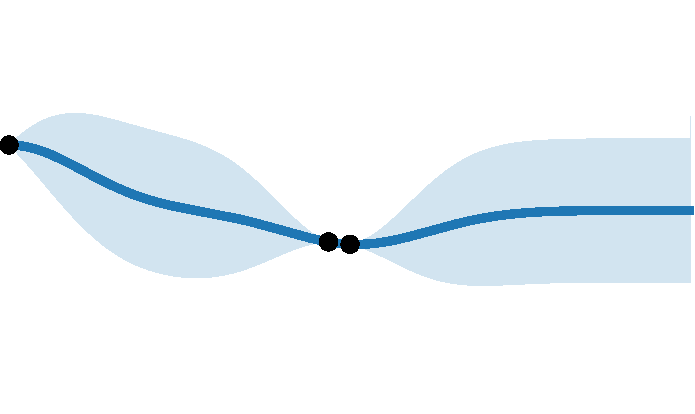
\includegraphics[width=\textwidth]{images/part2/bayesian_optimization/iter_3.pdf}
      \caption{}
      \label{fig:part2:bayesian_optimization:bo_1}
    \end{subfigure}%
    \hspace{0.03\textwidth}%
    \begin{subfigure}{.31\textwidth}
      \centering
      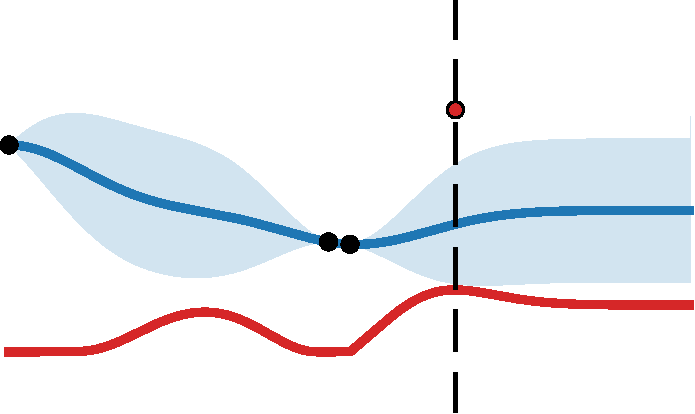
\includegraphics[width=\textwidth]{images/part2/bayesian_optimization/iter_4.pdf}
      \caption{}
      \label{fig:part2:bayesian_optimization:bo_2}
    \end{subfigure}%
    \hspace{0.03\textwidth}%
    \begin{subfigure}{.31\textwidth}
      \centering
      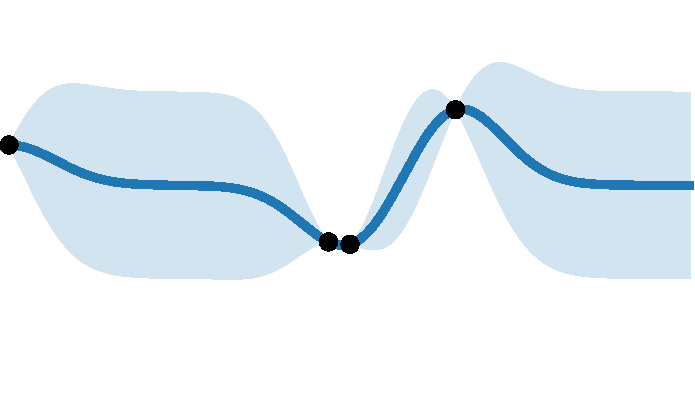
\includegraphics[width=\textwidth]{images/part2/bayesian_optimization/iter_5.pdf}
      \caption{}
      \label{fig:part2:bayesian_optimization:bo_3}
    \end{subfigure}
    \caption{Фрагмент байесовской оптимизации}
    \label{fig:part2:bayesian_optimization:bo}
\end{figure}

Пример итерации байесовской оптимизации изображен на рисунке~\ref{fig:part2:bayesian_optimization:bo}.
Голубая линия соответствует предсказанию регрессии на основе гауссовского процесса, голубая область вокруг --- доверительный интервал предсказания.
Красная линия соответствует функции выбора, пунктирная черная линия --- точке ее максимума.
Рисунок~\ref{fig:part2:bayesian_optimization:bo_1} изображает начало итерации, когда происходит построение регрессии на основе гауссовского процесса по черным точкам, где была вычислена целевая функция.
Затем происходит поиск точки максимума функции выбора, изображенной красной линией на рисунке~\ref{fig:part2:bayesian_optimization:bo_2}, и вычисление целевой функции в ней --- красная точка. 
Наконец, рисунок~\ref{fig:part2:bayesian_optimization:bo_3} демонстрирует как текущее множество точек обновляется и новая регрессия строится на его основе.

Псевдокод процедуры байесовской оптимизации представлен в листинге~\ref{alg:part2:bayesian_optimization}.
Алгоритм принимает на вход целевую функцию $f$, которая является функцией правдоподобия, начальное множество точек $X^{init}$, суррогатную модель гауссовского процесса $GP$, функцию выбора $\alpha$ и максимальное число итераций $T^{max}$.

\begin{algorithm}[ht]
\caption{Псевдокод метода байесовской оптимизации}
\label{alg:part2:bayesian_optimization}
\begin{algorithmic}[1]
\Function{BayesianOptimization}{$f, X^{\text{init}}, \text{GP}, \alpha, T^{\max}$}
    \State {$Y^{\text{init}} \leftarrow \{f(\theta),\ \theta \in X^{\text{init}}\}$}
    \State {$X, Y \leftarrow X^{\text{init}}, Y^{\text{init}}$}
    \State {$T_{\text{cur}} \leftarrow 1$}
    \While{$T_{\text{cur}} \leq T^{\max}$}
        \State {$\text{GP} \leftarrow \Call{GaussianProcessRegression}{\text{GP}, X, Y}$}
        \State {$\alpha_{\text{GP}} \leftarrow \Call{GetAcquisitionFunctionForGP}{\text{GP}}$}
        \State {$\theta^\star \leftarrow \arg\max_\theta \alpha_{\text{GP}}(\theta)$}
        \State {$X \leftarrow X \cup \{\theta^\star\}$}
        \State {$Y \leftarrow Y \cup \{f(\theta^\star)\}$}
    \EndWhile
\State \Return $\theta_{\text{best}}:\ \arg\max_{\theta \in X} f(\theta)$
\EndFunction
\end{algorithmic}
\end{algorithm}


Для решения задачи настройки параметров моделей демографической истории по генетическим данным был разработан комбинированный метод байесовской оптимизации и локального поиска.
Как и в случае с генетическим алгоритмом, разработанный метод последовательно запускает сначала байесовскую оптимизацию для настройки всех параметров, а затем метод локальной оптимизации для дополнительной настройки непрерывных параметров.
Схема алгоритма разработанного метода представлена на рисунке~\ref{fig:part2:bayesian_optimization:scheme}.

\begin{figure}[b]
  \centering
   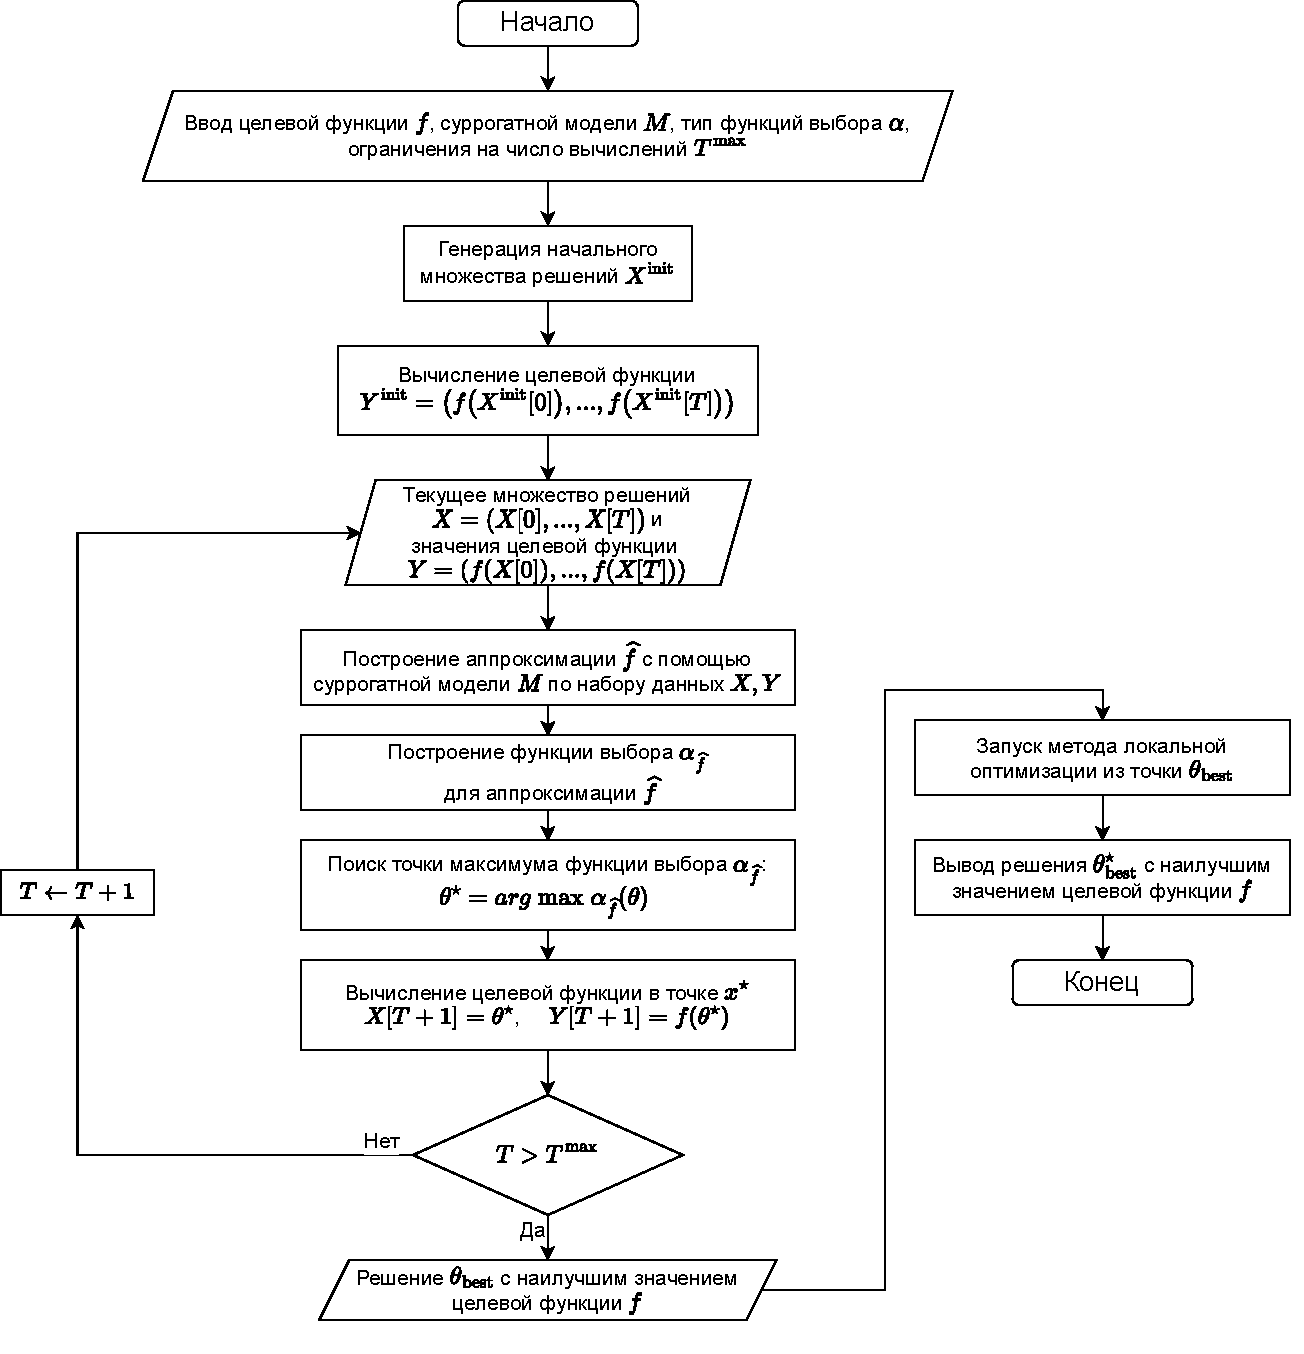
\includegraphics[width=\linewidth]{images/part2/bayesian_optimization/bayesian_optimization_scheme.drawio.pdf}
   \caption{Схема алгоритма разработанного комбинированного метода, основанного на баейсовской оптимизации и методе локального поиска}
  \label{fig:part2:bayesian_optimization:scheme}
\end{figure}

Для выбора функции выбора и гиперпараметров суррогатной модели в байесовской оптимизации были проведены экспериментальные исследования для выявления эффективности различных конфигураций.
Был также разработан и протестирован метод автоматического выбора функции ковариации суррогатной модели гауссовского процесса.
В результате было предложено применение ансамблевого метода байесовской оптимизации в составе разработанного комбинированного метода.
Этот метод включает разработанный метод автоматического выбора функции ковариации, а также ансамбль из функций выбора.
На каждой итерации байесовской оптимизации функция выбора выбирается случайным образом из этого ансамбля.
Подробное описание настройки гиперпараметров байесовской оптимизации приведено в разделе~\ref{sec:part2:bayesian_optimization:overview}.\\


\textbf{Регрессия на основе гауссовского процесса.} 
%\label{sec:part2:bayesian_optimization:gp_regression}
С математической точки зрения, \emph{гауссовский процесс} --- это семейство~${\{\hat{f}_\theta\}_{\theta \in \mathcal{\Theta}}}$ случайных величин  $\hat{f}_\theta$, проиндексированных множеством $\Theta \subset \mathbb{R}^d$  и распределенных согласно многомерному гауссовскому распределению.
Следовательно, для любого конечного множества индексов $\theta_1, \theta_2, \dots, \theta_k$ множества $\Theta$ случайная величина:
$$\hat{f}_{\theta_1, \dots, \theta_k} = (\hat{f}_{\theta_1}, \dots, \hat{f}_{\theta_k})$$
имеет многомерное нормальное распределение $\hat{f}_{\theta_1, \dots, \theta_k} \sim \mathcal{N}_k(\mu,\, K^{2})$.

Гауссовский процесс или, строго говоря, его распределение определяется парой детерминистических функций: функцией среднего ${m: \Theta \to \mathbb{R}}$ и функцией ковариации $k: \Theta \times \Theta \to \mathbb{R}$:
\begin{align}
    &m(\theta) = \mathbb{E}(\hat{f}_\theta), & & k(\theta, \theta') = Cov(\hat{f}_{\theta}, \hat{f}_{\theta'}).
\end{align}
Функция ковариации $k$ также называется \textit{ядром} гауссовского процесса.

Было доказано, что любая пара функций $m$ и $k$, где $k$ --- положительно определенная функция, определяет гауссовский процесс~\cite{rasmussen2006}, из этого следует стандартное обозначение:
\begin{equation}
    \hat{f} \sim GP(m, k).
\end{equation}

\FloatBarrier

Для процедуры регрессии на основе гауссовского процесса требуется выбрать \emph{параметры априорного распределения} $\hat{f}_{0} \sim GP(m, k)$.
На практике функция среднего $m$ обычно предполагается равной нулю или другой константе~\cite{rasmussen2006}.
В разработанной байесовской оптимизации для настройки параметров моделей демографической истории используется $m  \equiv 0$, что позволяет сосредоточиться больше на выборе ковариационной функции $k$.

Наиболее распространенное семейство ковариационных функций для гауссовского процесса --- \emph{семейство ядер Матерна} \cite{stein2012,rasmussen2006}.
В контексте данной работы понятие ядра равнозначно понятию ковариационной функции гауссовского процесса.
Семейство ядер Матерна параметризовано тремя гиперпараметрами: \emph{гладкость} $\nu$, \emph{масштаб} $\kappa$ и \emph{дисперсия} $\sigma^2$.
Гладкость определяет степень дифференцируемости гауссовского процесса, масштаб и дисперсия масштабируют оси значений параметров и целевой функции.
Предполагая нулевой априорный вектор средних, общий вид ядер Матерна выглядит следующим образом~\cite{gradshteyn2014}:

\begin{equation} \label{eqn:matern_general}
k_{\nu, \kappa, \sigma^2}(t, t^\prime)
\!=\!
\frac{2^{1-\nu}}{\Gamma(\nu)}
\left(
  \sqrt{2 \nu}
  \frac{\|t-t^\prime\|}{\kappa}
\right)^{\nu}
\!\!\!
K_\nu\left(
  \sqrt{2 \nu}
  \frac{\|t-t^\prime\|}{\kappa}
\right),
\end{equation}
где $K_{\nu}$ --- это функция Бесселя второго порядка, а $\Gamma$ --- гамма-функция.

Семейство ядер Матерна, заданное формулой~\eqref{eqn:matern_general}, часто делят на подсемейства, соответствующие выбору гладкости $\nu$.
Наиболее используемыми являются подсемейства для $\nu \in \{1/2, 3/2, 5/2, \infty\}$, что приводит к получению следующих формул:
\begin{align}
\label{eqn:matern12}
k_{1/2, \kappa, \sigma^2}(t, t^\prime)
&=
\sigma^2 \exp\left(-\frac{u}{\kappa}\right),
\\
\label{eqn:matern32}
k_{3/2, \kappa, \sigma^2}(t, t^\prime)
&=
\sigma^2 \left(1+\frac{\sqrt{3}u}{\kappa}\right)\exp\left(-\frac{\sqrt{3}u}{\kappa}\right),
\\
\label{eqn:matern52}
k_{5/2, \kappa, \sigma^2}(t, t^\prime)
&=
\sigma^2 \left(1+\frac{\sqrt{5}u}{\kappa} + \frac{5 u^2}{3 \kappa^2}\right)\exp\left(-\frac{\sqrt{5}u}{\kappa}\right),
\\
\label{eqn:rbf}
k_{\infty, \kappa, \sigma^2}(t, t^\prime)
&=
\sigma^2 \exp\left(-\frac{u^2}{2 \kappa^2}\right),
\end{align}
где $u = \|t-t'\|$. Первое ядро $k_{1/2, \kappa, \sigma^2}$ обычно называется \emph{экспоненциальным}, последнее $k_{\infty, \kappa, \sigma^2}$ --- \emph{гауссовским} ядром или ядром \emph{RBF}.

% На рисунке~\ref{fig:part2:bayesian_optimization:gp_kernel} показано, как изменяется среднее и доверительный интервал гауссовского процесса при изменении гиперпараметров ядра RBF.
% Крестообразными точками изображена обучающая выборка.
% Синей линией на графиках изображена средняя функция $m$ гауссовского процесса, а голубая область отображает $95\%$-ный доверительный интервал, соответствующий ковариационной функции $k_{\infty, \kappa, \sigma^2}$.
% Рисунок~\ref{fig:part2:bayesian_optimization:gp_kernel:variance} демонстрирует, что при увеличении дисперсии $\sigma^2$ увеличивается вертикальное изменение траектории функции и погрешность моделирования исходных точек аппроксимации.
% Значение масштаба $\kappa$ на рисунке~\ref{fig:part2:bayesian_optimization:gp_kernel:variance} влияет на форму средней функции.
% При малом значении масштаба функция стремится быть константной и равной нулю.
% При увеличении гиперпараметра $\kappa$ функция может быть отлична от нуля.

% \begin{figure}[ht]
%     \begin{subfigure}{\textwidth}
%     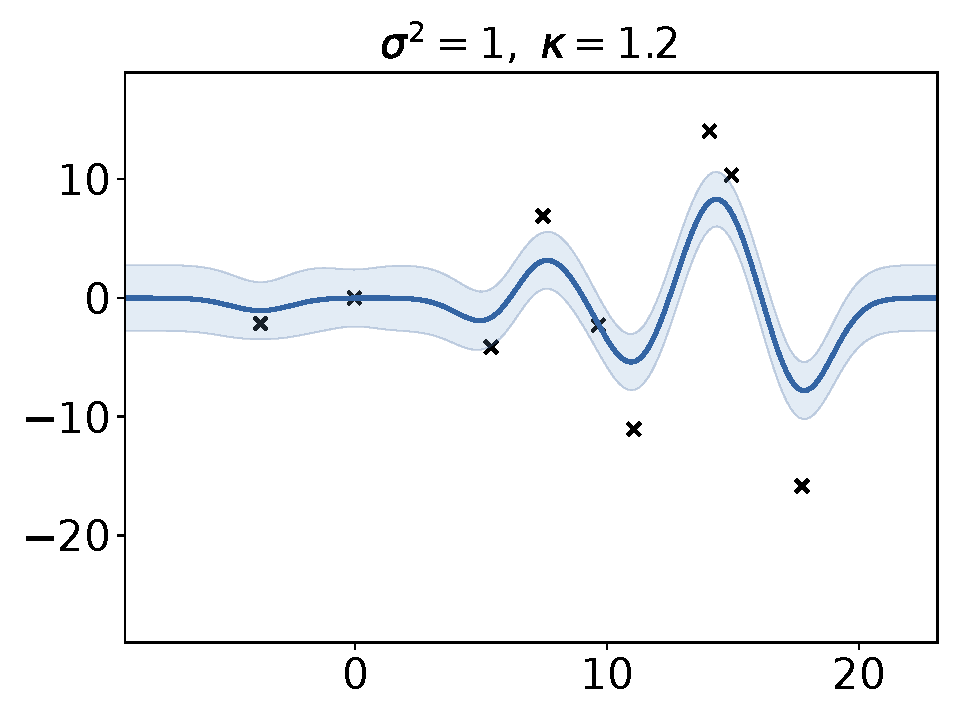
\includegraphics[width=0.33\linewidth]{images/part2/bayesian_optimization/gp_regression/sigma_1_kappa_1.2.pdf}
%     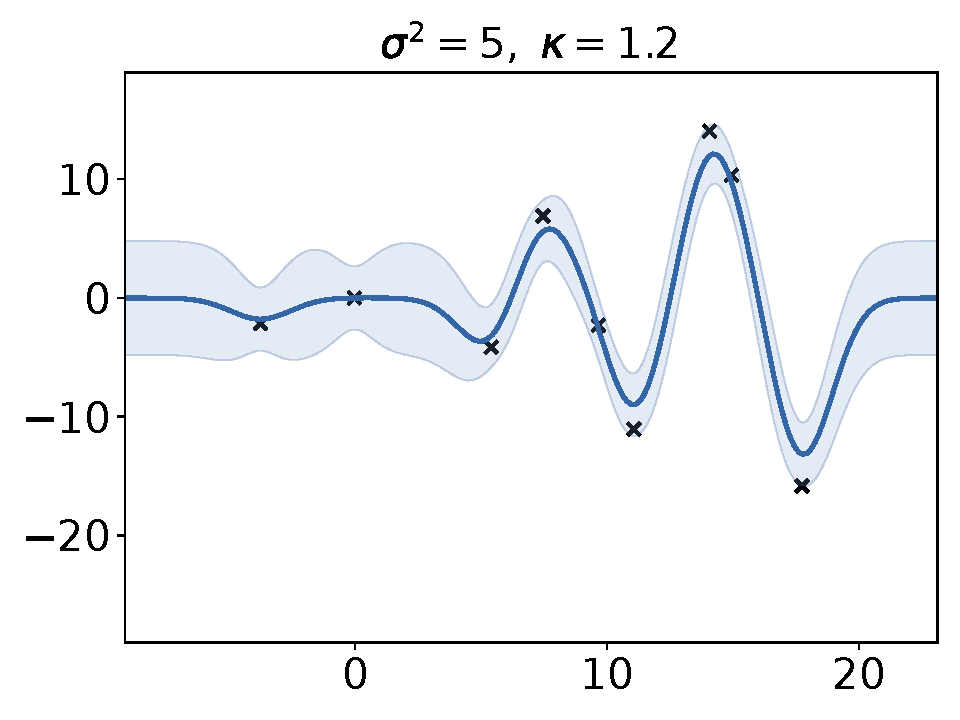
\includegraphics[width=0.33\linewidth]{images/part2/bayesian_optimization/gp_regression/sigma_5_kappa_1.2.pdf}
%     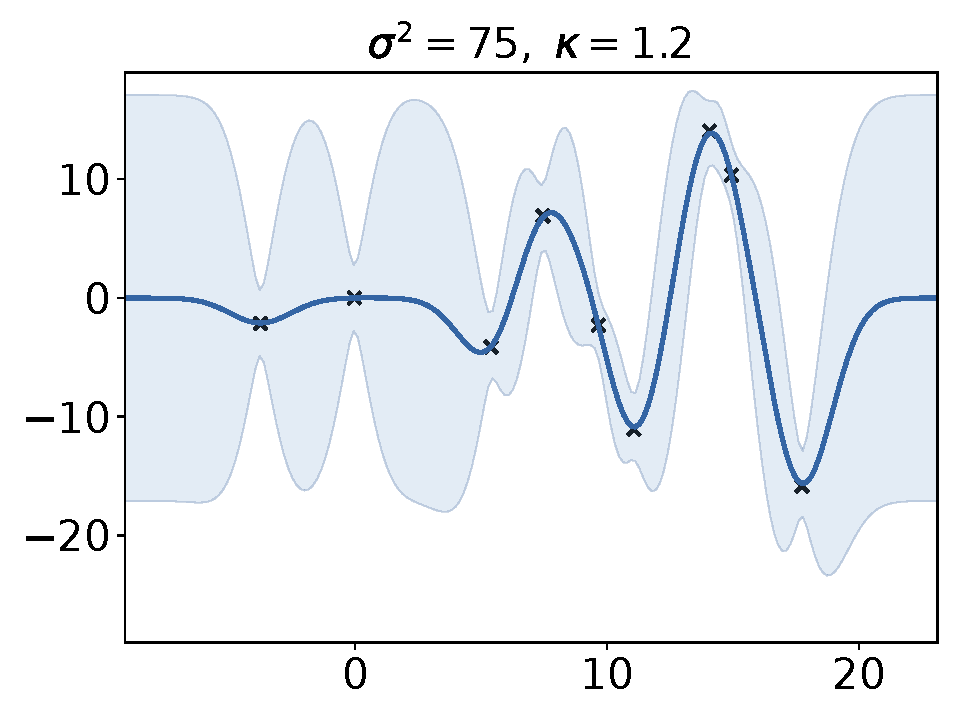
\includegraphics[width=0.33\linewidth]{images/part2/bayesian_optimization/gp_regression/sigma_75_kappa_1.2.pdf}
%     \caption{Различные значения дисперсии $\sigma^2=\{1, 5, 75\}$ при фиксированном масштабе~${\kappa=1.2}$}
%     \label{fig:part2:bayesian_optimization:gp_kernel:variance}
%     \end{subfigure}
%     \begin{subfigure}{\textwidth}
%     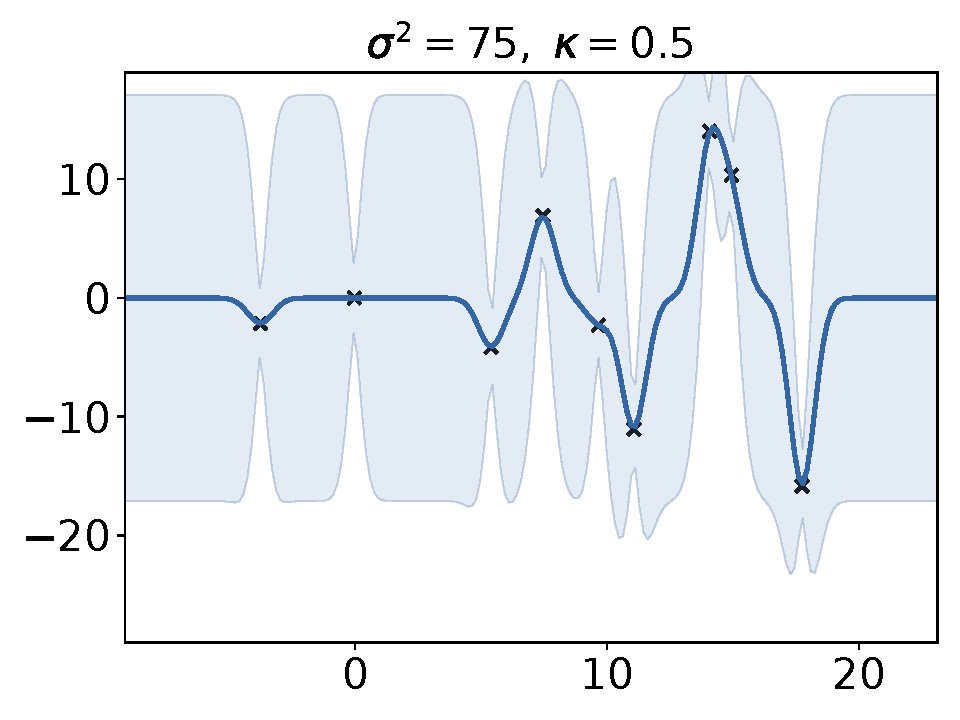
\includegraphics[width=0.33\linewidth]{images/part2/bayesian_optimization/gp_regression/sigma_75_kappa_0.5.pdf}
%     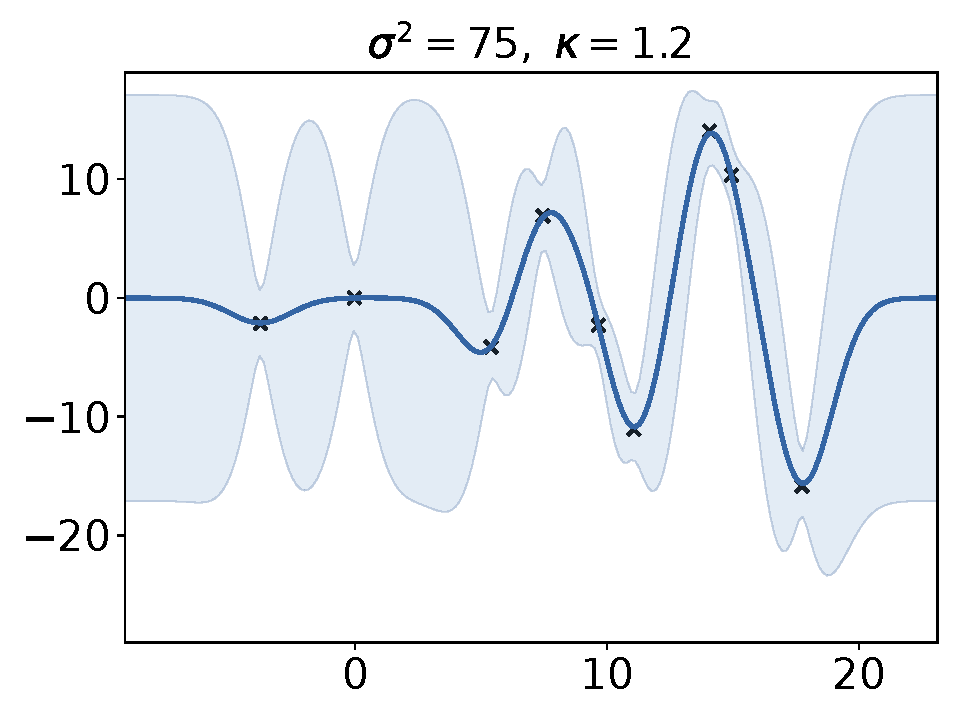
\includegraphics[width=0.33\linewidth]{images/part2/bayesian_optimization/gp_regression/sigma_75_kappa_1.2.pdf}
%     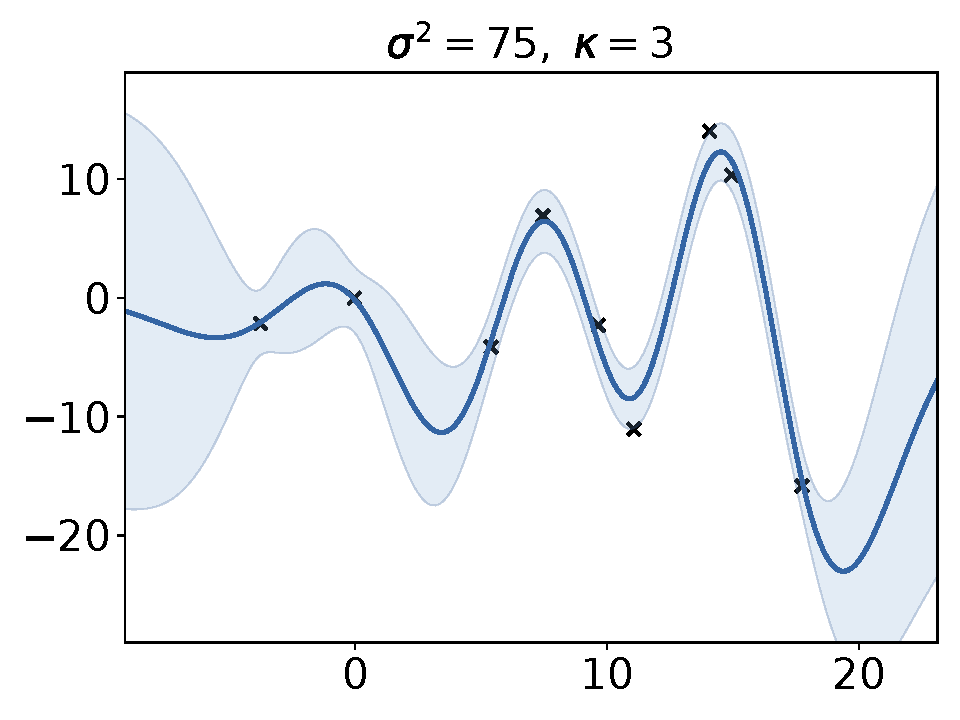
\includegraphics[width=0.33\linewidth]{images/part2/bayesian_optimization/gp_regression/sigma_75_kappa_3.pdf}
%     \caption{Различные значения масштаба $\kappa=\{0.5, 1.2, 3.0\}$ при фиксированной дисперсии~${\sigma^2=75}$}
%     \label{fig:part2:bayesian_optimization:gp_kernel:lengthscale}
%     \end{subfigure}
% \caption{Пример изменения регрессии на основе гауссовского процесса при изменении гиперпараметров его RBF ядра $k_{\infty, \kappa, \sigma^2}$}
% \label{fig:part2:bayesian_optimization:gp_kernel}
% \end{figure}


Аппроксимирующая часть предложенной байесовской оптимизации использует \emph{регрессию на основе гауссовского процесса}.
Имея априорный гауссовский процесс $\hat{f}_0$ и набор точек $(\theta_1, y_1), \dots, (\theta_n, y_n)$, можно построить апостериорный гауссовский процесс $\hat{f}$, используя формулу Байеса:
\begin{equation} \label{eqn:bayes}
p(\hat{f})
\stackrel{\text{def}}{=}
p(\hat{f} | \v{y})
=
\frac{p(\v{y} | \hat{f}_0) p(\hat{f}_0)}{p(\v{y})},
\end{equation}
где $\v{y} = (y_1, \ldots, y_n)^{\top}$. В общем случае апостериорное распределение не всегда является гауссовским процессом.
Однако, если предположить, что каждое наблюдение $y_i$ зашумлено $y_i = f(\theta_i) + \varepsilon$, где $\varepsilon \sim N(0, \sigma_{\varepsilon}^2)$, то $\hat{f}$ всегда является гауссовским процессом~\cite{rasmussen2006}.
Более того, $\hat{f} \sim GP(\hat{m}, \hat{k})$ с функциями  $\hat{m}$ и $\hat{k}$, полученными следующим образом (для простоты предполагаем, что $m \equiv 0$):
\begin{align}
\hat{m}(\cdot)
    &= \m{K}_{\cdot,\v{\theta}}(\m{K}_{\v{\theta},\v{\theta}} + \sigma_{\varepsilon}^{2}\m{I})^{-1}\v{y},
\label{eqn:gp_mean}
\\
\hat{k}(\cdot, \cdot')
    &=k(\cdot, \cdot') - \m{K}_{\cdot,\v{\theta}}(\m{K}_{\v{\theta},\v{\theta}} + \sigma_{\varepsilon}^{2}\m{I})^{-1}\m{K}_{\v{t}, \cdot'},
\label{eqn:gp_var}
\end{align}
где для пары векторов $\v{a} \in \Theta^l, \v{b} \in \Theta^s$ символ $\m{K}_{\v{a}, \v{b}}$ обозначает $l \times s$ матрицу, определенную как $\left(\m{K}_{\v{a}, \v{b}}\right)_{i j} = k(\v{a}_i, \v{b}_j)$; $\v{\theta} = (\theta_1, \ldots, \theta_n)^{\top}$, а $\v{y} = (y_1, \ldots, y_n)^{\top}$.

Регрессия на основе гауссовского процесса требует выбора функции среднего и ковариационной функции --- ядра.
Регрессия выполняется в два этапа.
На первом из них происходит поиск оптимальных гиперпараметров $\hat{\lambda}$ ковариационной функции $k$ и дисперсии шума $\hat{\sigma_{\varepsilon}}^2$, дающих максимальное значение правдоподобия $\log p_{\lambda, \sigma_{\varepsilon}^2}(\v{y})$~\cite{rasmussen2006}:
\[
\begin{split}
\hat{\lambda}, \hat{\sigma_{\varepsilon}}^2
=
\argmax_{\lambda, \sigma_{\varepsilon}^2}
&\log p_{\lambda, \sigma_{\varepsilon}^2}(\v{y}) =
\\
=
\argmax_{\lambda, \sigma_{\varepsilon}^2}
\bigg\{&-\frac{1}{2}\v{y}^{\top}(\m{K}_{\lambda, \v{\theta}, \v{\theta}} + \sigma_{\varepsilon}^2 \m{I})^{-1} \v{y}
\ - \\
&-\frac{1}{2}\log\left(\det\left(\m{K}_{\lambda, \v{\theta}, \v{\theta}} + \sigma_{\varepsilon}^2 \m{I}\right)\right)
-\frac{n}{2}\log(2\pi)\bigg\}.
\end{split}
\]
Для решения этой оптимизационной задачи обычно используют градиентный спуск с перезапусками.

Вторым этапом регрессии на основе гауссовского процесса является вычисление разложения Холецкого~\cite{benoit1924note} для обращения положительно определенной матрицы
$(\m{K}_{\hat{\lambda}, \v{\theta},\v{\theta}} + \hat{\sigma}_{\varepsilon}^{2}\m{I})$, что эквивалентно решению следующей линейной системы:
\begin{equation}
(\m{K}_{\hat{\lambda}, \v{\theta},\v{\theta}} + \hat{\sigma}_{\varepsilon}^{2}\m{I}) \, \v{a} = \v{b}.
\end{equation}

После этого апостериорное среднее $\hat{m}(x)$ и функцию ковариации $\hat{k}(x, x)$ можно вычислить по формулам~\ref{eqn:gp_mean} и \ref{eqn:gp_var}.

Задача оптимизации, включающая решение линейной системы и вычисление определителя, а также последующий шаг вычисления разложения Холецкого имеют вычислительную сложность $\mathrm{O}(n^3)$, где $n$ --- размер точек, где была вычислена целевая функция.
Поиск $\hat{\lambda}, \hat{\sigma_n}^2$ требуется на каждой итерации процедуры оптимизации, что делает ее узким местом вычислительной сложности метода регрессии.
Это не позволяет использовать этот простой подход при больших $n$.
Однако вычисление функций среднего и ковариации имеют оценки $\mathrm{O}(n)$ и $\mathrm{O}(n^2)$ соответственно и легко распараллеливаемы.


\textbf{Кросс-валидация для выбора параметров априорного гауссовского процесса.} %\label{sec:part2:bayesian_optimization:cross-validation}
Параметры априорного гауссовского процесса такие, как функции среднего и ковариации, часто выбираются вручную, основываясь на знаниях свойств аппроксимируемой функции.
Однако есть способ выполнить этот выбор автоматически с использованием процедуры \emph{кросс-валидации}.
Для фиксированного конечного набора значений параметров эта процедура позволяет выбрать наилучшие значения с помощью метрики $L_{\mathrm{LOO-CV}}$ качества регрессии.
Процедура кросс-валидации была использована при настройке гиперпараметров комбинированного метода, основанного на байесовской оптимизации и локальном поиске. 

Пусть имеются данные $\{(\theta_i, y_i)\}_{i=1}^n$ для построения регрессии.
Для вычисления метрики $L_{\mathrm{LOO-CV}}$ последовательно перебираются точки $\theta_i$ и для каждой происходит построение регрессии гауссовского процесса $\hat{f}_{-i}$ по данным $\v{\theta}_{-i}, \v{y}_{-i}$ с исключенной точкой $\theta_i$.
Для построенной регрессии вычисляется значение функции $Q(y_i, \hat{f}_{-i}(\theta_i))$, которая оценивает качество предсказания $\hat{f}_{-i}(\theta_i)$ в исключенной точке $\theta_i$.
Метрика $L_{\mathrm{LOO-CV}}$ регрессии гауссовского процесса с заданными параметрами определяется, как усреднение значений $Q(y_i, \hat{f}_{-i}(\theta_i))$:
\[
L_{\mathrm{LOO-CV}}
=
\frac{1}{n}
\sum_{i=1}^n
Q(y_i, \hat{f}_{-i}(\theta_i)).
\]
При этом чем больше значение $L_{\mathrm{LOO-CV}}$, тем лучше качество регрессии.

Функция качества $Q$ может быть определена разными способами.
Например, если предположить, что $\hat{f}_{-i}(\theta_i) = N(\mu, \sigma^2)$, то $Q$ может быть определена следующим образом:
\[
Q(y_i, \hat{f}_{-i}(t_i))
=
- \mathbb{E} (y_i - \hat{f}_{-i}(t_i))^2
= - (y_i - \mu)^2 - \sigma^2.
\]
Однако метрика $L_{\mathrm{LOO-CV}}$ с такой функцией качества будет отдавать предпочтение тем регрессиям, которые более уверены в своем прогнозе: меньшее значение $\sigma^2$ напрямую приводит к большему значению $Q$.
В связи с этим была использована другая функция оценки качества предсказания, которая способна лучше сбалансировать качество предсказания со степенью уверенности~\cite{rasmussen2006}:
\begin{equation}
Q(y_i, \hat{f}_{-i}(t_i))
=
\log p_{\hat{f}_{-i}(t_i)}(y_i)
=
- \frac{(y_i - \mu)^2}{2\sigma^2}
- \frac{1}{2} \log(2 \pi \sigma^2).
\label{eqn:log_likelihood}
\end{equation}
%В данной работе для процедуры кросс-валидации используется метрика $L_{\mathrm{LOO-CV}}$ с функцией качества $Q$, определенной по формуле~\eqref{eqn:log_likelihood}.
В случаях, когда используется функция выбора \texttt{LogEI}, значение~$y_i$ в~формуле~\eqref{eqn:log_likelihood} заменяется на $\log y_i$.

\subsection{Реализация разработанного метода, основанного на комбинации байесовской оптимизации и локального поиска}
\label{sec:part2:bayesian_optimization:implementation}

Для реализации разработанного метода, основанного на комбинации байесовской оптимизации и локального поиска, был расширен модуль \texttt{optimizers} добавлением классов для баейсовской оптимизации.
Модуль \texttt{optimizers} был разработан для реализации  аналогичного комбинированного метода на основе генетического алгоритма. Его описание доступно в разделе~\ref{sec:part2:genetic_algorithm:implementation}.

Выделим несколько готовых к использованию библиотек, реализующих байесовскую оптимизацию: GPyOpt~\cite{gpyopt2016}, BOTorch~\cite{balandat2020botorch} и SMAC~\cite{hutter2011sequential, lindauer2022smac3}. 
Они включают реализацию различных суррогатных моделей, например, гауссовских процессов, и функций выбора, которые необходимы при разработке и реализации байесовской оптимизации.
Библиотека GPyOpt была одной из широко применяемых библиотек, однако она не поддерживается с 2020 года.
Библиотека BOTorch была создана в 2020 году и все еще продолжает активно развиваться.
Библиотека SMAC, предложенная в 2011 году, успела хорошо зарекомендовать себя в ряде приложений \cite{lago2018forecasting, hewamalage2021recurrent, wu2022nflat} и, что важно, реализует функцию выбора $\alpha_{logEI}$~\cite{hutter2009experimental}, которая используется в данной работе.
Поэтому для реализации байесовской оптимизации была использована библиотека SMAC~v0.13.1.

Два класса \texttt{SMACBayesianOptimizer} \texttt{SMACBOEnsemble} были разработаны и интегрированы в модуль \texttt{optimizers} для реализации байесовской оптимизации.
На рисунке~\ref{fig:part2:bayesian_optimization:implementation:classes} изображена обновленная структура класса, добавленные классы выделены более жирными линиями.

\begin{figure}[ht]
    \centering
    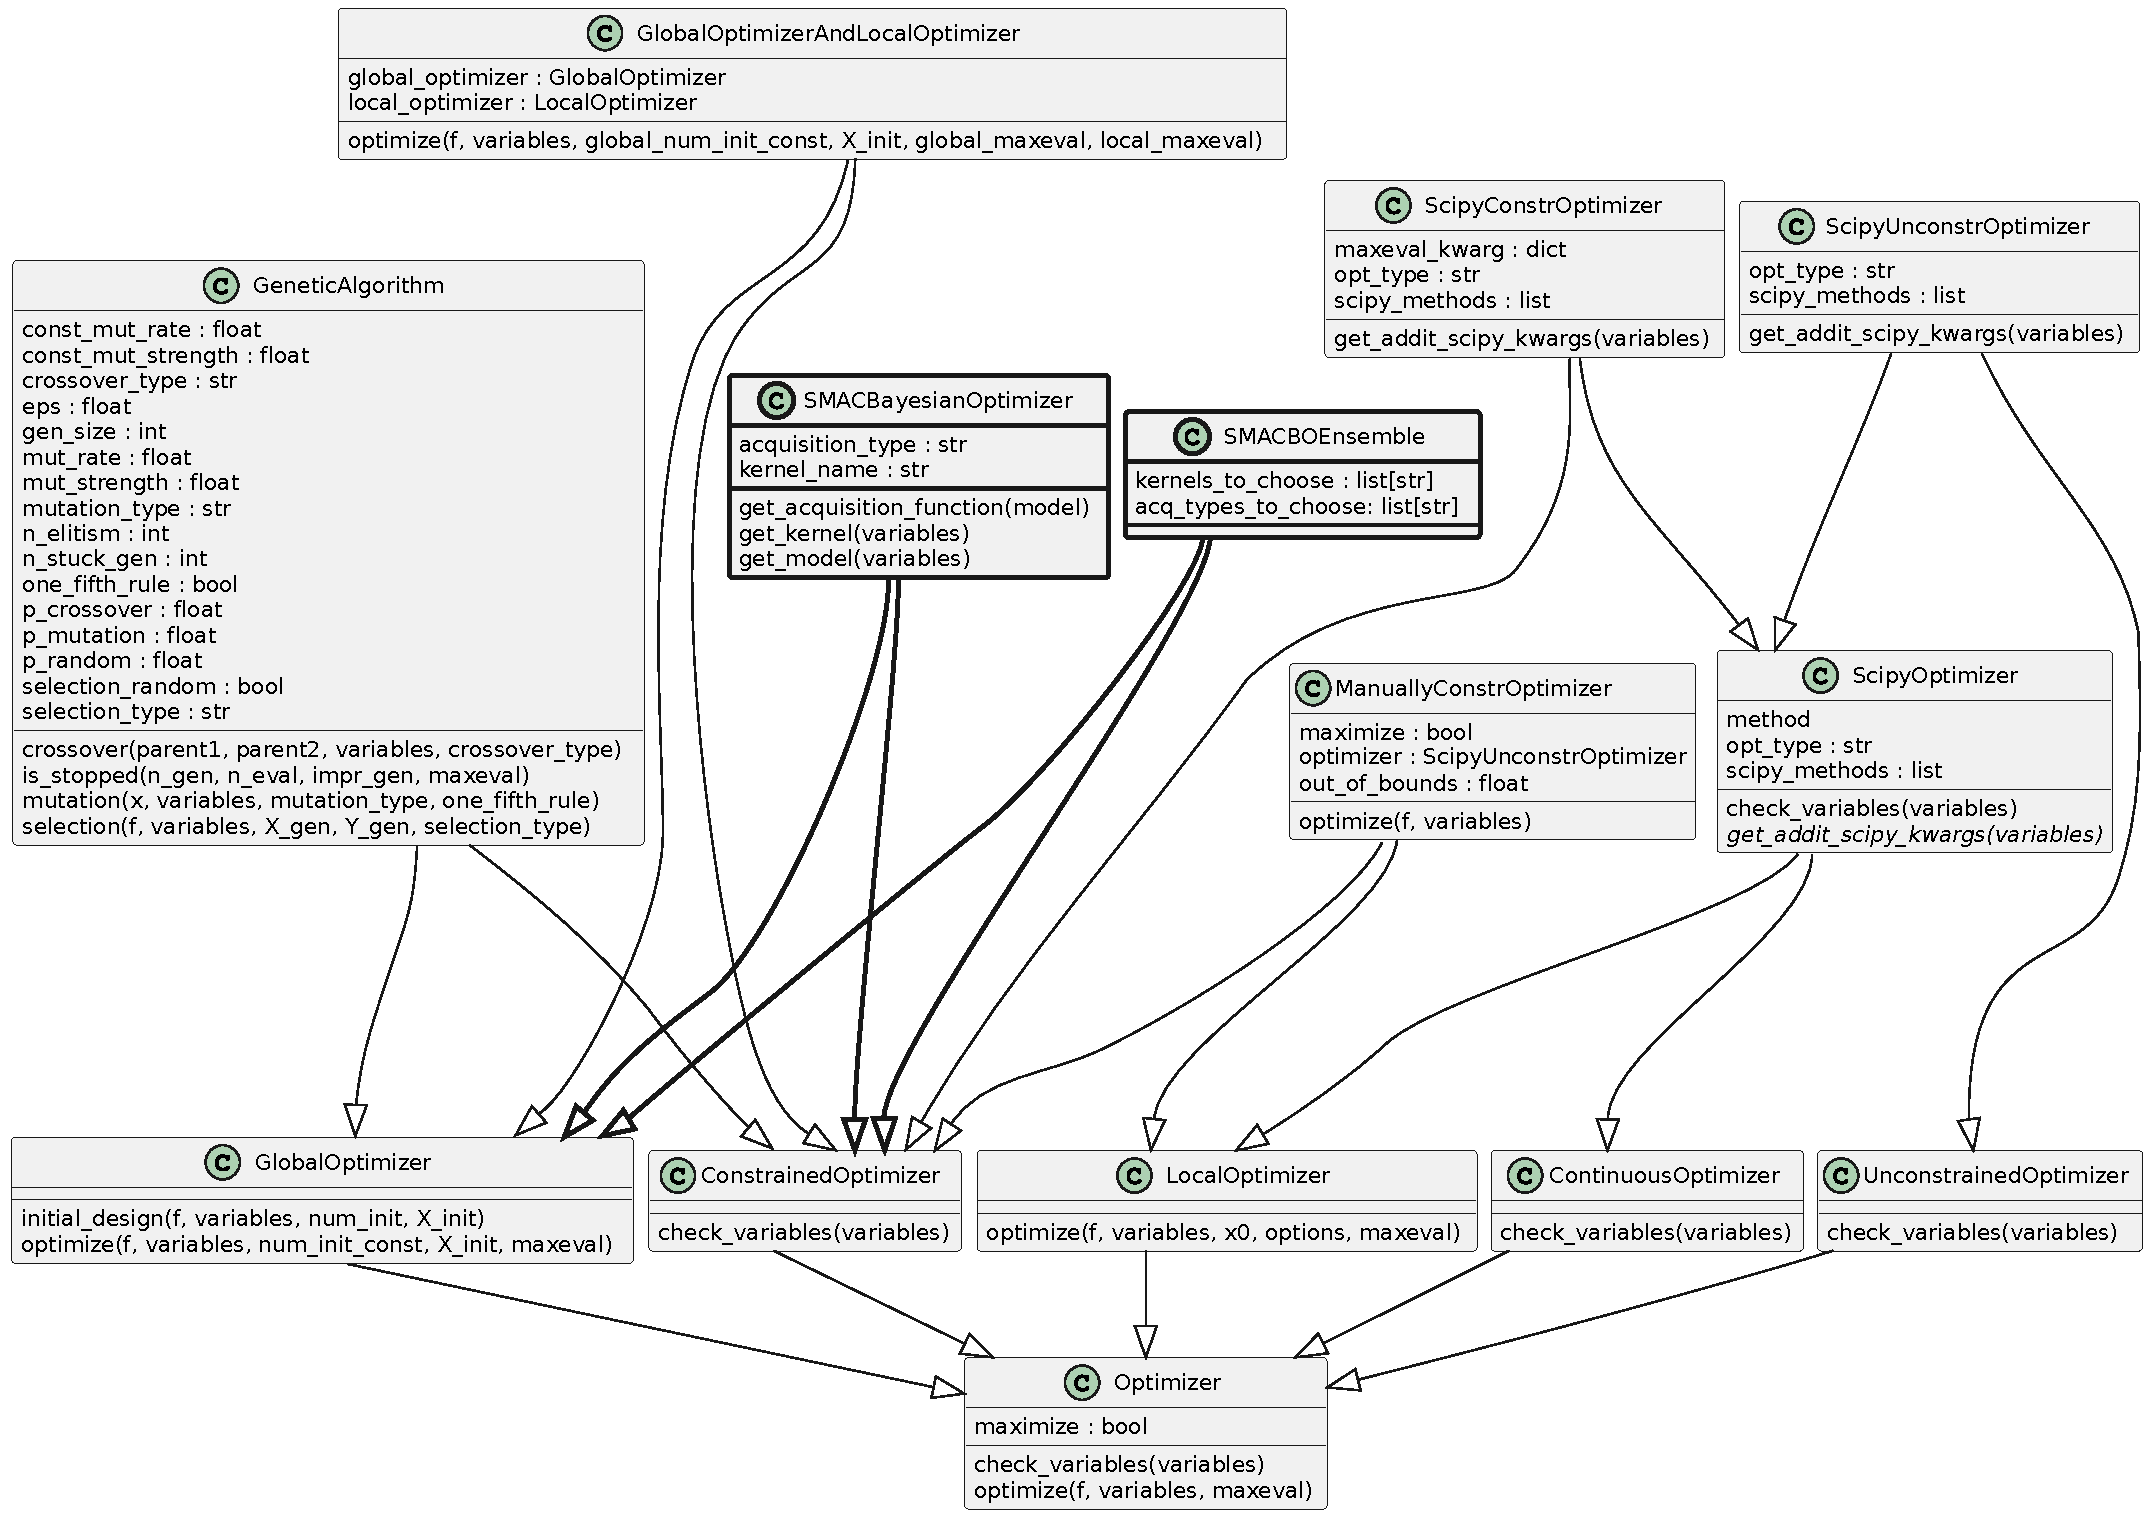
\includegraphics[width=\linewidth]{images/part5/optimizer_classes_short.pdf}
    \caption{Обновленная структура классов модуля \texttt{optimizers}}
    \label{fig:part2:bayesian_optimization:implementation:classes}
\end{figure}

Класс \texttt{SMACBayesianOptimizer} реализует байесовскую оптимизацию с гауссовским процессом в качестве суррогатной модели.
Он требует выбранных функции ковариации (атрибут \texttt{kernel\_type}) и функции выбора (атрибут \texttt{acquision\_type}).
Пример создания байесовской оптимизации с ковариационной функцией, заданной ядром Матерна с гладкостью $\nu= 5/2$, и функцией выбора $\alpha_{EI}$, представлен на рисунке~\ref{fig:part2:bayesian_optimization:implementation:bo}.
Дополнительно, класс \texttt{SMACBayesianOptimizer} реализует метод автоматического выбора ковариационной функции, что применяется в случае, если атрибут \texttt{kernel\_type} объекта выбран равным \texttt{"Auto"}.
Пример создания байесовской оптимизации с функцией выбора $\alpha_{PI}$ и функции ковариации, которая выбирается автоматически, также представлен на рисунке~\ref{fig:part2:bayesian_optimization:implementation:bo}.

\begin{figure}[ht]
    \centering
    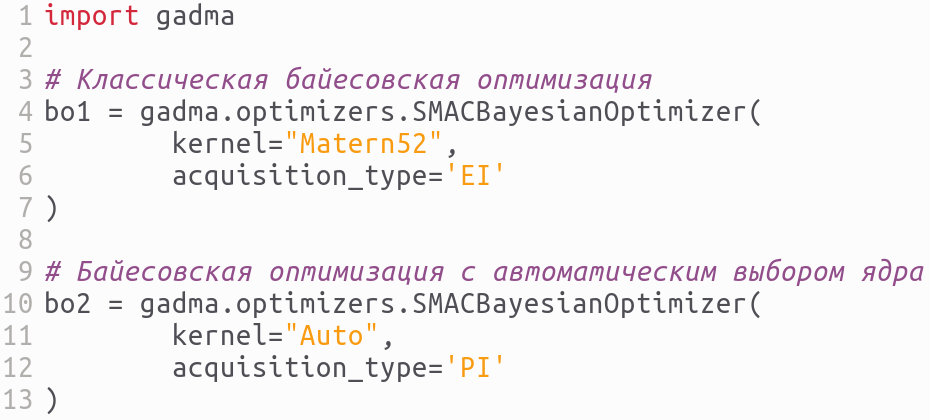
\includegraphics[width=0.8\linewidth]{images/part2/bayesian_optimization/bo_implementation.png}
    \caption{Обновленная структура классов модуля \texttt{optimizers}}
    \label{fig:part2:bayesian_optimization:implementation:bo}
\end{figure}

Класс \texttt{SMACBOEnsemble} реализует ансамблевую байесовскую оптимизацию.
Атрибут \texttt{kernels\_to\_choose} является списком доступных функций ковариации гауссовского процесса для автоматического выбора.
По умолчанию метод выбирает из двух функций: ядро Матерна с гладкостью $\nu=5/2$ и ядро RBF.
Атрибут \texttt{acq\_types\_to\_choose} является списком функций выбора, включенных в ансамбль, по умолчанию рассматриваются две функции выбора: $\alpha_{PI}$ и $\alpha_{LogEI}$
Подробное описание причин выбора этих функций будет приведено в разделе~\ref{sec:part2:bayesian_optimization:overview}.

Как и в случае с генетическим алгоритмом, \textbf{разработанный комбинированный метод} на основе байесовской оптимизации и локального поиска реализован, как объект класса \texttt{GlobalOptimizerAndLocalOptimizer}.
Однако, в качестве метода глобальной оптимизации используется ансамблевая байесовская оптимизация --- объект класса \texttt{SMACBOEnsemble}.
Пример реализации разработанного метода представлен на рисунке~\ref{fig:part2:bo_implementation:rosenbrock_ex}, где дополнительно продемонстрировано применение этого метода для поиска точки минимума функции Розенброка~\cite{rosenbrock1960automatic}.
Пример вывода этой программы представлен на рисунке~\ref{fig:part2:bo_implementation:rosenbrock_out}.

\begin{figure}[ht]
    \centering
    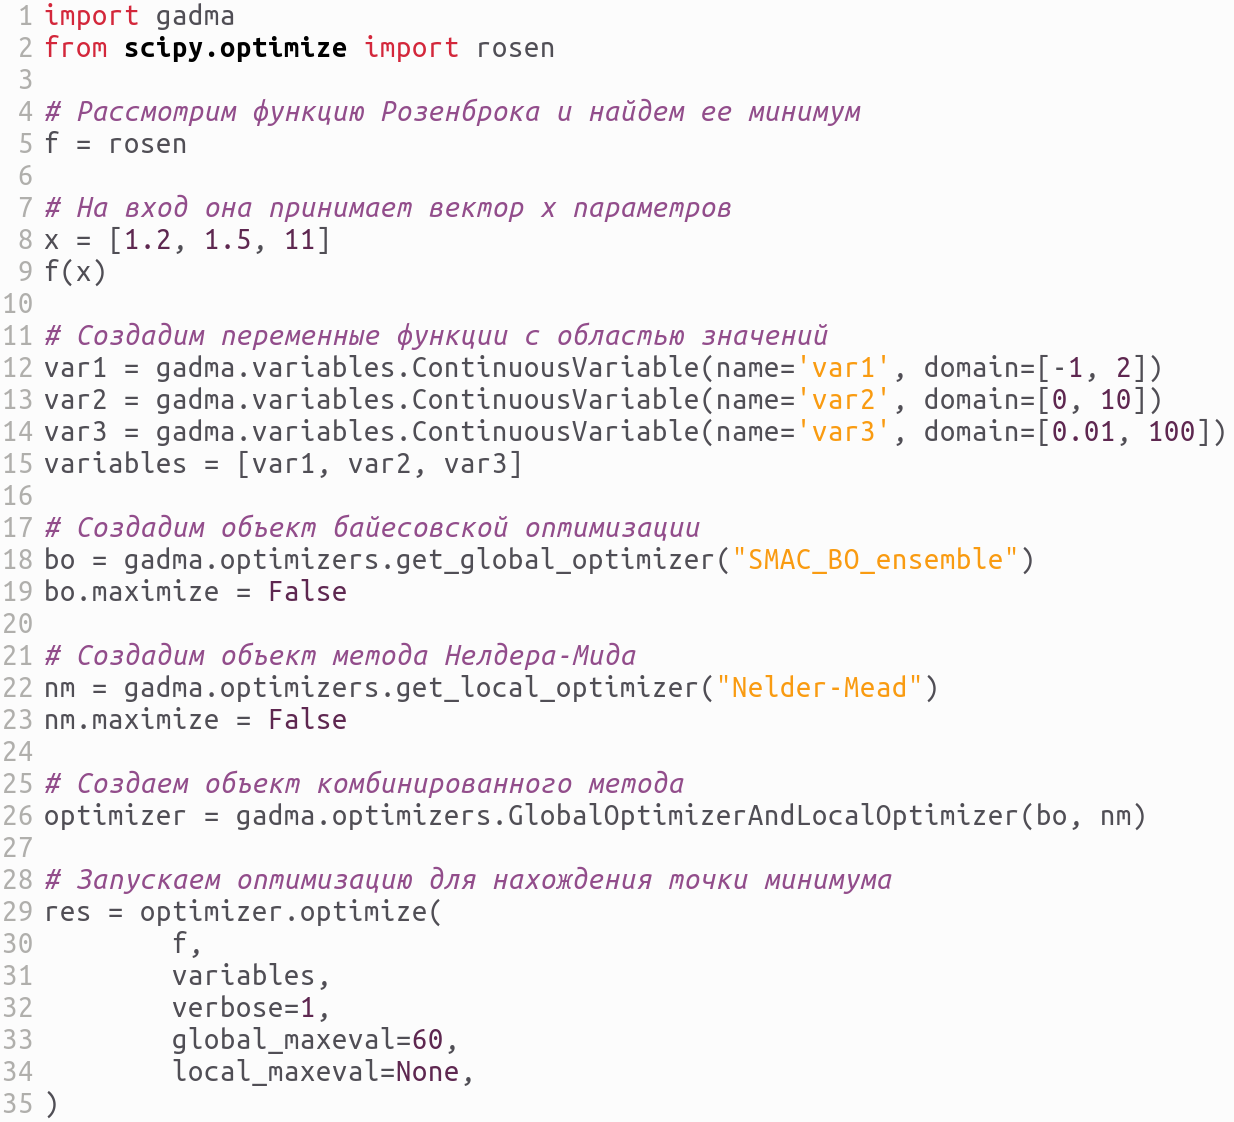
\includegraphics[width=\linewidth]{images/part2/bayesian_optimization/example_run_bo.png}
    \caption{Применение разработанного комбинированного метода на основе байесовской оптимизации, реализованного с помощью модуля \texttt{optimizers}, для поиска точки минимума функции Розенброка}
    \label{fig:part2:bo_implementation:rosenbrock_ex}
\end{figure}

\begin{figure}[ht]
    \centering
    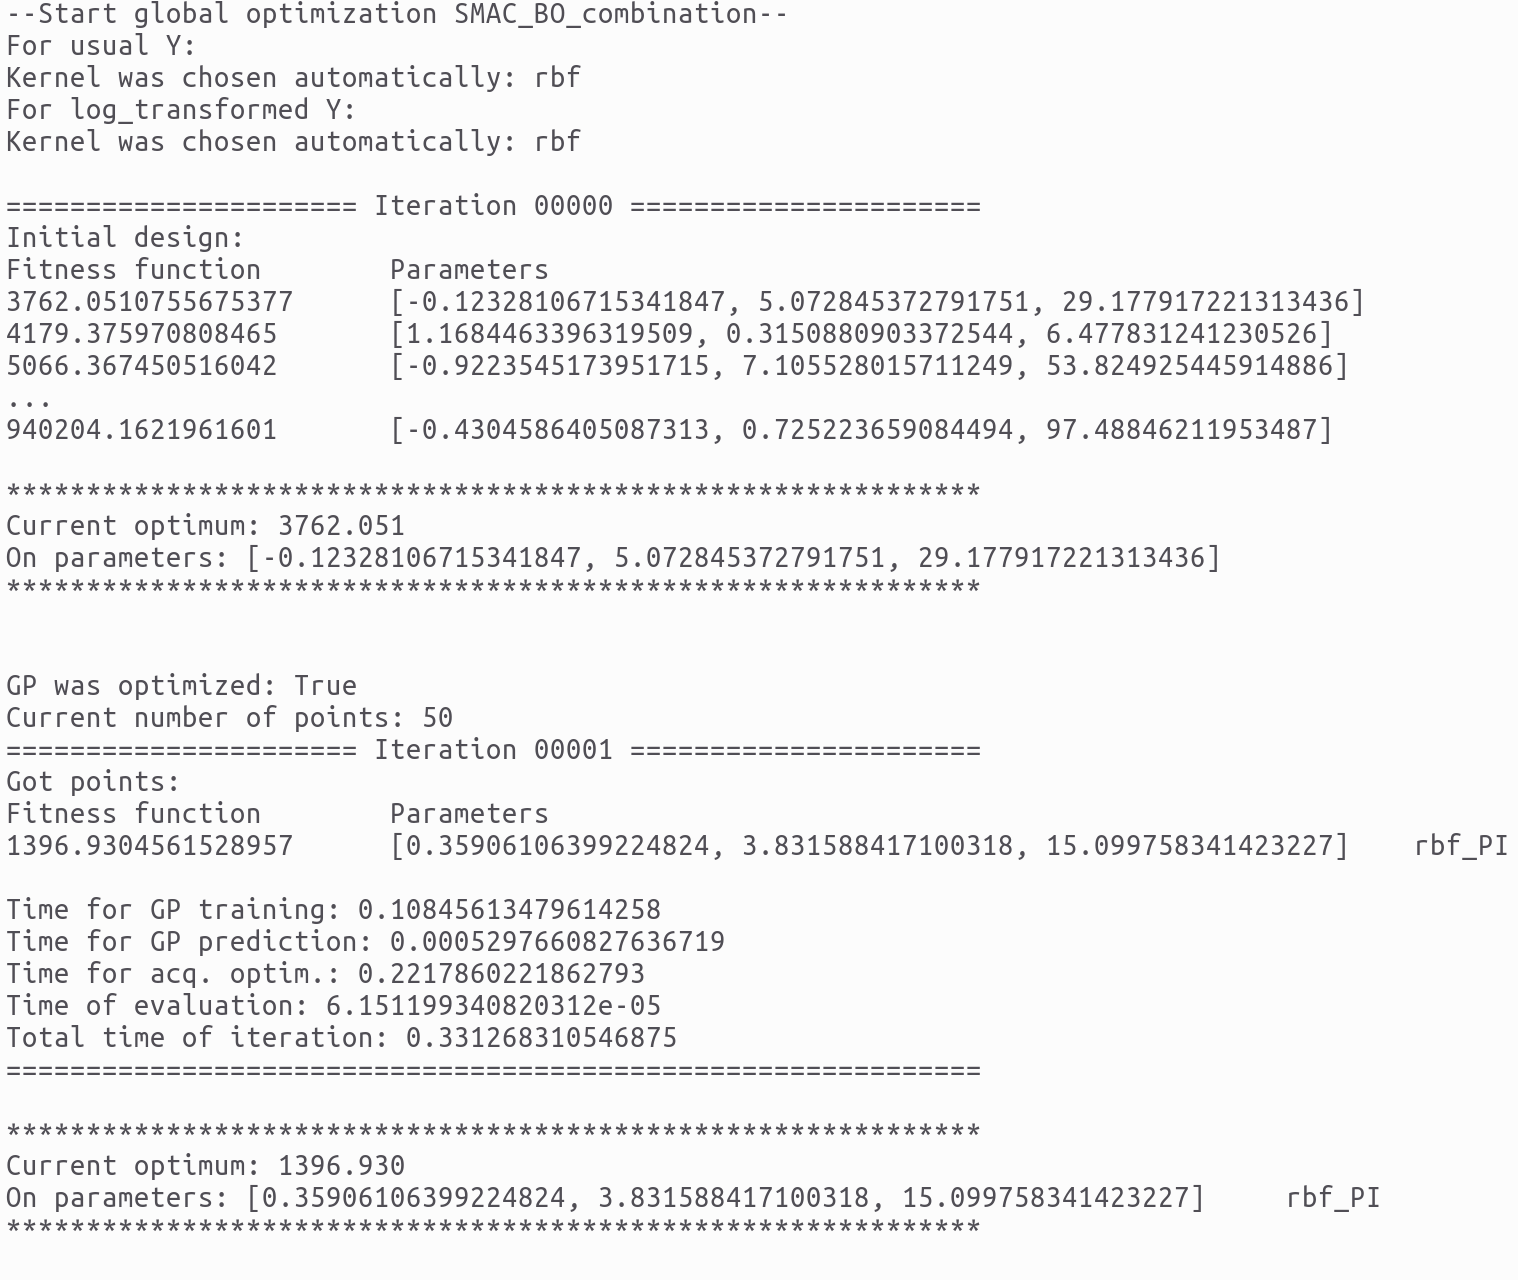
\includegraphics[width=0.85\linewidth]{images/part2/bayesian_optimization/bo_output.png}
    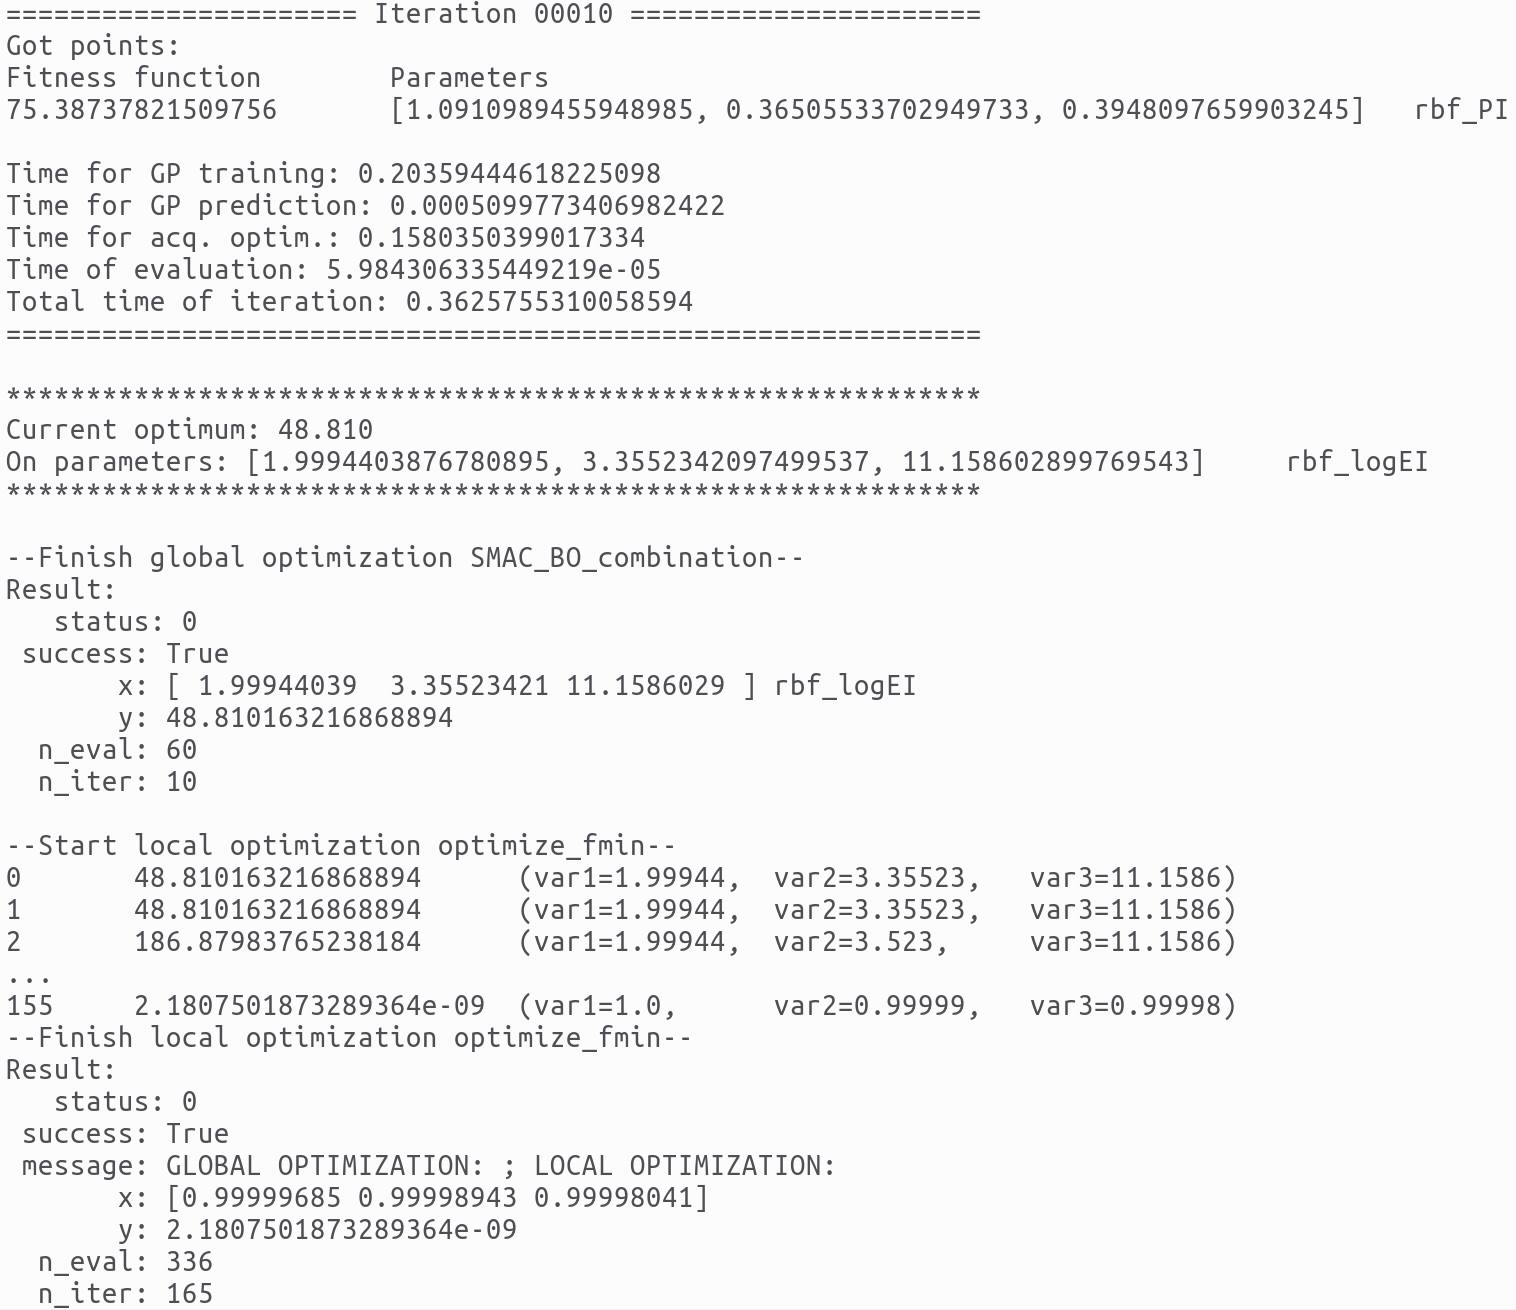
\includegraphics[width=0.85\linewidth]{images/part2/bayesian_optimization/ls_bo_output.png}
    \caption{Пример вывода программы, представленной на рисунке~\ref{fig:part2:bo_implementation:rosenbrock_ex}}
    \label{fig:part2:bo_implementation:rosenbrock_out}
\end{figure}

\FloatBarrier
\subsection{Настройка гиперпараметров байесовской оптимизации и разработка ансамблевого метода}
\label{sec:part2:bayesian_optimization:overview}

Для решения задачи поиска параметров $\theta$ модели $\mathcal{M}$ демографической истории популяций на основе генетических данных $\mathfrak{D}$ было разработано несколько методов, основанных на байесовской оптимизации.
Для априорного гауссовского процесса ранее было предложено использовать функцию среднего $m(\theta) \equiv 0$.
В таких предположениях метод байесовской оптимизации включает два неизвестных гиперпараметра: 1) функцию ковариации гауссовского процесса и 2) функцию выбора.
%Были разработаны несколько методов, проведены экспериментальные исследования для этих методов и конфигураций их гиперпараметров, на основе которых был разработан финальный метод байесовской оптимизации для решения задачи вывода демографической истории.
Сначала была выполнена процедура кросс-валидации для оценки качества регрессии гауссовского процесса, построенной на $2{\,}000$ точках при разных ковариационных функциях.
Затем были проведены экспериментальные исследования различных методов байесовской оптимизации на множестве наборов данных.
Методы были сравнены с использованием графиков сходимости, и были определены гиперпараметры, обеспечивающие наилучшую сходимость.
Сначала был рассмотрен метод классической байесовской оптимизации, который описан в разделе~\ref{sec:part2:bayesian_optimization}.
Была выявлена эффективность этого метода при различных конфигурациях двух рассматриваемых гиперпараметров.
Затем был разработан метод байесовской оптимизации с автоматическим выбором ядра гауссовского процесса и были сравнены его конфигурации с разными функциями выбора.
Наконец, на основе проведенных экспериментальных исследований был разработан ансамблевый метод с гиперпараметрами, который показал наилучшую производительность.
Было продемонстрировано, что ансамблевый метод является наиболее эффективным среди всех разработанных методов байесовской оптимизации.

Для вычисления правдоподобия был использован метод, реализованный в библиотеке \moments.
Для экспериментальных исследований было использовано одиннадцать наборов данных из пакета \texttt{deminf\_data v1.0.0}, который ранее использовался для настройки гиперпараметров генетического алгоритма (раздел~\ref{sec:part2:genetic_algorithm:hpo}) и доступен по ссылке \url{https://github.com/noscode/demographic_inference_data}.
Каждый набор данных содержит генетические данные в виде аллель-частотного спектра, модель демографической истории и границы для параметров модели.
Названия наборов данных имеют структуру, которая была приведена ранее на рисунке~\ref{fig:part2:genetic_algorithm:HPO:datasets}.
Список использованных наборов данных вместе с соответствующим временем вычисления правдоподобия представлен на рисунке~\ref{fig:part2:bo_hpo:eval_time_data_sets}.
Ось ординат представлена в логарифмической шкале.
Диаграммы размаха для времени вычисления правдоподобия, представленные на рисунке, окрашены в соответствии с их медианными значениями.

\begin{figure}[ht]
    \centering
    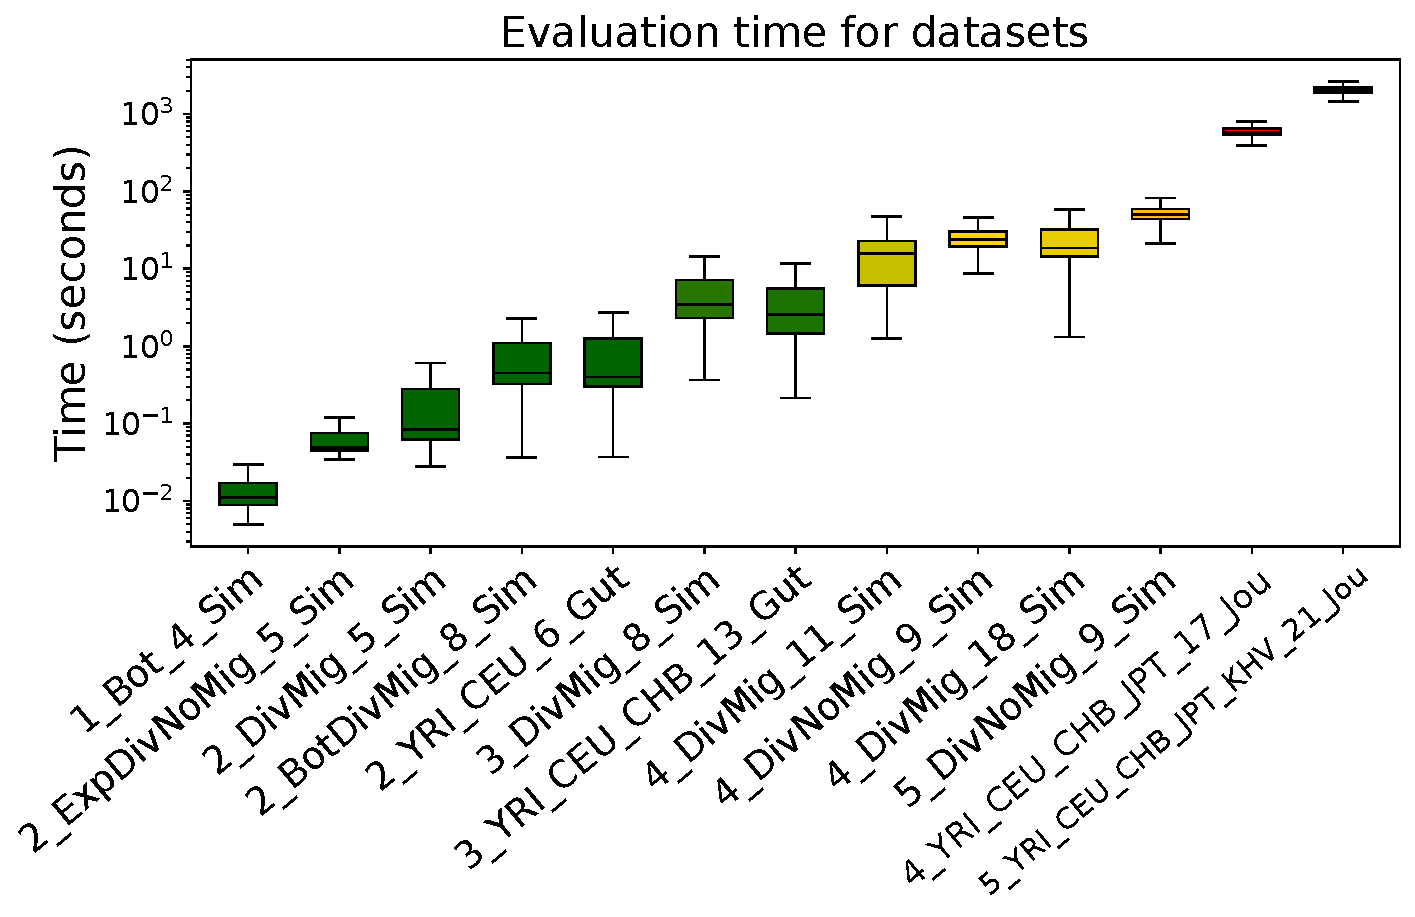
\includegraphics[width=\linewidth]{images_experiments/bo_hpo/eval_time_all_datasets.pdf}
    \caption{Время вычисления логарифма правдоподобия с помощью \moments для тестируемых наборов данных из пакета \texttt{deminf\_data v1.0.0}}
    \label{fig:part2:bo_hpo:eval_time_data_sets}
\end{figure}

Сравнение методов байесовской оптимизации в этом разделе было проведено на первых одиннадцати наборах данных.
Среди них присутствует один набор данных для одной популяции, четыре набора для двух популяций, два набора для трех популяций, три набора для четырех популяций и один набор данных для пяти популяций.
Два последних набора данных (\texttt{4\_YRI\_CEU\_CHB\_JPT\_17\_Jou} и \texttt{5\_YRI\_CEU\_CHB\_JPT\_KHV\_21\_Jou}) были использованы для сравнения ансамблевого метода байесовской оптимизации с генетическим алгоритмом и будут описаны далее.

Эффективность метода байесовской оптимизации зависит от выбора гиперпараметров --- ковариационной функции гауссовского процесса и функции выбора.
Были рассмотрены три функции выбора:
\begin{enumerate}
    \item Функция ожидаемого улучшения $\alpha_{EI}$ (Expected Improvement, \texttt{EI}),
    \item Функция вероятности улучшения $\alpha_{PI}$ (Probability of Improvement, \texttt{PI}),
    \item Функция ожидаемого улучшения для логарифмированных значений целевой функции $\alpha_{logEI}$ (Log Expected Improvement, \texttt{LogEI}).
\end{enumerate}
Были рассмотрены четыре функции ковариации гауссовского процесса:
\begin{enumerate}
    \item Экспоненциальное ядро $k_{1/2}$ (\texttt{Exponential}).
    \item Ядро Матерна $k_{3/2}$ с гладкостью $\nu=3/2$ (\texttt{Matern32}).
    \item Ядро Матерна $k_{5/2}$ с гладкостью $\nu=5/2$ (\texttt{Matern52}).
    \item Гауссовское ядро или ядро RBF $k_{\infty}$ (\texttt{RBF}).
\end{enumerate}

Одним из популярных способов выбора ядра гауссовского процесса для байесовской оптимизации является процедура кросс-валидации (LOO-CV), описанная в разделе~\ref{sec:part2:bayesian_optimization:development}.%\ref{sec:part2:bayesian_optimization:cross-validation}.
Четыре ядра гауссовского процесса были сравнены на одиннадцати наборах данных с использованием метрики $L_{LOO-CV}$, полученной по $2{\,}000$ случайным точкам.
Так как в функции выбора \texttt{LogEI} значения целевой функции логарифмированы, то метрика $L_{LOO-CV}$ была вычислена для двух гауссовских процессов: без применения логарифма и с применением логарифма к целевой функции.

Результаты полученных метрик представлены в работе~\cite{noskova2023bayesian}  в таблицах~S1~и~S2.
Они показывают, что экспоненциальная функция ковариации \texttt{Exponential} имеет худшие значения метрики, а функция ковариации \texttt{Matern52} --- лучшие значения $L_{LOO-CV}$ на большинстве наборов данных.
Однако были получены исключения, например, метрика $L_{LOO-CV}$ на наборе данных \texttt{4\_DivMig\_18\_Sim} имела лучшее значение в случае экспоненциальной функции ковариации \texttt{Exponential}.
Несмотря на то, что функция \texttt{Matern52} во многих случаях имеет наилучшее значение метрики, на некоторых наборах данных она оказывается одной из наихудших, поэтому нельзя выделить явного чемпиона среди тестируемых функций ковариации.

Затем были проведены экспериментальные исследования для классической байесовской оптимизации.
Двенадцать конфигураций с разными ядрами и функциями выбора были сравнены на одиннадцати наборах данных.
Каждая конфигурация была обозначена, как \texttt{(функция выбора)+(функция ковариации)} --- обозначение \texttt{PI+RBF} соответствует классической байесовской оптимизации с функцией выбора $\alpha_{PI}$ и c гауссовским процессом, имеющим ядро RBF.
Для каждого набора данных и конфигурации гиперпараметров было проведено $64$ независимых запуска.
Полученные графики сходимости для первых $200$ итераций могут быть найдены в работе~\cite{noskova2023bayesian} на рисунках~S1~--~S3.
Примеры двух графиков представлены на рисунке~\ref{fig:part2:bo_hpo:bo_config}.
Каждая итерация соответствует одному вычислению целевой функции правдоподобия $f^{moments}$.
Сплошные линии отображают медианы выборок из $64$ для каждой конфигурации, а закрашенные области соответствуют диапазону между первой и третьей квартилями.
Серая область на рисунках отображает процедуру начального дизайна --- генерацию начальных точек случайным образом перед запуском байесовской оптимизации.
Метки в легендах отсортированы в соответствии с медианными значениями на последней итерации.

\begin{figure}
    \centering
        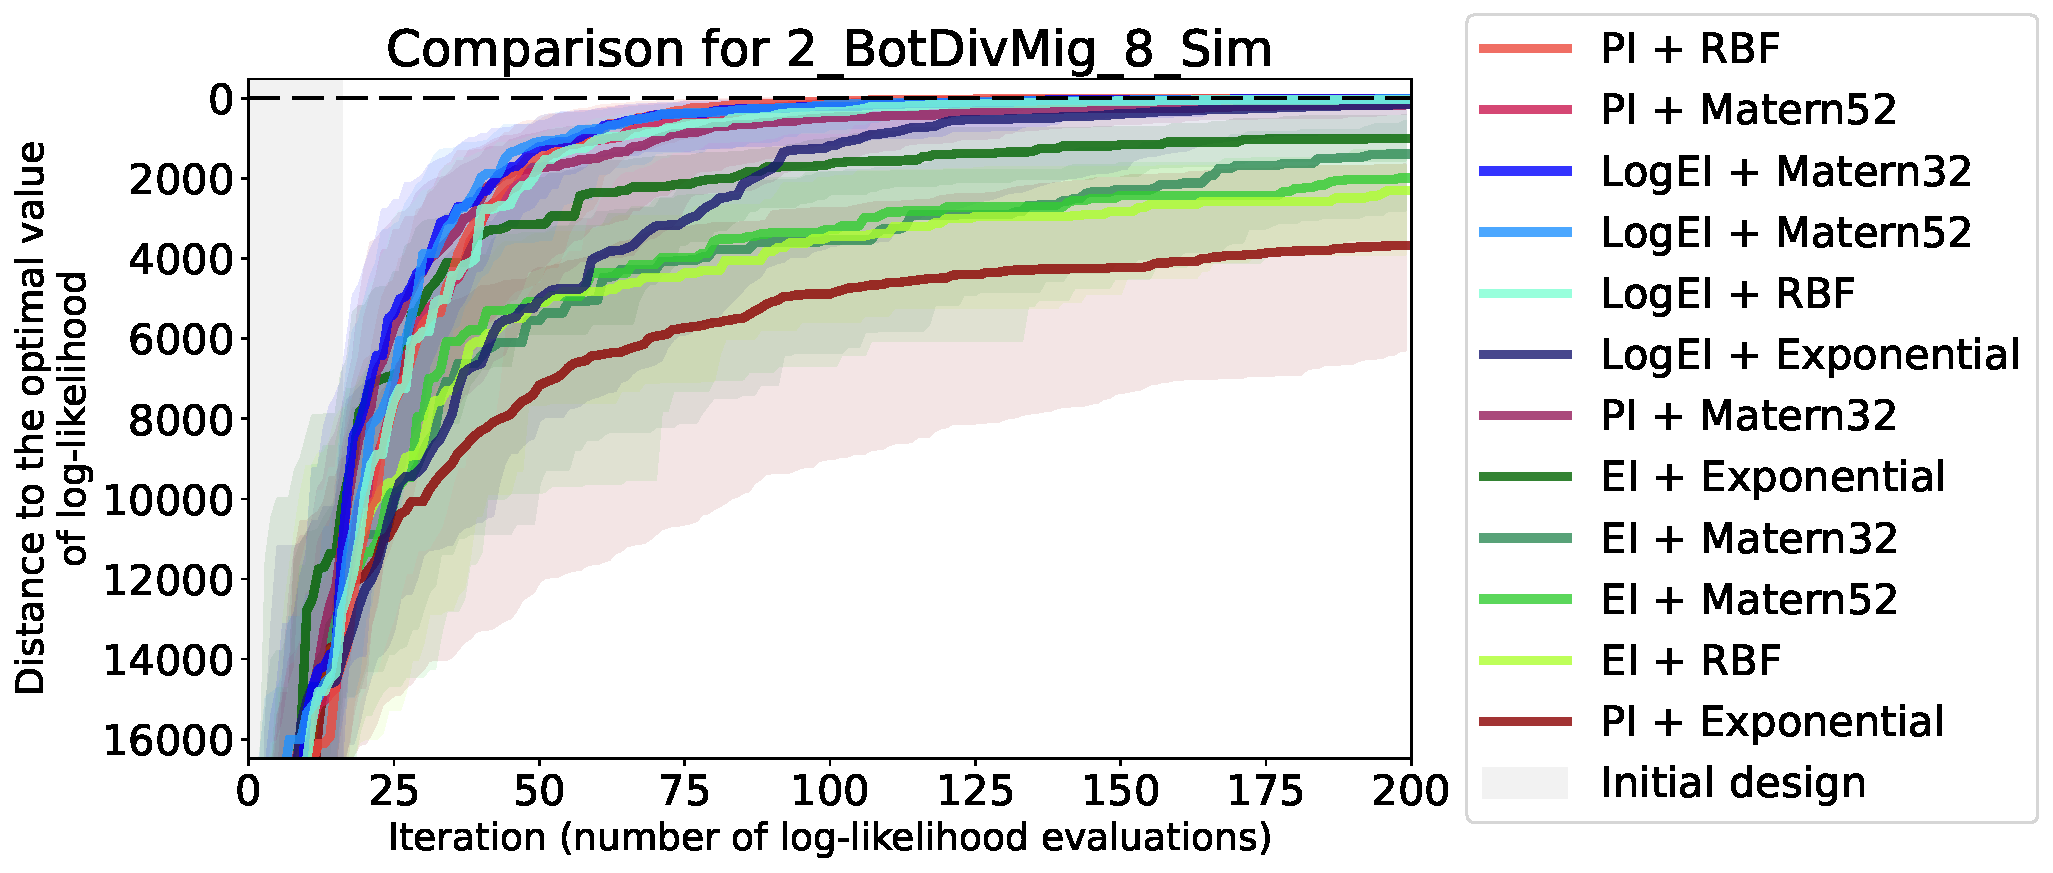
\includegraphics[height=4.0cm]{images_experiments/bo_hpo/BO_config/2_BotDivMig_8_Sim_bo_conf.pdf}
        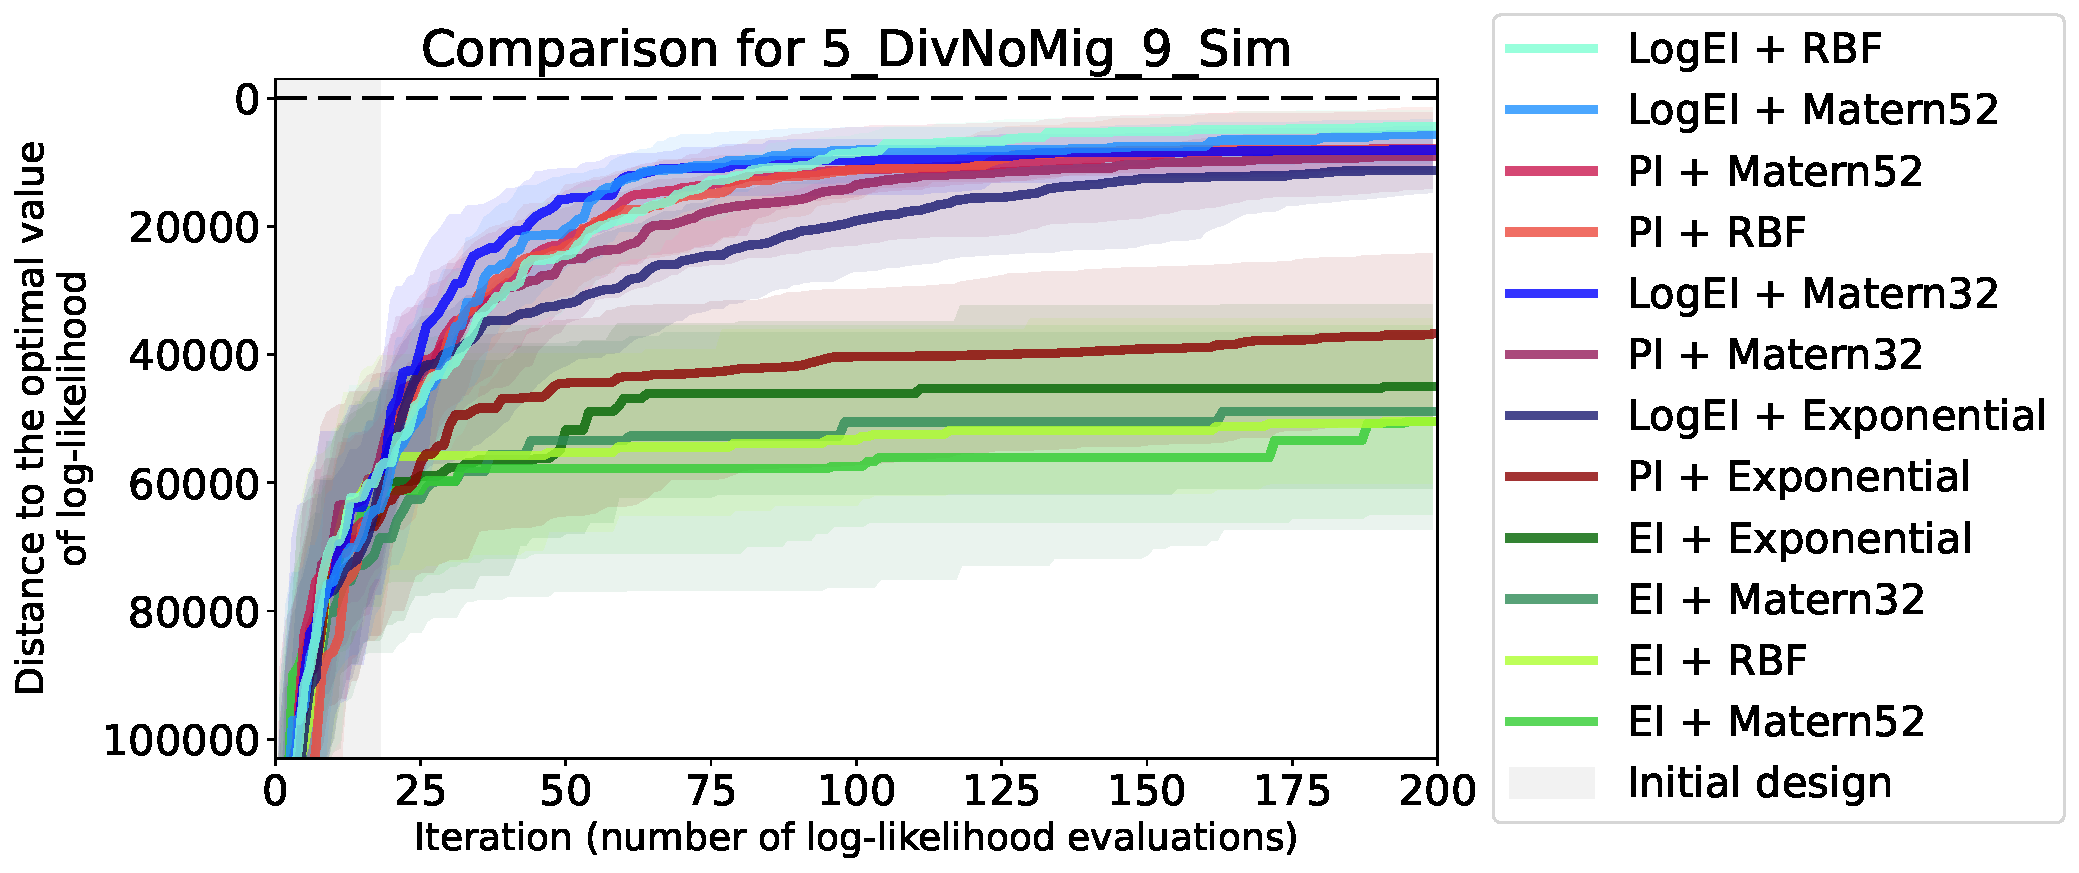
\includegraphics[height=4.0cm]{images_experiments/bo_hpo/BO_config/5_DivNoMig_9_Sim_bo_conf.pdf}
    \caption{Примеры графиков сходимости двенадцати конфигураций классической байесовской оптимизации для датасетов двух и пяти популяций}
    \label{fig:part2:bo_hpo:bo_config}
\end{figure}

Кандидаты конфигураций, которые имеют либо ковариационную функцию \texttt{Exponential}, либо функцию выбора \texttt{EI}, показали худшую сходимость для всех одиннадцати наборов данных.
Ковариационная функция \texttt{Matern52} продемонстрировала лучшую эффективность по сравнению с функцией \texttt{Matern32} в большинстве случаев.
На основе построенных графиков сходимости классической байесовской оптимизации были выделены четыре конфигурации, которые показали наилучшую сходимость.
Они являются комбинацией ковариационных функций \texttt{Matern52} или \texttt{RBF} и функций выбора \texttt{PI} или \texttt{LogEI}:
\begin{itemize}
    \item конфигурация \texttt{Matern52+LogEI};
    \item конфигурация \texttt{Matern52+PI};
    \item конфигурация \texttt{RBF+LogEI};
    \item конфигурация \texttt{RBF+PI}.
\end{itemize}

% \begin{figure}[t]
%     \centering
%     %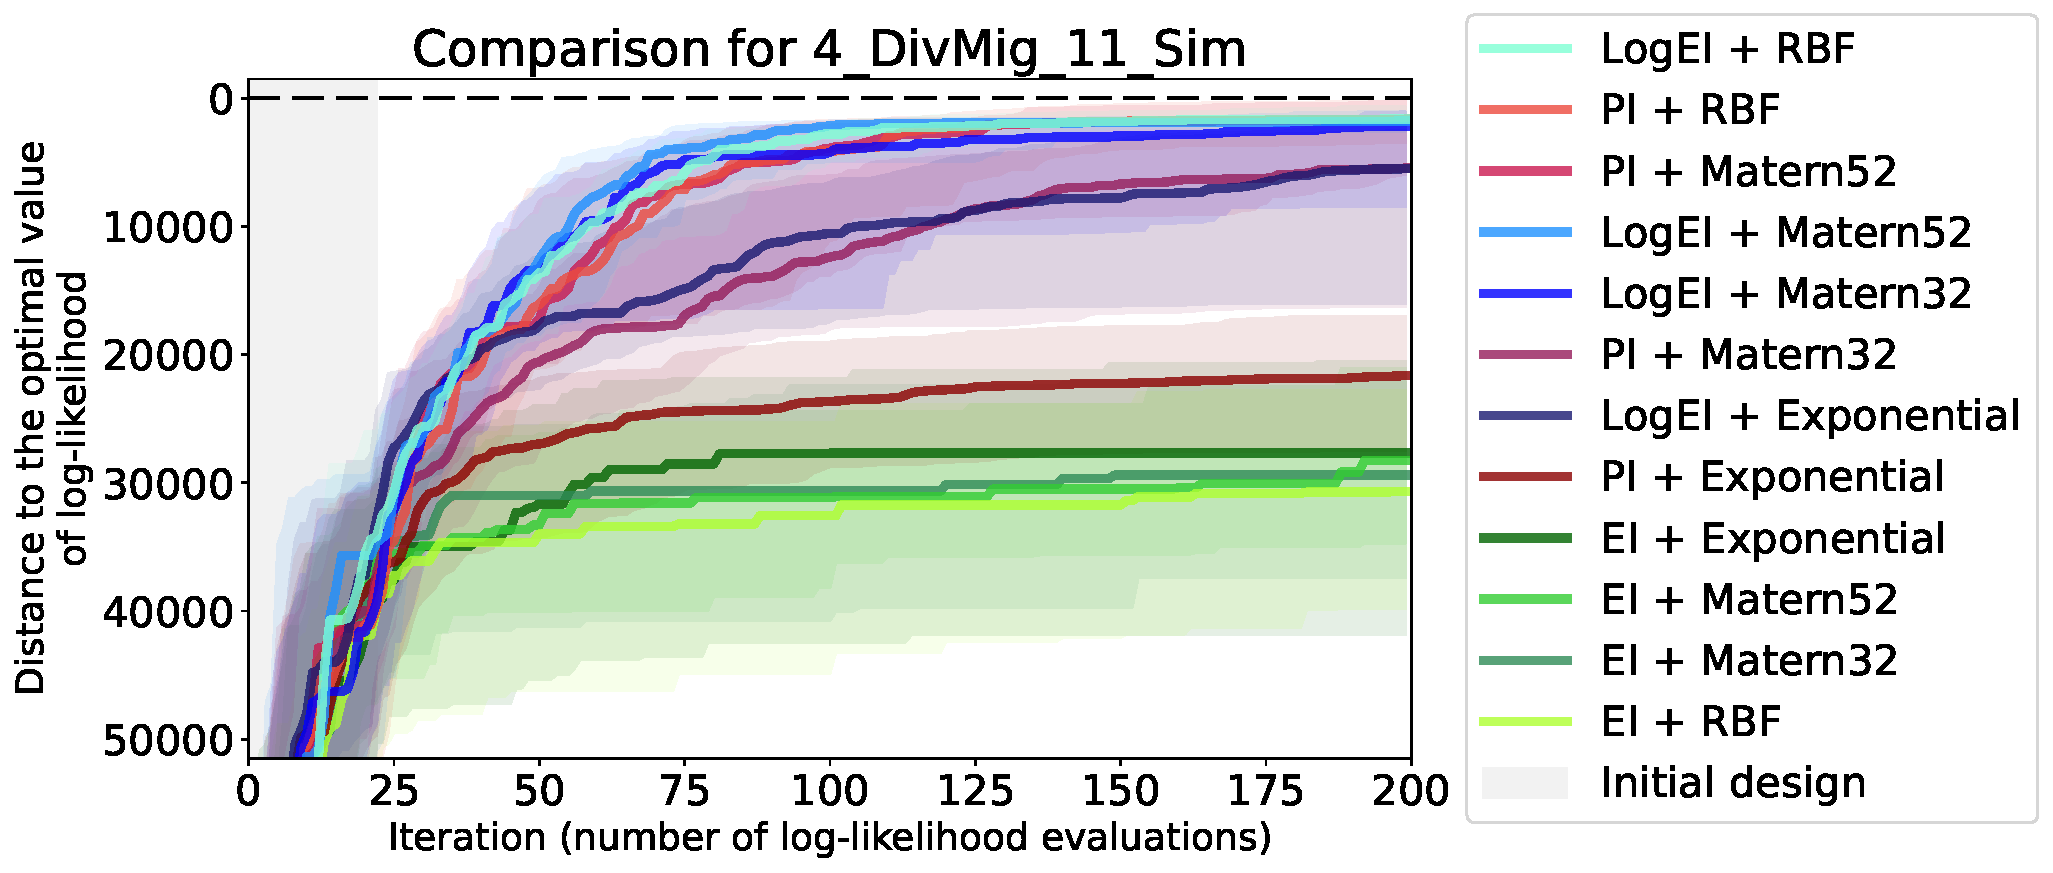
\includegraphics[width=\linewidth]{figures/BO_config/4_DivMig_11_Sim_bo_conf.pdf}
%     \caption{График сходимости $\mathbf{12}$ основных конвейеров байесовской оптимизации для набора данных \texttt{4\_DivMig\_11\_Sim}.
%     Для каждого конвейера-кандидата было независимо выполнено $64$ оптимизационных прогонов. Сплошные линии разных цветов отображают медиану выборки из $64$ значений на каждой итерации, а заштрихованные области - диапазоны между первым и третьим квартилями. Серая область обозначает начальный дизайн, в котором выполняется случайный поиск. Метки в легенде отсортированы в соответствии с итоговой медианой.}
%     \label{fig:bo_conf_conv_plot}
% \end{figure}

Отметим, что результаты полученные по графикам сходимости не согласуются полностью с результатами кросс-валидации.
Заметим, что графики сходимости являются более надежным сравнением, так как они отображают реальную сходимость метода для разных конфигураций на данных.
Например, в случаях, когда метрика $L_{LOO-CV}$ указывает на то, что ковариационная функция \texttt{Exponential} является лучшим выбором, графики сходимости демонстрируют обратное.
Однако оба сравнения сходятся в том, что функция ковариации \texttt{Exponential} является наименее эффективной для решения поставленной задачи.

Далее был разработан и протестирован метод байесовской оптимизации с \emph{автоматическим выбором функции ковариации}.
Перед запуском первой итерации байесовской оптимизации выполняется процедура начального дизайна --- генерации точек случайным образом.
Разработанный метод вычисляет метрику кросс-валидации $L_{LOO-CV}$ на этом наборе начальных точек и выбирает функцию ковариации с наибольшим значением метрики.
Основываясь на результатах экспериментальных исследований двенадцати конфигураций классической байесовской оптимизации, были отобраны две наиболее эффективные функции выбора: \texttt{PI} и \texttt{LogEI}.
Метод байесовской оптимизации с автоматическим выбором функции ковариации был протестирован для каждой из них.
Методы были обозначены, как \texttt{PI+Auto} и \texttt{LogEI+Auto} соответственно.
Было проведено сравнение двух конфигураций между собой, а также с предыдущими лучшими конфигурациями классической байесовской оптимизации.

Для каждого набора данных были построены гистограммы частоты выбора рассматриваемых функций ковариации (рисунок~\ref{fig:part2:bo_hpo:kernel_sel_hists}).
Согласно гистограммам, частота выбора функций различается в зависимости от набора данных, однако \texttt{RBF} и \texttt{Matern52} выбираются наиболее часто.

\begin{figure}[ht]
    \centering
    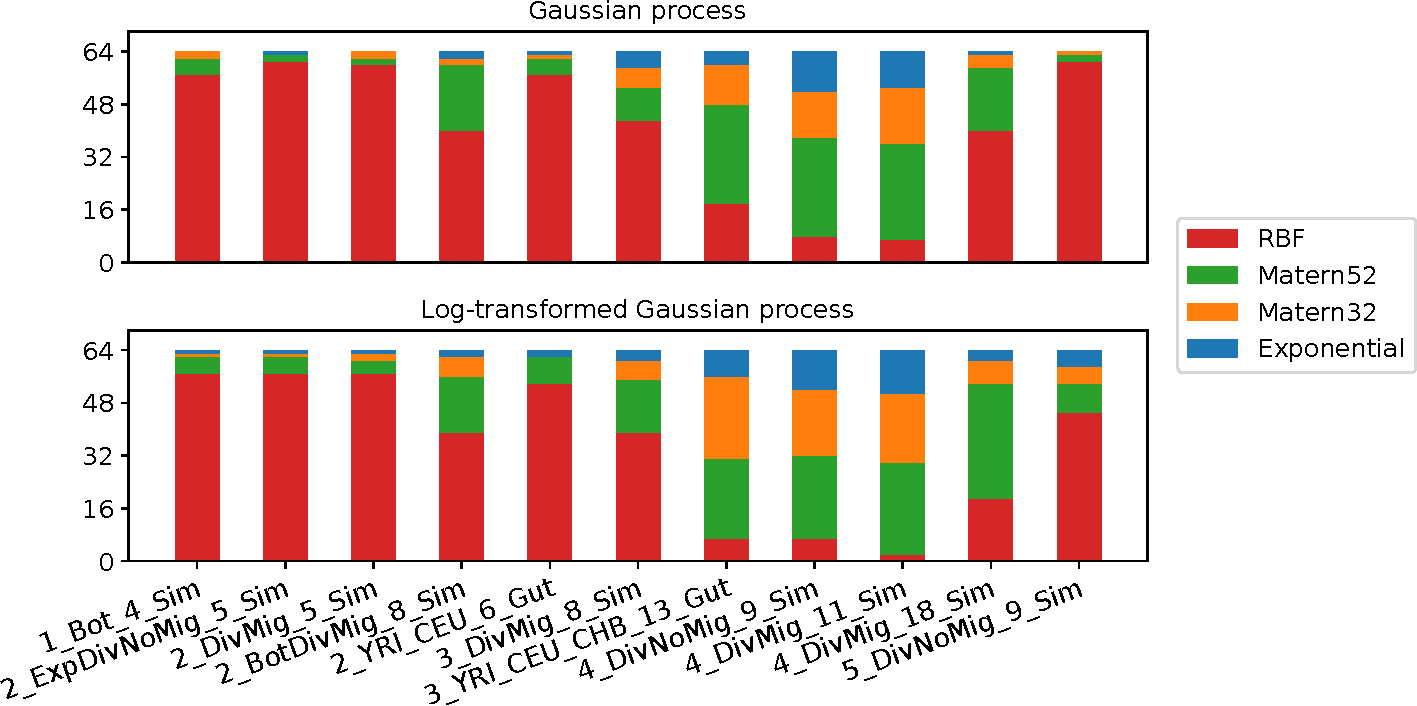
\includegraphics[width=\linewidth]{images_experiments/bo_hpo/kernel_selection_hists.pdf}
    \caption{Гистограммы частоты выбора функций ковариации при применении баесовской оптимизации с автоматическим выбором функции ковариации}
    \label{fig:part2:bo_hpo:kernel_sel_hists}
\end{figure}

Были построены графики сходимости для первых 200 итераций для конфигураций \texttt{PI+Auto} и \texttt{LogEI+Auto} метода с автоматическим выбором функции ковариации.
Эти графики представлены на рисунках~S4~--~S6 в работе~\cite{noskova2023bayesian}.
Два примера графиков представлены на рисунке~\ref{fig:part2:bo_hpo:bo_auto}.
Полученные результаты демонстрируют, что конфигурации имеют равную или лучшую сходимость по сравнению с наилучшими конфигурациями классической байесовской оптимизации.
Однако, определение однозначного победителя среди \texttt{PI+Auto} и \texttt{LogEI+Auto} представляет сложность.
Например, для трех наборов данных --- \texttt{3\_DivMig\_8\_Sim}, \texttt{4\_DivNoMig\_9\_Sim} и \texttt{4\_DivMig\_11\_Sim} --- метод \texttt{LogEI+Auto} показывает лучшую производительность по сравнению с методом \texttt{PI+Auto}.
Для двух наборов данных --- \texttt{3\_YRI\_CEU\_CHB\_13\_Gut} и \texttt{5\_DivNoMig\_9\_Sim} --- результаты оказываются противоположными.
Таким образом, невозможно однозначно определить превосходство какой-либо функции выбора для метода байесовской оптимизации с автоматическим выбором функции ковариации.

\begin{figure}
    \centering
        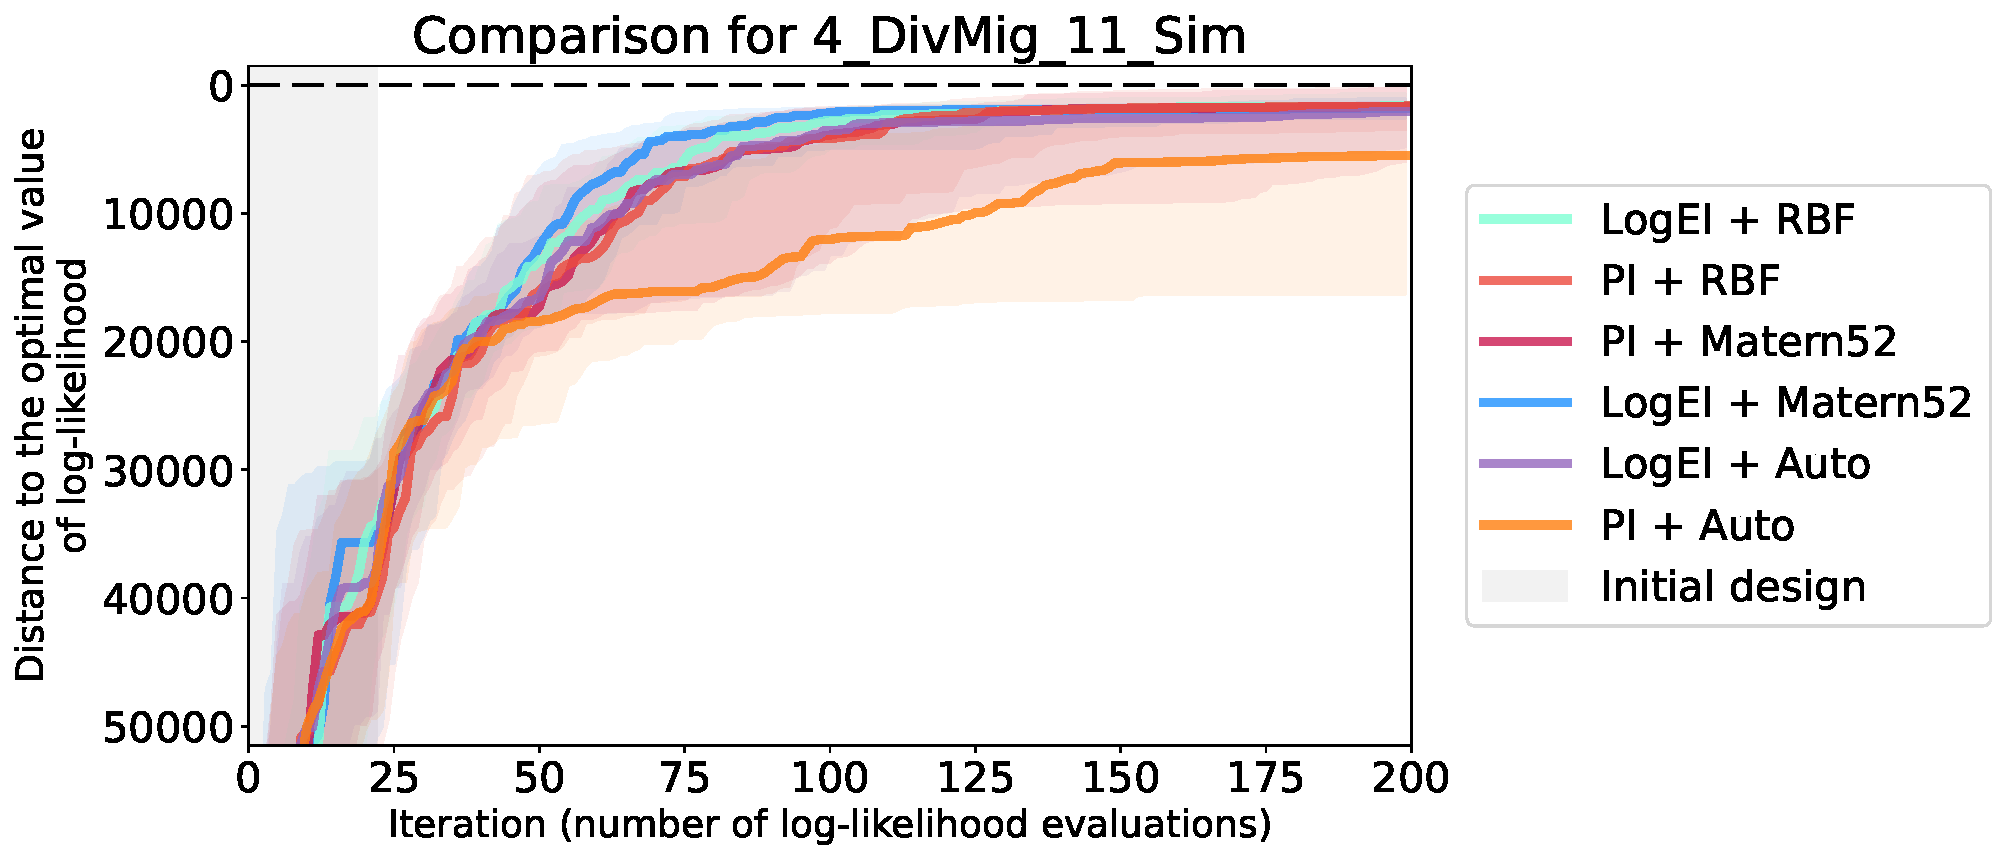
\includegraphics[height=4.0cm]{images_experiments/bo_hpo/BO_auto/4_DivMig_11_Sim_bo_auto.pdf}
        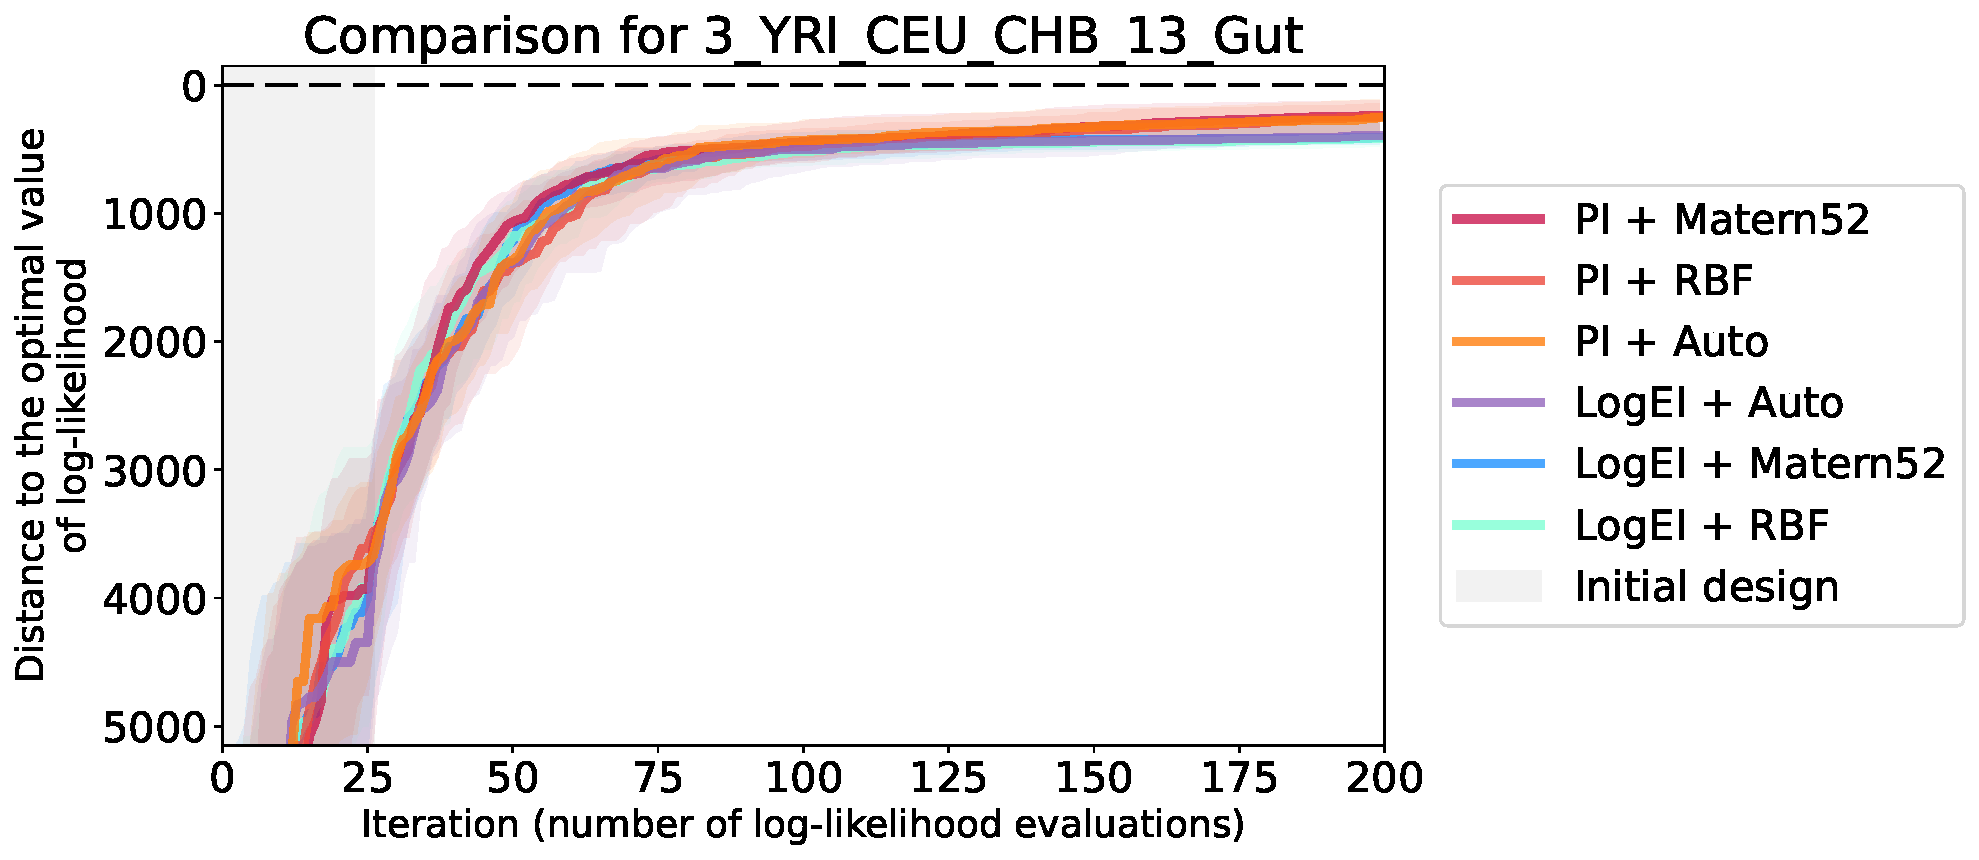
\includegraphics[height=4.0cm]{images_experiments/bo_hpo/BO_auto/3_YRI_CEU_CHB_13_Gut_bo_auto.pdf}
    \caption{Примеры графиков сходимости двух конфигураций байесовской оптимизации с автоматическим выбором функции ковариации и четырех наилучших конфигураций классической байесовской оптимизации для наборов данных трех и четырех популяций}
    \label{fig:part2:bo_hpo:bo_auto}
\end{figure}

Комбинирование подходов и разработка ансамблевых методов является перспективным направлением при решении задач оптимизации.
Совместное использование нескольких методов может привести к значительно более эффективным результатам.
Например, ансамблевый метод байесовской оптимизации под названием Squirrel~\cite{awad2020squirrel} стал одним из победителей конкурса \emph{Black-box Optimization Challenge} в 2020 году.

Основываясь на этих идеях, был разработан ансамблевый метод \texttt{Ensemble} байесовской оптимизации для настройки параметров моделей демографической истории по генетическим данным.
Он представляет собой байесовскую оптимизацию с автоматическим выбором функции ковариации и с ансамблем из двух функций выбора (\texttt{PI} и \texttt{LogEI}).
На каждой итерации равновероятно выбирается одна из функций \texttt{PI} и \texttt{LogEI}, и выполняется поиск новой точки для вычисления целевой функции.
Набор функций ковариации для автоматического выбора был ограничен двумя наиболее эффективными и часто выбираемыми: \texttt{RBF} и \texttt{Matern52}.
Заметим, что функции ковариации для рассматриваемых функций выбора определяются разными способами: для \texttt{PI} регрессия гауссовского процесса строится для целевой функции $f^{moments}$ в то время, как для \texttt{LogEI} регрессия использует логарифмированные значения~$\log f^{moments}(\theta)$.

Были построены графики сходимости метода \texttt{Ensemble} и было выполнено сравнение с двумя наилучшими конфигурациями \texttt{PI+Auto} и \texttt{LogEI+Auto}.
Полученные графики приведены в~\cite{noskova2023bayesian} на рисунках S7~--~S9.
Два примера графиков представлены на рисунке~\ref{fig:part2:bo_hpo:bo_ens}.
Они демонстрируют, что разработанный метод \texttt{Ensemble} имеет наилучшую сходимость среди рассмотренных методов на всех наборах данных.
Метод \texttt{Ensemble} был выбран в качестве финального метода байесовской оптимизации для настройки параметров моделей демографической истории.
На некоторых наборах данных он показал значительные улучшения в сходимости по сравнению с другими байесовскими оптимизациями, например, на \texttt{4\_DivNoMig\_9\_Sim} (рисунок~\ref{fig:part2:bo_hpo:bo_ens}) и на \texttt{4\_DivMig\_11\_Sim}.

\begin{figure}
    \centering
        \includegraphics[height=4.0cm]{images_experiments/bo_hpo/BO_Ens/4_DivNoMig_9_Sim_comp.pdf}
        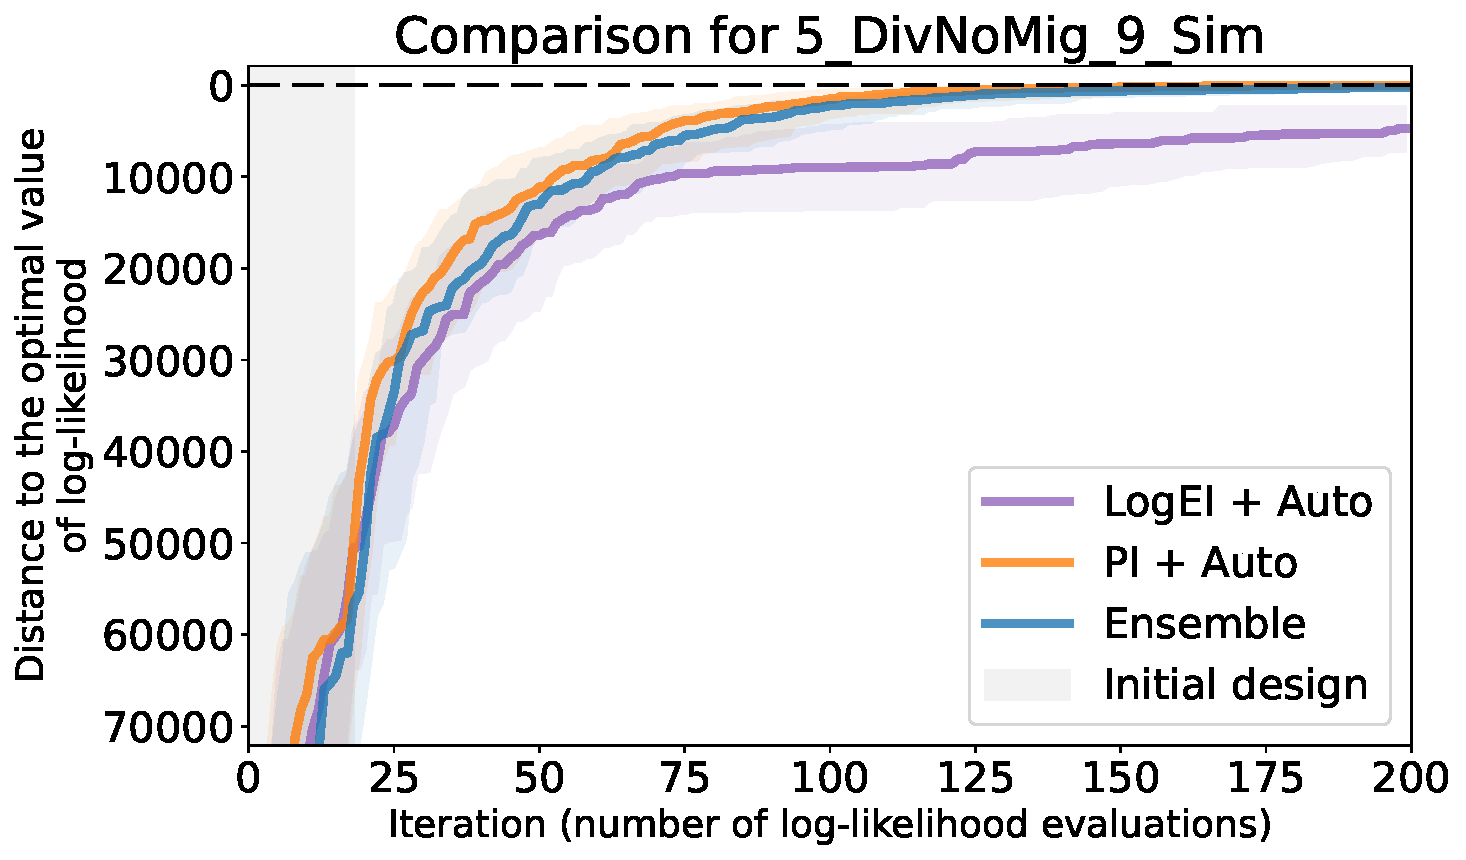
\includegraphics[height=4.0cm]{images_experiments/bo_hpo/BO_Ens/5_DivNoMig_9_Sim_comp.pdf}
    \caption{Примеры графиков сходимости ансамблевого метода байесовской оптимизации и двух конфигураций метода с автоматическим выбором функции ковариации для наборов данных четырех и пяти популяций}
    \label{fig:part2:bo_hpo:bo_ens}
\end{figure}


% \begin{figure}[b!]
%     \centering
%     %\includegraphics[width=0.8\linewidth]{figures/BO_Ens/4_DivNoMig_9_Sim_comp.pdf}
%     \caption{Графики сходимости ранее рассмотренных лучших исполнителей и нового ансамблевого подхода на наборе данных \texttt{4\_DivNoMig\_9\_Sim}, показывающие превосходство последнего.
%     Значение цветных сплошных линий, заштрихованных областей и серой области слева такое же, как на рисунке~\ref{fig:bo_conf_conv_plot}.}
%     \label{fig:bo_auto_conv_plot}
% \end{figure}


\section{Экспериментальные исследования разработанного метода настройки параметров моделей, основанного на комбинации генетического алгоритма и локального поиска для данных одной, двух и трех популяций}
\label{sec:part2:experiments:genetic_algorithm}

Были проведены экспериментальные исследования для определения эффективности разработанного метода для настройки параметров моделей демографической истории по генетическим данным (раздел~\ref{sec:part2:genenic_algorithm}), который основан на комбинации генетического алгоритма и локального поиска.
Разработанный метод был сравнен с существующими методами настройки параметров моделей первого класса, основанных на методах локальной оптимизации, на симулированных и реальных данных одной, двух и трех популяций.
Также метод был применен для настройки параметров моделей расширенного класса, которые включают дискретные параметры динамики изменения численности.
Результаты настройки параметров различных моделей, включая расширенные, с использованием набора существующих методов вычисления правдоподобия были получены автором, а их сравнение приведено ниже.
Для реальных данных, которые ранее были проанализированы в других исследованиях, были получены демографические истории с лучшим значением правдоподобия и информационного критерия Акаике, чем было получено ранее.
В данном разделе приведены результаты этих экспериментальных исследований.


\subsection{Сравнение с существующими методами настройки параметров на симулированных данных одной, двух и трех популяций}
\label{sec:part2:experiments:genetic_algorithm:simulated_data}

Были проведены экспериментальные исследования на симулированных данных для демонстрации расширенного класса моделей и для выявления эффективности метода настройки параметров, основанного на комбинации генетического алгоритма и локального поиска.
Три набора данных были симулированы с использованием следующих демографических историй:

\begin{enumerate}
    \item История «бутылочного горлышка» для одной популяции,
    \item Разделение предковой популяции с асимметричной миграцией между двумя популяциями-потомками,
    \item Вторичный контакт с симметричной миграцией для трех популяций после разделения одной из двух популяций-потомков.
\end{enumerate}

Для каждой истории были симулированы данные в виде аллель-частотных спектров с использованием \moments.
Каждый аллель-частотный спектр имел размер в 20 гаплоидных хромосом на популяцию.
Длина последовательности равна $10^8$ пар оснований, вероятность мутации равна $1{,}25\cdot10^{-8}$ на одну позицию генома на одно поколение.

Для каждого набора данных были сравнены три метода настройки параметров: 1) метод Пауэлла с перезапусками, доступный в \moments, 2) \textit{moments-pipeline}, который реализует набор раундов метода Нелдера-Мида с последовательными запусками, 3) GA+P --- разработанный метод на основе комбинации генетического алгоритма и локального поиска --- метода Пауэлла.
Число перезапусков в первом методе Пауэлла и число раундов для второго метода \textit{\dadi pipeline} были выбраны таким образом, чтобы среднее число вычислений целевой функции совпадало со средним значением, полученным для GA+P.
Например, в случае одной популяции для метода Пауэлла было использовано 40 перезапусков, а для \textit{moments-pipeline} были использованы пять раундов.
Первые четыре раунда включали по 10 запусков метода Нелдера-Мида в каждом, последний пятый раунд включал 20 запусков.

Каждый метод был повторен 50 раз для одной и двух популяций и 10 раз для трех популяций.
Для каждого метода были записаны среднее время одного запуска, среднее число вычислений целевой функции, среднее и стандартное отклонение финального логарифма правдоподобия и наилучшее значение логарифма правдоподобия среди повторов.
Было также зарегистрировано среднее время одного запуска каждой оптимизации, однако оно представлено только в информационных целях.
Вычислительные ресурсы разных методов следует сравнивать, используя число вычислений целевой функции, так как ни у одного метода нет накладных расходов --- вычисления целевой функции занимают почти все время работы метода, а время вычисления правдоподобия может сильно варьироваться в зависимости от значений параметров.

В случае каждого набора симулированных данных вывод демографической истории был проведен для двух моделей.
Первая модель --- модель первого класса с непрерывными параметрами, которая способна воспроизвести историю, используемую в симуляции.
Для этой модели было выполнено сравнение всех трех методов настройки параметров.
Вторая использованная модель --- новая расширенная модель, которая не только способна восстановить первоначальную историю, но и дополнительно имеет дискретные параметры динамики изменения численности.
Для настройки параметров второй модели использовался исключительно метод~GA+P.

Для одной популяции была выбрана демографическая история «бутылочное горлышко»: эффективный размер предковой популяции составлял $10{\,}000$ особей, затем $1{\,}100$ поколений назад произошло «бутылочное горлышко» --- размер популяции составлял 100 особей в течение 100 поколений, после чего численность популяции снова увеличилась до $10{\,}000$ особей.
Рисунок~\ref{fig:part2:experiments:simulated_1:data} демонстрирует описанную демографическую историю (рисунок~\ref{fig:part2:experiments:simulated_1:data_1}), а также симулированные генетические данные в виде аллель-частотного спектра (рисунок~\ref{fig:part2:experiments:simulated_1:data_2}).
Истинная демографическая история имеет серый цвет, чтобы отобразить тот факт, что она использовалась в симуляции.

\begin{figure}[ht]
    \centering
    \begin{subfigure}[b]{.33\textwidth}
    \includegraphics[width=\textwidth]{images_experiments/simulation_1/1pop/picture_1pop_ground_truth_grey.pdf}
    \caption{}
    \label{fig:part2:experiments:simulated_1:data_1}
    \end{subfigure}%
    \begin{subfigure}[b]{.5\textwidth}
    \includegraphics[width=\textwidth]{images_experiments/simulation_1/1pop/1d_plot.pdf}
    \caption{}
    \label{fig:part2:experiments:simulated_1:data_2}
    \end{subfigure}
    \caption{Демографическая история одной популяции, которая была использована для симуляции данных и симулированные генетические данные в виде аллель-частотного спектра}
    \label{fig:part2:experiments:simulated_1:data}
\end{figure}

Две модели, представленные на рисунке~\ref{fig:part2:experiments:simulated_1:models}, были использованы для симулированных данных одной популяции: 1) модель 1 из первого класса моделей с пятью непрерывными параметрами (рисунок~\ref{fig:part2:experiments:simulated_1:models_1}), 2) модель 2 из расширенного класса моделей с пятью непрерывными параметрами и двумя дискретными параметрами динамики (рисунок~\ref{fig:part2:experiments:simulated_1:models_2}).

\begin{figure}[ht]
    \centering
    \begin{subfigure}[b]{.33\textwidth}
    \includegraphics[width=\textwidth]{images_experiments/simulation_1/1pop/picture_1pop_model_1.pdf}
    \caption{}
    \label{fig:part2:experiments:simulated_1:models_1}
    \end{subfigure}%
    \begin{subfigure}[b]{.33\textwidth}
    \includegraphics[width=\textwidth]{images_experiments/simulation_1/1pop/picture_1pop_model_2.pdf}
    \caption{}
    \label{fig:part2:experiments:simulated_1:models_2}
    \end{subfigure}
    \caption{Используемые модели для сравнения методов на симулированных данных одной популяции}
    \label{fig:part2:experiments:simulated_1:models}
\end{figure}

Для каждого повтора метод Пауэлла был запущен 40 раз, а \textit{moments-pipeline} состоял из пяти раундов: первые четыре раунда включали по 10 запусков метода Нелдера-Мида в каждом, последний пятый раунд состоял из 20 запусков.
Результаты представлены в таблице~\ref{tab:part2:experiments:simulated_1:results}. Изображения полученных демографических историй для модели 1 показаны на рисунке~\ref{fig:part2:experiments:simulated_1:results_model_1}: а) метод Пауэлла с перезапусками, б) метод \textit{moments-pipeline}, в) метод GA+P.
На рисунке~\ref{fig:part2:experiments:simulated_1:results_model_2} приведены две альтернативные демографические истории для модели 2, полученные методом GA+P.
Все истории, изображенные на рисунках~\ref{fig:part2:experiments:simulated_1:results_model_1}~и~\ref{fig:part2:experiments:simulated_1:results_model_2}, наложены на истинную демографическую историю, использованную в симуляциях, для демонстрации разницы.

\begin{table}[ht]
    \caption{Результаты 50 повторов тестируемых методов настройки параметров для моделей демографической истории одной популяции}
    \resizebox{\linewidth}{!}{
    \begin{tabular}{|l|c| c c c| c c|}
    \hline
  &  & \multicolumn{3}{c|}{Модель 1} & \multicolumn{2}{c|}{Модель 2}\\ 
  \hline
 & Истинные & Метод Пауэлла  & \multirow{2}{*}{\textit{moments-pipeline}} & \multirow{2}{*}{GA+P}  & \multicolumn{2}{c|}{GA+P}\\
 & значения & с перезапусками & & & Вариант 1 & Вариант 2\\ 
 \hline
  Среднее время & $-$ & $06^\text{мин}40^\text{сек}$  & $05^\text{мин}22^\text{сек}$ & $07^\text{мин}25^\text{сек}$ & \multicolumn{2}{c|}{$12^\text{мин}54^\text{сек}$}\\
 Среднее число & \multirow{2}{*}{$-$} & \multirow{2}{*}{$7{\,}860$} & \multirow{2}{*}{$7{\,}951$} & \multirow{2}{*}{$7{\,}515$} & \multicolumn{2}{c|}{\multirow{2}{*}{$13{\,}688$}}\\
 итераций & & & & & &\\
 Среднее $f^{moments}$ & $ - $ & $-293{,}4815$ & $-338{,}1879$ & $-132{,}9586$ &  \multicolumn{2}{c|}{$-97{,}9999$}
\\
 Ст. откл. $f^{moments}$ & $ - $ & $136{,}2765$ & $116{,}9429$ & $99{,}9209$ &  \multicolumn{2}{c|}{$43{,}5008$}\\
 \hline
 Лучшее $f^{moments}$ & $-88{,}5603$ & $-88{,}6202$ & $-88{,}5780$ & $-88{,}5832$ & $\mathbf{-88{,}5616}$ & $-88{,}5711$\\
    \hline 
    $N_A$ & 10000 & 9999 & 10028 & 10038 & 10034 & 10018 \\
    $N_B$ & 100 & 219 & 203 & 201 &  178$^e$ & 180\\
    $N_F$ & 10000 & 10180 & 10159 & 10094 &  10050 & 10011 \\
    $T_B$ & 100 & 112 & 103 & 205 & 791 & 182\\
    $T$ & 1000 & 971 & 975 & 978& 985 & 986\\
    \hline
    \end{tabular}}
    \label{tab:part2:experiments:simulated_1:results}
\end{table}

\begin{figure}[ht]
    \centering
    \begin{subfigure}[b]{.33\textwidth}
    \includegraphics[width=\textwidth]{images_experiments/simulation_1/1pop/picture_1pop_model_1_powell_over.pdf}
    \caption{}
    \label{fig:part2:experiments:simulated_1:results_model_1_1}
    \end{subfigure}%
    \begin{subfigure}[b]{.33\textwidth}
    \includegraphics[width=\textwidth]{images_experiments/simulation_1/1pop/picture_1pop_model_1_dadi_pipeline_over.pdf}
    \caption{}
    \label{fig:part2:experiments:simulated_1:results_model_1_2}
    \end{subfigure}%
    \begin{subfigure}[b]{.33\textwidth}
    \includegraphics[width=\textwidth]{images_experiments/simulation_1/1pop/picture_1pop_model_1_ga_over.pdf}
    \caption{}
    \label{fig:part2:experiments:simulated_1:results_model_1_3}
    \end{subfigure}
    \caption{Демографические истории, полученные путем настройки параметров модели 1 разными методами}
    \label{fig:part2:experiments:simulated_1:results_model_1}
\end{figure}

\begin{figure}[ht]
    \centering
    \begin{subfigure}[b]{.33\textwidth}
    \includegraphics[width=\textwidth]{images_experiments/simulation_1/1pop/picture_1pop_model_2_ga_1_over.pdf}
    \caption{}
    \label{fig:part2:experiments:simulated_1:results_model_2_1}
    \end{subfigure}%
    \begin{subfigure}[b]{.33\textwidth}
    \includegraphics[width=\textwidth]{images_experiments/simulation_1/1pop/picture_1pop_model_2_ga_2_over.pdf}
    \caption{}
    \label{fig:part2:experiments:simulated_1:results_model_2_2}
    \end{subfigure}
    \caption{Демографические истории, полученные путем настройки параметров модели 2 методом GA+P}
    \label{fig:part2:experiments:simulated_1:results_model_2}
\end{figure}

Для модели 1 метод GA+P показал лучшее среднее и стандартное отклонение логарифма правдоподобия, однако метод \textit{moments-pipeline} показал лучшее значение максимального правдоподобия среди трех оптимизаций.
Для модели 2 метод GA+P показал наилучшие среднее и стандартное отклонение логарифма вероятности по 50 повторам, а также предоставил две альтернативные истории со схожими значениями правдоподобия.
Первая из них --- вариант 1 включает экспоненциальное уменьшение численности популяции и внезапный рост после, а вторая --- вариант 2 имеет постоянные динамики численности популяции и похожа на истинную историю.
Данный результат является следствием того, что одному аллель-частотному спектру может соответствовать несколько демографических историй.
Похожие демографические истории были представлены в~\cite{myers2008can}, как пример историй, которые имеют одинаковые ожидаемые спектры. 



Для двух популяций была выбрана следующая демографическая история: эффективный размер предковой популяции составлял $10{\,}000$, $1{\,}000$ поколений назад она разделилась на две популяции с размерами $10{\,}000$ особей (Популяция 1) и $1{\,}000$ особей (Популяция 2).
Непрерывная миграция между популяциями равна: $2{,}5 \times 10^{-4}$ особей из популяции 2 в популяцию 1 за поколение и $1{,}25 \times 10^{-4}$ особей из популяции 1 в популяцию 2 за поколение.
Рисунок~\ref{fig:part2:experiments:simulated_2:data} демонстрирует описанную демографическую историю (рисунок~\ref{fig:part2:experiments:simulated_2:data_1}), а также симулированные генетические данные в виде аллель-частотного спектра (рисунок~\ref{fig:part2:experiments:simulated_2:data_2}).
Метод Пауэлла имел шесть перезапусков, а метод \textit{moments-pipeline} был запущен для четырех раундов первые три раунда включали по 10 запусков метода Нелдера-Мида в каждом, последний четвертый раунд состоял из 20 запусков.
Две использованные модели изображены на рисунке~\ref{fig:part2:experiments:simulated_2:models}.

\begin{figure}[ht]
    \centering
    \begin{subfigure}[b]{.4\textwidth}
    \includegraphics[width=\textwidth]{images_experiments/simulation_1/2pop/picture_1pop_ground_truth_grey.pdf}
    \caption{}
    \label{fig:part2:experiments:simulated_2:data_1}
    \end{subfigure}%
    \begin{subfigure}[b]{.4\textwidth}
    \includegraphics[width=\textwidth]{images_experiments/simulation_1/2pop/2d_plot.pdf}
    \caption{}
    \label{fig:part2:experiments:simulated_2:data_2}
    \end{subfigure}
    \caption{Демографическая история двух популяции, которая была использована для симуляции данных и симулированные генетические данные в виде аллель-частотного спектра}
    \label{fig:part2:experiments:simulated_2:data}
\end{figure}

\begin{figure}[ht]
    \centering
    \begin{subfigure}[b]{.4\textwidth}
    \includegraphics[width=\textwidth]{images_experiments/simulation_1/2pop/picture_1pop_model_1.pdf}
    \caption{}
    \label{fig:part2:experiments:simulated_2:models_1}
    \end{subfigure}%
    \begin{subfigure}[b]{.4\textwidth}
    \includegraphics[width=\textwidth]{images_experiments/simulation_1/2pop/picture_1pop_model_2.pdf}
    \caption{}
    \label{fig:part2:experiments:simulated_2:models_2}
    \end{subfigure}
    \caption{Используемые модели для сравнения методов на симулированных данных двух популяций}
    \label{fig:part2:experiments:simulated_2:models}
\end{figure}



Результаты представлены в таблице~\ref{tab:part2:experiments:simulated_2:results}. Изображения полученных демографических историй для модели 1 показаны на рисунке~\ref{fig:part2:experiments:simulated_2:results_model_1}: а) метод Пауэлла с перезапусками, б) метод \textit{moments-pipeline}, в) метод GA+P.
На рисунке~\ref{fig:part2:experiments:simulated_2:results_model_2} приведена демографическая история для модели 2, полученная методом GA+P.
Все истории, изображенные на рисунках~\ref{fig:part2:experiments:simulated_2:results_model_1}~и~\ref{fig:part2:experiments:simulated_2:results_model_2}, наложены на истинную демографическую историю, использованную в симуляциях, для демонстрации разницы.

\begin{table}[ht!]
    \caption{Результаты 50 повторов тестируемых методов настройки параметров для моделей демографической истории двух популяций}
    \resizebox{\linewidth}{!}{
    \begin{tabular}{|l | c | c c c | c|}
    \hline
    &  & \multicolumn{3}{c|}{Модель 1} & Модель 2\\ 
    \hline
    & Истинные & Метод Пауэлла  & \multirow{2}{*}{\textit{moments-pipeline}} & \multirow{2}{*}{GA+P}  & \multirow{2}{*}{GA+P}\\
    & значения & с перезапусками & & & \\ 
    \hline
    Среднее время & $-$ & $30^{\text{мин}}39^{\text{сек}}$ & $55^\text{мин}12^\text{сек}$ & $30^\text{мин}34^\text{сек}$ & $223^\text{мин}24^\text{сек}$\\
    Среднее число & \multirow{2}{*}{$-$} & \multirow{2}{*}{$7626$} & \multirow{2}{*}{$8928$} & \multirow{2}{*}{$7437$} & \multirow{2}{*}{$17136$}\\
    итераций & & & & & \\
    Среднее $f^{moments}$: & $-$ & $-1310{,}948$ & $-1311{,}016$ & $-1311{,}269$ & $-1321{,}195$\\
    Ст. откл. $f^{moments}$ & $ - $ & $0{,}027$ & $0{,}241$ & $0{,}451$ & $13{,}861$\\
    \hline
    Лучшее $f^{moments}$ & $-1310{,}931$ & $\mathbf{1310{,}931}$ & $-1310{,}932$ & $\mathbf{-1310{,}931}$ &  $-1310{,}983$\\
    \hline
    $N_A$ & 10000 & 10000 & 10001 & 10000 & 10001\\
    $N_1$ & 10000 & 10000 & 9992 & 10003 & 10007\\
    $N_2$ & 1000 & 1000 & 1000 & 1000 & 997\\
    $m_{12} (\times 10^{-4})$ & 2.50 & 2.50 & 2.50 & 2.50 & 2.50 \\
    $m_{21} (\times 10^{-4})$ & 1.25 & 1.25 & 1.25 & 1.25 & 1.26\\
    $T$ & 1000 & 1000 & 1000 & 1000 & 996\\
    \hline
    \end{tabular}%
    }
    \label{tab:part2:experiments:simulated_2:results}
\end{table}

\begin{figure}[ht]
    \centering
    \begin{subfigure}[b]{.33\textwidth}
    \includegraphics[width=\textwidth]{images_experiments/simulation_1/2pop/picture_1pop_model_1_powell_over.pdf}
    \caption{}
    \label{fig:part2:experiments:simulated_2:results_model_1_1}
    \end{subfigure}%
    \begin{subfigure}[b]{.33\textwidth}
    \includegraphics[width=\textwidth]{images_experiments/simulation_1/2pop/picture_1pop_model_1_dadi_pipeline_over.pdf}
    \caption{}
    \label{fig:part2:experiments:simulated_2:results_model_1_2}
    \end{subfigure}%
    \begin{subfigure}[b]{.33\textwidth}
    \includegraphics[width=\textwidth]{images_experiments/simulation_1/2pop/picture_1pop_model_1_ga_over.pdf}
    \caption{}
    \label{fig:part2:experiments:simulated_2:results_model_1_3}
    \end{subfigure}
    \caption{Демографические истории двух популяций, полученные путем настройки параметров модели 1 разными методами}
    \label{fig:part2:experiments:simulated_2:results_model_1}
\end{figure}

\begin{figure}[ht]
    \centering
    \includegraphics[width=0.33\textwidth]{images_experiments/simulation_1/2pop/picture_1pop_model_2_ga_over.pdf}
    \caption{Демографическая история двух популяций, полученная путем настройки параметров модели 2 методом GA+P}
    \label{fig:part2:experiments:simulated_2:results_model_2}
\end{figure}

Все методы для всех моделей предоставили демографические истории, близкие к истинной, которая была использована для симуляции данных.
Методы Пауэлла и GA+P для модели 1 показали наиболее точные результаты.
Метод Пауэлла в среднем продемонстрировал лучшие результаты, чем метод GA+P.
Метод GA+P корректно восстановил константные динамики изменения численности при настройке параметров модели 2.



Для симуляции данных трех популяций была использована следующая демографическая история.
Эффективный размер предковой популяции составлял $10{\,}000$, затем $3{\,}000$ поколений назад она разделилась на две субпопуляции размером $15{\,}000$ (популяция 1) и $5{\,}000$ (популяция 2 + популяция 3).
Затем вторая субпопуляция разделилась на две новые популяции размером $5{\,}000$ (популяция 2) и $10{\,}000$ (популяция 3).
Непрерывные миграции имели начало только $1{\,}000$ поколений назад сразу после второго разделения и являются симметричными: $0{,}25 \times 10^{-4}$ особей на поколение между популяцией 1 и популяцией 2, $0{,}5 \times 10^{-4}$ между популяцией 1 и популяцией 3 и $1{,}5 \times 10^{-4}$ между популяцией 2 и популяцией 3.
Рисунок~\ref{fig:part2:experiments:simulated_3:data} демонстрирует описанную демографическую историю (рисунок~\ref{fig:part2:experiments:simulated_3:data_1}), а также симулированные генетические данные в виде аллель-частотного спектра (рисунок~\ref{fig:part2:experiments:simulated_3:data_2}).

\begin{figure}[ht]
    \centering
    \begin{subfigure}[b]{.5\textwidth}
    \includegraphics[width=\textwidth]{images_experiments/simulation_1/3pop/picture_1pop_model_ground_truth_grey}
    \caption{}
    \label{fig:part2:experiments:simulated_3:data_1}
    \end{subfigure}%
    \begin{subfigure}[b]{.4\textwidth}
    \includegraphics[width=\textwidth]{images_experiments/simulation_1/3pop/3d_plot.pdf}
    \caption{}
    \label{fig:part2:experiments:simulated_3:data_2}
    \end{subfigure}
    \caption{Демографическая история трех популяции, которая была использована для симуляции данных и симулированные генетические данные в виде аллель-частотного спектра}
    \label{fig:part2:experiments:simulated_3:data}
\end{figure}

Две модели, представленные на рисунке~\ref{fig:part2:experiments:simulated_3:models} были использованы для симулированных данных трех популяции: 1) модель 1 из первого класса моделей с десятью параметрами (рисунок~\ref{fig:part2:experiments:simulated_3:models_1}), 2) модель 2 из расширенного класса моделей с 18 непрерывными параметрами и пятью дискретными параметрами динамики (рисунок~\ref{fig:part2:experiments:simulated_3:models_2}).
Метод Пауэлла имел 12 перезапусков, а метод \textit{moments-pipeline} был запущен для шести раундовЖ первые пять раундов включали по 10 запусков метода Нелдера-Мида в каждом, последний цестой раунд состоял из 20 запусков.

\begin{figure}[ht]
    \centering
    \begin{subfigure}[b]{.5\textwidth}
    \includegraphics[width=\textwidth]{images_experiments/simulation_1/3pop/picture_1pop_model_1.pdf}
    \caption{}
    \label{fig:part2:experiments:simulated_3:models_1}
    \end{subfigure}%
    \begin{subfigure}[b]{.5\textwidth}
    \includegraphics[width=\textwidth]{images_experiments/simulation_1/3pop/picture_1pop_model_2.pdf}
    \caption{}
    \label{fig:part2:experiments:simulated_3:models_2}
    \end{subfigure}
    \caption{Используемые модели для сравнения методов на симулированных данных трех популяций}
    \label{fig:part2:experiments:simulated_3:models}
\end{figure}

Результаты представлены в таблице~\ref{tab:part2:experiments:simulated_3:results}. Изображения полученных демографических историй для модели 1 показаны на рисунке~\ref{fig:part2:experiments:simulated_3:results_model_1}: а) метод Пауэлла с перезапусками, б) метод \textit{moments-pipeline}, в) метод GA+P.
На рисунке~\ref{fig:part2:experiments:simulated_3:results_model_2} приведена демографическая история для модели 2, полученная методом GA+P.
Все истории, изображенные на рисунках~\ref{fig:part2:experiments:simulated_3:results_model_1}~и~\ref{fig:part2:experiments:simulated_3:results_model_2} наложены на истинную демографическую историю, использованную в симуляциях, для демонстрации разницы.

В случае модели 1 для трех популяций метод GA+P продемонстрировал наилучшие значения максимального, среднего и стандартного отклонения значения правдоподобия среди всех наблюдаемых методов.
Настройка параметров модели 2 успешно реконструировала симметричные миграции, а дополнительные параметры оказались близки к истинным значениям.
Однако эта история имеет ненулевую миграцию после раскола предковой популяции, что может быть связано с малым числом повторов.
Все предсказанные динамики, несмотря на то, что не все они являются константными, показывают, что размер популяций оставался почти одинаковым.


\begin{table}[ht!]
    \caption{Результаты 10 повторов тестируемых методов настройки параметров для моделей демографической истории трех популяций}
    \resizebox{\linewidth}{!}{
    \begin{tabular}{|l | c | c c c | c|}
    \hline
    &  & \multicolumn{3}{c|}{Модель 1} & Модель 2\\ 
    \hline
    & Истинные & Метод Пауэлла  & \multirow{2}{*}{\textit{moments-pipeline}} & \multirow{2}{*}{GA+P}  & \multirow{2}{*}{GA+P}\\
    & значения & с перезапусками & & & \\ 
    \hline
    Среднее время & $-$ & $28^\text{ч}28^\text{мин}13^\text{сек}$ & $45^\text{ч}09^\text{мин}30^\text{сек}$ & $27^\text{ч}16^\text{мин}08^\text{сек}$ & $45^\text{ч}05^\text{мин}00^\text{сек}$\\
    Среднее число & \multirow{2}{*}{$-$} & \multirow{2}{*}{$22475$} & \multirow{2}{*}{$19452$} & \multirow{2}{*}{$21651$} & \multirow{2}{*}{$71534$}\\
    вычислений & & & & & \\
    Среднее $f^{moments}$ & $ - $ & $-11178{,}62$ & $-11179{,}82$ & $-11178{,}45$ & $-11250{,}09$\\
    Ст. откл. $f^{moments}$ & $ - $ & $0{,}40$ & $0{,}72$ & $0{,}15$ &  $123{,}72$ \\
    \hline 
    Лучшее $f^{moments}$ & $-11178{,}28$ & $-11178{,}31$ & $-11178{,}59$ & $-11178{,}29$ & $-11180{,}28$\\

    \hline
    $N_A$ & 10000 & 10003 & 9988 & 9996  & 9997\\
    $N_{11}$ & $=N_1$ (15000) & NA & NA & NA & 14612\\
    $N_{23}$ & $=N_2$ (5000) & NA & NA & NA & 4801\\
    $m_{1(23)} (\times 10^{-4})$ & NA (0) & NA & NA & NA & 0.14 \\
    $m^{(23)1} (\times 10^{-4})$ & NA (0) & NA & NA & NA & 0.27\\
    $N_1$ & 15000 & 15018 & 15029 & 15004 & $15567^{exp}$\\
    $N_2$ & 5000 & 4992 & 5011 & 5008 & 5032\\
    $N_3$ & 10000 & 9984 & 9850 & 10026 & 10050\\
    $m_{12} (\times 10^{-4})$ & $0{,}25$ & $0{,}25$ & $0{,}24$ & $0{,}25$ & $0{,}23$\\
    $m_{13} (\times 10^{-4})$ & $0{,}50$ & $0{,}50$ & $0{,}50$ & $0{,}50$ &  $0{,}47$\\
    $m_{21} (\times 10^{-4})$ & $=m_{12}$ ($0{,}25$) & NA & NA & NA & $0{,}21$\\
    $m_{23} (\times 10^{-4})$ & $1{,}50$ & $1{,}51$ & $1{,}55$ & $1{,}50$ &  $1{,}54$\\
    $m_{31} (\times 10^{-4})$ & $=m_{13}$ ($0{,}50$) & NA & NA & NA & $0{,}44$ \\
    $m_{32} (\times 10^{-4})$ & $=m_{23}$ ($1{,}50$) & NA & NA & NA & $1{,}60$ \\
    $T_2$ & 2000 & 1998 & 1996 & 1999 & 2055\\
    $T_1$ & 1000 & 1000 & 1009 & 1000 & 1020\\
    \hline
    \end{tabular}%
    }
    \begin{tablenotes}
      \footnotesize
      \item $^*$ 9/10 повторов. Наихудший повтор имел максимальное значение логарифма правдоподобия, равное~$-13801{,}48$.\\
      \item $^{exp}$ --- экспоненциальное изменение численности.
    \end{tablenotes}
    \label{tab:part2:experiments:simulated_3:results}
\end{table}

\begin{figure}[ht!]
    \centering
    \begin{subfigure}[b]{.33\textwidth}
    \includegraphics[width=\textwidth]{images_experiments/simulation_1/3pop/picture_1pop_model_1_powell_over.pdf}
    \caption{}
    \label{fig:part2:experiments:simulated_3:results_model_1_1}
    \end{subfigure}%
    \begin{subfigure}[b]{.33\textwidth}
    \includegraphics[width=\textwidth]{images_experiments/simulation_1/3pop/picture_1pop_model_1_dadi_pipeline_over.pdf}
    \caption{}
    \label{fig:part2:experiments:simulated_3:results_model_1_2}
    \end{subfigure}%
    \begin{subfigure}[b]{.33\textwidth}
    \includegraphics[width=\textwidth]{images_experiments/simulation_1/3pop/picture_1pop_model_1_ga_over.pdf}
    \caption{}
    \label{fig:part2:experiments:simulated_3:results_model_1_3}
    \end{subfigure}
    \caption{Демографические истории трех популяций, полученные путем настройки параметров модели 1 разными методами}
    \label{fig:part2:experiments:simulated_3:results_model_1}
\end{figure}

\FloatBarrier
\clearpage
\begin{figure}[t!]
    \centering
    \includegraphics[width=0.33\textwidth]{images_experiments/simulation_1/3pop/picture_1pop_model_2_ga_over.pdf}
    \caption{Демографическая история трех популяций, полученная путем настройки параметров модели 2 методом GA+P}
    \label{fig:part2:experiments:simulated_3:results_model_2}
\end{figure}


\subsection{Сравнение с существующими методами настройки параметров моделей на данных популяций кошачьей лягушки}
\label{part2:frogs}

Разработанный метод, основанный на комбинации генетического алгоритма и локального поиска, был сравнен с методом множественного запуска метода Нелдера-Мида, реализованным в программном средстве \textit{dadi-pipeline}~\cite{portik2017evaluating}.
В статье~\cite{portik2017evaluating}, в которой был впервые представлен \textit{dadi-pipeline}, его эффективность была продемонстрирована на данных для кошачьей лягушки (\textit{Scotobleps gabonicus}).
Разработанный комбинированный метод был запущен для настройки параметров моделей, использованных в статье~\cite{portik2017evaluating}, на тех же данных.
Результаты, полученные с помощью разработанного метода, были сравнены с результатами из статьи, полученными с использованием \textit{dadi-pipeline}.

\begin{figure}[b]
    \centering
        \includegraphics[width=0.45\linewidth]{images_experiments/gaboon_forest_frog/from_paper.pdf}
    \caption{Географическое расположение образцов генетических данных. Источник: \cite{portik2017evaluating}}
    \label{fig:part2:experiments:frog:geogr}
\end{figure}

Авторами работы~\cite{portik2017evaluating} были собраны генетические данные 84 особей кошачьей лягушки из 33 локаций в известной зоне обитания вида на юго-востоке Нигерии, в Камеруне, Экваториальной Гвинее, Габоне и Республике Конго (рисунок~\ref{fig:part2:experiments:frog:geogr}).
Были выделены две основные группы-популяции: 1) северная (Northern) и 2) южная (Southern).
Северная группа дополнительно была разделена на три субпопуляции: 1) северная камерунская вулканическая линия CVLN, 2) южная камерунская вулканическая линия CVLS, 3) популяция CrossRiver.

Три аллель-частотных спектра были построены в~\cite{portik2017evaluating} для разных пар популяций: 1) спектр размера $41\times 19$ для северной (Northern) и южной (Southern) популяций; 2) спектр размера $31\times 19$ для популяций CVLN и CVLS; и 3) спектр размера $15 \times 31$ для популяций CrossRiver и CVLN.
При построении аллель-частотных спектров были использованы мутации только на независимых позициях, поэтому считаем, что зависимостей в данных нет.
На рисунке~\ref{fig:part2:experiments:frog:data} представлены изображения использованных аллель-частотных спектров.

\begin{figure}[ht]
    \centering
    \begin{subfigure}[b]{.33\textwidth}
    \includegraphics[width=\textwidth]{images_experiments/gaboon_forest_frog/dadi_2pops_Northern_Southern_snps.pdf}
    %\caption{}
    \label{fig:part2:experiments:frog:data_1}
    \end{subfigure}%
    \begin{subfigure}[b]{.33\textwidth}
    \includegraphics[width=\textwidth]{images_experiments/gaboon_forest_frog/dadi_2pops_CVLN_CVLS_snps.pdf}
    %\caption{}
    \label{fig:part2:experiments:frog:data_2}
    \end{subfigure}%
    \begin{subfigure}[b]{.33\textwidth}
    \includegraphics[width=\textwidth]{images_experiments/gaboon_forest_frog/dadi_2pops_CrossRiver_CVLN_snps.pdf}
    %\caption{}
    \label{fig:part2:experiments:frog:data_3}
    \end{subfigure}
    \caption{Генетические данные различных пар популяций кошачьей лягушки в виде аллель-частотных спектров}
    \label{fig:part2:experiments:frog:data}
\end{figure}

Для каждого из трех наборов генетических данных были выведены демографические истории с использованием двенадцати моделей двух популяций из каталога \textit{dadi-pipeline}, описание которых приведено в работе~\cite{noskova2020gadma} на странице 4 дополнительных материалов.
Для вычисления значения правдоподобия был использован метод \dadi с размером сетки $pts=[50,60,70]$.
Для каждой модели было найдено максимальное значение правдоподобия с помощью разработанного метода, основанного на генетическом алгоритме.
Модели были отсортированы по значению информационного критерия Акаике и результаты были сравнены с результатами, полученными в статье~\cite{portik2017evaluating} с использованием \textit{dadi-pipeline}.
Результаты представлены в работе~\cite{noskova2020gadma} в таблице~S2 для популяций Northern, Southern, в таблице~S3 для популяций CVLN, CVLS, в таблице~S4 для популяций CrossRiver, CVLN.

В 33 случаях из 36 (92\%) правдоподобие, полученное с использованием разработанного метода на основе комбинации генетического алгоритма и локального поиска, оказалось лучше, чем значение, полученное с использованием \textit{dadi-pipeline}.
В двух случаях (5\%) правдоподобие совпало с результатами из~\cite{portik2017evaluating}.
Только одна модель (no\_mig\_size) для данных популяций CrossRiver и CVLN получила максимальное значение правдоподобия хуже, чем было получено ранее (таблица~S4 в работе~\cite{noskova2020gadma}).
Эффективность разработанного метода позволила построить более корректные сравнения моделей с помощью критерия Акаике и выбрать лучшие.
На рисунке~\ref{fig:part2:experiments:frog:results} представлены финальные демографические истории популяций кошачьей лягушки.
Так как длина генома кошачьей лягушки неизвестна~\cite{portik2017evaluating}, то все значения параметров моделей были получены относительно размера $N_A$ предковой популяции, который остался неизвестным.

\begin{figure}[ht]
    \centering
    \begin{subfigure}[b]{.33\textwidth}
    \includegraphics[width=\textwidth]{images_experiments/gaboon_forest_frog/picture_1pop_model_nor_sou.pdf}
    %\caption{}
    \label{fig:part2:experiments:frog:results_1}
    \end{subfigure}%
    \begin{subfigure}[b]{.33\textwidth}
    \includegraphics[width=\textwidth]{images_experiments/gaboon_forest_frog/picture_1pop_model_cvln_cvls.pdf}
    %\caption{}
    \label{fig:part2:experiments:frog:results_2}
    \end{subfigure}%
    \begin{subfigure}[b]{.33\textwidth}
    \includegraphics[width=\textwidth]{images_experiments/gaboon_forest_frog/picture_1pop_model_cross_cvln.pdf}
    %\caption{}
    \label{fig:part2:experiments:frog:results_3}
    \end{subfigure}
    \caption{Полученные демографические истории для  различных пар популяций кошачьей лягушки}
    \label{fig:part2:experiments:frog:results}
\end{figure}


\subsection{Сравнение с существующими методами настройки параметров моделей на данных двух популяций американской пумы}

Разработанный метод настройки параметров моделей, основанный на комбинации генетического алгоритма и локального поиска, был сравнен с методами BFGS и BOBYQA, доступными в программном обеспечении \dadi.
Эффективность методов была сравнена на наборе данных двух популяций американской пумы (\textit{Puma concolor}).
Генетические данные пяти особей техасской популяции (Texas) и две особи флоридской популяции (Florida) были представлены в работе~\cite{ochoa2019novo}, демографическая история была выведена в статье~\cite{blischak2020inferring}.

Вероятность мутации американской пумы составляет $\mu = 2.2 \times 10^{-9}$ для одной позиции в геноме за одно поколение.
Среднее время на одно поколение равно трем годам, а длина последовательности, представленной в генетических данных, равна $2{\,}564{\,}692{\,}624$~пар оснований~\cite{ochoa2019novo}.

Для вывода демографической истории популяций американской пумы были использованы две модели.
Первая модель описывает демографическую историю увеличения численности техасской популяции и отделения от нее флоридской популяции, имеющей постоянный размер.
Вторая модель расширяет первую модель и дополнительно включает параметры инбридинга для каждой из двух популяций.
На рисунке~\ref{fig:part2:experiments:puma:data_and_models} изображены генетические данные в виде аллель-частотного спектра (рисунок~\ref{fig:part2:experiments:puma:data}) и две описанные модели.
На рисунке~\ref{fig:part2:experiments:puma:model_1} изображена модель 1 без инбридинга, на рисунке~\ref{fig:part2:experiments:puma:model_2} --- модель 2 с инбридингом.

\begin{figure}[ht]
    \centering
    \begin{subfigure}[b]{.33\textwidth}
    \includegraphics[width=\textwidth]{images_experiments/puma/dadi_puma_sfs.pdf}
    \caption{}
    \label{fig:part2:experiments:puma:data}
    \end{subfigure}%
    \begin{subfigure}[b]{.33\textwidth}
    \includegraphics[width=\textwidth]{images_experiments/puma/picture_puma_model_1.pdf}
    \caption{}
    \label{fig:part2:experiments:puma:model_1}
    \end{subfigure}%
    \begin{subfigure}[b]{.33\textwidth}
    \includegraphics[width=\textwidth]{images_experiments/puma/picture_puma_model_2.pdf}
    \caption{}
    \label{fig:part2:experiments:puma:model_2}
    \end{subfigure}
    \caption{Генетические данные двух популяций американской пумы (а) и рассматриваемые модели демографической истории (б, в)}
    \label{fig:part2:experiments:puma:data_and_models}
\end{figure}

Сравнение эффективности методов было проведено с использованием равных границ на значения параметров модели, которые были применены в исходной работе~\cite{blischak2020inferring}.
Значения размеров популяций лежали в интервале~${[10^{-2}\cdot N_A, 10 \cdot N_A]}$, параметров времени --- в интервале~${[0{,}2\cdot N_A, 20 \cdot N_A]}$, а параметров инбридинга~--- в~${[10^{-5},1-10^{-5}]}$, где $N_A$~--- размер общей предковой популяции~(рисунок~\ref{fig:part2:experiments:puma:model_2}).
Для вычисления правдоподобия был использован метод \dadi с размером сетки, равным $pts=\{40, 50, 60\}$.

Всего было сравнено пять методов настройки параметров модели.
Разработанный комбинированный метод (GA+BFGS) настройки параметров модели, основанный на комбинации генетического алгоритма и локального поиска --- метода BFGS, был сравнен с четырьмя существующими методами: 1) BFGS, 2) BFGS с перезапусками, 3) метод BOBYQA, 4) метод BOBYQA с перезапусками.
Число перезапусков у второго и четвертого методов было выбрано таким образом, чтобы среднее число вычислений целевой функции было близко к среднему числу вычислений метода GA+BFGS.
Метод BFGS с перезапусками имел 18 и 16 запусков для модели 1 и модели 2 соответственно, а метод BOBYQA с перезапусками потребовал шести и четырех запусков соответственно.
Каждый метод был повторен 100 раз и были сравнены наилучший результат, среднее и стандартное отклонения финальных значений правдоподобия.

Результаты для модели 1 без инбридинга представлены в таблице~\ref{tab:part2:experiments:puma:puma_noF_res}.
Результаты для модели 2 с инбридингом представлены в таблице~\ref{tab:part2:experiments:puma:puma_F_res}.
Жирным шрифтом выделены наилучшие результаты.

\begin{table}[ht]
    \centering
    \caption{Результаты 100 повторов различных методов для поиска параметров модели 1 без инбридинга демографической истории двух популяций пум}
    \resizebox{\linewidth}{!}{%
    \begin{tabular}{|p{2.9cm}|P{2cm}|P{2cm}|P{2cm}|P{2cm}|P{2cm}|}
         \hline
         & \multicolumn{2}{c|}{BFGS} &  \multicolumn{2}{c|}{BOBYQA} & GA+BFGS \\
         &  1 запуск & 18 запусков & 1 запуск & 6 запусков &\\
         \hline
         Число вычислений правдоподобия & $238\pm53$ & $4{\,}307\pm200$ & $755 \pm 743$ & $ 4{\,}667 \pm 1{\,}982$ & $4{\,}103\pm1{\,}930$\\
         \hline
         Время CPU (мин.) &  $0{,}8\pm3,6$ & $17\pm18$ & $2,1\pm 1{,}9$ & $13\pm6$ &  $88\pm43$\\
         \hline
         Лучшее правдоподобие &  $-452{\,}987{,}45$ & $-452{\,}987{,}45$ & $\mathbf{-452{\,}969{,}40}$ & $\mathbf{-452{\,}969{,}40}$ & $-452{\,}969{,}48$\\
         \hline
         Среднее правдоподобие &  $-1\,418\,712$ & $-455{\,}783$ & $-1{\,}015{\,}406$ & $-455{\,}684$ & $\mathbf{-453{\,}000}$\\
         \hline
         Ст. откл. правдоподобия &  $2{\,}213{\,}096$ & $22{\,}275$ & $2{\,}474{\,}846$ & $19{\,}105$ & $53$ \\
         \hline
    \end{tabular}%
    }
    \label{tab:part2:experiments:puma:puma_noF_res}
\end{table}

\begin{table}[ht]
    \centering
    \caption{Результаты 100 повторов различных методов для поиска параметров модели 2 с инбридингом демографической истории двух популяций пум}
    \resizebox{\linewidth}{!}{%
    \begin{tabular}{|p{2.9cm}|P{2cm}|P{2cm}|P{2cm}|P{2cm}|P{2cm}|}
         \hline
         & \multicolumn{2}{c|}{BFGS} &  \multicolumn{2}{c|}{BOBYQA} & GA+BFGS \\
         &  1 запуск & 16 запусков & 1 запуск & 4 запуска &\\
         \hline
         Число вычислений правдоподобия & $394\pm82$ & $6{\,}245\pm324$ & $1{\,}605 \pm 1{\,}207$ & $6{\,}095 \pm 2{\,}561$ & $6{\,}193\pm2{\,}680$ \\
         \hline
         Время CPU (мин.) &  $1{,}3\pm1,4$ & $25\pm19$ & $ 12\pm 5$ & $16\pm7$ & $93\pm47$ \\
         \hline
         Лучшее правдоподобие &  $-317{\,}370{,}88$ & $-317{\,}370{,}88$ & $\mathbf{-317{\,}239{,}48}$ & $\mathbf{-317{\,}239{,}48}$ & $-317{\,}239{,}49$ \\
         \hline
         Среднее правдоподобие &  $-1{\,}729{\,}870$ & $-320{\,}947$ & $-381{\,}979$ & $-320{\,}503$ & $\mathbf{-319{\,}451}$ \\
         \hline
         Ст. откл. правдоподобия & $4{\,}339{\,}276$ & $5{\,}029$ & $115{\,}205$ & $8{\,}753$ & $7{\,}340$ \\
         \hline
    \end{tabular}%
    }
    \label{tab:part2:experiments:puma:puma_F_res}
\end{table}

Разработанный метод GA+BFGS показал наилучшее среднее значение правдоподобия среди рассматриваемых методов для обеих моделей.
Метод BOBYQA продемонстрировал наилучшее максимальное значение правдоподобия.
Однако стоит отметить, что метод GA+BFGS предоставил похожие результаты.
Для модели 1 максимальное значение правдоподобия, полученное методом GA+BFGS, составляет $-452{\,}969{,}48$, а методом BOBYQA --- $-452{\,}969{,}40$.
Для модели 3 максимальное значения правдоподобия равны $-317{\,}239{,}49$ и $-317{\,}239{,}48$ для методов GA+BFGS и BOBYQA соответственно.
Метод BFGS и метод BFGS с перезапусками показали наихудшие результаты среди рассматриваемых методов.

Некоторые настроенные параметры численности популяций для моделей 1 и 2, полученные методами BOBYQA и GA+BFGS, оказались равными верхним граничным условиям.
Для получения более достоверных результатов метод GA+BFGS был запущен для граничных условий с расширенными границами для параметров численности популяций.
Границы для размеров популяций были выбраны равными~${[10^{-4}\cdot N_A, 100 \cdot N_A]}$, значения параметров времени были ограничены интервалом~${[10^{-3}\cdot N_A, 10 \cdot N_A]}$, а параметры инбридинга~--- интервалом~${[10^{-3}, 1-10^{-3}]}$, где $N_A$ --- размер предковой популяции.
Границы для параметров времени и инбридинга являются значениями по умолчанию, которые были рекомендованы авторами \dadi исходя из возможностей метода вычисления правдоподобия.

Финальные настроенные модели демографической истории двух популяций пум изображены на рисунке~\ref{fig:part2:experiments:puma:res}, их параметры представлены в работе~\cite{noskova2023gadma2} таблице~S25.
Для каждого параметра были получены доверительные интервалы его значений с помощью численного метода информационной матрицы Годамбе~\cite{coffman2016computationally}.
Для этого метода был использован размер сетки $\epsilon=10^{-2}$.

\begin{figure}[ht]
    \centering
    \begin{subfigure}[b]{.49\textwidth}
    \includegraphics[width=\textwidth]{images_experiments/puma/puma_model1.pdf}
    \caption{}
    \label{fig:part2:experiments:puma:res_1}
    \end{subfigure}%
    \begin{subfigure}[b]{.49\textwidth}
    \includegraphics[width=\textwidth]{images_experiments/puma/puma_model2.pdf}
    \caption{}
    \label{fig:part2:experiments:puma:res_2}
    \end{subfigure}
    \caption{Полученные демографические истории двух популяций американской пумы  для (а) модели 1 без инбридинга, (б) модели 2 с инбридингом}
    \label{fig:part2:experiments:puma:res}
\end{figure}

Полученные демографические истории имеют лучшие значения правдоподобия ($-452{\,}475{,}41$ против $-453{\,}003{,}05$ для модели 1 и $-316{\,}109{,}44$ против $-318{\,}058{,}08$ для модели 2), чем те, которые были получены в \cite{blischak2020inferring}.
Они имеют похожие размеры популяций, за исключением размера флоридской популяции, которая была оценена в 800 особей по сравнению с $1{\,}200 - 1{\,}600$ особей, полученных в работе~\cite{blischak2020inferring}.
Время разделения популяций было оценено, как $4{\,}000 - 5{\,}500$ лет назад.
Параметры инбридинга, полученные для модели 2, немного выше, чем для той же модели в \cite{blischak2020inferring}: $0{,}453$ для популяции Техаса и $0{,}628$ для популяции Флориды.

Рассматриваемая модель 1 вложена в модель 2, поэтому они были сравнены с использованием статистического критерия отношения правдоподобия.
Данные имеют зависимости, поэтому был применен модифицированный критерий~\cite{coffman2016computationally}.
Статистика отношения правдоподобия составила $\lambda^{LRT}_{adj} = 2{\,}568{,}59$ (p-value~=~${\sim}0{,}0$; \cite{coffman2016computationally}), что указывает на то, что настроенная модель 2 с инбридингом лучше описывает данные.



\FloatBarrier
\subsection{Сравнение с существующими методами настройки параметров моделей на данных одной популяции огородной капусты}

Разработанный метод, основанный на генетическом алгоритме, был сравнен с методом BOBYQA на наборе данных одной популяции огородной капусты~(\textit{Brassica oleracea}).
Генетические данные 45 особей были представлены в работах~\cite{cheng2016genome, cheng2016subgenome}, а их демографическая история была выведена в статье~\cite{blischak2020inferring}.

Вероятность мутации для огородной капусты составляет $\mu = 1.5 \times 10^{-8}$ для одной позиции в геноме за одно поколение.
Средняя продолжительность одного поколения капусты равна одному году, что было использовано для перевода времени из единиц поколений в года.
Длина генетической последовательности, представленной в данных, равна $411{\,}560{\,}319$ пар оснований~\cite{cheng2016genome, cheng2016subgenome}.

Как и в случае данных американской пумы, для вывода демографической истории огородной капусты и сравнения методов настройки параметров были применены две модели.
Обе модели описывают три интервала времени с различными постоянными размерами популяции.
Модель 2 дополнительно содержит параметр инбридинга популяции, в модели 1 он отсутствует --- равен нулю.
На рисунке~\ref{fig:part2:experiments:cabbage:data_and_models} изображены генетические данные в виде аллель-частотного спектра (рисунок~\ref{fig:part2:experiments:cabbage:data}) и две описанные модели: на рисунке~\ref{fig:part2:experiments:cabbage:model_1} показана модель 1 без инбридинга и на рисунке~\ref{fig:part2:experiments:cabbage:model_2} --- модель 2 с инбридингом.

\begin{figure}[ht]
    \centering
    \begin{subfigure}[b]{.44\textwidth}
    \includegraphics[width=\textwidth]{images_experiments/cabbage/1d_plot.pdf}
    \caption{}
    \label{fig:part2:experiments:cabbage:data}
    \end{subfigure}%
    \begin{subfigure}[b]{.28\textwidth}
    \includegraphics[width=\textwidth]{images_experiments/cabbage/picture_cabbage_model_1.pdf}
    \caption{}
    \label{fig:part2:experiments:cabbage:model_1}
    \end{subfigure}%
    \begin{subfigure}[b]{.28\textwidth}
    \includegraphics[width=\textwidth]{images_experiments/cabbage/picture_cabbage_model_2.pdf}
    \caption{}
    \label{fig:part2:experiments:cabbage:model_2}
    \end{subfigure}
    \caption{Генетические данные популяции огородной капусты (а) и рассматриваемые модели демографической истории (б, в)}
    \label{fig:part2:experiments:cabbage:data_and_models}
\end{figure}

Ограничения на значения параметров были выбраны как в работе~\cite{blischak2020inferring} для всех рассматриваемых методов.
Размеры популяции лежат в интервале~${[10^{-3} \cdot N_A, 50 \cdot N_A]}$, время --- в интервале~${[2 \cdot 10^{-3} \cdot N_A, 100 \cdot N_A]}$, где $N_A$ --- размер предковой популяции (рисунок~\ref{fig:part2:experiments:cabbage:model_2}).
Значения параметров инбридинга обязаны принадлежать промежутку~${[10^{-5}, 1 - 10^{-5}]}$.
Был использован метод вычисления правдоподобия, реализованный в \dadi, с сеткой $pts=\{100, 110, 120\}$.

Для данных огородной капусты были сравнены три метода: 1) метод BOBYQA, 2) метод BOBYQA с перезапусками и 3) разработанный метод GA+BFGS, основанный на комбинации генетического алгоритма и метода локального поиска --- метода BFGS.
Число перезапусков второго метода было выбрано так, чтобы среднее число вычислений значения правдоподобия совпадало со средним числом вычислений метода GA+BFGS.
Оно составило 27 перезапусков для модели 1 и 12 перезапусков для модели 2.
Каждый метод был повторен 100 раз, максимально достигнутое значение, среднее и стандартное отклонения правдоподобия были сравнены. 

Результаты представлены в таблицах~\ref{tab:part2:experiments:cabbage:cabbage_noF_res}~и~\ref{tab:part2:experiments:cabbage:cabbage_F_res} для моделей 1 и 2 соответственно.
Жирным шрифтом выделены наилучшие результаты.

\begin{table}[ht]
    \centering
    \caption{Результаты 100 повторов различных методов для поиска параметров модели 1 без инбридинга демографической истории одной популяции огородной капусты}
    \resizebox{0.8\linewidth}{!}{%
    \begin{tabular}{|p{2.9cm}|P{2cm}|P{2cm}|P{2cm}|}
         \hline
         &  \multicolumn{2}{c|}{BOBYQA} & GA+BFGS \\
         &  1 запуск & 27 запусков &\\
         \hline
         Число вычислений правдоподобия & $205\pm307$ & $6{\,}053\pm1,733$ & $6{\,}034\pm2{\,}764$\\
         \hline
         Время CPU (мин.) &  $6\pm19$ & $160\pm131$ & $84\pm40$\\
         \hline
         Лучшее правдоподобие & $-24{\,}303{\,}37$ & $\mathbf{-24{\,}292{\,}72}$ & $-24{\,}307{\,}64$ \\
         \hline
         Среднее правдоподобие & $-55{\,}567$ & $\mathbf{-25{\,}384}$ & $-25{\,}723$ \\
         \hline
         Ст. откл. правдоподобия & $19{\,}498$ & $4{\,}371$ & $2{,}689$ \\
         \hline
    \end{tabular}%
    }
    \label{tab:part2:experiments:cabbage:cabbage_noF_res}
\end{table}

\begin{table}[ht]
    \centering
    \caption{Результаты 100 повторов различных методов для поиска параметров модели 2 с инбридингом демографической истории одной популяции огородной капусты}
    \resizebox{0.8\linewidth}{!}{%
    \begin{tabular}{|p{2.9cm}|P{2cm}|P{2cm}|P{2cm}|}
         \hline
         &  \multicolumn{2}{c|}{BOBYQA} & GA+BFGS \\
         &  1 запуск & 12 запусков &\\
         \hline
         Число вычислений правдоподобия &  $534\pm773$ & $5{\,}923\pm2{\,}501$ & $5{\,}872\pm3{\,}282$\\
         \hline
         Время CPU (мин.) &  $33\pm46$ & $357\pm173$ & $418\pm232$\\
         \hline
         Лучшее правдоподобие & $-4{\,}271{\,}25$ & $\mathbf{-4{\,}270{\,}35}$ & $-4{\,}270{\,}37$ \\
         \hline
         Среднее правдоподобие & $-26{\,}023$ & $\mathbf{-4{\,}398}$ & $-4{\,}677$ \\
         \hline
         Ст. откл. правдоподобия & $29{\,}721$ & $285$ & $778$ \\
         \hline
    \end{tabular}%
    }
    \label{tab:part2:experiments:cabbage:cabbage_F_res}
\end{table}

Было продемонстрировано, что метод GA+BFGS превосходит метод BOBYQA с единичным запуском.
Однако при многократном запуске метода BOBYQA, он оказывается более эффективным, чем метод GA+BFGS.
Отметим, что число запусков, необходимых для достижения эффективности метода BOBYQA, варьируется для разных данных и остается неизвестным в общем случае.
Метод GA+BFGS не обладает этим недостатком и предоставляет сравнимый результат.

Как и в случае вывода демографической истории американской пумы, некоторые настроенные параметры для моделей огородной капусты были равны верхним граничным условиям.
Поэтому были выведены новые значения параметров при условии расширенных ограничений для параметров численности популяций.
Область определения для размеров популяции была выбрана равной промежутку ${[10^{-2}\cdot N_A, 10^4\cdot N_A]}$, для параметров времени --- ${[2\cdot 10^{-5}\cdot N_A, 10 \cdot N_A]}$, где $N_A$ --- размер общей предковой популяции.
Границы для параметров инбридинга были выбраны равными $[10^{-3}, 1 - 10^{-3}]$.
Настройка параметров была выполнена с помощью разработанного метода GA+BFGS.

Финальные демографические истории представлены на рисунке~\ref{fig:part2:experiments:cabbage:res}, их параметры и доверительные интервалы приведены в работе~\cite{noskova2023gadma2} таблице~S30.
Доверительные интервалы были оценены с помощью метода информационной матрицы Годамбе, предложенного в работе~\cite{coffman2016computationally}, с размером сетки $\epsilon=10^{-2}$.

\begin{figure}[ht]
    \centering
    \begin{subfigure}[b]{.49\textwidth}
    \includegraphics[width=\textwidth]{images_experiments/cabbage/cabbage_model1.pdf}
    \caption{}
    \label{fig:part2:experiments:cabbage:res_1}
    \end{subfigure}%
    \begin{subfigure}[b]{.49\textwidth}
    \includegraphics[width=\textwidth]{images_experiments/cabbage/cabbage_model2.pdf}
    \caption{}
    \label{fig:part2:experiments:cabbage:res_2}
    \end{subfigure}
    \caption{Полученные демографические истории одной популяции огородной капусты для (а) модели 1 без инбридинга, (б) модели 2 с инбридингом}
    \label{fig:part2:experiments:cabbage:res}
\end{figure}

Полученные демографические истории одомашненной капусты имеют лучшие значения логарифма правдоподобия, чем было получено ранее в работе~\cite{blischak2020inferring}: $-24{\,}137{,}13$ против $-24{\,}330{,}40$ для модели 1 и $-4{\,}267{,}14$ против $-4{\,}281{,}14$ для модели 2.
Значения для размеров популяции в первую и вторую эпохи выводятся аналогично результатам \cite{blischak2020inferring}.
Однако величина численности популяции для самого недавнего временного интервала была предсказана меньше, чем было получено ранее для модели 1 без инбридинга (шесть против 592 особей) и больше, чем получено ранее для модели~2 с инбридингом ($174{\,}960{\,}000$ против $215{\,}000$ особей).
Продолжительность этого временного интервала оказалась меньше для обеих моделей, чем предполагалось ранее.
Отметим, что в случае модели 1 значение этого параметра времени очень близко к нулю.

Рассматриваемые модели были сравнены с использованием теста отношения правдоподобия.
Используемые генетические данные имели зависимости, поэтому была использована модифицированная версия теста~\cite{coffman2016computationally}.
Статистика составила $\lambda_{adj}^{LRT} = 127{,}10$ (p-value $={\sim}0{,}0$), что означает, что модель 2 с инбридингом лучше описывает данные, чем модель 1 без инбридинга.


\subsection{Сравнение методов вычисления правдоподобия на симулированных данных двух популяций орангутанга}
\label{sec:part2:ga_experiments:orangutan}

Четыре метода вычисления правдоподобия, реализованные в программных средствах \dadi, \moments, \momi и \momentsLD, были сравнены с использованием разработанного метода GA+NM, основанного на комбинации генетического алгоритма и локального поиска --- метода Нелдера-Мида.
Сравнение проводилось на данных, симулированных с использованием библиотеки \stdpopsim~\cite{adrion2020community, lauterbur2023expanding}.
Эта библиотека имеет каталог из существующих видов, для которых записаны различные характеристики такие, как размер хромосом, генома, скорость мутации и рекомбинации, которые были проанализированы и вычислены в опубликованных ранее исследованиях.
Для каждого вида имеется набор ранее полученных демографических историй.
Для симуляции данных требуется выбрать вид, его характеристики, демографическую историю и размер данных.
Симуляция производится с использованием одного из двух движков: \textit{msprime}~\cite{kelleher2016efficient} или SLiM~\cite{haller2019slim}.

Методы вычисления правдоподобия для вывода демографической истории популяций были сравнены на наборе данных, симулярованных для двух популяций орангутангов.
Для моделирования был использован сценарий, доступный в библиотеке \textit{stdpopsim}~\cite{adrion2020community}.
Набор данных был симулирован с использованием движка \textit{msprime}~\cite{kelleher2016efficient} и включает генетические данные пяти диплоидных особей на каждую популяцию.

% \cite{li2006inferring} представил демографическую историю \textit{Drosophila melanogaster} популяций из Африки и Европы. Визуальное представление истории показано на рисунке~\ref{fig:dros_sim_model}.
% Африканская популяция характеризуется одномоментной экспансией.
% Происхождение европейской популяции - результат дивергенции очень ограниченного числа особей с последующим мгновенным расширением.
% При такой демографической истории моделируются пять аутосомных хромосом общей длиной 0.11~Gbp. Мы используем скорость мутации $5.49 \cdot 10^{-9}$ на основание в поколение~\cite{schrider2013rates} и скорость рекомбинации $8.4\cdot 10^{-9}$ на основание в поколение~\cite{comeron2012many}.


% Четыре движка, поддерживаемые GADMA2 (\dadi, \moments, \momi, \momentsLD), сравниваются на двух симулированных наборах данных популяций плодовых мушек и орангутангов.
% Для каждого набора данных мы тестируем несколько моделей демографической истории.
% Первые две модели основаны на истинной истории, используемой в симуляции, но отличаются наличием миграции.
% Затем мы находим параметры для двух моделей структуры с миграцией и без нее, используя функцию GADMA2 для автоматического демографического вывода.
% Для набора данных по орангутанам анализируются три дополнительные модели с импульсными миграциями.
% Сравнивается производительность всех четырех движков, однако движок \momi не тестируется для моделей с непрерывной миграцией, так как он ее не поддерживает.
% Мы запускаем GADMA2 вывод восемь раз для каждого движка и модели.
% Параметры истории с наилучшим логарифмическим правдоподобием представлены в отчете.
% Скорости мутации и рекомбинации для демографического вывода взяты те же, что и при моделировании данных.
% Их значения доступны в \nameref{sec:datasets}~разделе.


% Используя движки GADMA2, мы нашли и сравнили параметры для четырех моделей демографической истории \textit{Drosophila melanogaster} (Таблица~S6).
% Модель DROS-NOMIG - это модель изоляции с мгновенным изменением размеров африканской популяции с последующим отделением европейской популяции, которая переживает две эпохи постоянных размеров.
% Размеры популяций в эти эпохи не зависят друг от друга.
% Модель DROS-MIG описывает идентичный сценарий DROS-NOMIG, но включает непрерывную асимметричную миграцию между популяциями с момента их расхождения до появления.
% Обе модели DROS-NOMIG и DROS-MIG соответствуют оригинальной истории изоляции, использованной для моделирования данных.
% Наконец, мы тестируем две модели с (DROS-STRUCT-MIG) и без (ROS-STRUCT-NOMIG) миграцией для структуры~(2,~1).
% Это обозначение можно прочитать как модель, состоящую из двух эпох до раскола предковой популяции, за которым последовала дивергенция, и одной эпохи для каждой из двух субпопуляций.
% Более подробную информацию о спецификации структуры модели можно найти в \cite{noskova2020gadma}.
% По своему определению, эти структурные модели неправильно специфицированы из-за упрощения истории европейской популяции: двухэпохальный сценарий европейской популяции аппроксимируется одной эпохой с постоянным размером, линейным или экспоненциальным изменением.

% Симулированные значения параметров истории популяции \textit{Drosophila melanogaster} и их оценки, выведенные с помощью движков в GADMA2, представлены в таблицах~\ref{tab:dros_nomig_comp},~S7,~S8~и~S9 для моделей DROS-NOMIG, DROS-MIG, DROS-STRUCT-NOMIG и DROS-STRUCT-MIG соответственно.
% Среднее время одной оценки логарифмического правдоподобия и среднее количество оценок, усредненное за время выполнения вычислений, представлены в таблицах~S10~и~S11.

% Значения параметров для моделей DROS-NOMIG и DROS-MIG, которые согласуются с истиной, точно определяются всеми протестированными механизмами вывода.
% Наилучшие оценки получены для модели DROS-NOMIG с помощью механизма \momi.
% Размер узкого места европейской популяции наиболее точно аппроксимируется движком \momentsLD.
% Истории результатов для модели DROS-MIG имеют худшие значения лог-вероятности, чем истории для модели DROS-NOMIG.
% Тем не менее, они способны уловить общую историю и низкие темпы миграции.
% Таким образом, на основании этих результатов можно предположить изоляцию популяции и использовать дальнейшие модели без миграций для более точных оценок.

% \begin{table}[b!]
%     \caption{Демографические параметры истории \textit{Drosophila melanogaster} без миграции (DROS-NOMIG~модель), выведенные с помощью различных движков в GADMA2. Истиной являются значения параметров из статьи \cite{li2006inferring}, использованные в моделировании с помощью \stdpopsim~\cite{adrion2020community}. Значения логарифмического правдоподобия не сравнимы между различными двигателями.}
%     \centering
%     \resizebox{\linewidth}{!}{%
%     \begin{tabular}{lccccc}
%          \toprule
%          & Ground truth & \dadi & \moments & \momi & \momentsLD \\
%         \midrule
%         Log-likelihood: & & $-2{,}808$ & $-1{,}101$ & $-53{,}489{,}812$ & $-268$ \\
%         \midrule
%         Parameters: \\
%         $N_{anc}$ & 1,720,600 & 1,598,851 & 1,580,074 & 1,724,622 & 1,243,096 \\
%         $N_{AFR}$ & 8,603,000 & 8,421,135 & 7,949,903 & 8,679,000 & 7,963,770 \\
%         $N_{EUP0}$ & 2,200 & 21,999 & 16,158 & 439 & 2,013 \\
%         $N_{EUP}$ & 1,075,000 & 1,082,115 & 1,008,276 & 1,008,970 & 1,102,340 \\
%         $T_{AFR}$ (gen.) & 600,000 & 603,933 & 560,015 & 597,487 & 715,948 \\
%         $T_{split}$ (gen.) & 158,000 & 173,658 & 162,631 & 159,205 & 153,248 \\
%         $T_{EUP}$ (gen.) & 154,600 & 137,587 & 136,450 & 158,503 & 149,942 \\
%         \bottomrule
%     \end{tabular}%
%     }
%     \begin{tablenotes}
%       \footnotesize
%       \item 
%       $N_{anc}$: размер предковой популяции; 
%       $N_{AFR}$: размер африканской популяции после экспансии;
%       $N_{EUP0}$: размер европейской популяции "узкого места" после дивергенции;
%       $N_{EUP}$: современный размер европейской популяции;
%       $T_{AFR}$: время расширения размеров африканской популяции;
%       $T_{split}$: время дивергенции;
%       $T_{EUP}$: время европейской экспансии.
%     \end{tablenotes}
%     \label{tab:dros_nomig_comp}
% \end{table}

% Мы наблюдаем интересные результаты для неправильно специфицированных моделей со структурой~(2,~1).
% В случае модели DROS-STRUCT-NOMIG, истинная история \textit{Drosophila melanogaster} точно аппроксимируется только двигателями \moments и \momentsLD.
% Двухэпохальная история европейской популяции аппроксимируется экспоненциальным ростом со скоростью, которая отличается для разных движков (Рисунок~S8).
% Отметим, что движок \momentsLD также способен обеспечить подобную историю для модели DROS-STRUCT-MIG с миграциями.
% Однако, \dadi, \momi и \moments для обеих моделей затруднены жестким локальным оптимумом и не смогли достичь глобального решения в течение восьми запусков GADMA2.
% Альтернативная история способна уловить историю европейского населения и низкие темпы миграции, однако, она не отражает мгновенного расширения предковой популяции, а значение параметра для размера африканской популяции достигает верхней границы.
% Использование моделей с размером африканской популяции, фиксированным на размере предковой популяции после экспансии, помогает преодолеть локальный оптимум и достичь истории, похожей на истинную (раздел~S2.1.1 Дополнительных материалов, таблицы~S12~и~S13).

%\subsection{Применение обновленного генетического алгоритма для сравнения методов вывода демографической истории на симулированных данных популяций орангутанга}

Демографическая история борнейского (\textit{Pongo pygmaeus}) и суматранского (\textit{Pongo abelii}) орангутанов была первоначально предложена в работе~\cite{locke2011comparative} и показана на рисунке~\ref{fig:part2:experiments:sim2:dem_hist}.
Демографическая история изображена серым цветом, чтобы подчеркнуть, что она была использована для симуляции данных.
В частности, эта история является историей изоляции популяций с миграцией, которая включает разделение предковой популяции, последующие экспоненциальные рост и спад численности суматранской и борнейской популяций соответственно.
Было симулировано 23 неполовые хромосомы общей длиной $2{,}87\cdot 10^9$ пар оснований.
Скорость мутаций равна $1{,}5\cdot 10^{-8}$ на позицию на поколение~\cite{nater2017morphometric}.
Усредненные скорости рекомбинации для каждой хромосомы взяты из карты рекомбинации \textit{Pongo abelii}, полученной в~\cite{nater2017morphometric}.

\begin{figure}[ht]
    \centering
        \centering
        \includegraphics[width=0.4\textwidth]{images_experiments/suimulation_2_stdpopsim/ground_truth_history.pdf}
    \caption{Демографическая история двух популяций орангутангов, использованная для симуляции генетических данных с помощью \stdpopsim~\cite{adrion2020community}}
    \label{fig:part2:experiments:sim2:dem_hist}
\end{figure}

Четыре метода вычисления правдоподобия, реализованных в \dadi, \moments, \momi и \momentsLD, были сравнены на полученном наборе данных с использованием семи моделей демографической истории, изображенных на рисунке~\ref{fig:part2:experiments:sim2:models}.
Первая модель ORAN-NOMIG включает разделение предковой популяции и экспоненциальные изменения численности суматранских и борнейских орангутанов, но не имеет миграций.
Модель ORAN-MIG соответствует модели ORAN-NOMIG, но включает асимметричные непрерывные миграции между популяциями после разделения.
Две расширенные модели ORAN-STRUCT-NOMIG и ORAN-STRUCT-MIG были также рассмотрены.
Они отличаются отсутствием и наличием миграций и имеют по два дискретных параметра динамики численности популяций в каждой.
Дополнительно в анализ были включены три модели с единичными миграциями.
Они были сравнены только для метода вычисления правдоподобия, реализованного в \momi, для того чтобы проверить может ли непрерывная миграция, которая не поддерживается \momi, быть заменена на несколько единичных.
Модель ORAN-NOMIG без миграций была сравнена с тремя моделями: 1)~ с одной единичной миграцией (ORAN-PULSE1), 2)~ с тремя единичными миграциями (ORAN-PULSE3) и 3)~ с семью единичными миграциями~(ORAN-PULSE7).
Среднее время одного вычисления правдоподобия и среднее число вычислений в проведенных экспериментах представлены в таблицах~\ref{tab:oran_eval_time}~и~\ref{tab:oran_num_eval} соответственно.

\begin{figure}[ht!]
    \centering
    \begin{subfigure}[b]{0.33\linewidth}
        \centering
        \includegraphics[width=0.9\textwidth]{images_experiments/suimulation_2_stdpopsim/picture_ORAN_NOMIG.pdf}
        \caption{}
        \label{fig:experiments:sim_2:oran_nomig}
    \end{subfigure}%
    \begin{subfigure}[b]{0.3\linewidth}
        \centering
        \includegraphics[width=0.9\textwidth]{images_experiments/suimulation_2_stdpopsim/picture_ORAN_MIG.pdf}
        \caption{}
        \label{fig:experiments:sim_2:oran_mig}
    \end{subfigure}
    \begin{subfigure}[b]{0.33\linewidth}
        \centering
        \includegraphics[width=0.9\textwidth]{images_experiments/suimulation_2_stdpopsim/picture_ORAN_STRUCT_NOMIG.pdf}
        \caption{}
        \label{fig:experiments:sim_2:oran_struct_nomig}
    \end{subfigure}%
    \begin{subfigure}[b]{0.33\linewidth}
        \centering
        \includegraphics[width=0.9\textwidth]{images_experiments/suimulation_2_stdpopsim/picture_ORAN_STRUCT_MIG.pdf}
        \caption{}
        \label{fig:experiments:sim_2:oran_struct_mig}
    \end{subfigure}
    \begin{subfigure}[b]{0.33\linewidth}
        \centering
        \includegraphics[width=0.9\textwidth]{images_experiments/suimulation_2_stdpopsim/picture_ORAN_PULSE_1.pdf}
        \caption{}
        \label{fig:experiments:sim_2:oran_pulse_1}
    \end{subfigure}%
    \begin{subfigure}[b]{0.33\linewidth}
        \centering
        \includegraphics[width=0.9\textwidth]{images_experiments/suimulation_2_stdpopsim/picture_ORAN_PULSE_3.pdf}
        \caption{}
        \label{fig:experiments:sim_2:oran_pulse_3}
    \end{subfigure}%
    \begin{subfigure}[b]{0.33\linewidth}
        \centering
        \includegraphics[width=0.9\textwidth]{images_experiments/suimulation_2_stdpopsim/picture_ORAN_PULSE_7.pdf}
        \caption{}
        \label{fig:experiments:sim_2:oran_pulse_7}
    \end{subfigure}
    \caption{Модели демографической истории двух популяций орангутангов: (а) ORAN-NOMIG, (б) ORAN-MIG, (в) ORAN-STRUCT-NOMIG, (г) ORAN-STRUCT-MIG, (д) ORAN-PULSE-1, (е) ORAN-PULSE-3, (ж) ORAN-PULSE-7}
    \label{fig:part2:experiments:sim2:models}
\end{figure}

\begin{table}[ht]
    \centering
    \caption{Среднее время одного вычисления правдоподобия при использовании метода GA+NM и различных методов вычисления правдоподобия}
    \resizebox{\linewidth}{!}{%
    \begin{tabular}{lcccc}
        \toprule
        Model & \dadi & \moments & \momi & \momentsLD \\
        \midrule
        ORAN-NOMIG & $0.05 \pm 0.14$ & $0.03 \pm 0.01$ & $0.01 \pm 0.006$ & $15.02 \pm 25.71$ \\
        ORAN-MIG & $0.24 \pm 2.02$ & $0.16 \pm 0.11$ &  $-$ & $27.98 \pm 44.59$ \\
        ORAN-STRUCT-NOMIG & $0.07 \pm 0.34$ & $0.06 \pm 0.02$ & $0.02 \pm 0.01$ & $15.73 \pm 27.55$ \\
        ORAN-STRUCT-MIG & $0.17 \pm 0.75$ & $0.27 \pm 0.16$ & $-$ & $18.09 \pm 39.26$ \\
        ORAN-PULSE1 & $-$ & $-$ & $0.39 \pm 0.16$ & $-$ \\
        ORAN-PULSE3 & $-$ & $-$ & $1.18 \pm 0.51$ & $-$ \\
        ORAN-PULSE7 & $-$ & $-$ & $3.13 \pm 1.34$ & $-$ \\
        \bottomrule
    \end{tabular}%
    }
    \label{tab:oran_eval_time}
\end{table}

\begin{table}[ht]
    \centering
    \caption{Среднее число вычислений правдоподобия, которое потребовалось для настройки параметров рассматриваемых моделей с использованием метода GA+NM и различных методов вычисления правдоподобия}
    \begin{tabular}{lcccc}
        \toprule
        Model & \dadi & \moments & \momi & \momentsLD \\
        \midrule
        ORAN-NOMIG & 11,442 & 8,428 & 6,993 & 10,318 \\
        ORAN-MIG & 11,411 & 12,320 & $-$ & 13,570 \\
        ORAN-STRUCT-NOMIG & 3,977 & 3,881 & 7,020 & 2,570 \\
        ORAN-STRUCT-MIG & 5,356 & 7,200 & $-$ & 10,318 \\
        ORAN-PULSE1 & $-$ & $-$ & 7,667 & $-$ \\
        ORAN-PULSE3 & $-$ & $-$ & 9,160 & $-$ \\
        ORAN-PULSE7 & $-$ & $-$ & 9,178 & $-$ \\
        \bottomrule
    \end{tabular}
    \label{tab:oran_num_eval}
\end{table}

Заметим, что модели ORAN-MIG и ORAN-STRUCT-MIG являются корректно заданными --- они способны отобразить истинную демографическую историю, которая была использована для симулирования данных.
Модели ORAN-NOMIG и ORAN-STRUCT-NOMIG не включают непрерывные миграции, которые присутствуют в истинной истории, а модели ORAN-PULSE-1, ORAN-PULSE-3 и ORAN-PULSE-7 заменяют непрерывные миграции на набор единичных.

Полученные значения параметров, настроенные с применением разработанного метода GA+NM на основе комбинации генетического алгоритма и локального поиска для всех рассмотренных моделей приведены в~\cite{noskova2023gadma2} в таблицах~S14, S15, S16, 3 и 4.
Для моделей ORAN-MIG и ORAN-STRUCT-MIG, которые являются корректно заданными, для всех рассмотренных методов вычисления правдоподобия полученные параметры близки к истинной истории.
Для расширенной модели ORAN-STRUCT-MIG все методы предоставили корректные экспоненциальные динамики изменения численности борнейской и суматранской популяций.
На рисунках~\ref{fig:part2:experiments:sim2:results:oran_nomig},~\ref{fig:part2:experiments:sim2:results:oran_struct_nomig}~ и~\ref{fig:part2:experiments:sim2:results:oran_momi} продемонстрированы результаты для некорректно заданных моделей, которые представляют наибольший интерес.
Эти изображения показывают полученные демографические истории для сравнения с наложенными на истинную историю, которая была использована для симуляции данных и изображена серым цветом.

\begin{figure}[ht]
    \centering
    \begin{subfigure}[b]{0.24\linewidth}
        \centering
        \includegraphics[width=\textwidth]{images_experiments/suimulation_2_stdpopsim/ORAN-NOMIG/oran-nomig-sfs.pdf}
        \caption{}
        \label{fig:part2:experiments:sim2:results:oran_nomig_sfs}
    \end{subfigure}%
    \begin{subfigure}[b]{0.24\linewidth}
        \centering
        \includegraphics[width=0.9\textwidth]{images_experiments/suimulation_2_stdpopsim/ORAN-NOMIG/oran-nomig-ld.pdf}
        \caption{}
        \label{fig:part2:experiments:sim2:results:oran_nomig_ld}
    \end{subfigure}
    \caption{Результаты настроенной модели ORAN-NOMIG для методов вычисления правдоподобия, основанных на (а)~аллель-частотном спектре, (б)~статистиках неравномерного сцепления генов}
    \label{fig:part2:experiments:sim2:results:oran_nomig}
\end{figure}

\begin{figure}[ht]
    \centering
    \begin{subfigure}[b]{0.24\linewidth}
        \centering
        \includegraphics[width=\textwidth]{images_experiments/suimulation_2_stdpopsim/ORAN-STRUCT-NOMIG/dadi.pdf}
        \caption{}
        \label{fig:part2:experiments:sim2:results:oran_struct_nomig_dadi}
    \end{subfigure}%
    \begin{subfigure}[b]{0.24\linewidth}
        \centering
        \includegraphics[width=\textwidth]{images_experiments/suimulation_2_stdpopsim/ORAN-STRUCT-NOMIG/moments.pdf}
        \caption{}
        \label{fig:part2:experiments:sim2:results:oran_struct_nomig_moments}
    \end{subfigure}%
    \begin{subfigure}[b]{0.24\linewidth}
        \centering
        \includegraphics[width=\textwidth]{images_experiments/suimulation_2_stdpopsim/ORAN-STRUCT-NOMIG/momi.pdf}
        \caption{}
        \label{fig:part2:experiments:sim2:results:oran_struct_nomig_momi}
    \end{subfigure}%
    \begin{subfigure}[b]{0.24\linewidth}
        \centering
        \includegraphics[width=\textwidth]{images_experiments/suimulation_2_stdpopsim/ORAN-STRUCT-NOMIG/momentsLD.pdf}
        \caption{}
        \label{fig:part2:experiments:sim2:results:oran_struct_nomig_momentsLD}
    \end{subfigure}
    \caption{Результаты настроенной модели ORAN-STRUCT-NOMIG для методов вычисления правдоподобия, реализованных в (а)~\dadi, (б)~\moments, (в)~\momi, (г)~\momentsLD}
    \label{fig:part2:experiments:sim2:results:oran_struct_nomig}
\end{figure}

\begin{figure}[ht]
    \centering
    \begin{subfigure}[b]{0.24\linewidth}
        \centering
        \includegraphics[width=\textwidth]{images_experiments/suimulation_2_stdpopsim/ORAN-PULSE/oran-nomig.pdf}
        \caption{}
        \label{fig:part2:experiments:sim2:results:oran_momi_nomig}
    \end{subfigure}%
    \begin{subfigure}[b]{0.24\linewidth}
        \centering
        \includegraphics[width=\textwidth]{images_experiments/suimulation_2_stdpopsim/ORAN-PULSE/oran-pulse-1.pdf}
        \caption{}
        \label{fig:part2:experiments:sim2:results:oran_pulse_1}
    \end{subfigure}%
    \begin{subfigure}[b]{0.24\linewidth}
        \centering
        \includegraphics[width=\textwidth]{images_experiments/suimulation_2_stdpopsim/ORAN-PULSE/oran-pulse-3.pdf}
        \caption{}
        \label{fig:part2:experiments:sim2:results:oran_pulse_3}
    \end{subfigure}%
    \begin{subfigure}[b]{0.24\linewidth}
        \centering
        \includegraphics[width=\textwidth]{images_experiments/suimulation_2_stdpopsim/ORAN-PULSE/oran-pulse-7.pdf}
        \caption{}
        \label{fig:part2:experiments:sim2:results:oran_pulse_7}
    \end{subfigure}
    \caption{Результаты настроенных моделей для метода вычисления правдоподобия, реализованного в \momi: (а)~модель ORAN-NOMIG, (б)~модель ORAN-PULSE-1, (в)~модель ORAN-PULSE-3, (г)~модель ORAN-PULSE-7}
    \label{fig:part2:experiments:sim2:results:oran_momi}
\end{figure}

В случае модели ORAN-NOMIG без миграций все четыре метода вычисления правдоподобия дают схожие параметры.
Полученные значения идентичны для \dadi, \moments и \momi, которые являются методами вычисления правдоподобия на основе аллель-частотного спектра.
Согласно результатам, полученным для этих методов, численность предковой популяции составляет ${\sim}19{\,}000$, для метода \momentsLD, основанного на статистиках неравномерного сцепления генов, эта численность равна ${\sim}14{\,}000$.
Истинное значение размера предковой популяции равно ${\sim}17{\,}934$.
Демографические истории, полученные настройкой параметров модели ORAN-NOMIG, представлены на рисунке~\ref{fig:part2:experiments:sim2:results:oran_nomig}.
На рисунке~\ref{fig:part2:experiments:sim2:results:oran_nomig_sfs} представлен общий результат для \dadi, \moments и \momi, на рисунке~\ref{fig:part2:experiments:sim2:results:oran_nomig_ld}~--- для \momentsLD.
Оценки для современных размеров популяций больше, чем истинные значения, использованные при симуляции.
Кроме того, время разделения в полученных результатах меньше: ${\sim}12{\,}000$ поколений против истинного времени ${\sim}20{\,}000$ поколений.
Эти расхождения между полученными значениями параметров для модели ORAN-NOMIG и истинными значениями можно объяснить тем, что модель чрезмерно упрощена и в ней отсутствует миграция.


Настроенные значения параметров расширенной модели ORAN-STRUCT-NOMIG близки к полученным значениям параметров для модели ORAN-NOMIG и представлены на рисунке~\ref{fig:part2:experiments:sim2:results:oran_struct_nomig}.
Динамики изменения численности популяций правильно определены как экспоненциальные в случае методов \dadi и \momentsLD~(рисунки~\ref{fig:part2:experiments:sim2:results:oran_struct_nomig_dadi}~и~~\ref{fig:part2:experiments:sim2:results:oran_struct_nomig_momentsLD}). 
Однако методы вычисления правдоподобия \momi и \moments отдали предпочтение постоянной численности борнейской популяции.
Таким образом, некорректная спецификация модели может приводить к ошибочным результатам в настройке параметров динамики изменения численности популяций.
Несмотря на эти различия, отметим, что постоянный размер достаточно хорошо аппроксимирует истинную историю борнейской популяции ((рисунки~\ref{fig:part2:experiments:sim2:results:oran_struct_nomig_momi}~и~~\ref{fig:part2:experiments:sim2:results:oran_struct_nomig_moments})).

Наконец, были проанализированы результаты, полученные с использованием метода вычисления правдоподобия, реализованного в \momi, для дополнительных моделей ORAN-PULSE-1, ORAN-PULSE-3 и ORAN-PULSE-7 с единичными миграциями.
Полученные демографические истории представлены на рисунке~\ref{fig:part2:experiments:sim2:results:oran_momi}.
Результаты для модели ORAN-NOMIG (рисунок~\ref{fig:part2:experiments:sim2:results:oran_momi_nomig}) были сравнены с результатами для трех дополнительных моделей с единичными миграциями (рисунки~\ref{fig:part2:experiments:sim2:results:oran_pulse_1},~\ref{fig:part2:experiments:sim2:results:oran_pulse_3}~и~\ref{fig:part2:experiments:sim2:results:oran_pulse_7}).
Полученные интенсивности миграции для единичных миграций некорректно сравнивать с интенсивностями непрерывных миграций, однако отметим, что их значения уменьшаются с увеличением числа единичных миграций в модели.
Например, интенсивность единичной миграции из популяции борнейских орангутанов в популяцию суматранских ($m_{Bor-Sum}$) равна $0{,}65$ для модели ORAN-PULSE-1 с одной единичной миграцией, $0{,}057$ для модели ORAN-PULSE-3 с тремя импульсами и $0{,}025$ для модели ORAN-PULSE-7 с семью импульсами.
Что является более важным выводом, так это то, что значения других параметров сходятся к истинным. 
Так, время разделения предковой популяции оценивается в ${\sim}11{\,}000$ поколений для модели ORAN-NOMIG, ${\sim}16{\,}000$ поколений для модели ORAN-PULSE-1 и ${\sim}20{\,}000$ для моделей ORAN-PULSE-3 и ORAN-PULSE-7.
Последнее значение близко к истинному значению $20{\,}157$, использованному при симулировании генетических данных.
Оценки параметров для модели ORAN-PULSE-7 с семью миграциями импульсов являются наиболее точными среди рассмотренных моделей.
Увеличение числа импульсных событий приводит к более точным оценкам, но требует больше вычислительных ресурсов, согласно таблицам~\ref{tab:oran_eval_time}~и~\ref{tab:oran_num_eval}.
Таким образом, непрерывная миграция, которая не поддерживается методом \momi, в некоторой степени может быть заменена несколькими единичными миграциями.

\FloatBarrier
\subsection{Вывод демографической истории трех популяций современного человека}

Были проанализированы генетические данные популяций современного человека на территории Российской федерации.
Полногеномные данные были получены для 60 особей из трех популяций (рисунок~\ref{fig:part2:experiments:rus:geogr}):
\begin{itemize}
    \item жители территории Пскова (Pskov);
    \item жители территории Новгорода (Novgorod);
    \item жители территории Якутии (Yakutia).
\end{itemize}
Данные были собраны для семей --- существовали родственные связи между некоторыми особями.
Для анализа демографической истории было отобрано по 14 представителей, не связанных родственными связями.
По этим данным был построен аллель-частотный спектр размера $29 \times 29 \times 29$.
Построенный аллель-частотный спектр представлен на рисунке~\ref{fig:part2:experiments:rus:data}.
На рисунке~\ref{fig:part2:experiments:rus:data_1} приведено изображение спектра в трехмерном пространстве и на рисунках~\ref{fig:part2:experiments:rus:data_2},~\ref{fig:part2:experiments:rus:data_3}~и~\ref{fig:part2:experiments:rus:data_4} изображены проекции этого спектра в двухмерном пространстве.

\begin{figure}[ht]
    \centering
        \includegraphics[width=\linewidth]{images_experiments/rus_genomes/from_paper.pdf}
    \caption{Географическое расположение образцов генетических данных. Источник: \cite{zhernakova2020genome}}
    \label{fig:part2:experiments:rus:geogr}
\end{figure}

\begin{figure}[ht]
    \centering
    \begin{subfigure}[b]{0.5\linewidth}
        \centering
        \includegraphics[height=5cm]{images_experiments/rus_genomes/3d_plot_Psk_Nov_Yak.pdf}
        \caption{}
        \label{fig:part2:experiments:rus:data_1}
    \end{subfigure}
    \begin{subfigure}[b]{0.33\linewidth}
        \centering
        \includegraphics[height=3.3cm]{images_experiments/rus_genomes/2d_plot_Psk_Nov.pdf}
        \caption{}
        \label{fig:part2:experiments:rus:data_2}
    \end{subfigure}%
    \begin{subfigure}[b]{0.33\linewidth}
        \centering
        \includegraphics[height=3.3cm]{images_experiments/rus_genomes/2d_plot_Psk_Yak.pdf}
        \caption{}
        \label{fig:part2:experiments:rus:data_3}
    \end{subfigure}%
    \begin{subfigure}[b]{0.33\linewidth}
        \centering
        \includegraphics[height=3.3cm]{images_experiments/rus_genomes/2d_plot_Nov_Yak.pdf}
        \caption{}
        \label{fig:part2:experiments:rus:data_4}
    \end{subfigure}
    \caption{Генетические данные трех популяций современного человека на территории Российской федерации в виде аллель-частотного спектра}
    \label{fig:part2:experiments:rus:data}
\end{figure}

Для вывода демографической истории рассматриваемых популяций была использована модель расширенного класса, представленная на рисунке~\ref{fig:part2:experiments:rus:model}.
Модель включает разделение предковой популяции постоянного размера на якутскую популяцию (Yakutia) и общую популяцию жителей Пскова и Новгорода, которая также разделилась и образовала популяции Novgorod и Pskov.
Эта модель содержит три элемента временных интервалов, разделенные двумя элементами разделения.
Все динамики изменения численности и размеры популяций определены независимыми параметрами и доступны для настройки.

\begin{figure}[ht]
    \centering
        \includegraphics[width=0.6\linewidth]{images_experiments/rus_genomes/picture_1pop_model_2.pdf}
    \caption{Рассматриваемая модель расширенного класса}
    \label{fig:part2:experiments:rus:model}
\end{figure}

Для настройки параметров модели был применен разработанный метод на основе комбинации генетического алгоритма и метода Пауэлла.
В качестве метода вычисления правдоподобия был использован метод, реализованный в \moments.
Настройка параметров была запущена 10 раз и лучший результат получил значение правдоподобия равное $f^\text{\moments}(\theta^\star) = -12{\,}751$ и представлен на рисунке~\ref{fig:part2:experiments:rus:result}.
Размер предковой популяции (параметр $N_A$) составил $2{\,}250$ особей.
Популяции Пскова и Новгорода имеют практически идентичные истории и были образованы разделением общей популяции всего $1{\,}980$ лет назад.
Якутская популяция была образована гораздо раньше --- $10{\,}380$ лет назад, и имела сначала постоянный размер около $900$  особей и затем линейное увеличение численности до $7{\,}800$ особей.
Общая популяция жителей Пскова и Новгорода также имела линейный рост с $380$ до $3{\,}700$ особей, а популяции Пскова и Новгорода --- постоянную численность в $7{\,}000$ и $70{\,}000$ соответственно.

\begin{figure}[ht]
    \centering
        \includegraphics[width=0.6\linewidth]{images_experiments/rus_genomes/picture_result.pdf}
    \caption{Полученная демографическая история трех популяций современного человека}
    \label{fig:part2:experiments:rus:result}
\end{figure}

%\newpage
\FloatBarrier
\section{Экспериментальные исследования разработанного метода настройки параметров моделей, основанного на комбинации байесовской оптимизации и локального поиска для данных четырех и пяти популяций}
\label{sec:part2:experiments:bayesian_optimization}

Для выявления эффективности разработанного метода, основанного на комбинации байесовской оптимизации и локального поиска, были проведены экспериментальные исследования на симулированных и реальных данных.
Сначала комбинированный метод на основе байесовской оптимизации был сравнен с комбинированным методом на основе генетического алгоритма.
На множестве наборов данных было продемонстрировано превосходство байесовской оптимизации в случае вывода демографической истории более, чем трех популяций.
Затем, разработанный метод был сравнен с существующим методом настройки параметров моделей, основанным на методе локального поиска, на генетических данных четырех и пяти популяций современных людей.
Были получены демографические истории с большим значением правдоподобия, чем было получено ранее в других исследованиях для этих данных.

\subsection{Сравнение с разработанным генетическим алгоритмом на симулированных и реальных данных}
\label{sec:approach:gen_comp}

В данной работе было предложено два комбинированных метода настройки параметров моделей демографической истории на основе комбинации методов глобального поиска и локального поиска.
Первый метод использует генетический алгоритм в качестве метода глобальной оптимизации, второй --- ансамблевую байесовскую оптимизацию.
Экспериментальные исследования, описанные в разделе~\ref{sec:part2:experiments:genetic_algorithm}, демонстрируют эффективность генетического алгоритма при сравнении с существующими методами настройки, основанными на локальной оптимизации.
Разработанные методы на основе генетического алгоритма и байесовской оптимизации были сравнены на множестве наборов симулированных и реальных данных.
Сравнение было продемонстрировано с применением метода вычисления правдоподобия, реализованного в \moments.

Основное применение байесовской оптимизации --- решение задач оптимизации сложновычислимых функций.
Она имеет накладные временные расходы, возникающие из-за регрессии на основе гауссовского процесса и оптимизации функции выбора на каждой итерации.
Генетический алгоритм и байесовская оптимизация были сравнены с использованием графиков сходимости не только по итерациям, но и по времени.

Были рассмотрены 13 наборов данных с различным числом популяций: от одной популяции до пяти.
Рисунок~\ref{fig:part2:bo_hpo:eval_time_data_sets} показывает среднее время вычисления правдоподобия с использованием \moments для каждого из рассматриваемых наборов данных.
Все используемые наборы данных являются частью пакета \texttt{deminf\_data v1.0.0}.
Каждый набор включает генетические данные, модель демографической истории и границы значений параметров.
Более подробное описание пакета представлено в разделе~\ref{sec:part2:genetic_algorithm:hpo}.

Для каждого набора данных были запущены три метода настройки параметров модели: 1) ансамблевая байесовская оптимизация (BO, Ensemble), 2)  генетический алгоритм (GA, GADMA), 3) случайный поиск (Random search).
Случайный поиск был применен для дополнительной проверки эффективности первых двух методов.
Были построены графики сходимости по итерациям и по времени для тринадцати наборов данных.
В данном контексте под итерацией понимается одно вычисление целевой функции.
Все полученные графики сходимости представлены в~\cite{noskova2023bayesian} на рисунках S10--S14.
Некоторые примеры графиков сходимости представлены на рисунке~\ref{fig:bo_ga_comp_2pops} для двух популяций, на рисунке~\ref{fig:bo_ga_comp_3pops} для трех популяций, на рисунке~\ref{fig:bo_ga_comp_4pops} для четырех популяций и на рисунке~\ref{fig:bo_ga_comp_5pops} для пяти популяций.
Сплошные линии отображают медиану сходимости метода, закрашенная область является областью между квартилями.
Каждый метод был повторен 64 раза.

\begin{figure}[b]
    \centering
    \begin{subfigure}[b]{0.49\linewidth}
        \centering
        \includegraphics[width=\textwidth]{images_experiments/bo_ga/2_BotDivMig_8_Sim_bo_ga.pdf}
        \caption{}
        \label{fig:bo_ga_comp_2pops:iteration}
    \end{subfigure}%
    \begin{subfigure}[b]{0.49\linewidth}
        \centering
        \includegraphics[width=\textwidth]{images_experiments/bo_ga/2_BotDivMig_8_Sim_bo_ga_time.pdf}
        \caption{}
        \label{fig:bo_ga_comp_2pops:time}
    \end{subfigure}
    \caption{Сходимость рассматриваемых методов настройки параметров модели демографической истории двух популяций по (а)~итерациям, (б)~времени}
    \label{fig:bo_ga_comp_2pops}
\end{figure}

\begin{figure}[ht]
    \centering
    \begin{subfigure}[b]{0.49\linewidth}
        \centering
        \includegraphics[width=\textwidth]{images_experiments/bo_ga/3_DivMig_8_Sim_bo_ga.pdf}
        \caption{}
        \label{fig:bo_ga_comp_3pops:iteration}
    \end{subfigure}%
    \begin{subfigure}[b]{0.49\linewidth}
        \centering
        \includegraphics[width=\textwidth]{images_experiments/bo_ga/3_DivMig_8_Sim_bo_ga_time.pdf}
        \caption{}
        \label{fig:bo_ga_comp_3pops:time}
    \end{subfigure}
    \caption{Сходимость рассматриваемых методов настройки параметров модели демографической истории трех популяций по (а)~итерациям, (б)~времени}
    \label{fig:bo_ga_comp_3pops}
\end{figure}

\begin{figure}[ht]
    \centering
    \begin{subfigure}[b]{0.49\linewidth}
        \centering
        \includegraphics[width=\textwidth]{images_experiments/bo_ga/4_YRI_CEU_CHB_JPT_17_Jou_bo_ga.pdf}
        \caption{}
        \label{fig:bo_ga_comp_4pops:iteration}
    \end{subfigure}%
    \begin{subfigure}[b]{0.49\linewidth}
        \centering
        \includegraphics[width=\textwidth]{images_experiments/bo_ga/4_YRI_CEU_CHB_JPT_17_Jou_bo_ga_time.pdf}
        \caption{}
        \label{fig:bo_ga_comp_4pops:time}
    \end{subfigure}
    \caption{Сходимость рассматриваемых методов настройки параметров модели демографической истории четырех популяций по (а)~итерациям, (б)~времени}
    \label{fig:bo_ga_comp_4pops}
\end{figure}

\begin{figure}[ht]
    \centering
    \centering
    \begin{subfigure}[b]{0.49\linewidth}
        \centering
        \includegraphics[width=\textwidth]{images_experiments/bo_ga/5_YRI_CEU_CHB_JPT_KHV_21_Jou_bo_ga.pdf}
        \caption{}
        \label{fig:bo_ga_comp_5pops:iteration}
    \end{subfigure}%
    \begin{subfigure}[b]{0.49\linewidth}
        \centering
        \includegraphics[width=\textwidth]{images_experiments/bo_ga/5_YRI_CEU_CHB_JPT_KHV_21_Jou_bo_ga_time.pdf}
        \caption{}
        \label{fig:bo_ga_comp_5pops:time}
    \end{subfigure}
    \caption{Сходимость рассматриваемых методов настройки параметров модели демографической истории пяти популяций по (а)~итерациям, (б)~времени}
    \label{fig:bo_ga_comp_5pops}
\end{figure}

Байесовская оптимизация и генетический алгоритм превосходят случайный поиск на всех наборах данных.
Ансамблевая байесовская оптимизация превосходит генетический алгоритм на всех наборах данных согласно полученным графикам сходимости по итерациям.
Однако как упоминалось ранее, байесовская оптимизация имеет накладные временные расходы, что приводит к другим результатам при сравнении сходимости методов по времени.
Для всех рассмотренных наборов данных одной и двух популяций генетический алгоритм имел более быструю сходимость в терминах времени, чем байесовская оптимизация.
В случае трех популяций, оба метода имели схожую сходимость по времени.
В случае четырех и пяти популяций, байесовская оптимизации оказывалась эффективнее, чем генетический алгоритм.
В случае пяти популяций баейсовская оптимизация позволяет сократить время настройки параметров на дни и даже недели (рисунок~\ref{fig:bo_ga_comp_5pops:time}).


\FloatBarrier
\subsection{Сравнение с существующим методом настройки параметров моделей на реальных данных четырех и пяти популяций современного человека}
\label{sec:approach:real}

Разработанный метод на основе комбинации ансамблевой байесовской оптимизации и локального поиска был сравнен с существующим методом Пауэлла с множественными запусками на реальных данных современного человека.
Были использованы два набора генетических данных для четырех и пяти популяций современного человека, построенным в работе~\cite{jouganous2017inferring} по данным аутосомных синонимичных последовательностей из общедоступного проекта $1000$ Genomes Project~\cite{sudmant2015integrated, 10002015global}.
Данные по четырем популяциям включают: 1)~популяцию Йоруба из Ибадана, Нигерия (YRI); 2)~европейскую популяцию, представленную жителями штата Юта с североевропейскими и западноевропейскими корнями (CEU); 3)~ популяцию Ханьцы из Пекина, Китай (CHB); и 4)~ японскую популяцию из Токио (JPT). Данные по пяти популяциям включают те же четыре популяции и дополнительную пятую популяцию киньских вьетнамцев (KHV).
Отметим, что эти два набора данных включены в пакет \texttt{deminf\_data} и имеют названия --- \texttt{4\_YRI\_CEU\_CHB\_JPT\_17\_Jou} для четырех популяций и \texttt{5\_YRI\_CEU\_CHB\_JPT\_KHV\_21\_Jou} для пяти популяций.

В работе~\cite{jouganous2017inferring} генетические данные четырех и пяти популяций были проанализированы и получены их демографические истории. 
Настройка параметров моделей была выполнена с применением метода Пауэлла с перезапусками.
Были проведены экспериментальные исследования по настройке параметров моделей, использованных в~\cite{jouganous2017inferring}, с применением разработанного метода на основе комбинации байесовской оптимизации и локального поиска.
Разработанный метод предоставил значения параметров, имеющих лучшее значение правдоподобия, чем те, что были получены ранее в~\cite{jouganous2017inferring}.

Использованные модели демографических историй представлены на рисунке~\ref{fig:bo_human:models}.
Модель 1 для четырех популяций имеет $17$ параметров (рисунок~\ref{fig:bo_human:models:4pops}), а модель 2 для пяти популяций включает $21$ параметр --- те же $17$ параметров, что в модели 1, и четыре дополнительных (рисунок~\ref{fig:bo_human:models:5pops}).
Чтобы сократить время вычислений, авторы работы \cite{jouganous2017inferring} оптимизировали $17$ параметров модели 1, затем фиксировали их и настраивали дополнительные четыре параметра второй модели.
Обозначим демографические истории, полученные в \cite{jouganous2017inferring}, как \emph{базовые истории}.

\begin{figure}[ht]
    \centering
    \centering
    \begin{subfigure}[b]{\linewidth}
        \centering
        \includegraphics[height=4.5cm]{images_experiments/bo_human/4pops_model.pdf}
        \caption{}
        \label{fig:bo_human:models:4pops}
    \end{subfigure}
    \begin{subfigure}[b]{\linewidth}
        \centering
        \includegraphics[height=4.5cm]{images_experiments/bo_human/5pops_model.pdf}
        \caption{}
        \label{fig:bo_human:models:5pops}
    \end{subfigure}
    \caption{Модели демографической истории современного человека (а)~четыре популяции, (б)~пять популяций}
    \label{fig:bo_human:models}
\end{figure}

Сначала была проведена настройка $17$ параметров модели 1 для четырех популяций современного человека.
Комбинированный метод включал ансамблевую байесовскую оптимизацию на $400$ вычислений целевой функции и последующий метод BFGS локального поиска без ограничений на число вычислений.
Настроенные параметры можно найти в работе~\cite{noskova2023bayesian} в таблице~S3.
На рисунке~\ref{fig:4pops_histories} изображены базовая история и две лучшие демографические истории, полученные в результате 64 повторов разработанного метода.
Обе полученные демографические истории имеют значение правдоподобия лучше, чем базовая история (рисунок~\ref{fig:4pop_a}), полученная в~\cite{jouganous2017inferring}.
Лучшая история похожа на базовую, но имеет экспоненциальное снижение популяции JPT с $30{\,}000$ до $15{\,}000$ особей в отличие от экспоненциального роста с $4{\,}000$ до $230{\,}000$ особей в базовой истории (рисунок~\ref{fig:4pop_b}).
Более того, эта история предполагает гораздо более низкую интенсивность непрерывной миграции между популяциями CHB и JPT.
Вторая лучшая история гораздо более похожа на базовую, но имеет более низкие темпы роста популяции JPT и более низкий уровень миграции между популяциями CHB и JPT (рисунок~\ref{fig:4pop_c}).


\begin{figure*}[t!]
    \centering
    \captionsetup[subfigure]{justification=centering}
    \begin{subfigure}[t]{0.48\textwidth}
        \includegraphics[height=4cm]{images_experiments/bo_human/YRI_CEU_CHB_JPT_original.pdf}
        \caption{}%History from Jouganous et al. 2017}
        \label{fig:4pop_a}
    \end{subfigure}%
    \begin{subfigure}[t]{0.25\textwidth}
        \includegraphics[height=4cm]{images_experiments/bo_human/YRI_CEU_CHB_JPT_1.pdf}
        \caption{}%History 1 from BO \texttt{Ensemble}}
        \label{fig:4pop_b}
    \end{subfigure}%
    \begin{subfigure}[t]{0.25\textwidth}
        \includegraphics[height=4cm]{images_experiments/bo_human/YRI_CEU_CHB_JPT_2.pdf}
        \caption{}%History 2 from BO \texttt{Ensemble}}
        \label{fig:4pop_c}
    \end{subfigure}
    \caption{Демографические истории для модели 1 четырех популяций современного человека: (а) базовая история, полученная с помощью метода Пауэлла с перезапусками в работе~\cite{jouganous2017inferring}, (б) лучшая история, полученная с помощью разработанного метода BO Ensemble, (в) альтернативная история, полученная с помощью разработанного метода BO Ensemble}
    \label{fig:4pops_histories}
\end{figure*}

После этого $17$ параметров, которые являются общими для модели 1 и модели 2, были фиксированы в модели 2 для пяти популяций, а остальные четыре параметра были настроены.
При этом использовались те же значения зафиксированных параметров, что и в работе~\cite{jouganous2017inferring}.
Запуск комбинированного метода BO Ensemble включал ансамблевую байесовскую оптимизацию, запущенную на $200$ вычислений целевой функции и последующим запуском метода BFGS.
Потребовалось всего $16\pm 7$ вычислений целевой функции, чтобы превысить значение правдоподобия, полученное для базовой истории в~\cite{jouganous2017inferring}.
Настроенные параметры представлены в работе~\cite{noskova2023bayesian} в таблице~S4.
На рисунке~\ref{fig:5pops_histories} представлены базовая история и все полученные истории для модели 2.
На рисунке~\ref{fig:5pop_b} показана полученная демографическая история для модели 2 с фиксированными параметрами.
Эта история имеет интенсивность миграции между популяциями CHB и KHV в два раза больше, чем в базовой истории.
Более того, раскол популяции CHB, который образовал популяцию KHV, в полученной истории произошел раньше: 590 поколений назад, по сравнению с 337 поколениями в базовой истории.

\begin{figure}
    \centering
    \begin{subfigure}[t]{0.48\textwidth}
        \includegraphics[height=4cm]{images_experiments/bo_human/YRI_CEU_CHB_JPT_KHV_original.pdf}
        \caption{}
        \label{fig:5pop_a}
    \end{subfigure}
    \hfill
    \begin{subfigure}[t]{0.48\textwidth}
        \includegraphics[height=4cm]{images_experiments/bo_human/YRI_CEU_CHB_JPT_KHV_1.pdf}
        \caption{}
        \label{fig:5pop_b}
    \end{subfigure}
        \begin{subfigure}[t]{0.48\textwidth}
        \includegraphics[height=4cm]{images_experiments/bo_human/YRI_CEU_CHB_JPT_KHV_2.pdf}
        \caption{}
        \label{fig:5pop_c}
    \end{subfigure}
    \hfill
    \begin{subfigure}[t]{0.48\textwidth}
        \includegraphics[height=4cm]{images_experiments/bo_human/YRI_CEU_CHB_JPT_KHV_3.pdf}
        \caption{}
        \label{fig:5pop_d}
    \end{subfigure}
    \caption{Демографические истории для модели 2 пяти популяций современного человека: (а) базовая история, полученная с помощью метода Пауэлла с перезапусками в работе~\cite{jouganous2017inferring}, (б) история, полученная настройкой четырех параметров с помощью разработанного метода BO Ensemble, (в) лучшая история, полученная настройкой $21$ параметра с помощью разработанного метода BO Ensemble, (г) альтернативная история, полученная настройкой $21$ параметра с помощью разработанного метода BO Ensemble}
    \label{fig:5pops_histories}
\end{figure}

Наконец, разработанный метод был использован для настройки всех параметров модели 2 для пяти популяций.
Байесовская оптимизация в комбинированном методе была запущена на $400$ вычислений целевой функции, а последующий локальный поиск был запущен без ограничений.
Запуск комбинированного метода был повторен $64$ раза.
Значения настроенных параметров могут быть найдены в работе~\cite{noskova2023bayesian} в таблице~S4.
Две лучшие альтернативные истории представлены на рисунке~\ref{fig:5pops_histories}, как \ref{fig:5pop_c}~и~\ref{fig:5pop_d}.
Обе истории имеют значения правдоподобия выше, чем базовая история и чем история, полученная при фиксированных $17$ параметрах модели 2 (рисунок~\ref{fig:5pop_b}).
История с лучшим значением правдоподобия (рисунок~\ref{fig:5pop_c}) имеет экспоненциальное сокращение японской популяции JPT, аналогично наилучшей истории для модели 1 четырех популяций.
Однако этот результат не подтверждается другими исследованиями~\cite{nielsen2017tracing}.
Событие «выхода людей из Африки» в этой истории произошло более миллиона лет назад, что не подтверждается современными археологическими исследованиями.
Вторая лучшая история (рисунок~\ref{fig:5pop_d}) лучше согласуется с современными знаниями~\cite{nielsen2017tracing}.
Различия в значениях параметрах между этой историей и базовой историей касаются в основном популяций YRI и CEU.
Это можно объяснить малым числом особей этих двух популяций в использованном наборе генетических данных.
Аллель-частотный спектр был построен всего для пяти хромосом для популяций YRI и CEU, в то время как другие популяции были представлены $30$ хромосомами.


\FloatBarrier

\section*{Выводы по граве~\ref{ch:part2}}
\addcontentsline{toc}{section}{Выводы по главе~\ref{ch:part2}}

\begin{enumerate}[label={\arabic*.}]
    \item Разработан расширенный класс моделей демографических историй, который включает модели с дискретными параметрами динамики изменения численности популяции для настройки.
    \item Разработан метод настройки параметров моделей на основе комбинации генетического алгоритма и локального поиска.
    Гиперпараметры разработанного метода были настроены автоматически для более эффективного решения поставленной задачи.
    \item Разработан метод настройки параметров моделей на основе комбинации байесовской оптимизации и локального поиска.
    Гиперпараметры разработанного метода были настроены с использованием экспериментальных исследований на множестве наборов данных.
    \item Разработанные методы настройки параметров могут быть использованы как для настройки существующих моделей первого и второго класса, так и моделей разработанного расширенного класса.
    \item На основе экспериментальных исследований на симулированных и реальных данных было продемонстрировано, что разработанные комбинированные методы настройки параметров являются более эффективными, чем существующие методы, основанные на методах локальной оптимизации.
    Они предоставляют параметры, имеющие лучшее значение правдоподобия, чем методы локальной оптимизации.
    \item Проведены экспериментальные исследования сравнения разработанного генетического алгоритма и байесовской оптимизации.
    Генетический алгоритм имеет более быструю сходимость при настройке параметров моделей одной, двух и трех популяций.
    Байесовская оптимизация оказывается более эффективной, чем генетический алгоритм, в случае более трех популяций.
    В случае четырех и пяти популяций баейсовская оптимизация позволяет найти решение, близкое к оптимуму, на 50-80\% быстрее, чем генетический алгоритм.
    \item Для реальных данных получены и проанализированы демографические истории, имеющие лучшее значение правдоподобия или информационного критерия Акаике, чем полученные ранее по тем же данным в других работах.
\end{enumerate}

\clearpage

%\chapter{Алгоритмы детектирования и количественной оценки параллельных изменений}
\label{chap:parallel_events}

\section{Алгоритмы предварительной обработки данных}
\label{sec:data_preprocessing}

\subsection{Реконструкция древовидных структур состояний}
\label{subsec:tree_reconstruction}

\subsection{Выделение линейных блоков консервативности}
\label{subsec:conservation_blocks}

\subsection{Построение признакового описания перестановок}
\label{subsec:permutation_features}

\section{Обнаружение параллельных событий}
\label{sec:parallel_events_detection}

\subsection{Оценка согласованности признаков с топологией древовидной структуры}
\label{subsec:feature_consistency}

\subsection{Оценка степени параллельности и ранжирование событий}
\label{subsec:parallel_events_ranking}

\section{Кластеризация признаков по топологическим паттернам}
\label{sec:topological_patterns}

\section{Асимптотический анализ предлагаемых алгоритмов}
\label{sec:asymptotic_analysis}

% \chapter{Программная реализация разработанных методов и экспериментальная проверка}
\label{chap:software_implementation}

\section{Описание программного пакета TruEst}
\label{sec:truest_package}

\subsection{Структура и модули пакета TruEst}
\label{subsec:truest_structure}

\subsection{Интерфейс и применение на реальных данных}
\label{subsec:truest_application}

\section{Описание программного пакета PaReBrick}
\label{sec:parebrick_package}

\subsection{Структура и модули пакета PaReBrick}
\label{subsec:parebrick_structure}

\subsection{Интерфейс и визуализация результатов}
\label{subsec:parebrick_application}

\section{Результаты экспериментальной проверки}
\label{sec:experimental_validation}

\subsection{Точность и скорость вычислений на модельных данных}
\label{subsec:benchmark_simulated}

\subsection{Применение методов к реальным данным}
\label{subsec:benchmark_realdata}

% \chapter{Программный комплекс GADMA для вывода демографической истории популяций по генетическим данным и расширение библиотек \textit{stdpopsim} и \textit{demes}}
\label{ch:implementation}

В данной главе описаны программный комплекс GADMA, который реализует все разработанные модели и методы, а также расширение библиотек \textit{stdpopsim} и \textit{demes}, использованные для проведения экспериментальных исследований и представления результатов.

В разделе~\ref{sec:part5:gadma} приведено описание программного комплекса GADMA (Global search Algorithm for Demographic Model Analysis).
Все экспериментальные исследования методов в данной работе были проведены с использованием этого программного комплекса.
Приведена структура комплекса и ее основные компоненты, часть которых была описана ранее.

Раздел~\ref{sec:part5:gadma} включает описание существующих библиотек \textit{stdpopsim} и \textit{demes}, которые были расширены для использования в данной работе.
Библиотека \textit{stdpopsim} позволяет проводить симуляции генетических данных с использованием каталога видов и их демографических историй.
Основное назначение библиотеки \textit{demes} в текстовом и визуальном представлении демографических историй.
Все изображения историй в данной работе были получены с использованием \textit{demes}.

\section{Программный комплекс GADMA для вывода демографической истории популяций по генетическим данным}
\label{sec:part5:gadma}

Все разработанные модели и методы были реализованы в программном комплексе GADMA.
Основным назначением GADMA является повышение эффективности, а также снижение уровня сложности процесса вывода демографической истории популяций по генетическим данным.
Программный комплекс GADMA с открытым исходным кодом доступен в репозитории~\url{https://github.com/ctlab/GADMA}.
Его документация доступна \url{https://gadma.readthedocs.io}.

Программный комплекс включает в себя набор методов настройки параметров моделей и «движков» --- методов вычисления правдоподобия.
Всего реализованы четыре «движка», которые соответствуют существующим методам: \dadi, \moments, \momi, \momentsLD.
Программный комплекс имеет два режима:
\begin{enumerate}
    \item Режим заданной модели. В этом режиме пользователь самостоятельно задает интересующую его модель демографической истории популяций. Комплекс GADMA настраивает параметры заданной модели.
    \item Режим автоматического перебора моделей. Пользователь задает минимальные и максимальные ограничения на модели, а GADMA производит автоматический перебор моделей в пределах заданных ограничений, настраивает их параметры и выбирает наилучшую модель. 
\end{enumerate}

Для запуска GADMA пользователю достаточно выбрать режим, движок и метод настройки параметров моделей.

\subsection{Структура программного комплекса GADMA}

\begin{figure}[ht]
    \centering
    \includegraphics[width=\linewidth]{images/part5/gadma_modules.pdf}
    \caption{Структура программного комплекса GADMA}
    \label{fig:part5:gadma_modules}
\end{figure}

На рисунке~\ref{fig:part5:gadma_modules} приведена общая структура программного комплекса.
Она включает в себя шесть основных модулей: \texttt{core}, \texttt{cli}, \texttt{data}, \texttt{models}, \texttt{engines} и \texttt{optimizers}.

\textbf{Модуль \texttt{core} }является входной точкой программного комплекса и управляет остальными модулями.
Основными входными данными является аргументы командной строки и файл с опциями для запуска.
Чтение входных данных происходит в \textbf{модуле \texttt{cli}} и возвращается в корневой модуль.
Затем происходит инициализация согласно полученным опциям.
Происходит чтение генетических данных с помощью модуля \texttt{data} и создание модели демографической истории согласно опциям, выбранным пользователем.
Если выбран режим заданной модели, то именно она и анализируется.
В противном случае при выборе режима автоматического перебора создается модель, соответствующая минимальным ограничениям, которая в дальнейшем будет изменяться.
Затем происходит запуск метода оптимизации из модуля \texttt{optimizers}, который возвращает настроенные параметры модели.
Модуль выводит найденные параметры.
Если был выбран режим автоматического перебора, то следует обращение к модулю \texttt{models} для изменения модели и затем снова происходит запуск метода оптимизации.
Так повторяется до тех пор, пока не будет достигнуты максимальные ограничения на модели.
В конце работы в режиме автоматического перебора модуль \texttt{core} сравнивает все полученные модели с использованием метрик AIC или CLAIC.
Выбор метрики зависит от наличия зависимостей в данных --- информация, которая указывается пользователем.

%\subsection{Модуль \texttt{data}}

\textbf{Модуль \texttt{data}} содержит инструменты для работы и хранения генетических данных.
Он позволяет прочитать генетические данные, которые могут быть представлены в разных форматах, и строит по ним статистики для дальнейшего использования такие, как аллель-частотный спектр или статистики неравновесного сцепления генов.
Подробное описание этих статистик представлено в разделе~\ref{sec:part1:dem_inf:data_stats}.
Рисунок~\ref{fig:part5:data_classes} показывает структуру классов модуля.
Абстрактный класс \texttt{DataHolder} хранит указатель на генетические данные.
Класс \texttt{VCFDataHolder} хранит генетические данные в формате VCF~\cite{danecek2011variant}.
Класс \texttt{SFSDataHolder} позволяет хранить указатель на файл с аллель-частотным спектром, который может быть в нескольких форматах~\cite{gutenkunst2009inferring,kamm2020efficiently,excoffier2013robust}.

\begin{figure}[ht]
    \centering
    \includegraphics[width=0.3\linewidth]{images/part5/data_classes.pdf}
    \caption{Структура классов модуля \texttt{data} программного комплекса GADMA}
    \label{fig:part5:data_classes}
\end{figure}

%\subsection{Модуль \texttt{models}}
\textbf{Модуль \texttt{models}} предназначен для создания и хранения моделей.
Он уже был описан ранее в разделах~\ref{sec:part2:new_models}~и~\ref{sec:part4:implementation}.
Структура классов была представлена на рисунках~\ref{fig:part2:model_classes}~и~\ref{fig:part4:auto_method_impl}.
%На рисунке~\ref{fig:part5:model_classes} приведена полная структура классов модуля \texttt{models}.


% \begin{figure}[ht]
%     \centering
%     \includegraphics[width=\linewidth]{images/part5/models_full_classes.pdf}
%     \caption{Структура классов модуля \texttt{models} программного комплекса GADMA}
%     \label{fig:part5:model_classes}
% \end{figure}

%\subsection{Модуль \texttt{optimizers}}

\textbf{Модуль \texttt{optimizers}} содержит методы настройки параметров моделей по генетическим данным.
На рисунке~\ref{fig:part2:bayesian_optimization:implementation:bo} ранее была представлена структура классов этого модуля.
Модуль реализует метод на основе комбинации методов глобальной и локальной оптимизации.
На выбор пользователя представлены следующие методы глобальной оптимизации:
\begin{itemize}
    \item генетический алгоритм, описанный в разделе~\ref{sec:part2:genenic_algorithm} и реализованный классом \texttt{GeneticAlgorithm};
    \item байесовская оптимизация, описанная в разделе~\ref{sec:part2:bayesian_optimization} и реализованная классами \texttt{SMACBayesianOptimizer} и \texttt{SMACBOEnsemble}.
\end{itemize}
GADMA предоставляет выбор из следующих методов локальной оптимизации:
\begin{itemize}
    \item метод BFGS;
    \item метод L-BFGS-B;
    \item метод Пауэлла;
    \item метод Нелдера-Мида.
\end{itemize}


% \begin{figure}[ht]
%     \centering
%     \includegraphics[width=\linewidth]{images/part5/optimizer_classes.pdf}
%     \caption{Структура классов модуля \texttt{optimizer} программного комплекса GADMA}
%     \label{fig:part5:optimizer_classes}
% \end{figure}

%\subsection{Модуль \texttt{engines}}

\textbf{Модуль \texttt{engines}} включает реализацию движков GADMA --- методов вычисления правдоподобия, которые используются методами оптимизации для настройки параметров моделей по генетическим данным.
Структура классов представлена на рисунке~\ref{fig:part5:engines_classes}.

\begin{figure}[ht]
    \centering
    \includegraphics[width=\linewidth]{images/part5/engine_classes.pdf}
    \caption{Структура классов модуля \texttt{engines} программного комплекса GADMA}
    \label{fig:part5:engines_classes}
\end{figure}

Модуль включает абстрактный класс \texttt{Engine}, от которого наследуются все движки.
Объекты этого класса имеют атрибут \texttt{id} для идентификации движка, генетические данные \texttt{data\_holder}, представленные объектом класса \texttt{DataHolder} и атрибут \texttt{model} заданной модели демографической истории популяций, являющейся объектом класса \texttt{Model}.
Основной процедурой класса \texttt{Engine} является абстрактная процедура \texttt{evaluate}, которая вычисляет значение правдоподобия генетических данных при условии модели с заданными параметрами \texttt{values}.
Процедура \texttt{generate\_code} генерирует спецификацию модели с заданными параметрами с использованием интерфейса движка.
Например, для движка \texttt{dadi} --- это будет процедура для языка программирования Python, пример которой показан на рисунке~\ref{fig:dadi:model_spec}.

Программный комплекс GADMA реализует четыре движка для вычисления правдоподобия:
\begin{itemize}
    \item движок \texttt{dadi}, реализующий метод аппроксимации диффузией библиотеки \dadi~--- класс \texttt{DadiEngine};
    \item движок \texttt{moments}, реализующий метод моментов для аллель-частотного спектра библиотеки \moments~--- класс \texttt{momentsEngine};
    \item движок \texttt{momi2}, реализующий метод непрерывной модели Морана библиотеки \momi~--- класс \texttt{MomiEngine};
    \item движок \texttt{momentsLD}, реализующий метод моментов для статистик неравновесного сцепления генов библиотеки \momentsLD~--- класс \texttt{MomentsLdEngine}.
\end{itemize}

Один дополнительный движок \texttt{demes}, реализованный классом \texttt{DemesEngine}, включен в GADMA для визуального представления демографических историй.
Он использует библиотеку \demes, которая будет описана далее.
Для рисования демографических историй используется процедура \texttt{draw\_schematic\_model\_plot}.
GADMA предоставляет выбор из трех движков для визуального представления демографических историй:
\begin{itemize}
    \item движок \texttt{moments};
    \item движок \texttt{momi2};
    \item движок \texttt{demes}.
\end{itemize}

\subsection{Входные данные и интерфейс запуска}

На вход программный комплекс GADMA принимает файл с опциями запуска, список которых с описанием приведен в таблице~\ref{tab:part5:input}.
Запуск GADMA для заданного файла \texttt{params\_file} с опциями выполняется из командной строки следующим образом:

\texttt{\$ gadma -p params\_file}\\

Пример входного файла с опциями изображен на рисунке~\ref{fig:part5:input_example}.

\begin{table}[!htbp]
    \centering
    \resizebox{\linewidth}{!}{%
    \begin{tabular}{|p{4.3cm}|p{8cm}|}
        \hline
        \texttt{Output directory} & Директория для записи результатов\\
        \hline
        \multicolumn{2}{|c|}{\textbf{Информация о генетических данных}} \\
        \hline
        \texttt{Input data} & Путь к файлу с генетическими данными\\
        \hline
        \texttt{Population labels} & Названия рассматриваемых популяций\\
        \hline
        \texttt{Projections} & Число образцов для каждой популяции\\
        \hline
        \texttt{Sequence length} & Длина представленной последовательности\\
        \hline
        \texttt{Linked SNP's} & Информация о наличии или отсутствии зависимостей в генетических данных, которая используется для выбора AIC или CLAIC \\
        \hline
        \texttt{Directory with bootstrap} & Директория с множеством сгенерированных данных для вычисления CLAIC \\
        \hline
        \multicolumn{2}{|c|}{\textbf{Информация о популяциях}} \\
        \hline
        \texttt{Mutation rate} & Скорость мутации одной позиции генома на одно поколение\\
        \hline
        \texttt{Recombination rate} & Вероятность рекомбинации между позициями генома, расположенными на расстоянии миллиона пар оснований\\
        \hline
        \texttt{Time for generation} & Среднее время одного поколения \\
        \hline
        \multicolumn{2}{|c|}{\textbf{Выбор движка}} \\
        \hline
        \texttt{Engine} & Идентификатор движка --- метода вычисления правдоподобия\\
        \hline
        \multicolumn{2}{|c|}{\textbf{Режим настройки параметров заданной модели}} \\
        \hline
        \texttt{Custom model} & Путь к файлу со спецификацией модели \\
        \hline
        \texttt{Lower bound} & Нижние границы значений параметров\\
        \hline
        \texttt{Upper bound} & Верхние границы значений параметров \\
        \hline
        \multicolumn{2}{|c|}{\textbf{Режим автоматического перебора моделей}} \\
        \hline
        \texttt{Initial structure} & Минимальное ограничение моделей, задающее минимальное число временных интервалов\\
        \hline
        \texttt{Final structure} & Максимальное ограничение моделей, задающее максимальное число временных интервалов \\
        \hline
        \texttt{Dynamics} & Множество значений параметров динамики изменения численности популяций \\
        \hline
        \texttt{No migrations} & Наличие или отсутствие параметров непрерывной миграции в моделях \\
        \hline
        \texttt{Symmetric migrations} & Определяет являются ли миграции симметричными \\
        \hline
        \texttt{Inbreeding} & Наличие или отсутствие параметров инбридинга в моделях \\
        \hline
        \multicolumn{2}{|c|}{\textbf{Выбор компонент метода настройки параметров моделей}} \\
        \hline
        \texttt{Global optimizer} & Метод глобальной оптимизации \\
        \hline
        \texttt{Local optimizer} & Метод локальной оптимизации\\
        \hline
    \end{tabular}%
    }
    \caption{Список опций входного файла программного комплекса GADMA}
    \label{tab:part5:input}
\end{table}

\newpage
\begin{table}[!htbp]
    \centering
    \resizebox{\linewidth}{!}{%
    \begin{tabular}{|p{4.3cm}|p{8cm}|}
        \hline
        \multicolumn{2}{|c|}{\textbf{Число повторов вывода демографической истории}} \\
        \hline
        \texttt{Number of repeats} & Число повторов вывода демографической истории популяций для выбора наилучшего результата \\
        \hline
        \texttt{Number of processes} & Число доступных ядер для параллельного запуска повторов \\
        \hline
        \multicolumn{2}{|c|}{\textbf{Опции выходных данных}} \\
        \hline
        \texttt{Model plot engine} & Выбор движка для визуального представления демографических историй \\
        \hline
        \texttt{Draw models every N iteration} & Частота генерации визуального представления демографических историй с использованием выбранного движка \\
        \hline
        \texttt{Print models' code every N iteration} & Частота генерации текстового представления демографических историй для всех движков GADMA \\
        \hline
        \texttt{Verbose} & Частота вывода промежуточных результатов \\
        \hline
    \end{tabular}%
    }
    \caption*{(Продолжение таблицы~\ref{tab:part5:input})}
    %\label{tab:my_label}
\end{table}

%\FloatBarrier
\begin{figure}[!htbp]
    \centering
    \includegraphics[width=0.9\linewidth]{images/part5/input_file_example.png}
    \caption{Пример входного файла с опциями запуска для программного комплекса GADMA}
    \label{fig:part5:input_example}
\end{figure}

\subsection{Выходные данные}

Все промежуточные и конечные результаты работы программного комплекса GADMA записываются и сохраняются в указанную пользователем директорию (\texttt{Output directory}).
Пример структуры этой директории показан на рисунке~\ref{fig:part5:directory}.
GADMA позволяет вывести демографическую историю популяций, используя несколько запусков-повторов и выбор наилучшего результата.
В основной директории создаются пронумерованные папки, которые содержат результаты каждого повтора.
Например, запуск GADMA, выходные данные которого показаны на рисунке~\ref{fig:part5:directory}, содержал два повтора вывода демографической истории.
В основную часть сохраняется наилучший результат среди повторов.

\begin{figure}[!htbp]
    \centering
    \includegraphics[width=0.5\linewidth]{images/part5/directory_example.png}
    \caption{Пример структуры директории с результатами запуска}
    \label{fig:part5:directory}
\end{figure}

Для полученной демографической истории в директорию записываются текстовое и визуальное представление.
Текстовое представление генерируется для всех доступных движков, например, на рисунке~\ref{fig:part5:directory} файлы \texttt{best\_logLL\_model\_dadi\_code.py} и \texttt{best\_logLL\_model\_dadi\_code.py} являются текстовым представлением полученной демографической истории для \dadi и \moments соответственно.
Визуальное представление демографической истории представлено в файле \texttt{best\_logLL\_model.png}, оно включает изображение демографической истории, сгенерированное одним из движков, а также представление использованных статистик генетических данных.
На рисунке~\ref{fig:part5:png_plot} приведен пример выходного визуального изображения.

\begin{figure}[!htbp]
    \centering
    \includegraphics[width=\linewidth]{images/part5/example_model_plot_demes.png}
    \caption{Пример визуального представления демографической истории популяций и использованных статистик генетических данных, созданное GADMA}
    \label{fig:part5:png_plot}
\end{figure}

Запуск GADMA происходит из командной строки, где также выводится информация о результатах запуска.
Пример вывода GADMA в командной строке показан на рисунке~\ref{fig:part5:output_example}.

\begin{figure}[!htbp]
    \centering
    \includegraphics[width=\linewidth]{images/part5/output_example.png}
    \caption{Пример вывода GADMA в командной строке}
    \label{fig:part5:output_example}
\end{figure}

\FloatBarrier
\textbf{Функциональные ограничения на применение.}
При использовании метода автоматического перебора моделей вывод демографической истории в GADMA ограничен тремя популяциями в силу ограничений самого метода.
В случае режима настройки параметров заданной модели демографической истории популяций программный комплекс GADMA ограничен применимостью методов вычисления правдоподобия включенных движков.
Так, например, движки \dadi и \moments могут анализировать до трех и пяти популяций соответственно, а метод вычисления правдоподобия, реализованный в \momi, не поддерживает непрерывные миграции.
Движок \dadi является единственным движком, поддерживающим вывод коэффициентов инбридинга.
Полный список ограничений движков представлен в таблице~\ref{tab:part5:limitations}.

\begin{table}[ht]
    \centering
    \resizebox{\linewidth}{!}{%
    \begin{tabular}{|l|c|c|c|c|}
        \hline
         & \dadi &\moments & \momi & \momentsLD \\
        \hline
        Максимальное число популяций & Три & Пять & Произвольное & Произвольное \\
        в режиме заданной модели & & & & \\
        \hline
        Максимальное число популяций & Три & Три & Три & Три \\
        в режиме автоматического перебора & & & & \\
        \hline
        Учитывает степень рекомбинации & Нет & Нет & Нет & Да \\
        \hline
        Поддерживает линейное & Да & Да & Нет & Да \\
        изменение численности & & & &\\
        \hline
        Поддерживает вывод непрерывной & Да & Да & Нет & Да \\
        миграции & & & &\\
        \hline
        Поддерживает вывод коэффициентов & Да & Нет & Нет & Нет \\
        инбридинга & & & & \\
        \hline
    \end{tabular}%
    }
    \caption{Ограничения программного комплекса GADMA при использовании разных движков}
    \label{tab:part5:limitations}
\end{table}

%\FloatBarrier
\vspace{-0.5cm}
\subsection{Разработка и сопровождение программного комплекса}

Исходный код программного комплекса GADMA находится в \textbf{открытом доступе} на GitHub под лицензией GPLv3: \url{https://github.com/ctlab/GADMA}.
При разработке была использована распределённая система управления версиями (git), что позволило привлечь группу специалистов к совместной работе над проектом.
Всего в разработке программного комплекса приняли участие семь человек.
Разработчиком, внесшим наибольший вклад (более 85 \%), является диссертант, остальные участники --- студенты, которые выполняли работу под руководством диссертанта.
%На рисунке~\ref{fig:part5:charts} показан вклад каждого из участника разработки в обновление рабочей копии проекта (commit) и в программный код последней версии GADMA.

% \begin{figure}[!htbp]
%     \centering
%     \begin{subfigure}[b]{.49\textwidth}
%     \includegraphics[width=\textwidth]{images/part5/commits.pdf}
%     \caption{}
%     \label{fig:part5:charts:commits}
%     \end{subfigure}%
%     \begin{subfigure}[b]{.49\textwidth}
%     \includegraphics[width=\textwidth]{images/part5/code.pdf}
%     \caption{}
%     \label{fig:part5:charts:code}
%     \end{subfigure}
%     \caption{Вклад участников разработки (а) в обновление рабочей копии проекта, (б) программный код последней версии GADMA}
%     \label{fig:part5:charts}
% \end{figure}

Веб-сервис GitHub позволил осуществлять сопровождение программного комплекса за счет использования \textbf{системы отслеживания ошибок} (issue).
Это позволило обнаружить и исправить ряд дефектов программного комплекса, а также получить отзывы и пожелания внешних участников.

\textbf{Публичные версии программного комплекса} доступны в каталоге \textit{PyPI} (Python Package Index) программного обеспечения, написанного на языке программирования Python, и в дистрибутиве \textit{Anaconda}.
Это означает, что GADMA может быть легко установлена вместе с зависимостями с помощью команд \textit{pip} и \textit{conda} в терминале.

Была использована \textbf{система автоматизации \textit{GitHub Actions}} для программного комплекса GADMA.
\textit{GitHub Actions} --- система непрерывной интеграции и непрерывного развертывания, которая позволяет выполнить сборку, тестирование и публикацию кода программного обеспечения.

\textbf{Общедоступная документация} была создана с использованием генератора документации \textit{Sphinx}, который позволяет на основе  файлов, представленных в формате reStructuredText построить документацию в формате HTML для дальнейшего размещения в сети интернет.
Документация включает в себя подробное описание установки и использования программного комплекса, набор примеров использования и полученных результатов, список частозадаваемых вопросов с ответами и список ссылок на исследовательские работы.
Кроме того, GADMA является библиотекой и может быть использована для решения задач в других областях, где возникает задача оптимизации, поэтому документация включает автоматически созданную документацию интерфейса прикладного программирования (API) GADMA, в которой описаны основные классы.
При каждом обновлении кодовой базы проекта система \textit{GitHub Actions} автоматически создает документацию в формате HTML и размещает новую версию в сети интернет по ссылке:~\url{https://gadma.readthedocs.io}.

Для программного комплекса GADMA была обеспечена возможность проведения \textbf{модульного тестирования} (unit testing).
Тесты могут быть запущены локально с использованием исходного кода, однако их основное назначение --- автоматическое тестирование в системе \textit{GitHub Actions} на различных платформах при обновлении кодовой базы.
Система \textit{GitHub Actions} автоматически собирает комплекс и запускает тесты для следующих платформ: Linux, Windows, MacOS.
По результатам автоматического тестирования создается отчет о покрытии кода тестами.
Этот отчет загружается на сервис \textit{CodeCov}, где он является общедоступным по ссылке:~\url{https://app.codecov.io/gh/ctlab/GADMA}.
Покрытие кода последней версии GADMA составило $96{,}65$\% и пример отчета, доступного на сервисе \textit{CodeCov}, показан на рисунке~\ref{fig:part5:codecov}.

\begin{figure}[ht]
    \centering
    \includegraphics[width=\linewidth]{images/part5/codecov_report.png}
    \caption{Пример отчета о покрытии программного кода GADMA тестами на сервисе \textit{CodeCov}}
    \label{fig:part5:codecov}
\end{figure}

% Вклад участников разработки GADMA в создание документации и тестов показан на рисунке~\ref{fig:part5:charts_2}.

% \begin{figure}[!htbp]
%     \centering
%     \begin{subfigure}[b]{.49\textwidth}
%     \includegraphics[width=\textwidth]{images/part5/docs.pdf}
%     \caption{}
%     \label{fig:part5:charts:documentation}
%     \end{subfigure}%
%     \begin{subfigure}[b]{.49\textwidth}
%     \includegraphics[width=\textwidth]{images/part5/tests.pdf}
%     \caption{}
%     \label{fig:part5:charts:tests}
%     \end{subfigure}
%     \caption{Вклад участников разработки в (а)~создание документации, (б)~создание тестов}
%     \label{fig:part5:charts_2}
% \end{figure}

\FloatBarrier
\section{Расширение библиотек \textit{stdpopsim} и \textit{demes} для проведения экспериментальных исследований и представления результатов}

В данном разделе описаны основные изменения, сделанные для расширения библиотек \textit{stdpopsim} и \textit{demes}.
Эти библиотеки были использованы при проведении экспериментальных исследований в данной работе, библиотека \textit{demes} была также использована для визуального представления демографических историй.

\subsection{Расширение библиотеки \textit{stdpopsim} для симулирования генетических данных}

Библиотека \textit{stdpopsim} --- поддерживаемая сообществом PopSim библиотека стандартных моделей популяционной генетики для симулирования генетических данных~\cite{adrion2020community,lauterbur2023expanding}.
Библиотека предоставляет каталог существующих биологических видов (рисунок~\ref{fig:part5:stdpopsim}).
Для каждого биологического вида представлена информация о геноме --- число хромосом, длина хромосом, и другая информация, которая используется в популяционной генетике --- скорость мутации, вероятности рекомбинации, карты рекомбинации.
Для многих видов представлены демографические истории, ранее полученные в опубликованных исследованиях.

\begin{figure}[ht]
    \centering
    \includegraphics[width=0.9\linewidth]{images/part5/stdpopsim.jpg}
    \caption{Иерархическая структура каталога библиотеки \textit{stdpopsim}, интерфейс прикладного программирования (API) и интерфейс командной строки. Источник:~\cite{adrion2020community}}
    \label{fig:part5:stdpopsim}
\end{figure}

Библиотека позволяет легко проводить симуляции для целого ряда организмов.
\textit{Stdpopsim} имеет интерфейс прикладного программирования (API) на языке Python и удобный интерфейс командной строки, что позволяет пользователям с минимальным опытом программирования использовать эту библиотеку.
Симуляции выполняются с применением одного из двух методов: \textit{msprime}~\cite{kelleher2016efficient}, SLiM~\cite{haller2019slim}.
Пользователю достаточно выбрать метод симуляции, вид организмов, демографическую историю и число образцов и получить симулированные генетические данные.

Библиотека имеет открытый исходный код, доступный по адресу~\url{https://github.com/popsim-consortium/stdpopsim} и общедоступную документацию: \url{https://popsim-consortium.github.io/stdpopsim-docs}.
Разработка ведется широкой группой разработчиков-исследователей с использованием веб-сервиса GitHub с непрерывной интеграцией.
На момент 2023 года число участников проекта насчитывает больше 50.
При расширении каталога библиотеки используется система двойной проверки или контроля качества: сначала один участник проекта добавляет объект --- биологический вид или демографическую историю, затем другой участник выполняет добавление того же объекта независимо (quality control).
Автоматическая система сравнивает оба объекта и, в случае их совпадения, они добавляются в кодовую базу каталога библиотеки.
Такой подход позволяет выполнять контроль качества и избегать ошибок разработки.

Автором диссертации был внесен следующий вклад в разработку и расширение библиотеки \textit{stdpopsim}:
\begin{itemize}
    \item добавление биологического вида \textit{Heliconius melpomene} в каталог (контроль качества): \url{https://github.com/popsim-consortium/stdpopsim/pull/1165};
    \item добавление демографической истории \texttt{PapuansOutOfAfrica\_10J19} десяти популяций современного человека для биологического вида \textit{Homo Sapiens} в каталог (контроль качества): \url{https://github.com/popsim-consortium/stdpopsim/pull/387};
    \item добавление демографической истории \texttt{African3Epoch\_1H18} для биологического вида \textit{Arabidopsis thaliana} в каталог: \url{https://github.com/popsim-consortium/stdpopsim/pull/270};
    \item тестирование библиотеки и выявление дефектов, публикация описания дефектов в системе отслеживания ошибок: \url{https://github.com/popsim-consortium/stdpopsim/issues/701};
    \item добавление документации: \url{https://github.com/popsim-consortium/stdpopsim/pull/333}.
\end{itemize}

Библиотека \stdpopsim была применена для симулирования данных при проведении экспериментальных исследований разработанного метода настройки параметров моделей на основе комбинации генетического алгоритма и локального поиска, которые представлены в разделе~\ref{sec:part2:ga_experiments:orangutan}.

\subsection{Расширение библиотеки \textit{demes} для текстового и визуального представления демографических историй}

Библиотека \textit{demes} позволяет построить и использовать текстовое и визуальное представление демографических историй.
Библиотека также была разработана сообществом PopSim, как и библиотека \textit{stdpopsim}.
В проекте по разработке принимали участие семь участников.
Тестовое представление реализовано в широко используемом формате YAML~\cite{ben2009yaml}, который является языком сериализации данных, обеспечивающим хороший баланс между человеческой и машинной читабельностью.
Спецификация гарантирует отсутствие двусмысленности интерпретации.
Общедоступная документация включает в себя обширный набор тестовых примеров и их ожидаемый результат.
Пример текстового и соответствующего визуального представления для демографической истории представлено на рисунке~\ref{fig:part5:demes_example}.

\begin{figure}[ht]
    \centering
    \includegraphics[width=\linewidth]{images/part5/showcase.pdf}
    \caption{Пример тестового и визуального представления демографической истории, полученных с применением \textit{demes}. Источник:~\cite{gower2022demes}}
    \label{fig:part5:demes_example}
\end{figure}

Библиотека имеет открытый исходный код, доступный по адресу~\url{https://github.com/popsim-consortium/demes-python} и общедоступную документацию: \url{https://popsim-consortium.github.io/demes-docs}.

Автором диссертации был внесен следующий вклад в разработку и расширение библиотеки \textit{demes}:
\begin{itemize}
    \item добавление линейной функции изменения численности популяций;
    \item разработка части программного кода библиотеки (5 \%);
    \item интеграция библиотеки \textit{demes} в программный комплекс GADMA.
\end{itemize}


\section*{Выводы по граве~\ref{ch:implementation}}
\addcontentsline{toc}{section}{Выводы по главе~\ref{ch:implementation}}

\begin{enumerate}[label={\arabic*.}]
    \item Описан разработанный программный комплекс GADMA для вывода демографической истории популяций, реализующий разработанные модели и методы. 
    \item Программный комплекс имеет репозиторий с открытым исходным кодом, доступным по адресу~\url{https://github.com/ctlab/GADMA}, общедоступную документацию и систему автоматического тестирования программного кода.
    \item Каталог доступных биологических видов для симуляции данных в библиотеке \textit{stdpopsim} был расширен. Библиотека была протестирована и использована при проведении экспериментальных исследований в данной работе.
    \item Библиотека \textit{demes} позволяет построить текстовое и визуальное представление демографических историй. Библиотека была расширена добавлением линейной динамики изменения численности популяций и была интегрирована в программный комплекс GADMA.
    \item Все визуальные представления демографических историй, представленные в данной работе, получены с применением библиотеки \textit{demes}.
\end{enumerate}
%!TEX root = ../dissertation.tex

\chapter*{Заключение}                       % Заголовок
\addcontentsline{toc}{chapter}{Заключение}  % Добавляем его в оглавление

%% Согласно ГОСТ Р 7.0.11-2011:
%% 5.3.3 В заключении диссертации излагают итоги выполненного исследования, рекомендации, перспективы дальнейшей разработки темы.
%% 9.2.3 В заключении автореферата диссертации излагают итоги данного исследования, рекомендации и перспективы дальнейшей разработки темы.
%% Поэтому имеет смысл сделать эту часть общей и загрузить из одного файла в автореферат и в диссертацию:

% Основные результаты работы состоят в следующем:
% %!TEX root = ../dissertation.tex
\begin{itemize}
    \item проведено исследование текущего состояния предметной области, уточнение задачи и способов оценки результатов;
    \item формализована постановка задачи построения и настройки моделей метрических деревьев с функциями на ребрах на примере задачи вывода демографической истории популяций по генетическим данным;
    \item разработан метод автоматической настройки параметров моделей метрических деревьев с функциями на ребрах на основе комбинации методов глобальной и локальной оптимизации на примере задачи вывода демографической истории популяций по генетическим данным;
    \item разработан метод автоматического перебора моделей метрических деревьев с функциями на ребрах на примере задачи вывода демографической истории популяций по генетическим данным;
    \item спроектирован и реализован программный комплекс, включающий разработанные модели и методы для вывода демографической истории популяций по генетическим данным;
    \item проведены экспериментальные исследования, подтверждающие эффективность разработанных моделей и методов, а также их применимость для вывода демографической истории популяций по генетическим данным, проведен анализ результатов экспериментов.\\
\end{itemize}

Для оценки качества настройки моделей демографических историй в данной работе было использовано значение функции правдоподобия.
Результаты экспериментов показывают, что метод настройки параметров моделей на основе комбинации генетического алгоритма и локального поиска позволил в 88\% случаев (37 моделей из 42 протестированных) найти параметры модели, обеспечивающие лучшее значение правдоподобия, чем параметры, найденные существующими ранее методами.
На симулированных данных разработанный метод позволил найти решения, которые на 97\% ближе к оптимуму в случае одной популяции и на 66\% ближе к оптимуму в случае трех популяций, чем решения, полученные существующими методами.
Настройка гиперпараметров генетического алгоритма позволила ускорить реализацию в среднем на 10\% с сохранением эффективности метода.

Была подтверждена эффективность метода настройки параметров моделей на основе байесовской оптимизации и локальной оптимизации в условиях сложновычислимной целевой функции.
Разработанный метод позволил найти значения параметров, обеспечивающих лучшее значение правдоподобия, чем существующие методы, для двух ранее проанализированных данных четырех и пяти популяций.
Было показано, что байесовская оптимизация достигает решения, близкого к оптимуму, на 50-80\% быстрее, чем генетический алгоритм, в случае вывода демографической истории четырех и пяти популяций.

Метод автоматического перебора моделей позволяет автоматически строить и настраивать модели в заданных ограничениях на конфигурацию.
Сравнение моделей демографических историй с разным числом параметров было осуществлено с использованием информационного критерия Акаике (AIC).
Экспериментальные исследования показали, что в трех из четырех случаях метод позволил найти модель, обеспечивающую лучшее значение AIC, чем было получено ранее ручным перебором.
В четвертом случае, полученная модель позволила установить излишние параметры в конфигурации и построить вложенную модель, которая в итоге обеспечила наилучшее значение AIC для данных.

В качестве перспективных направлений исследования можно выделить совершенствование метода автоматического перебора моделей с целью поиска оптимального набора параметров конфигурации, а также разработку методов настройки моделей метрического дерева с функциями на ребрах, которые позволяют осуществлять настройку не только функциональных параметров, но и поиск оптимальной структуры дерева.

      % Заключение

\clearpage\urlstyle{rm}\printbibliography\urlstyle{tt}
\clearpage\listoffigures
\clearpage\listoftables
\newpage

%%% Настройки для приложений
\appendix
\counterwithin{figure}{chapter}
\counterwithin{table}{chapter}
\counterwithin{algorithm}{chapter}
\counterwithin{lstlisting}{chapter}
\renewcommand{\thechapter}{\Asbukx{chapter}}

% Приложения
    %!TEX root = ../dissertation.tex
\chapter{Благодарности} \label{app2}
Я хочу выразить благодарность своему научному руководителю, Владимиру Игоревичу Ульянцеву, который согласился взять меня в ученики шесть лет назад, увидев потенциал в моих исследованиях, направлял меня все эти годы и привел к защите этой диссертации.
Отдельно хочу поблагодарить моего коллегу и соавтора Павла Владимировича Добрынина, который невольно стал основоположником направления моих исследований, за его поддержку, помощь и советы на всех этапах моей научной работы.
Я признательна профессору Анатолию Абрамовичу Шалыто за неоценимую помощь при подготовке этой диссертации и моему соавтору Клаусу Копфли за веру в меня и терпение при написании текстов статей на английском языке.

Я благодарна коллегам из международного научного центра «Компьютерные технологии» и с факультета информационных технологий и программирования Никите Алексееву, Анне Жук и Антону Замятину за поддержку на протяжении различных периодов подготовки диссертации.
Также я благодарна международному консорциуму PopSim, который стимулировал мои исследования на протяжении многих лет.

Я благодарна моей семье и друзьям.
Особенно я хочу поблагодарить моего мужа, Вячеслава Боровицкого, за постоянную поддержку и твердую веру в меня.
Его участие в обсуждении научных тем и обмен идеями стали для меня вдохновением, давая новые перспективы и направления в моей работе.
Я благодарна своей маме Елене Хамитовой, папе Эдуарду Носкову, сестре Марии Зайцевой и свекрови Наталии Боровицкой за оказанную поддержку, теплоту и любовь.
Сложно выразить словами насколько это было и остается важным для меня.

Благодарю всех, кто был частью этого пути, но не был упомянут выше!
   %%!TEX root = ../dissertation.tex
\chapter{Результаты экспериментальных исследований} \label{app1}

% \begin{figure}
%     \centering
%         \includegraphics[height=4.0cm]{images_experiments/bo_hpo/BO_config/1_Bot_4_Sim_bo_conf.pdf}
%         \includegraphics[height=4.0cm]{images_experiments/bo_hpo/BO_config/2_ExpDivNoMig_5_Sim_bo_conf.pdf}
%         \includegraphics[height=4.0cm]{images_experiments/bo_hpo/BO_config/2_DivMig_5_Sim_bo_conf.pdf}
%     \caption{Графики сходимости для двенадцати конфигураций классической байесовской оптимизации для датасетов \textbf{одной и двух} популяций}
%     \label{fig:app1:bo_hpo:bo_config_up_to_2_pops}
% \end{figure}


% \begin{figure}
%     \centering
%         \includegraphics[height=4.0cm]{images_experiments/bo_hpo/BO_config/2_BotDivMig_8_Sim_bo_conf.pdf}
%         \includegraphics[height=4.0cm]{images_experiments/bo_hpo/BO_config/2_YRI_CEU_6_Gut_bo_conf.pdf}
%         \includegraphics[height=4.0cm]{images_experiments/bo_hpo/BO_config/3_DivMig_8_Sim_bo_conf.pdf}
%         \includegraphics[height=4.0cm]{images_experiments/bo_hpo/BO_config/3_YRI_CEU_CHB_13_Gut_bo_conf.pdf}
%     \caption{Графики сходимости для двенадцати конфигураций классической байесовской оптимизации для датасетов \textbf{двух и трех} популяций}
%     \label{fig:app1:bo_hpo:bo_config_up_to_3_pops}
% \end{figure}


% \begin{figure}
%     \centering
%         \includegraphics[height=4.0cm]{images_experiments/bo_hpo/BO_config/4_DivMig_11_Sim_bo_conf.pdf}
%         \includegraphics[height=4.0cm]{images_experiments/bo_hpo/BO_config/4_DivMig_18_Sim_bo_conf.pdf}
%         \includegraphics[height=4.0cm]{images_experiments/bo_hpo/BO_config/4_DivNoMig_9_Sim_bo_conf.pdf}
%         \includegraphics[height=4.0cm]{images_experiments/bo_hpo/BO_config/5_DivNoMig_9_Sim_bo_conf.pdf}
%     \caption{Графики сходимости для двенадцати конфигураций классической байесовской оптимизации для датасетов \textbf{четырех и пяти} популяций}
%     \label{fig:app1:bo_hpo:bo_config_4_and_5_pops}
% \end{figure}



% \begin{figure}
%     \centering
%         \includegraphics[height=4.0cm]{images_experiments/bo_hpo/BO_auto/1_Bot_4_Sim_bo_auto.pdf}\\
%         \includegraphics[height=4.0cm]{images_experiments/bo_hpo/BO_auto/2_ExpDivNoMig_5_Sim_bo_auto.pdf}\\
%         \includegraphics[height=4.0cm]{images_experiments/bo_hpo/BO_auto/2_DivMig_5_Sim_bo_auto.pdf}
%     \caption{Графики сходимости для двух конфигураций байесовской оптимизации с автоматическим выбором ядра и четырех наилучших конфигураций классической байесовской оптимизации для датасетов \textbf{одной и двух} популяций}
%     \label{fig:app1:bo_hpo:bo_auto_up_to_2_pops}
% \end{figure}


% \begin{figure}
%     \centering
%         \includegraphics[height=4.0cm]{images_experiments/bo_hpo/BO_auto/2_BotDivMig_8_Sim_bo_auto.pdf}\\
%         \includegraphics[height=4.0cm]{images_experiments/bo_hpo/BO_auto/2_YRI_CEU_6_Gut_bo_auto.pdf}\\
%         \includegraphics[height=4.0cm]{images_experiments/bo_hpo/BO_auto/3_DivMig_8_Sim_bo_auto.pdf}\\
%         \includegraphics[height=4.0cm]{images_experiments/bo_hpo/BO_auto/3_YRI_CEU_CHB_13_Gut_bo_auto.pdf}
%     \caption{Графики сходимости для двух конфигураций байесовской оптимизации с автоматическим выбором ядра и четырех наилучших конфигураций классической байесовской оптимизации для датасетов \textbf{двух и трех} популяций}
%     \label{fig:app1:bo_hpo:bo_auto_up_to_3_pops}
% \end{figure}


% \begin{figure}
%     \centering
%         \includegraphics[height=4.0cm]{images_experiments/bo_hpo/BO_auto/4_DivMig_11_Sim_bo_auto.pdf}\\
%         \includegraphics[height=4.0cm]{images_experiments/bo_hpo/BO_auto/4_DivMig_18_Sim_bo_auto.pdf}\\
%         \includegraphics[height=4.0cm]{images_experiments/bo_hpo/BO_auto/4_DivNoMig_9_Sim_bo_auto.pdf}\\
%         \includegraphics[height=4.0cm]{images_experiments/bo_hpo/BO_auto/5_DivNoMig_9_Sim_bo_auto.pdf}
%     \caption{Графики сходимости для двух конфигураций байесовской оптимизации с автоматическим выбором ядра и четырех наилучших конфигураций классической байесовской оптимизации для датасетов \textbf{четырех и пяти} популяций}
%     \label{fig:app1:bo_hpo:bo_auto_4_and_5_pops}
% \end{figure}

% % Ensemble
% \begin{figure}
%     \centering
%         \includegraphics[height=4.0cm]{images_experiments/bo_hpo/BO_Ens/1_Bot_4_Sim_comp.pdf}\\
%         \includegraphics[height=4.0cm]{images_experiments/bo_hpo/BO_Ens/2_ExpDivNoMig_5_Sim_comp.pdf}\\
%         \includegraphics[height=4.0cm]{images_experiments/bo_hpo/BO_Ens/2_DivMig_5_Sim_comp.pdf}\\
%     \caption{Графики сходимости ансамблевого метода байесовской оптимизации и двух конфигураций метода с автоматическим выбором ядра для датасетов \textbf{одной и двух} популяций}
%     \label{fig:app1:bo_hpo:bo_ens_up_to_2_pops}
% \end{figure}


% \begin{figure}
%     \centering
%         \includegraphics[height=4.0cm]{images_experiments/bo_hpo/BO_Ens/2_BotDivMig_8_Sim_comp.pdf}\\
%         \includegraphics[height=4.0cm]{images_experiments/bo_hpo/BO_Ens/2_YRI_CEU_6_Gut_comp.pdf}\\
%         \includegraphics[height=4.0cm]{images_experiments/bo_hpo/BO_Ens/3_DivMig_8_Sim_comp.pdf}\\
%         \includegraphics[height=4.0cm]{images_experiments/bo_hpo/BO_Ens/3_YRI_CEU_CHB_13_Gut_comp.pdf}
%     \caption{Графики сходимости ансамблевого метода байесовской оптимизации и двух конфигураций метода с автоматическим выбором ядра для датасетов \textbf{двух и трех} популяций}
%     \label{fig:app1:bo_hpo:bo_ens_up_to_3_pops}
% \end{figure}


% \begin{figure}
%     \centering
%         \includegraphics[height=4.0cm]{images_experiments/bo_hpo/BO_Ens/4_DivMig_11_Sim_comp.pdf}\\
%         \includegraphics[height=4.0cm]{images_experiments/bo_hpo/BO_Ens/4_DivMig_18_Sim_comp.pdf}\\
%         \includegraphics[height=4.0cm]{images_experiments/bo_hpo/BO_Ens/4_DivNoMig_9_Sim_comp.pdf}\\
%         \includegraphics[height=4.0cm]{images_experiments/bo_hpo/BO_Ens/5_DivNoMig_9_Sim_comp.pdf}
%     \caption{Графики сходимости ансамблевого метода байесовской оптимизации и двух конфигураций метода с автоматическим выбором ядра для датасетов \textbf{четырех и пяти} популяций}
%     \label{fig:app1:bo_hpo:bo_ens_4_and_5_pops}
% \end{figure}


\begin{table}[t!]
    \caption{Описание двенадцати моделей из каталога \textit{dadi-pipeline}~\cite{portik2017evaluating}, которые были использованы для вывода демографической истории кошачьей лягушки}
    \resizebox{\columnwidth}{!}{%
    \begin{tabular}{|p{4cm}|p{8cm}|}
    \hline
    anc\_asym\_mig	&	Разделение, две эпохи, асимметричная миграция во время первой эпохи\\
    \hline
    anc\_asym\_mig\_size	& Разделение, две эпохи, асимметричная миграция во время первой эпохи, изменение размера во второй эпохе\\
    \hline
    anc\_sym\_mig	&	Разделение, две эпохи, симметричная миграция во время первой эпохи\\
    \hline
    anc\_sym\_mig\_size	& Разделение, две эпохи, симметричная миграция во время первой эпохи, изменение размера во второй эпохе\\
    \hline
    asym\_mig	& Разделение, асимметричная миграция\\
    \hline
    no\_mig	&	Разделение, без миграции\\
    \hline
    no\_mig\_size	&	Разделение, без миграции, две эпохи с разными размерами популяций\\
    \hline
    sec\_contact\_asym\_mig	&	Разделение, две эпохи, асимметричная миграция во время второй эпохи\\
    \hline
    sec\_contact\_asym\_mig\_size	&	Разделение, две эпохи, асимметричная миграция во время второй эпохи, изменение размера во второй эпохе\\
    \hline
    sec\_contact\_sym\_mig	& Разделение, две эпохи, симметричная миграция во время второй эпохи\\
    \hline
    sec\_contact\_sym\_mig\_size	&	 Разделение, две эпохи, симметричная миграция во время второй эпохи, изменение размера во второй эпохе\\
    \hline
    %Structure 1,2	&	Расширенная модель с двумя эпохами после разделения, во время каждой эпохи отличаются размеры популяций и миграции\\
    %\hline
    sym\_mig	&	Разделение, симметричная миграция\\
    \hline
    %unidir\_asym\_mig\_size	&	Разделение, однонаправленная миграция во время первой эпохи, двунаправленная асимметричная миграция во время второй эпохи, изменение размера\\
    %\hline
    %unidir\_sym\_mig\_size	&	Разделение, однонаправленная миграция во время первой эпохи, двунаправленная симметричная миграция во время второй эпохи, изменение размера\\
    %\hline
    \end{tabular}%
    }
    \label{tab:app1:models}
\end{table}

\begin{landscape}
\begin{table}
\caption{Результаты вывода демографической истории для северной (Northern) и южной (Southern) популяций кошачьей лягушки с использованием двенадцати моделей из каталога \textit{dadi-pipeline}~\cite{portik2017evaluating}}
\resizebox{\columnwidth}{!}{%
\begin{tabular}{lcccccccccccccccccccc}
\hline
& N & Пред. & Пред. & $f^\text{\dadi}$ & AIC & %$\Delta AIC$ & $\omega_i$ & 
$\theta$ &  $\nu_1^a$ & $\nu_2^a$ &	$\nu_1^b$ & $\nu_2^b$ & $m_{12}^a$ & $m_{21}^a$ & $m_{12}^b$ &	$m_{21}^b$ & $T_a$ & $T_b$ \\	
& & $f^\text{\dadi}$ & AIC \\
 \hline
Модель, полученная методом & $10$ & --- & --- & $\mathbf{-402.3}$ & $\mathbf{824.6}$ & %$8.43$ & $0.01$ & 
$142.6 $ & $1.996$ & $2.554$ & $13.017$ & $5.292$ & $0.039$ & $0$ & $0.008$ & $0.018$ & $4.129$ & $1.957$  \\
автоматического перебора & & & & \\
\hline

%unidir\_asym\_mig\_size  & $9$ & $-$ & $-$ & $-402.00$ & $821.99$ & %$0.00$ & $0.89$ &
%$107.0$ & $2.515$ & $3.339$ & $17.139$ & $7.057$ & $0.033$ & $-$ & $0.006$ & $0.014$ & $5.779$ & $2.692$ \\

%Structure 1,2 & $11$ & $-$ & $-$ & $-402.20$ & $826.40$ & %$4.41$ & $0.10$ & 
%$134.7$ & $1.894$ & $2.634$ & $13.544$ & $5.584$ & $0.046$ & $0.000$ & $0.008$ & $0.017$ & $4.335$ & $2.162$ \\

sec\_contact\_asym\_mig\_size & $8$ & $-445.7$ & $907.4$ & $\mathbf{-407.2}$ & $830.4$ & %$8.43$ & $0.01$ & 
$262.6 $ & $1.128$ & $1.246$ & $6.972$ & $2.906$ & $-$ & $-$ & $0.019$ & $0.033$ & $1.621$ & $1.091$  \\

%unidir\_sym\_mig\_size & $8$ & $-$ & $-$ & $-410.26$ & $836.52$ & %$14.53$ & $0.00$ & 
%$254.3 $ & $0.987$ & $1.304$ & $7.045$ & $3.043$ & $0.055$ & $-$ & $0.021$ & $m_{12}^b$ & $1.721$ & $1.181$ \\

sec\_contact\_sym\_mig\_size & $7$ & $-439.9$ & $893.8$ & $\mathbf{-411.6}$ & $837.2$ & %$15.25$ & $0.00$ & 
$279.5$ & $ 1.024$ & $1.190$ & $6.471$ & $2.783$ & $-$ & $-$ & $0.025$ & $m_{12}^b$ & $1.445$ & $1.032$\\

%anc\_asym\_mig\_size$^*$ & $8$ & $-522.5$ & $1061.0$ & $\mathbf{-499.19}$ & $1014.38$ & $192.39$ & $0.00$ & $90.2$ & $3.885$ & $5.161$ & $24.025$ & $8.599$ & $0.048$ & $0.020$ & $-$ & $-$ & $8.579$ & $2.170$\\

anc\_sym\_mig\_size & $7$ & $-509.8$ & $1033.6$ & $\mathbf{-501.5}$ & $1017.1$ & %$-$ & $-$ & 
$80.2 $ & $5.182$ & $5.228$ & $27.808$ & $10.110$ & $0.028$ & $m_{12}^a$ & $-$ & $-$ & $10.000$ & $2.218$\\

anc\_asym\_mig\_size & $8$ & $-522.5$ & $1061.0$ & $\mathbf{-500.6}$ & $1017.2$ & %$195.25$ & $0.00$ & 
$178.2$ & $ 1.873$ & $2.543$ & $12$ & $4.338$ & $0.100$ & $0.039$ & $-$ & $-$ & $3.780$ & $1.145$\\

anc\_sym\_mig\_size & $7$ & $-509.8$ & $1033.6$ & $\mathbf{-503.6}$ & $1021.3$ & %$199.33$ & $0.00$ & 
$181.2$ & $ 2.145$ & $2.220$ & $12$ & $4.450$ & $0.068$ & $m_{12}^a$ & $-$ & $-$ & $3.806$ & $1.051$\\

no\_mig\_size & $5$ & $-570.3$ & $1150.6$ & $\mathbf{-569.8}$ & $1149.7$ & %$327.79$ & $0.00$ & 
$570.1$ & $0.115$ & $0.139$ & $3.178$ & $1.340$ & $-$ & $-$ & $-$ & $-$ & $0.085$ & $0.588$\\

sec\_contact\_asym\_mig & $6$ & $-674.6$ & $1361.2$ & $\mathbf{-643.7}$ & $1299.5$ & %$477.59$ & $0.00$ & 
$209.4$ & $6.061$ & $2.631$ & $\nu_1^a$ & $\nu_2^a$ & $-$ & $-$ & $0.036$ & $0.063$ & $3.441$ & $0.218$\\

sec\_contact\_sym\_mig & $5$ & $-647.9$ & $1305.8$ & $\mathbf{-647.1}$ & $1304.3$ & %$482.33$ & $0.00$ & 
$203.4$ & $6.197$ & $2.745$ & $\nu_1^a$ & $\nu_2^a$ & $-$ & $-$ & $0.037$ & $m_{12}^b$ & $3.514$ & $0.286$\\

sym\_mig & $4$ & $-669.9$ & $1347.8$ & $-669.9$ & $1347.9$ & %$525.91$ & $0.00$ & 
$156.2$ & $8.036$ & $3.509$ & $\nu_1^a$ & $\nu_2^a$ & $0.012$ & $m_{12}^a$ & $-$ & $-$ & $5.306$ & $-$\\

asym\_mig & $5$ & $-677.0$ & $1364.0$ & $\mathbf{-669.2}$ & $1348.5$ & %$526.55$ & $0.00$ & 
$150.9$ & $8.321$ & $3.609$ & $\nu_1^a$ & $\nu_2^a$ & $0.011$ & $0.014$ & $-$ & $-$ & $5.543$ & $-$\\

anc\_sym\_mig & $5$ & $-671.7$ & $1353.4$ & $\mathbf{-670.0}$ & $1350.0$ & %$528.09$ & $0.00$ & 
$137.1$ & $9.111$ & $4.000$ & $\nu_1^a$ & $\nu_2^a$ & $0.011$ & $m_{12}^a$ & $-$ & $-$ & $6.202$ & $0.000$\\

no\_mig & $3$ & $-788.5$ & $1583.0$ & $\mathbf{-788.0}$ & $1582.0$ & %$760.09$ & $0.00$ & 
$345.1$ & $3.911$ & $1.607 $ & $\nu_1^a$ & $\nu_2^a$ & $-$ & $-$ & $-$ & $-$ & $1.716$ & $-$\\

anc\_asym\_mig & $6$ & $-788.5$ & $1589.0$ & $\mathbf{-788.0}$ & $1588.1$ & %$766.15$ & $0.00$ & 
$340.5$ & $3.968$ & $1.635$ & $\nu_1^a$ & $\nu_2^a$ & $0.000$ & $0.000$ & $-$ & $-$ & $0.052$ & $1.692$\\
\hline
\end{tabular}%
}
\begin{tablenotes}
\item Предыдущие значения правдоподобия ($f^{\text{\dadi}}$) и информационного критерия Акаике (AIC) были получены в \cite{portik2017evaluating} с использованием \textit{dadi-pipeline}.
\item N --- число параметров в модели.
\item $f^\text{\dadi}$ --- значение логарифма правдоподобия, полученного с помощью \dadi.
\end{tablenotes}
\label{tab:app1:nor_sou}
\end{table}


\begin{table}
\caption{Результаты вывода демографической истории для популяций CVLN и CVLS кошачьей лягушки с использованием двенадцати моделей из каталога \textit{dadi-pipeline}~\cite{portik2017evaluating}}
\resizebox{\columnwidth}{!}{%
\begin{tabular}{lcccccccccccccccccccc}
\hline
& N & Пред. & Пред. & $f^\text{\dadi}$ & AIC & %$\Delta AIC$ & $\omega_i$ & 
$\theta$ &  $\nu_1^a$ & $\nu_2^a$ &	$\nu_1^b$ & $\nu_2^b$ & $m_{12}^a$ & $m_{21}^a$ & $m_{12}^b$ &	$m_{21}^b$ & $T_a$ & $T_b$ \\	
& & $f^\text{\dadi}$ & AIC \\
 \hline
 Модель, полученная методом & $10$ & --- & --- & $\mathbf{-454.1}$ & $928.2$ & %$8.43$ & $0.01$ & 
$280.1$ & $0.877$ & $0.442$ & $6.393$ & $1.729$ & $0$ & $0.770$ & $0.089$ & $0.761$ & $1.490$ & $0.970$  \\
автоматического перебора & & & & \\
\hline
 %unidir\_asym\_mig\_size & $9$ & $-$ & $-$ & $-453.65$ & $925.30$ & %$0.00$ & $0.58$ & 
 %$145.5$ & $1.893$ & $0.880$ & $12.266$ & $3.349$ & $-$ & $0.399$ & $0.046$ & $0.395$ & $4.148$ & $1.808$ \\
sec\_contact\_asym\_mig\_size & $8$ & $-463.3$ & $942.6$ & $\mathbf{-455.1}$ & $926.3$ & %$1.04$ & $0.34$ & 
$240.8$ & $1.072$ & $0.679$ & $7.383$ & $1.948$ & $-$ & $-$ & $0.071$ & $0.722$ & $1.207$ & $1.139$ \\
%Structure 1,2 & $11$ & $-$ & $-$ & $-453.67$ & $929.34$ & %$4.04$ & $0.08$ & 
%$134.2$ & $2.003$ & $0.845$ & $13.218$ & $3.621$ & $0.000$ & $0.400$ & $0.042$ & $0.365$ & $5.000$ & $1.974$ \\
%unidir\_sym\_mig\_size & $8$ & $-$ & $-$ & $-489.23$ & $994.46$ & %$69.16$ & $0.00$ & 
%$156.3$ & $6.810$ & $1.885$ & $20.309$ & $5.786$ & $-$ & $0.592$ & $0.112$ & $m_{12}^b$ & $3.129$ & $0.313$ \\
%anc\_asym\_mig\_size$^*$ & $8$ & $-519.6$ & $1055.2$ & $\mathbf{-499.16}$ & $1014.32$ & $89.02$ & $0.00$ & $116.7$ & $9.579$ & $2.696$ & $100$ & $16.868$ & $0.051$ & $0.404$ & $-$ & $-$ & $4.673$ & $0.222$ \\
anc\_asym\_mig\_size & $8$ & $-519.6$ & $1055.2$ & $\mathbf{-500.4}$ & $1016.9$ & %$-$ & $-$ & 
$237.6$ & $ 5.822$ & $1.368$ & $12$ & $12$ & $0.091$ & $0.769$ & $-$ & $-$ & $1.660$ & $0.090$ \\
sec\_contact\_asym\_mig & $6$ & $-515.5$ & $1043.0$ & $\mathbf{-505.6}$ & $1023.2$ & %$97.92$ & $0.00$ & 
$255.2$ & $6.209$ & $1.738$ & $\nu_1^a$ & $\nu_2^a$ & --- & --- $0.106$ & $0.707$ & $0.950$ & $0.530$ \\
asym\_mig & $5$ & $-513.5$ & $1037.0$ & $\mathbf{-512.9}$ & $1035.9$ & %$110.62$ & $0.00$ & 
$248.0$ & $6.320$ & $1.763$ & $\nu_1^a$ & $\nu_2^a$ & $0.086$ & $0.553$ & $-$ & $-$ & $1.574$ & $-$ \\
anc\_asym\_mig & $6$ & $-520.8$ & $1053.6$ & $\mathbf{-512.9}$ & $1037.9$ & %$112.66$ & $0.00$ & 
$247.9$ & $6.333$ & $1.758$ & $\nu_1^a$ & $\nu_2^a$ & $0.085$ & $0.557$ & $-$ & $-$ & $1.574$ & $0.000$ \\
%sec\_contact\_sym\_mig\_size$^*$ & $7$ & $-537.9$ & $1089.8$ & $\mathbf{-513.12}$ & $1040.24$ & $114.94$ & $0.00$ & $328.3$ & $0.509$ & $100$ & $4.914$ & $1.781$ & $-$ & $-$ & $0.287$ & $m_{12}^b$ & $0.301$ & $0.777$ \\
sec\_contact\_sym\_mig\_size & $7$ & $-537.9$ & $1089.8$ & $\mathbf{-514.0}$ & $1042.1$ & %$-$ & $-$ & 
$320.9$ & $0.543$ & $12$ & $5.038$ & $1.841$ & $-$ & $-$ & $0.283$ & $m_{12}^b$ & $0.319$ & $0.799$ \\
sec\_contact\_sym\_mig & $5$ & $-553.8$ & $1117.6$ & $\mathbf{-551.7}$ & $1113.5$ & %$188.26$ & $0.00$ & 
$288.5$ & $5.201$ & $2.086$ & $\nu_1^a$ & $\nu_2^a$ & $-$ & $-$ & $0.294$ & $m_{12}^b$ & $0.767$ & $0.398$ \\
anc\_sym\_mig\_size & $7$ & $-600.8$ & $1215.6$ & $\mathbf{-550.3}$ & $1114.6$ & %$189.38$ & $0.00$ & 
$254.8$ & $4.440$ & $2.179$ & $12$ & $2.810$ & $0.323$ & $m_{12}^a$ & $-$ & $-$ & $1.447$ & $0.112$ \\
sym\_mig & $4$ & $-556.1$ & $1120.2$ & $\mathbf{-555.3}$ & $1118.7$ & %$193.44$ & $0.00$ & 
$268.9$ & $5.459$ & $2.165$ & $\nu_1^a$ & $\nu_2^a$ & $0.228$ & $m_{12}^a$ & $-$ & $-$ & $1.342$ & $-$ \\
%anc\_sym\_mig\_size$^*$ & $7$ & $-600.8$ & $1215.6$ & $\mathbf{-553.00}$ & $1120.00$ & $-$ & $-$ & $72.7$ & $10.319$ & $7.245$ & $54.547$ & $9.098$ & $0.143$ & $m_{12}^a$ & $-$ & $-$ & $8.012$ & $0.738$ \\
anc\_sym\_mig & $5$ & $-558.3$ & $1126.6$ & $\mathbf{-555.3}$ & $1120.7$ & %$195.46$ & $0.00$ & 
$265.6$ & $5.521$ & $2.192$ & $\nu_1^a$ & $\nu_2^a$ & $0.227$ & $m_{12}^a$ & $-$ & $-$ & $1.368$ & $0.000$ \\
%no\_mig\_size$^*$ & $5$ & $-704.6$ & $1419.2$ & $\mathbf{-691.47}$ & $1392.94$ & $467.64$ & $0.00$ & $464.3$ & $1.797$ & $100$ & $4.510$ & $1.179$ & $-$ & $-$ & $-$ & $-$ & $0.137$ & $0.292$ \\
no\_mig\_size & $5$ & $-704.6$ & $1419.2$ & $\mathbf{-692.2}$ & $1394.5$ & %$469.22$ & $0.00$ & 
$465.6$ & $1.805$ & $12$ & $4.530$ & $1.192$ & $-$ & $-$ & $-$ & $-$ & $0.137$ & $0.288$ \\
no\_mig & $3$ & $-704.4$ & $1414.8$ & $\mathbf{-704.3}$ & $1414.7$ & %$489.40$ & $0.00$ & 
$463.7$ & $4.050$ & $1.407$ & $\nu_1^a$ & $\nu_2^a$ & $-$ & $-$ & $-$ & $-$ & $0.411$ & $-$ \\
\hline
\end{tabular}%
}
\begin{tablenotes}
\item Предыдущие значения правдоподобия ($f^{\text{\dadi}}$) и информационного критерия Акаике (AIC) были получены в \cite{portik2017evaluating} с использованием \textit{dadi-pipeline}.
\item N --- число параметров в модели.
\item $f^\text{\dadi}$ --- значение логарифма правдоподобия, полученного с помощью \dadi.
\end{tablenotes}
\label{tab:app1:cvln_cvls}
\end{table}


\begin{table}
\caption{Результаты вывода демографической истории для популяций CrossRiver и CVLN кошачьей лягушки с использованием двенадцати моделей из каталога \textit{dadi-pipeline}~\cite{portik2017evaluating}}
\resizebox{\columnwidth}{!}{%
\begin{tabular}{lcccccccccccccccccccc}
\hline
& N & Пред. & Пред. & $f^\text{\dadi}$ & AIC & %$\Delta AIC$ & $\omega_i$ & 
$\theta$ &  $\nu_1^a$ & $\nu_2^a$ &	$\nu_1^b$ & $\nu_2^b$ & $m_{12}^a$ & $m_{21}^a$ & $m_{12}^b$ &	$m_{21}^b$ & $T_a$ & $T_b$ \\	
& & $f^\text{\dadi}$ & AIC \\
 \hline
  Модель, полученная методом  & $10$ & --- & --- & $\mathbf{-365.1}$ & $\mathbf{750.2}$ & %$8.43$ & $0.01$ & 
$252.0$ & $0.157$ & $6.873$ & $1.007$ & $9.466$ & $2.371$ & $0$ & $0.495$ & $0.355$ & $1.110$ & $0.096$  \\
автоматического перебора & & & & \\

\hline
%unidir\_asym\_mig\_size & $9$ & $-$ & $-$ & $-365.29$ & $748.58$ & $0.00$ & $0.44$ & $251.9$ & $0.139$ & $6.899$ & $0.889$ & $8.873$ & $2.639$ & $-$ & $0.556$ & $0.312$ & $1.089$ & $0.109$ \\
%unidir\_sym\_mig\_size & $8$ & $-$ & $-$ & $-365.31$ & $748.62$ & $0.04$ & $0.43$ & $249.1$ & $0.177$ & $6.876$ & $1.164$ & $10.172$ & $2.117$ & $-$ & $0.424$ & $m_{12}^b$ & $1.135$ & $0.085$ \\
anc\_asym\_mig\_size & $8$ & $-379.8$ & $775.6$ & $\mathbf{-368.2}$ & $752.4$ & %$3.86$ & $0.06$ & 
$248.3$ & $0.224$ & $7.034$ & $12$ & $12$ & $1.849$ & $0.158$ & $-$ & $-$ & $1.184$ & $0.044$ \\
%anc\_asym\_mig\_size$^*$ & $8$ & $-379.8$ & $775.6$ & $\mathbf{-368.23}$ & $752.46$ & $-$ & $-$ & $240.1$ & $0.271$ & $6.826$ & $100$ & $54.277$ & $1.487$ & $0.154$ & $-$ & $-$ & $1.263$ & $0.039$ \\
%Structure 1,2 & $11$ & $-$ & $-$ & $-365.26$ & $752.52$ & $3.94$ & $0.06$ & $250.6$ & $0.149$ & $7.034$ & $0.974$ & $8.707$ & $2.510$ & $0.001$ & $0.507$ & $0.328$ & $1.110$ & $0.101$ \\
sec\_contact\_asym\_mig\_size & $8$ & $-379.4$ & $774.8$ & $\mathbf{-369.8}$ & $755.6$ & %$7.10$ & $0.01$ & 
$259.7$ & $0.010$ & $6.522$ & $0.436$ & $7.497$ & $-$ & $-$ & $1.206$ & $0.169$ & $0.729$ & $0.383$ \\
sec\_contact\_asym\_mig & $6$ & $-378.0$ & $768.0$ & $\mathbf{-374.5}$ & $761.1$ & %$12.54$ & $0.00$ & 
$264.7$ & $0.369$ & $7.076$ & $\nu_1^a$ & $\nu_2^a$ & $-$ & $-$ & $1.325$ & $0.226$ & $0.752$ & $0.305$ \\
asym\_mig & $5$ & $-379.1$ & $768.2$ & $\mathbf{-377.8}$ & $765.6$ & %$17.06$ & $0.00$ & 
$256.0$ & $0.390$ & $7.172$ &$\nu_1^a$ & $\nu_2^a$ & $1.014$ & $0.168$ & $-$ & $-$ & $1.145$ & $-$ \\
anc\_asym\_mig & $6$ & $-379.8$ & $771.6$ & $\mathbf{-377.8}$ & $767.6$ & %$19.08$ & $0.00$ & 
$259.1$ & $0.382$ & $7.110$ & $\nu_1^a$ & $\nu_2^a$ & $1.038$ & $0.168$ & $-$ & $-$ & $1.121$ & $0.000$ \\
%sec\_contact\_sym\_mig\_size$^*$ & $7$ & $-412.4$ & $838.8$ & $\mathbf{-399.99}$ & $813.98$ & $65.40$ & $0.00$ & $260.3$ & $100$ & $5.267$ & $0.543$ & $6.949$ & $-$ & $-$ & $0.364$ & $m_{12}^b$ & $0.508$ & $0.597$ \\
sec\_contact\_sym\_mig\_size & $7$ & $-412.4$ & $838.8$ & $\mathbf{-400.1}$ & $814.2$ & %$-$ & $-$ & 
$261.7$ & $12$ & $5.539$ & $0.531$ & $6.936$ & $-$ & $-$ & $0.372$ & $m_{12}^b$ & $0.525$ & $0.565$ \\
sec\_contact\_sym\_mig & $5$ & $-406.4$ & $822.8$ & $\mathbf{-405.3}$ & $820.7$ & %$72.12$ & $0.00$ & 
$305.2$ & $0.576$ & $6.313$ & $\nu_1^a$ & $\nu_2^a$ & $-$ & $-$ & $0.739$ & $m_{12}^b$ & $0.645$ & $0.122$ \\
sym\_mig & $4$ & $-410.5$ & $829.0$ & $\mathbf{-410.4}$ & $828.9$ & %$80.32$ & $0.00$ & 
$266.2$ & $0.638$ & $6.672$ & $\nu_1^a$ & $\nu_2^a$ & $0.355$ & $m_{12}^a$ & $-$ & $-$ & $1.071$ & $-$ \\
anc\_sym\_mig & $5$ & $-411.6$ & $833.2$ & $\mathbf{-410.4}$ & $830.8$ & %$82.30$ & $0.00$ & 
$267.0$ & $0.635$ & $6.659$ & $\nu_1^a$ & $\nu_2^a$ & $0.356$ & $m_{12}^a$ & $-$ & $-$ & $1.065$ & $0.000$ \\
anc\_sym\_mig\_size & $7$ & $-411.3$ & $836.6$ & $\mathbf{-410.4}$ & $834.8$ & %$86.30$ & $0.00$ & 
$268.2$ & $0.621$ & $6.593$ & $12$ & $12$ & $0.365$ & $m_{12}^a$ & $-$ & $-$ & $1.061$ & $0.002$ \\
%anc\_sym\_mig\_size$^*$ & $7$ & $\mathbf{-411.3}$ & $836.6$ & $-443.84$ & $901.68$ & $-$ & $-$ & $67.8$ & $4.208$ & $18.898$ & $1.723$ & $35.187$ & $1.346$ & $m_{12}^a$ & $-$ & $-$ & $7.217$ & $0.995$ \\
%no\_mig\_size$^*$ & $5$ & $-533.9$ & $1077.8$ & $\mathbf{-531.74}$ & $1073.48$ & $324.90$ & $0.00$ & $411.0$ & $100$ & $100$ & $0.312$ & $4.568$ & $-$ & $-$ & $-$ & $-$ & $0.165$ & $0.194$ \\
no\_mig\_size & $5$ & $\mathbf{-533.9}$ & $1077.8$ & $-535.4$ & $1080.8$ & %$-$ & $-$ & 
$414.7$ & $12$ & $12$ & $0.313$ & $5.061$ & $-$ & $-$ & $-$ & $-$ & $0.164$ & $0.191$ \\
no\_mig & $3$ & $-549.1$ & $1104.2$ & $-549.1$ & $1104.2$ & %$355.66$ & $0.00$ & 
$439.3$ & $0.432$ & $5.904$ & $\nu_1^a$ & $\nu_2^a$ & $-$ & $-$ & $-$ & $-$ & $0.292$ & $-$ \\
\hline
\end{tabular}%
}
\begin{tablenotes}
\item Предыдущие значения правдоподобия ($f^{\text{\dadi}}$) и информационного критерия Акаике (AIC) были получены в \cite{portik2017evaluating} с использованием \textit{dadi-pipeline}.
\item N --- число параметров в модели.
\item $f^\text{\dadi}$ --- значение логарифма правдоподобия, полученного с помощью \dadi.
\end{tablenotes}
\label{tab:app1:cro_cvln}
\end{table}

\end{landscape}


\begin{table}[ht]
    \caption{Настроенные параметры моделей демографической истории для двух популяций американской пумы}
    \resizebox{\textwidth}{!}{%
    \begin{tabular}{|l|c|c|c|c|}
        \hline
         &  \multicolumn{2}{c|}{Модель 1} & \multicolumn{2}{c|}{Модель 2} \\
         & Из работы~\cite{blischak2020inferring} & Метод GA & Из работы~\cite{blischak2020inferring} & Метод GA \\
        \hline
        Число параметров & 4 & 4 & 6 & 6 \\
        Правдоподобие $f^{\text{\dadi}}$ & $-453{\,}003{,}05$ & $-452{\,}492{,}70$ & $-318{\,}058{,}08$ & $\mathbf{-316{\,}115{,}56}$ \\
        \hline
        \multicolumn{5}{|l|}{Размеры популяций (95\% доверительный интервал)} \\
        \hline
        \multirow{2}{*}{$N_A$} & 120\,000 & 118\,173 & 130\,000  & 133\,934 \\
        & (92\,400 -- 157\,000) & (107\,476 -- 129\,935) & (129\,000 -- 132\,000) & (123\,961 -- 144\,709) \\
        \multirow{2}{*}{$N_{TX}$} & 23\,700 & 16\,777 & 70\,800 & 34\,838 \\
        & (3\,490 -- 161\,000) & (1\,930 --145\,786) & (63\,300 -- 79\,200) & (27\,594 -- 43\,983) \\
        \multirow{2}{*}{$N_{FL}$} & 1\,210 & 860 & 1\,600 & 374 \\
        & (118 -- 12\,500) &  (61 -- 1\,1982) & (128 -- 19\,100) & (0 -- 60\,398\,210) \\
        \hline
        \multicolumn{5}{|l|}{Время в годах (95\% доверительный интервал)} \\
        \hline
        \multirow{2}{*}{$T_1$} & 26\,800 & 14\,833 & 247\,000 & 387\,717 \\
        & (504 -- 1\,420\,000) & (604 -- 363\,950) & (169\,000 -- 359\,000) & (208\,231 -- 721\,912) \\
        \multirow{2}{*}{$T_2$} & 8\,230 & 5\,806 & 7\,820 & 1\,836 \\
        & (784 -- 86\,500) & (418 -- 80\,583) & (650 -- 94\,200) & (0 -- 243\,391\,796) \\
        \hline
        \multicolumn{5}{|l|}{Параметры инбридинга (95\% доверительный интервал)} \\
        \hline
        \multirow{2}{*}{$F_{TX}$} & \multirow{2}{*}{NA} & \multirow{2}{*}{NA} & $0{,}440$ & $0{,}454$ \\
        & & & ($0{,}408$ -- $0{,}474$) & ($0{,}403$ -- $0{,}512$) \\
        \multirow{2}{*}{$F_{FL}$} & \multirow{2}{*}{NA} & \multirow{2}{*}{NA} & $0{,}607$ &  $0{,}627$ \\
        & & & ($0{,}588$ -- $0{,}626$) & ($0{,}556$ -- $0{,}708$) \\
        \hline
    \end{tabular}%
    }
    \begin{tablenotes}
      \footnotesize
      \item $N_A$: размер общей предковой популяции; $N_{TX}$: размер общей предковой популяции после роста и размер популяции Texas; $N_{FL}$: размер популяции Florida после разделения; $T_1$: продолжительность временного интервала между ростом численности предковой популяции и разделением; $T_2$: время разделения;  $F_{TX}$: параметр инбридинга популяции Texas;  $F_{FL}$: параметр инбридинга популяции Florida.
    \end{tablenotes}
    \label{tab:app1:puma:results}
\end{table}

\begin{table}[ht]
    \caption{Настроенные параметры моделей демографической истории для одной популяции огородной капусты}
    \resizebox{\textwidth}{!}{%
    \begin{tabular}{|l|c|c|c|c|}
        \hline
         &  \multicolumn{2}{c|}{Модель 1} & \multicolumn{2}{c|}{Модель 2} \\
         & Из работы~\cite{blischak2020inferring} & Метод GA & Из работы~\cite{blischak2020inferring} & Метод GA \\
        \hline
        Число параметров & 5 & 5 & 6 & 6 \\
        Правдоподобие $f^{\text{\dadi}}$ & $-24{\,}330{,}40$ & $-24{\,}137{,}34$ & $-4{\,}281{,}14$ & $\mathbf{-4{\,}267{,}32}$ \\
        \midrule
        \multicolumn{5}{|l|}{Размеры популяций (95\% доверительный интервал)} \\
        \hline
        \multirow{2}{*}{$N_A$} & 19\,100 & 19\,121 & 17\,500 & 17\,496 \\
        & (18\,500 -- 19\,800) & (12\,136 -- 30\,128) & (16\,900 -- 18\,100) & (16\,432 -- 18\,628) \\
        \multirow{2}{*}{$N_1$} & 123\,000 & 95\,047 & 31\,600 & 31\,792 \\ 
        & (80\,400 -- 190\,000) & (81 -- 111\,047\,156) & (28\,900 -- 34\,700) & (28\,700 -- 35\,218) \\
        \multirow{2}{*}{$N_2$} & 592 & 10 & 215\,000 & 174\,961\,828 \\
        & (547 -- 641) & (0 -- 7\,848\,832) & (4\,910 -- 9\,370\,000) & (8\,384\,199 -- 3\,651\,110\,690) \\
        \hline
        \multicolumn{5}{|l|}{Время в годах (95\% доверительный интервал)} \\
        \hline
        \multirow{2}{*}{$T_1$} & 5\,870 & 6\,128 & 16\,600 & 16\,552 \\
        & (5\,200 -- 6\,620) & (1\,416 -- 26\,525) & (12\,900 -- 21\,200) & (11\,330 -- 24\,180) \\
        \multirow{2}{*}{$T_2$} & 38 & $0{,}616$ & 322 & 256 \\
        & ($32{,}5$ -- $45{,}1$) & (0 -- 47\,943\,409) & ($94{,}2$ -- 1\,097) & (139 -- 471) \\
        \hline
        \multicolumn{5}{|l|}{Параметр инбридинга (95\% доверительный интервал)} \\
        \hline
        \multirow{2}{*}{$F$} &  \multirow{2}{*}{NA} & \multirow{2}{*}{NA} & $0{,}578$ &  $0{,}577$ \\
        & & & ($0{,}557$ -- $0{,}599$) & ($0{,}556$ -- $0{,}599$) \\
        \hline
    \end{tabular}%
    }
    \begin{tablenotes}
      \footnotesize
      \item $N_A$: размер предковой популяции в течение первого временного интервала; $N_{1}$: размер популяции в течение второго временного интервала; $N_{2}$: размер популяции в течение третьего временного интервала; $T_1$: продолжительность второго интервала; $T_2$: продолжительность третьего интервала;  $F$: параметр инбридинга.
    \end{tablenotes}
    \label{tab:app1:cabbage:results}
\end{table}
   %!TEX root = ../dissertation.tex
\chapter{Награды автора, полученные во время работы над диссертацией}
\includepdf[pages=-, pagecommand={}]{Papers/Bronze_Award_Certificate_compressed.pdf}
\includepdf[pages=-, pagecommand={}]{Papers/Skolkovo_compressed.pdf}

% \clearpage
% \chapter*{Публикации} \addcontentsline{toc}{chapter}{Публикации}


%  \clearpage
%  \chapter*{Публикации автора по теме диссертации приведены ниже} 
% \addcontentsline{toc}{chapter}{Публикации}
% \includepdf[pages=-, pagecommand={}]{Papers/noskova_2020_compressed.pdf}

\end{document}
